% uOttawa (unofficial) Thesis Template for LaTeX 
% Edited by Wail Gueaieb based on Stephen Carr's uWaterloo Template

% DON'T USE THIS TEMPLATE IF YOU DON'T KNOW WHAT YOU'RE DOING!
% Remember, it comes WITH NO WARRANTY!

% Please read the "00readme.txt" file first.
% Here is how to use this template:
%
% DON'T FORGET TO ADD YOUR OWN NAME AND TITLE in the "hyperref" package
% configuration in the "thesis-preample.tex" file. THIS INFORMATION GETS 
% EMBEDDED IN THE PDF FINAL PDF DOCUMENT.
% You can view the information if you view Properties of the PDF document.

% The template is based on the standard "book" document class which provides 
% all necessary sectioning structures and allows multi-part theses.

% DISCLAIMER
% To the best of our knowledge, this template satisfies the current 
% uOttawa thesis requirements.
% However, it is your responsibility to assure that you have met all 
% requirements of the university and your particular department.
% Many thanks to the feedback from many graduates that assisted the 
% development of this template.

% -----------------------------------------------------------------------

% When using pdflatex, by default the output is geared toward generating a PDF 
% version optimized for viewing on an electronic display, including 
% hyperlinks within the PDF.
 
% E.g. to process a thesis based on this template, run:

% (pdf)latex uottawa-thesis	-- first pass of the (pdf)latex processor
% bibtex uottawa-thesis 	-- generates bibliography from .bib data file(s) 
% (pdf)latex uottawa-thesis	-- fixes cross-references, bibliographic references, etc
% (pdf)latex uottawa-thesis	-- fixes cross-references, bibliographic references, etc
% makeindex -s nomentbl.ist -o uottawa-thesis.nls uottawa-thesis.nlo
% (pdf)latex uottawa-thesis	-- fixes cross-references, bibliographic references, etc
% (pdf)latex uottawa-thesis	-- fixes cross-references, bibliographic references, etc



% N.B. The "pdftex" program allows graphics in the following formats to be
% included with the "\includegraphics" command: PNG, PDF, JPEG, TIFF
% Tip 1: Generate your figures and photos in the size you want them to appear
% in your thesis, rather than scaling them with \includegraphics options.
% Tip 2: Any drawings you do should be in scalable vector graphic formats:
% SVG, PNG, WMF, EPS and then converted to PNG or PDF, so they are scalable in
% the final PDF as well.
% Tip 3: Photographs should be cropped and compressed so as not to be too large.

% To create a PDF output that is optimized for double-sided printing: 
%
% 1) comment-out the \documentclass statement in the preamble below, and
% un-comment the second \documentclass line.
%
% 2) change the value assigned below to the boolean variable
% "PrintVersion" from "false" to "true".

% --------------------- Start of Document Preamble -----------------------

% Specify the document class, default style attributes, and page dimensions
% For hyperlinked PDF, suitable for viewing on a computer, use this:
\documentclass[letterpaper,12pt,titlepage,oneside,final]{book}
 
% For PDF, suitable for double-sided printing, change the PrintVersion variable below
% to "true" and use this \documentclass line instead of the one above:
 %\documentclass[letterpaper,12pt,titlepage,openright,twoside,final]{book}

% This package allows if-then-else control structures.
\usepackage{ifthen}
\newboolean{PrintVersion}
\setboolean{PrintVersion}{false} 
\setboolean{PrintVersion}{true} 
% CHANGE THIS VALUE TO "true" as necessary, to improve printed results 
% for hard copies by overriding some options of the hyperref package.


% Load your needed packages and other commands of yours.
% Load your needed packages and other commands of yours here:
%\usepackage{} % ... note that old .sty files can be included here

\usepackage[utf8]{inputenc}
\usepackage{graphicx}


\usepackage{helvet}
\usepackage{graphicx,makeidx,multicol}
\usepackage{amsmath,amsthm,latexsym,amssymb}
\usepackage{float}
\usepackage{epsfig, graphicx,xspace,color,graphics}
\usepackage{xspace}
\usepackage{setspace}
\usepackage{array,ragged2e}

\usepackage{cite}
\usepackage{natbib}
\usepackage{amsfonts}
\usepackage{amsmath}
\usepackage{mathtools}
\usepackage{amsthm}
\usepackage{amssymb}
\usepackage{algorithm}
\makeatletter 
\renewcommand\thealgorithm{\thechapter.\arabic{algorithm}} 
\@addtoreset{algorithm}{chapter} 
\makeatother

\usepackage{multirow}
\usepackage{capt-of}
\usepackage{algpseudocode}
\usepackage[hyphens]{url}
%\usepackage{hyperref}
\usepackage{appendix}
\usepackage{subfigure}

\usepackage{units}
\usepackage{textcomp}
%\usepackage[margin=.99in]{geometry}
\usepackage[utf8]{inputenc}
\usepackage{verbatim}

\usepackage{tabu}


\setcounter{secnumdepth}{3}
\newtheorem{property}{Property}

%\doublespacing
%\newtheorem{theorem}{Theorem}[section]
\newtheorem{theorem}{Theorem}
\newtheorem{corollary}[theorem]{Corollary}
\newtheorem{proposition}[theorem]{Proposition}
\newtheorem{lemma}[theorem]{Lemma}
\newtheorem{observation}[theorem]{Observation}
\newtheorem{remark}[theorem]{Remark}
\newtheorem{conjecture}[theorem]{Conjecture}
\newtheorem{definition}{Definition}
\newcommand{\tab}{\hspace*{2em}}
\newcommand{\bv}{{\it black virus }}
\newcommand{\bvs}{{\it black viruses }}
\newcommand{\hb}{{\it homebase }}









%--------------------------------------------------------------------------
% Do NOT edit the rest of the preample UNLESS YOU KNOW WHAT YOU'RE DOING!
%--------------------------------------------------------------------------

\ifthenelse{\boolean{PrintVersion}}{
%\usepackage[top=1in,bottom=1in,left=0.75in,right=1.25in]{geometry}   % For twoside document
%}{
\usepackage[top=1in,bottom=1in,left=1.125in,right=1in]{geometry}   % For oneside document
}

\usepackage{amsmath,amssymb,amstext} % Lots of math symbols and environments
\usepackage{graphicx} % For including graphics 

\usepackage{nomentbl} 
\makenomenclature 

\usepackage{ifpdf}

%\newcommand{\href}[1]{#1} % does nothing, but defines the command so the
    % print-optimized version will ignore \href tags (redefined by hyperref pkg).
%\newcommand{\texorpdfstring}[2]{#1} % does nothing, but defines the command
% Anything defined here may be redefined by packages added below...


% Hyperlinks make it very easy to navigate an electronic document.
% In addition, this is where you should specify the thesis title
% and author as they appear in the properties of the PDF document.
% Use the "hyperref" package 
% N.B. HYPERREF MUST BE THE LAST PACKAGE LOADED; ADD ADDITIONAL PKGS ABOVE
\usepackage[\ifpdf pdftex,\fi letterpaper=true,pagebackref=false]{hyperref} % with basic options
		% N.B. pagebackref=true provides links back from the References to the body text. This can cause trouble for printing.
\hypersetup{
    plainpages=false,       % needed if Roman numbers in frontpages
    pdfpagelabels=true,     % adds page number as label in Acrobat's page count
    bookmarks=true,         % show bookmarks bar?
    unicode=false,          % non-Latin characters in Acrobat's bookmarks
    pdftoolbar=true,        % show Acrobat's toolbar?
    pdfmenubar=true,        % show Acrobat's menu?
    pdffitwindow=false,     % window fit to page when opened
    pdfstartview={FitH},    % fits the width of the page to the window
 pdftitle={black virus disinfection},    % title: CHANGE THIS TEXT!
    pdfauthor={Modhawi Alotaibi},    % author: CHANGE THIS TEXT! and uncomment this line
   pdfsubject={Black Virus Disinfection in Chordal Rings},  % subject: CHANGE THIS TEXT! and uncomment this line
%    pdfkeywords={black virus} {chordal rings} {key3}, % list of keywords, and uncomment this line if desired
    pdfnewwindow=true,      % links in new window
    colorlinks=true,        % false: boxed links; true: colored links
    linkcolor=blue,         % color of internal links
    citecolor=green,        % color of links to bibliography
    filecolor=magenta,      % color of file links
    urlcolor=cyan           % color of external links
}
\ifthenelse{\boolean{PrintVersion}}{   % for improved print quality, change some hyperref options
\hypersetup{	% override some previously defined hyperref options
%    colorlinks,%
    citecolor=black,%
    filecolor=black,%
    linkcolor=black,%
    urlcolor=black}
}{} % end of ifthenelse (no else)



% This is where thesis margins and spaces are set.
% Setting up the page margins...
% A minimum of 1 inch (72pt) margin at the
% top, bottom, and outside page edges and a 1.125 in. (81pt) gutter
% margin (on binding side). While this is not an issue for electronic
% viewing, a PDF may be printed, and so we have the same page layout for
% both printed and electronic versions, we leave the gutter margin in.
% Set margins:
\setlength{\marginparwidth}{0pt} % width of margin notes
% N.B. If margin notes are used, you must adjust \textwidth, \marginparwidth
% and \marginparsep so that the space left between the margin notes and page
% edge is less than 15 mm (0.6 in.)
\setlength{\marginparsep}{0pt} % width of space between body text and margin notes
%\setlength{\evensidemargin}{0.125in} % Adds 1/8 in. to binding side of all 
% even-numbered pages when the "twoside" printing option is selected
\setlength{\oddsidemargin}{0.125in} % Adds 1/8 in. to the left of all pages
% when "oneside" printing is selected, and to the left of all odd-numbered
% pages when "twoside" printing is selected
\setlength{\textwidth}{6.375in} % assuming US letter paper (8.5 in. x 11 in.) and 
% side margins as above
\raggedbottom

% The following statement specifies the amount of space between
% paragraphs. Other reasonable specifications are \bigskipamount and \smallskipamount.
\setlength{\parskip}{\medskipamount}

% The following statement controls the line spacing.  The default
% spacing corresponds to good typographic conventions and only slight
% changes (e.g., perhaps "1.2"), if any, should be made.
\renewcommand{\baselinestretch}{1} % this is the default line space setting

% By default, each chapter will start on a recto (right-hand side)
% page.  We also force each section of the front pages to start on 
% a recto page by inserting \cleardoublepage commands.
% In many cases, this will require that the verso page be
% blank and, while it should be counted, a page number should not be
% printed.  The following statements ensure a page number is not
% printed on an otherwise blank verso page.
\let\origdoublepage\cleardoublepage
\newcommand{\clearemptydoublepage}{%
  \clearpage{\pagestyle{empty}\origdoublepage}}
\let\cleardoublepage\clearemptydoublepage



%======================================================================
%   L O G I C A L    D O C U M E N T -- the content of your thesis
%======================================================================
\begin{document}

% For a large document, it is a good idea to divide your thesis
% into several files, each one containing one chapter.
% To illustrate this idea, the "front pages" (i.e., title page,
% declaration, borrowers' page, abstract, acknowledgements,
% dedication, table of contents, list of tables, list of figures,
% nomenclature).
%----------------------------------------------------------------------
% FRONT MATERIAL
%----------------------------------------------------------------------
%
% C O V E R  P A G E
% ------------------
\newcommand{\thesisauthor}{Rui Huang}
\newcommand{\thesistitlecoverpage}{Providing Location-privacy in\\Opportunistic Mobile Social Networks}%
\newcommand{\degree}{MASTER OF APPLIED SCIENCE} % possible values are:
                            % M.A. / M.A.Sc. / M.Sc. / MCS / Ph.D.
\newcommand{\nameofprogram}{Electrical and Computer Engineering}
\newcommand{\academicunit}{Ottawa-Carleton Institute of Electrical and Computer Engineering}
\newcommand{\faculty}{School of Electrical Engineering and Computer Science}
\newcommand{\graduationyear}{2017}
%
% T I T L E   P A G E
% -------------------
% Last updated May 24, 2011, by Stephen Carr, IST-Client Services
% The title page is counted as page `i' but we need to suppress the
% page number.  We also don't want any headers or footers.
\pagestyle{empty}
\pagenumbering{roman}

% The contents of the title page are specified in the "titlepage"
% environment.
\begin{titlepage}
        \begin{center}
        \vspace*{1.0cm}

        \Huge
        {\bf \thesistitlecoverpage }

        \vspace*{1.0cm}

        \normalsize
        by \\

        \vspace*{1.0cm}

        \Large
        \thesisauthor \\

        \vspace*{3.0cm}

        \normalsize
        Thesis submitted to the\\
        Faculty of Graduate and Postdoctoral Studies\\
        In partial fulfillment of the requirements\\
        For the \degree~degree in\\
        \nameofprogram\\

        \vspace*{2.0cm}

        \academicunit\\
        \faculty\\
        University of Ottawa\\

        \vspace*{1.0cm}

        \copyright~\thesisauthor, Ottawa, Canada, \graduationyear\\
        \end{center}
\end{titlepage}

% The rest of the front pages should contain no headers and be numbered using Roman numerals starting with `ii'
\pagestyle{plain}
\setcounter{page}{2}

\cleardoublepage % Ends the current page and causes all figures and tables that have so far appeared in the input to be printed.
% In a two-sided printing style, it also makes the next page a right-hand (odd-numbered) page, producing a blank page if necessary.


\raggedbottom
\doublespacing
%
%
% R E S T  O F  F R O N T  P A G E S
% ----------------------------------
% % D E C L A R A T I O N   P A G E
% -------------------------------
  % This page is not needed for a uOttawa thesis. Don't include it.
  % It is designed for an electronic thesis.
  \noindent
I hereby declare that I am the sole author of this thesis. This is a true copy of the thesis, including any required final revisions, as accepted by my examiners.

  \bigskip
  
  \noindent
I understand that my thesis may be made electronically available to the public.

\cleardoublepage
%\newpage
 %This is not needed in a uOttawa thesis.
%
% Edit the following 3 files with your abstract, acknowledgements, 
% and dedication.
% A B S T R A C T
% ---------------

\begin{center}\textbf{Abstract}\end{center}

\noindent Users face location-privacy risks when accessing Location-Based Services (LBSs) in an Opportunistic Mobile Social Networks (OMSNs). In order to protect the original requester's identity and location, we propose two location privacy obfuscation protocols utilizing social ties between users.

The first one is called Multi-Hop Location-Privacy Protection (MHLPP) protocol. To increase chances of completing obfuscation operations, users detect and make contacts with one-hop or multi-hop neighbor friends in social networks. Encrypted obfuscation queries avoid users learning important information especially the original requester's identity and location except for trusted users. Simulation results show that our protocol can give a higher query success ratio compared to its existing counterpart. 

The second protocol is called Appointment Card Protocol (ACP). To facilitate the obfuscation operations of queries, we introduce the concept called Appointment Card (AC). The original requesters can send their queries to the LBS directly using the information in the AC, ensuring that the original requester is not detected by the LBS. Also, a path for reply message is kept when the query is sent, to help reduce time for replying queries. Simulation results show that our protocol has a higher query success ratio than its counterparts.

We have also developed a new OMSN simulator, called OMSN Routing Simulator (ORS), for simulating OMSN protocols more efficiently and effectively for reliable performance.

\cleardoublepage
%\newpage

% A C K N O W L E D G E M E N T S
% -------------------------------

\begin{center}\textbf{Acknowledgements}\end{center}

\noindent First, I would like to express my sincere gratitude to Prof. Amiya Nayak for his continuous support, motivation, advice and immense knowledge throughout my thesis work. I could not have imagined having a better mentor for my Master's study.

Also, I would like to thank my family and friends, especially Yichao Lin, for providing me with unfailing support and encouragement throughout the process of researching and writing my thesis. This accomplishment would not have been possible without them. Thank you.







\cleardoublepage
%\newpage
%\input{parts/04-dedication}
%
%
% No need to edit this file.
% T A B L E   O F   C O N T E N T S
% ---------------------------------
\renewcommand\contentsname{Table of Contents}
\tableofcontents
\cleardoublepage
\phantomsection
%\newpage

% L I S T   O F   T A B L E S
% ---------------------------
\addcontentsline{toc}{chapter}{List of Tables}
\listoftables
\cleardoublepage
\phantomsection		% allows hyperref to link to the correct page
%\newpage

% L I S T   O F   F I G U R E S
% -----------------------------
\addcontentsline{toc}{chapter}{List of Figures}
\listoffigures
\cleardoublepage
\phantomsection		% allows hyperref to link to the correct page
%\newpage


%
% No need to edit this file. But you may want to comment the whole line if you
% don't have or want a Nomenclature section.
%\input{private/list-of-symbolds}  


% Change page numbering back to Arabic numerals
\pagenumbering{arabic}

%----------------------------------------------------------------------
% MAIN BODY
%---------------------------------------------------------------------- 
% Chapters 
% Include your "sub" source files here (must have extension .tex)




%%%%%%%%%%%%%%%%%%%%%%%%%%%
\chapter {Introduction}
\label{INTRO}
%%%%%%%%%%%%%%%%%%%%%%%%%%%
\noindent Location-privacy is becoming a major concern in the Opportunistic Mobile Social Network (OMSN) which is a kind of a Delay Tolerant Network (DTN) \cite {C1} featuring lack of continuous connectivity. More specifically, in OMSNs, it is not necessary for senders to have an end-to-end routing path to their destinations. Users make contact when they encounter each other. LBSs are common applications in OMSNs and they are widely used in ``military and government industries, emergency services and the commercial sector'' \cite {C4}, especially after the proliferation of localization technologies, like GPS. Many people access LBSs with their portable devices and send their location to LBS providers. In this case, LBS users face a continuous risk that their location may be leaked from the LBS applications. That makes people unwilling to use LBSs. Thus, protecting location privacy has been a critical issue in LBSs.


\section{ Motivation and Objective}

\noindent LBSs which use the location information of users can be considered as ``two types of application design: push and pull services'' \cite {C4}. For example, you may receive an advertisement when you enter an area, which is a push service; if you look for the nearest restaurant, you must pull information from the network. It is obvious that you must reveal your location if you use LBS. When you use a LBS application to find the nearest restaurant, you actually tell the LBS provider your location and your next destination which might have a restaurant nearby. If attackers can access the LBS provider's database, they can learn that information. Then you may receive a lot of advertisements from surrounding restaurants.

Such inference attack, in addition to bothering you with advertisements, can become more dangerous when you send more queries to the LBS provider. If you use an LBS application several times in a day, the attackers can learn your trace from the information so that they can infer more information including your identity and home address. According to \cite {C5}, ``Hoh used a database of week-long GPS traces from 239 drivers in the Detroit, MI area. Examining a subset of 65 drivers, their home-finding algorithm was able to find plausible home locations of about 85\%, although the authors did not know the actual locations of the drivers' homes''. Therefore, the LBS provider is considered as a semi-trusted party so that users must protect their location-privacy when they use LBS applications.

The OMSN is defined ``as decentralized opportunistic communication networks formed among human carried mobile devices that take advantage of mobility and social networks to create new opportunities for exchanging information and mobile ad hoc social networking'' \cite {C2}. In other words, OMSN is a kind of mobile ad hoc network, and the information and technology of social network are also used in it. People carrying smartphones which contain WiFi or Bluetooth can form a typical OMSN. Since the WiFi, Bluetooth on smartphones can be used for discovering other devices and direct communication between devices, users can communicate with others who are within their communication range without using any infrastructure, which is the basic requirement of an OMSN. Since users in OMSN could also use LBS applications, their location-privacy must be protected. Besides, the information in the social network allows users to identify friends. Therefore, it is necessary to have location-privacy protection protocol using the social networks.


\section{ Objectives}

\noindent Disconnection, decentralization and highly delays are obvious features for OMSN so that a decentralized strategy may benefit for the location-privacy protection protocol in OMSN. Besides, decreasing interactions between users and servers can significantly cut down the time cost. To prevent the attackers from learning users' private information, the protocol should obfuscate users' location and hide their identities.


\section{ Contribution}

\noindent We propose two new decentralized location-privacy protecting protocols for OMSN so that they do not need a three-party server which is used to obfuscate queries for users. We also create a new simulator for OMSNs called OMSN Routing protocols Simulator (ORS) to evaluate our protocols.

The first protocol which we propose is a distributed location-privacy algorithm, called Multi-Hop Location-Privacy Protection (MHLPP). It guarantees location-privacy and achieves a higher query success ratio. The introduction of social networks enables us to hide the original requester's information behind his friends. When an user wants to send a query, he starts to look for friends based on information in his social network. He sends his query to the first encountered friend who is then responsible for forwarding the query to the intended location. This friend can also pass the query to one of his friends when they encounter. When the distance between the user carrying this query and the original requester exceeds a specified threshold, the user sends the query to the LBS server directly without having to find a friend to pass on. At that time, he also replaces the original requester's information with its own identity and location, which enables the LBS server to receive the query without any information about the original requester. After receiving the query, the LBS server replies to the last friend (the user sending the query to the LBS) who then transmits it to the original requester.

Our second protocol is also a distributed location-privacy algorithm called Appointment Card Protocol (ACP), which aims to guarantee location-privacy and reach a higher query success ratio. The introduction of social networks enables us to hide the original requester's information behind his friends. We introduce the Appointment Card (AC) as a kind of intermediary which records a series of agents. The original requester sends his query using the identity of the first agent in the AC to the LBS, which prevents the LBS from learning the identity of the requester. The reply of the query can be delivered back to the original requester through the same series of agents as in the AC. The last agent, called the trusted agent, is a user of the original requester, in the social network; in other words, he is a friend (or a friend of friends) of the original requester. The trusted agent separates the stranger-agents from the original requester so that no stranger knows the identity of the original requester. The query-delivery success ratio of our ACP is as good as that of any no-privacy protocol used in comparison in our experiment.

Our new simulator ORS is inspired by a well-known simulator, ONE \cite {C35}, which is used by many researchers to test their models and protocols in DTN. The major reason why we created a new simulator is that the ONE is not designed for OMSN and lacks social networking concepts for it to be effective in OMSN. Adding social network information into the ONE simulator must modify its basic structure, which is problematic and might not ensure correctness of our experiments. We used more efficient algorithms to make our simulator run two times faster than ONE.


\section{ Thesis Organization}

\noindent This thesis is organized as follows:

Chapter 2 describes the concept of Mobile Ad hoc networks, Delay Tolerant Networks, Location-Based Services and social networks. We also give an overview of the existing location-privacy protocols.

Chapter 3 describes our first protocol, MHLPP, in detail. The performance of MHLPP has been compared against its counterpart, Hybrid and Social-aware Location-Privacy in Opportunistic mobile social networks (HSLPO) \cite {C17}.

Chapter 4 elaborates on the second protocol, ACP. We describe how it works and how it enhances the location-privacy. Its performance is compared against Binary Spray and Wait (BSW) \cite{C31}, distributed social based location privacy protocol (SLPD) \cite{C16}, and our Multi-Hop Location-Privacy Protection (MHLPP).

Chapter 5 describes our new simulator which has been instrumental in simulating MHLPP and ACP in realistic settings. We introduce the key enhancements and the algorithms which are used in the simulator for making it more efficient.



\begin{comment}


\begin{figure}[H]
  \centering  
  \includegraphics[width=1\textwidth]{figures/map2.pdf}
  \caption{A map showing the organization of the thesis}
\end{figure}

\end{comment}

%%%%%%%%%%%%%%%%%%%%%%%%%%%
\chapter {Background and Related Work}
\label{RW}
%%%%%%%%%%%%%%%%%%%%%%%%%%%
\section{ Mobile Ad hoc networks}
\noindent ``Ad-hoc networks are infrastructure-less and cooperation-based networks which means that the network topologies must be decided by the network sensors themselves'' \cite {C14}. In other words, the major feature of ad-hoc networks is that they have no infrastructure.

The Mobile Ad hoc network (MANET), also called the Wireless Ad-hoc Network (WANET), is a decentralized type of wireless network, and there is no~pre-existing infrastructure managing the network, neither. In the MANET, because users move independently, the topology change frequently. Without the help of infrastructure, users can only communicate when they encounter each other. In other words, users communicate only if they are covered by each other's communication range. Because of the previous features, the MANET can be viewed as a kind of delay-tolerant network (DTN) which lacks continuous network connectivity. Then MANET can hardly establish instantaneous end-to-end paths, which compel the routing protocols in MANET to use a characteristic strategy ``store-and-forward''. Uses forward messages when they encounter others, or they just store messages, as shown in Figure 2.1. The user A has a message to the user C, so he sends the message to the user B when they encounter each other. The user B stores the message and moves, until he meets the user C. When the user B and the user C make contact, the user B sends the message to the user C, so that the message is delivered. It is obvious that whether the message can be delivered depends on the movement of users. If the user B never meet the user A or the user C, the message must be dropped after the timeout. The delivery process might be low success ratio and time-consuming.

\begin{figure} [H]
  \centering 
  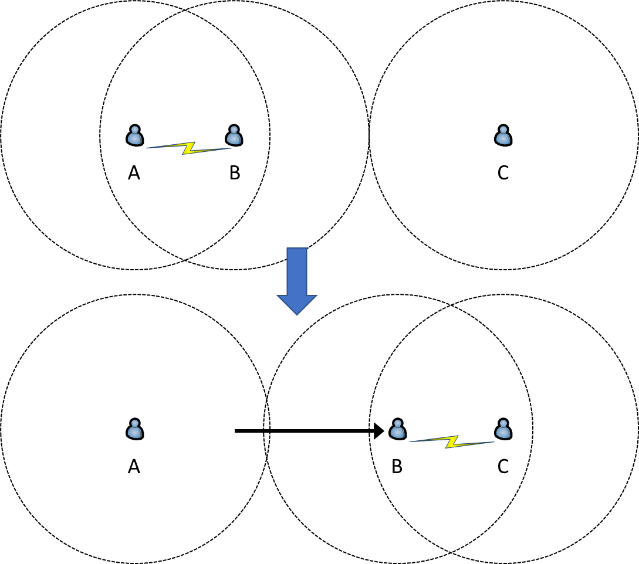
\includegraphics[width=4.0in]{figures/FIG_MANET.png}
  \caption{MANET} 
  \label{fig:MANET} %% label for entire figure 
\end{figure}

\section{ Delay Tolerant Network}

\noindent Regular networks, e.g. Internet, always have end-to-end paths. As shown in Figure 2.2, the node S and the node D are connected by A, B, and C. Their maximum round-trip time is not excessive, and their drop probability is also small. Comparing to the regular network, there is a class of challenged networks \cite {C1} which lacks end-to-end path and suffering from high latency and long queuing times. As shown in Figure 2.3, when the node B is not working, there is no connection between the node A and the node C, so that extensive latency is inevitable if the source S sends a message to the destination D.

\begin{figure} [H]
  \centering 
  \subfigure[Regular Network]{ 
    \label{fig:comparison_RN_DTN:a} %% label for first subfigure 
    
\includegraphics[width=4.0in]{figures/FIG_Regular_Network.png}} 
  \hspace{1in} 
  \subfigure[DTN]{ 
    \label{fig:comparison_RN_DTN:b} %% label for second subfigure 
    
\includegraphics[width=4.0in]{figures/FIG_DTN.png}}
  \caption{The comparison between regular networks and DTNs} 
  \label{fig:comparison_RN_DTN} %% label for entire figure 
\end{figure}

\noindent Since the challenged networks have significant differences with the regular networks, researchers introduce a new architecture Delay Tolerant Network (DTN) to deal with the unique features in the challenged works. Terrestrial Mobile Networks, Exotic Media Networks, Military Ad-Hoc Networks and Sensor/Actuator Networks are typical DTNs.


\subsection{ Spray and Wait}

\noindent The Spray and Wait is a known protocol for DTNs. Although it is not as efficient as protocols on internet, it works in DTNs. A message is initialized with several copies, a part of which are given to others when users encounter each other. Users keep forwarding copies until they each have only one copy of the message. When a user carrying at least one copy of the message encounters the destination, he gives all his copies to the destination to finish the delivery. The Binary Spray and Wait (BSW) is an optimized version of the Spray and Wait, which is also used in our protocols. The user who creates the message also makes several copies of that message. He gives half of the copies the user whom he encounters so that both he and the other user have a half of the copies. The users who get copies of the message continue to give a half of copies holding by them to others until they have only one copy. The remained one copy is given to the destination only.

\subsection{ Other Protocols}


\subsubsection{ Direct Contact Scheme}

\noindent The simplest strategy for DTN is that the source holds the message until he meets the destination, which is called the direct contact scheme. So, a direct path between the source and the destination is necessary for a success delivery. It is possible that the source never comes in contact with the destination so that message is not delivered. 


\subsubsection{ Replica Based Protocols}

\noindent The replica based protocols work by making several replicas of the message so that users can retransmit them upon connection establishment. The former BSW is also a kind of replica based protocols. Comparing to the direct contact scheme, the replica based protocols make it more possible for messages to be delivered. But they require more resources than the direct contact scheme because they need more memory to store the replicas. Therefore, making a reasonable decision for the message replication and dropping is the key to these kinds of protocols.


\subsubsection{  Knowledge-Based Protocols}

\noindent Different from the former replica protocols which require no knowledge about the topology of the network, the users in knowledge-based protocols try to evaluate their own view of the topology of the network so that they can make better forwarding decisions. However, the topology changes so frequently that it is hard for users to have an accurate topology.


\subsubsection{ Coding Based Protocols}

\noindent Authors in \cite {C12} and \cite {C13} make the approach by introducing coding techniques into routing protocols. Instead of making a few replicas, coding based protocols encrypts data to make a large number of message blocks. If the destination receives a part of the blocks, he can decrypt the message.

\section{ Location-Based Services}

\noindent The Location-Based Services (LBS) use users' location information to provide services, which is shown in Figure 2.4. Your smartphone can detect your coordinate and send it to LBS application server which is responsible to provide service based on the coordinate. The point of interest and the location advertisement are familiar instances of LBS. The LBS providers collect users' location information to provide services, which makes LBS providers a significant target of attackers. When attackers access the databases of the LBS providers, they can learn all sensitive information in the servers. So, the LBS providers should be viewed as semi-trusted, which might expose information in front of vicious attackers.

Users face risks of information breach when they access a semi-trusted LBS provider because anyone who has access to data in LBSs is able to steal and misuse LBS users' location-privacy. Considering that LBSs rely on location-aware computing, it is unavoidable to leak users' location from LBSs. Therefore, balancing ?these two competing aims of location privacy and location awareness? \cite {C20} is always a challenge.

\begin{figure} [H]
  \centering 
  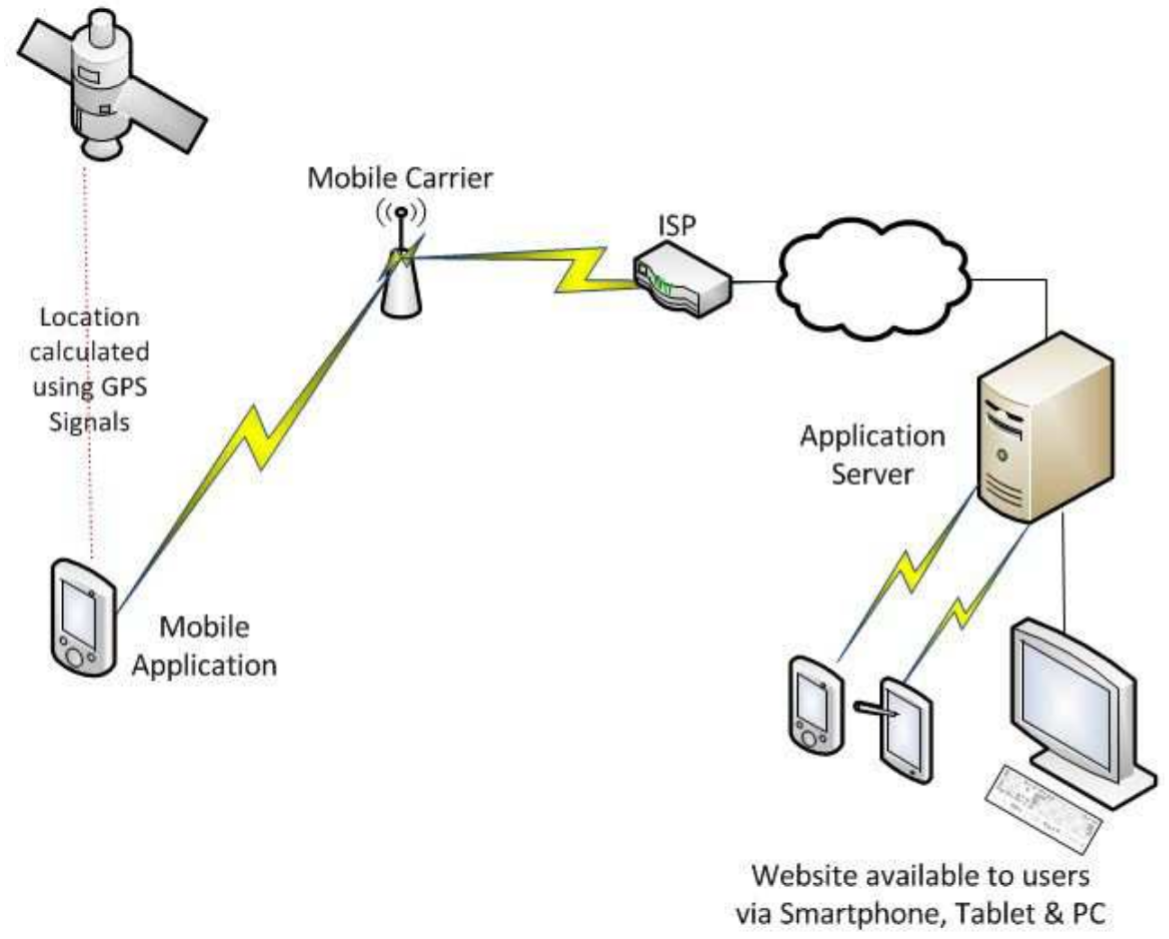
\includegraphics[width=4.0in]{figures/FIG_LBS_11.png}
  \caption{LBS \cite {C11}} 
  \label{fig:LBS} %% label for entire figure 
\end{figure}

\section{ Social Network}

\noindent Social networks which contains social interactions and personal relationships are used in location-privacy protection so that users can determine who is trustful. In \cite {C30}, the relationship of a pair of people (e.g., a user $i$ and a user $j$) is described as a pair of directed relationship strengths. The directed relationship strength from the user $i$ to the user $j$ can be denoted by ${RS}^{ij}$. We should notice that ${RS}^{ij}$ might be unequal to ${RS}^{ji}$, because the user $i$ might like the user $j$ so much while the user $j$ just views the user $i$ as an acquaintance. Based on the relationship strength, researcher can estimate the relational tie between two people and predict whether they are friends or strangers. 

The relationship strength is compared with a threshold, if the relationship strength is higher than the threshold the two people are friends, or they are strangers. In the protocols we mentioned in the thesis, researchers always assume that friends are trustful. That is reasonable because you might feel more secure when your friends forward your message instead of a stranger. 


\section{ Location-privacy protocols}

\noindent The basic idea of most location-privacy protocols is hiding the original requester behind a set of users so that attackers can hardly infer the identity of the original requester. In other words, when a user sends a query, his identity cannot be inferred based on the information in the query easily. For example, the original requester can use a pseudonym instead of his own name or use an obfuscated location to send his queries, so that attackers cannot tell the different between the queries and a set of other users' queries. 

The location-privacy protocols are considered as centralized and distributed ones based on whether they require any infrastructure. 


\subsection{ Centralized Protocols}

\noindent Centralized Protocols always need some infrastructure to serve for the obfuscation process. The infrastructure could be any equipment which act as anonymization servers. When users want to send a query to the LBS server, he sends the query to the anonymization server. The anonymization server changes the identity and the location in the query, which is called anonymization or obfuscation. Then the anonymization server forwards the modified query to the LBS server, so that the attacker who attacks the LBS server can hardly learn the identity of the original requester. The LBS server can send the reply message to the anonymization server which is responsible and able to forward the reply message back to the original requester. In this way, the original requester gets the information he needs, while avoiding from being located by attackers.

The advantage of the centralized protocols is that the anonymization server has more resources and information than users in the network, which enable the server to achieve better anonymization performance and provide sufficient protection for users. For example, if the anonymization server knows locations of all users in the network, it can modify the location and identity in the queries to the most suitable, with which the LBS server can provide acceptable results while the original requester is not exposed.

There are three major defects of this kind of protocol. 1. It is hard to deploy infrastructure in some area; 2. Since the anonymization server knows users' location, it is also a risk for users.


\subsubsection{ Single Server}

\noindent Authors in \cite {C15} uses a central anonymity server through which the mobile users can send queries to external services. To make the communication between users and the central anonymity server trustful, users set up an encrypted connection with the anonymity server at the beginning. Users sends their encrypted queries to the anonymity server, so that the anonymity server is the only one who can learn the information in the query. The anonymity server decrypts the queries and uses a cloaking algorithm to perturb the position information in the queries. Then the anonymity server sends the modified queries to external services (e.g. LBS). This is a typical centralized protocol, which can reduce the re-identification risk for users. Its defect is that a continuous connection to the server is necessary for each user, which is hard to achieve in a sparse DTN. We cannot image that a MANET user can have a stable connection with a central anonymity server, neither.

In \cite {C23}, researchers employ a matchmaker which is used to match users and advertisements, then users can achieve anonymization of their identities and locations from the matchmaker. The system architecture in \cite {C23} is similar to the former \cite {C}, while authors in \cite {C23} just focus on the advertisement service instead of the ?external services? in \cite {C23}. The role of matchmaker is matching users and advertisements. Although the functions of the matchmaker in \cite {C23} and the central anonymity server in \cite {C15} are different, the intermediate trusted three-party servers (i.e., the matchmaker and the central anonymity server) separate users and the application server (e.g., an advertisement server, LBS server and so on). The architecture in \cite {C23} does not require an encryption process so that attackers can learn the information in the queries. Although a plenty of queries arrive the matchmaker in a short time from different users also help the matchmaker mix the queries so that attackers can hardly trace the query, the burden of the users who are near the matchmaker is heavy.

In the work in \cite {C24}, researchers use ?a trusted, third-party location anonymization engine (LAE) that acts as a middle layer between mobile users and LBS providers? \cite {C24}, so that exact locations and requests from clients are replaced by a location anonymization engine before they arrive at LBS providers. Therefore, we learn that the structure of this kind of algorithms is almost like Figure 2.5. A trusted server is placed between users and the application server, which hides users' information and offers sufficient information for the application servers to provide acceptable services. 

\begin{figure} [H]
  \centering 
  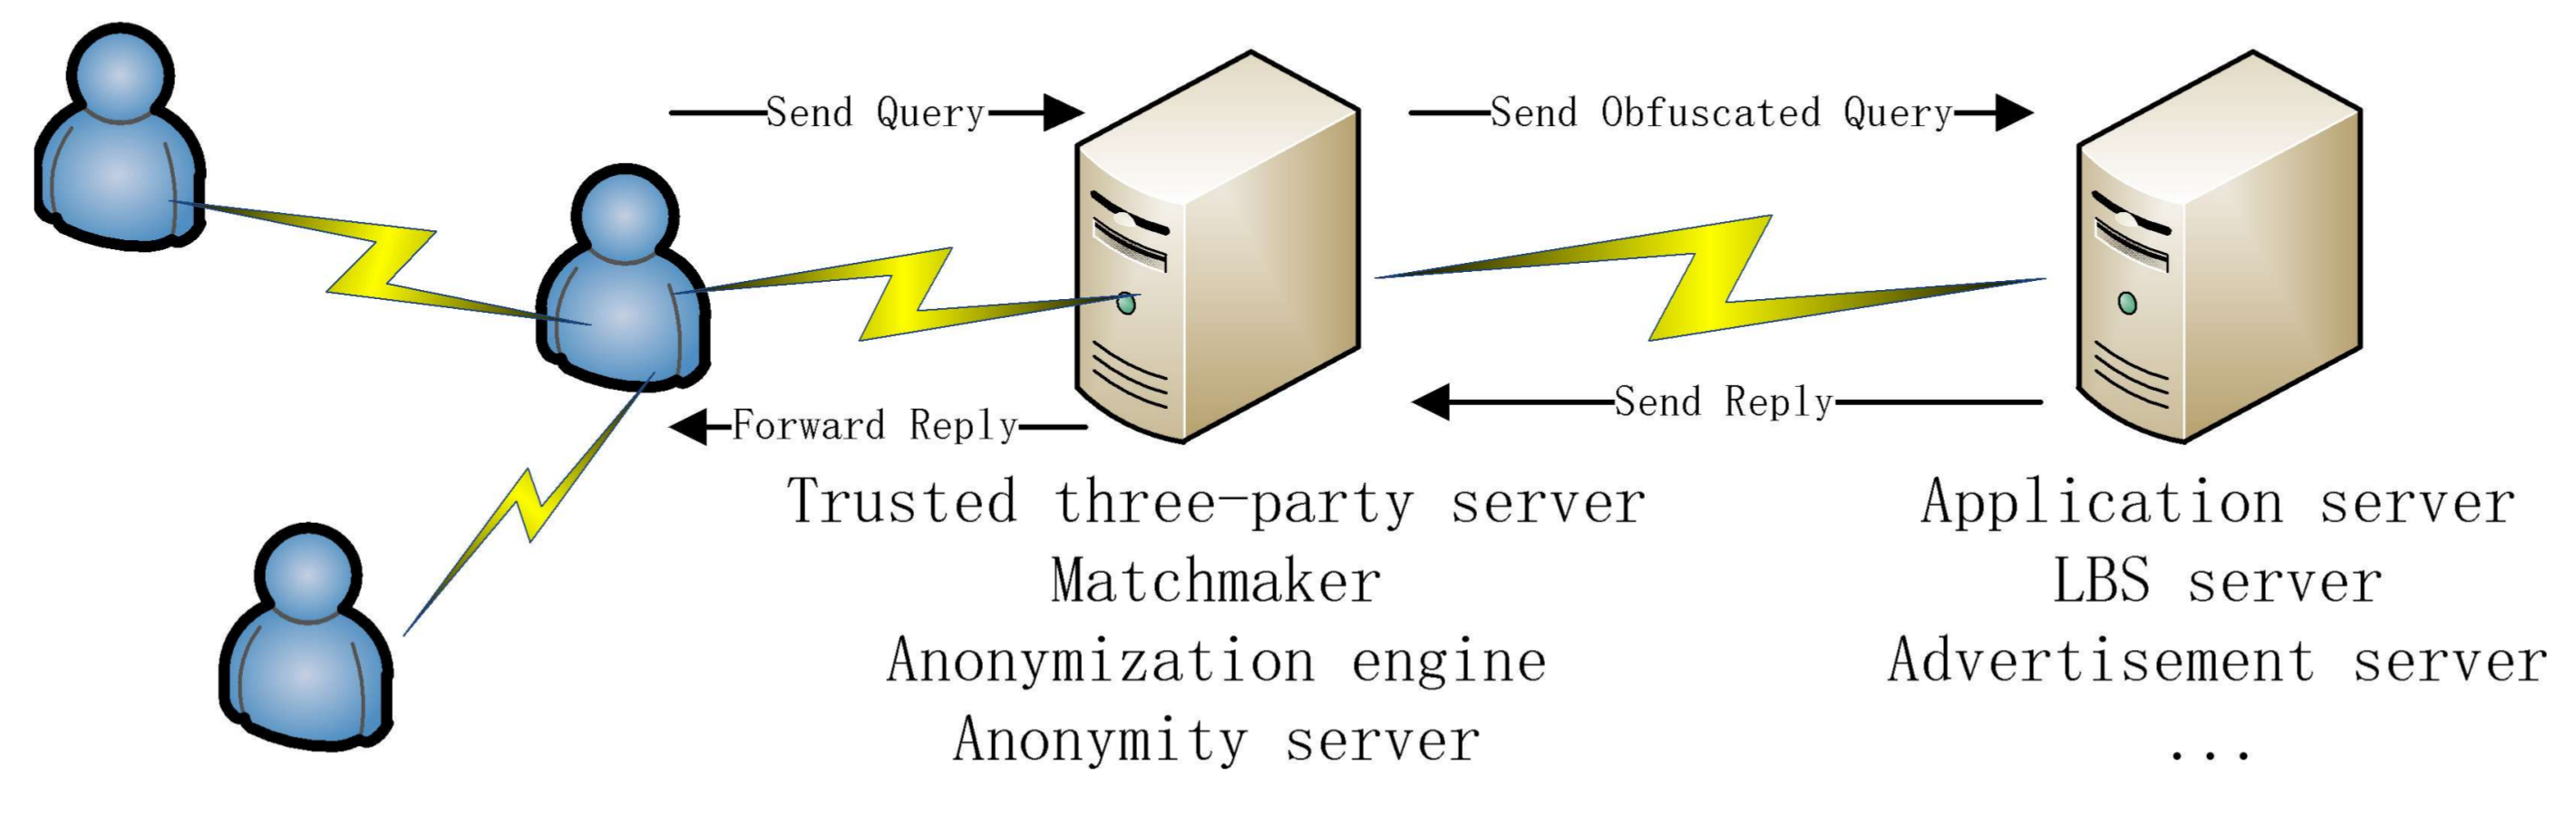
\includegraphics[width=4.0in]{figures/Fig_Single_Ano_Ser.png}
  \caption{Single Anonymization Server} 
  \label{fig:SingleAnoymizationServer} %% label for entire figure 
\end{figure}

\subsubsection{ Multiple Servers}

\noindent The above protocols always use a single anonymization server, while there are also other protocols which need more infrastructures. 

Authors in \cite {C25} propose a protocol, called Social-based PRivacy-preserving packet forwardING (SPRING), for vehicular delay tolerant network. In their work, they employ Roadside Units (RSUs), which are a type of equipment deployed along the roadside, to assist the packet forwarding and achieve conditional privacy preservation. These RSUs are located at high social intersections, so that vehicles which pass by the RSUs send their messages to the RSUs. The RSUs have sufficient resource so that they can hold the messages for a long time, which decrease the probability that the messages are dropped. The messages are forwarded to proper next-hop vehicles when the vehicles pass by the RSUs. Since messages are hold by the RSUs for a period, attackers can hardly trace messages. Besides, a large number of vehicles send many packets to these RSUs, which enables the RSUs to serve as mix servers. The advantage of SPRING is that it improves the delivery success ratio and privacy-protection performance. However, deploying the RSUs is not always feasible.

Another example is the work in \cite {C26}. Researchers use sensor nodes which are scattered throughout the network to provide anonymized locations for users, as shown in Figure 2.6. The whole system area is partitioned into a set of aggregate locations by the sensor nodes, where there are at least $k$ persons. To provide better location-based services, they minimize the areas of aggregate locations. When a user sends a query to the LBS, he uses the location of the sensor nodes which he belongs to, so that attackers cannot tell the difference between the requester and the other $k-1$ users in that aggregate location. This is a typical k anonymity algorithm, while its disadvantage is that it is difficult to deploy the sensor nodes in real-world. Besides, the mix servers and sensor nodes might be more prominent targets than LBS providers.

\begin{figure} [H]
  \centering 
  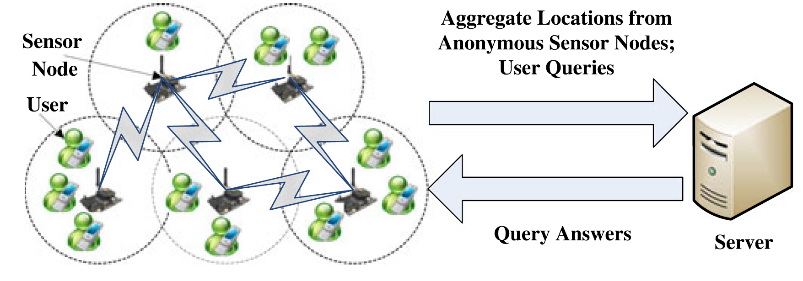
\includegraphics[width=4.0in]{figures/FIG_REAL_26.png}
  \caption{REAL \cite{C25}} 
  \label{fig:REAL} %% label for entire figure 
\end{figure}

\subsection{ Distributed Protocols}

\noindent Although centralized protocols also have good performance in their delivery success ratio and privacy-protection in their own field, the MANET is a network without infrastructure. In general, it is not allowed that deploy any infrastructure for MANET. Distributed protocols are organized by users independently so that they are more proper for applications in MANET. A problem for a distributed protocol it that whether a user can trust another one. Authors in \cite {C16}, \cite {C17} and \cite {C18} introduce the social tie to determine whether a user is trustful.

In the distributed social based location privacy protocol (SLPD) \cite {C16}, authors import 2 concepts: the obfuscation phase and the free phase. A query from an original requester is initialed as the obfuscation phase, then it must be transmitted between friends for $k$ times. For example, the original requester sends the query to one of his friend in one hop, then the friend forwards the query to another friend. We call these friends the agents. That process repeats for exact $k$ times. When the $k^{th}$ friend get the query, he switches the query to the free phase and replaces the sender identity with his own identity, then sends the query to the destination (e.g., LBS) with any DTN protocol. The LBS sends the reply to the friends and they are responsible to forward the message to the original requester. 

In this way, attackers can only learn the identity of the last friend instead of the original requester. Since each user who knows the identity of the original requester is the original requester's friend who are assumed trustful, there are no attackers among these agents. Therefore, attackers can hardly learn the identity of the original requester.

The disadvantage of the protocol is that it is hard to encounter a friend in the network, which decreases the success ratio of delivering queries. The how to improve the success ratio is a key of these protocols.

In Hybrid and Social-aware Location-Privacy in Opportunistic mobile social networks (HSLPO) \cite {C17}, authors try to improve the delivery performance by using a stochastic model which uses a Markov model for location predication. The major process is similar with SLPD, but an agent can forward the query a user who is not a friend of the original requester if the user has more chance to deliver the query and a trust value larger than a threshold. In other words, an agent continuously searching his surrounding to find the original requester's friends. If the agent cannot find the original requester's friend but his own friend, he checks whether his friend has more chance to deliver the query than him using the Markov model. If his friend is more proper for forwarding, he sends the query to his friend. The performance of HSLPO depends on the Markov model, that is, whether it can predict users' movement accurately. In our real-world, people's movement model is more complicated than that in experiment.

Another protocol, called Location Privacy-Aware Forwarding (LPAF) \cite {C18}, also attempt to improve the performance of the SLPD. The LPAF and the SLPD are similar, while the LPAF just add more friends to the protocol. When an agent cannot find a close friend (i.e., their trust value is high), he will try to find other general friends (i.e., their trust values is lower than the close friends). That might be a safety tradeoff, because some ineligible users in SLPD are chosen as friends based on the additional standards imported by LPAF.

In fact, both the HSLPO and LPAF cannot solve the problem in finding friends. Although we use the friends of friends or set the threshold for friends lower, there are only a few users can be chosen as agents. In LPAF, the identity of the requester is even exposed in front of someone who are not very trustful. 





















%%%%%%%%%%%%%%%%%%%%%%%%%%%
\chapter {Multi-Hop Location-Privacy Protection}
\label{C_MHLPP}
%%%%%%%%%%%%%%%%%%%%%%%%%%%

\section{ System Model}

\noindent Our network architecture consists of two main entities: Users and LBS Providers (LBSPs). Due to the introduction of the social network, the users' social information can be used in obfuscation forwarding process. Based on available information in the social network, the relationship between two users can be considered as friends or strangers. The user who makes a query to an LBSP will be called the original requester while the others are called intermediate users. LBSPs are located in fixed locations and their coordinates are known by all users when users join the network. Attackers are assumed to be able to access LBSPs, and attempt to locate original requesters. We assume that the LBSPs are semi-trusted and the strangers are un-trusted. We also assume that both entities have sufficient resources, like computational capability, storage and battery power.

Since two friends could be a pair of multi-hop neighbors, users can leverage Optimized Link State Routing Protocol \cite{C29} to seek friends continuously after entering the network, so that they can recognize each other and make contact in time. When a user carries an obfuscation phase query, he might send the query to a multi-hop friend through several strangers. In this case, a secure communication is necessary for between them, so that they must send the query encrypted to prevent strangers from learning anything about the query. Each user obtains a pair of asymmetric keys (public and secret key) before he joins the network from a certificate authority using well-regarded techniques, like in \cite{C28}. Whenever a user detects a new friend, he sends a request to the friend asking for his public key. In this way, a user can get his friends' public key when they encounter each other. Even though several strangers can be active in the obfuscation phase, the queries can still be securely sent to the user's friend.

The relationship strength is often ``a hidden effect of nodal profile similarities'' \cite{C30}. Let ${SV}_{i,j}$ denote a value of relationship strength which user $i$ determines whether user $j$ is an acceptable friend based on the relationship strength. For every pair of users ($i$ and $j$), we assume that there is an ${SV}_{i,j}$. If ${SV}_{i,j}$ is bigger than a specific friend threshold $T_{min}$, set by the original requester, user $j$ is considered as a friend of user $i$; otherwise, it will be treated as a stranger. The notations used in this chapter and their meanings are shown in Table \ref{table:MhlppSymbols}. 


\begin{table}
\caption{MHLPP Symbols}
\label{table:MhlppSymbols}
\centering
\begin{tabular}{|c|l|} \hline 
Parameter & Meanings \\ \hline 
\textit{N${}_{0}$} & the original requester \\ \hline 
\textit{N${}_{i}$} & if $i>0$, it denotes the friend chosen by ${N}_{i-1}$. \newline If $i=0$, it is ${N}_{0}$. \\ \hline 
\textit{N${}_{f}$} & the last friend who handles the obfuscation query \\ \hline 
\textit{N${}_{d}$} & the destination or the LBSP \\ \hline 
\textit{K${}_{i}$} & the public key of $N_i$ \\ \hline 
\textit{S${}_{i}$} & the secret key of $N_i$  \\ \hline 
\textit{q} & a query of $N_0$ \\ \hline 
\textit{r${}_{q}$} & the requirement for the query $q$ \\ \hline 
\textit{msg} & a message contains $q$ and ${r}_{q}$ \\ \hline 
\textit{Emsg${}_{i}$} & the encrypted $msg$ using ${K}_{i}$ \\ \hline 
\textit{S${}_{id}$} & the original requester's identity \\ \hline 
\textit{D${}_{id}$} & the destination's identity \\ \hline 
\textit{L${}_{s}$} & the location of ${N}_{0}$ when it sends the query to ${N}_{1}$ \\ \hline 
\textit{R${}_{p}$} & the inner radius of the \textit{obfuscation area} \\ \hline 
\textit{R${}_{s}$} & the external radius of the \textit{obfuscation area}  \\ \hline 
\textit{T${}_{min}$} & the social value bound for friends \\ \hline 
\textit{C${}_{max}$} & the extra path limit in each obfuscation forward \\ \hline 
\textit{${SV}_{i,j}$} & the relationship strength between user $i$ and $j$ \\ \hline 
\end{tabular}
\end{table}


\section{ Details of MHLPP}

\noindent MHLPP aims to protect the original requester's ($N_0$'s) location-privacy using an obfuscation path. In other words, a query $q$ which needs to be obfuscated must go through a series of friends after it leaves $N_0$. The whole process includes two parts: the obfuscation phase and the free phase. In the former phase, $q$ is only transmitted among friends, until it is sent to an area called ``\textit{obfuscation area}''. At the end of that phase the last friend $N_f$ replaces all $N_0$'s information by its own and forwards $q$ with an arbitrary DTN forwarding protocol, like the one suggested in \cite{C31}. In this case, what attackers can learn from the database in LBSP is $N_f$'s information, so they can hardly infer the original requester's identity and location based on that information. The free phase starts when the query $q$ is forwarded by $N_f$ and ends when it reaches the LBSP. 

Because $N_f$ is the only identity the LBSP knows, the LBSP has no choice other than replying to the last friend $N_f$ when it receives the obfuscated query. The reply can be delivered with an arbitrary DTN routing protocol as the free phase query does. The friend $N_f$ should remember who is the real destination ($N_0$) of this reply, then he transmits it to $N_0$. In this way, $N_0$ is able to send a query $q$ to an LBSP while not exposing his own information.

The obfuscation phase of a query $q$ starts when the query leaves the original requester $N_0$. When a user is holding an obfuscation phase query, he starts sensing connected friends continuously, which enables it to communicate with one-hop or multi-hop neighbor friends. Even though users in the mobile network use OLSR protocol \cite{C29} to detect others automatically, they do not communicate with their friend unless they have a requirement to send an obfuscation query. Also, they do not ask their friends for public keys. Therefore, carrying an obfuscation phase query requires a user to execute MHLPP algorithm.

When $N_0$ finds the first available friend $N_1$, he asks $N_1$ for a public key $K_1$, which will enable him to encrypt his query using $K_1$. That prevent others, e.g. strangers, from learning information in the message $msg$ that that contains both $q$ and $r_q$. $r_q$ is $N_0$'s requirement for $q$, which is always sent with the query $q$ and remains constant until the end of the obfuscation phase (we discuss this in section \ref{SecReqPara}). Friends who get the query can infer $q$'s \textit{obfuscation area} based on parameters $R_p$, $R_s$ and $L_s$ in $r_q$, which is a ring with inner radius $R_p$, external radius $R_s$ and center $L_s$. Before $N_0$ sends the query $q$ to his friend, he initializes parameter $L_s$ to his current location and encrypts $msg$ using $K_1$ to get ${Emsg}_1$ which is what $N_0$ sends to ${N}_1$.

The destination of ${Emsg}_1$ is ${N}_1$, which is a plaintext in ${Emsg}_1$, so that other intermediate users (strangers) can help $N_0$ forward ${Emsg}_1$ to ${N}_1$. In this step, strangers transmit ${Emsg}_1$ using the OLSR protocol if ${N}_1$ is a multi-hop neighbor of $N_0$. Strangers learn nothing other than the identity of ${N}_1$, because both $q$ and $r_q$ are encrypted. They cannot help attackers locate $N_0$ because they do not know ${S}_{id}$ (the identity of $N_0$) and ${D}_{id}$ (the LBSP) included in $r_q$.

When ${N}_1$ receives ${Emsg}_1$, he decrypts it with its secret key ${S}_{1}$ to get $q$ and $r_q$. If $q$ is already in the \textit{obfuscation area} defined in ${r}_{q}$ (i.e., it is already in the ring), the query $q$ finishes its the obfuscation phase. Then ${N}_1$ replaces all information of $N_0$ with his own. For example, the ${S}_{id}$ is replaced with ${N}_1$. If a location is necessary for the LBS, ${N}_1$ uses his own current location and records this change in his memory before initiating the free phase. A free phase query can then be forwarded to the destination (i.e., LBSP). 

If $q$ is still in the obfuscation phase (not in the ring), ${N}_1$ performs similar actions just as $N_0$ expect modifying $r_q$. Another difference is that instead of finding friend randomly, ${N}_{1}$ would seek for a friend who is nearer in the \textit{obfuscation area}, and so will the following friend. 

The detailed algorithm is explained in Algorithm \ref{AlgObfMhlpp} where ${N}_{x}$ is a neighbor of ${N}_{i}$ who is carrying the query $q$. Procedure ``$DealWithQuery$'' is responsible for dealing with a query. For $N_0$, he generates the query $q$ and its requirement $r_q$. If ${N}_{i}$ receives ${Emsg}_{i}$, he decrypts it with his own secret key ${S}_{i}$. If $q$ finished its obfuscation phase at ${N}_{i}$, $q$ will be required to be forwarded in free phase immediately. Otherwise, $q$ needs to be processed in the obfuscation process. Both $q$ and $r_q$ are stored in ${N}_{i}$ until they are sent to the next friend. ${N}_{i}$ starts detecting friends continuously if and only if ${N}_{i}$ carries one or more obfuscation phase queries. 

\begin{algorithm} [tbp]
\caption{The Obfuscation Phase in MHLPP}\label{AlgObfMhlpp}
\begin{algorithmic}[1]
\Procedure{DealWithQuery}{}
\If {the current user is $N_0$} 
	\State $generate\left (q,r_q\right)$ by himself
\Else 
	\If {the current user is $N_i$, $i>0$} 
		\State $\left (q,r_q\right) \gets {Decrypt}_{S_i}\left({Emsg}_i\right)$
	\EndIf
\EndIf

\If {$q$ can switch to the free phase based on $r_q$} 
	\State $SwitchFree\left(q\right)$
\Else 
	\State $msg \gets \left (q,r_q\right)$
	\State Store $msg$
	\State Start sensing friends
\EndIf
\EndProcedure

\Procedure{WhenEncounterUser}{$N_x$}
\State $q \gets$ get query from $msg$, $r_q \gets$ get requirement from $msg$
\If{$q$ timeout}
	\State remove $msg$
	\Return
\EndIf
\If{$q$ is eligible to switch into the free phase}
	\State $SwitchFree\left(q\right)$
	\Return
\EndIf
\If{${SV}_{i,x}$ is bigger than ${T}_{min}$ in $r_q$}
	\If{it is the first hop of $q$}
		\State assign the current location to $L_s$ of $r_q$
	\EndIf
	\State ${Emsg}_x \gets {Encrypt}_{S_x}\left(q,r_q\right)$
	\State forward ${Emsg}_x$ to $N_x$
	\State remove $msg$ from memory
	\State stop sensing friends
\EndIf
\EndProcedure

\Procedure{SwitchFree}{$q$}
\State ${q^*} \gets$ replace $q$'s requester-information ($N_0$) by $N_i$
\State record $\left(q,q^*\right)$
\State forward $q^*$ with DTN protocols
\EndProcedure
\end{algorithmic}
\end{algorithm}

When ${N}_{i}$ detects a new neighbor ${N}_{x}$ (one-hop or multi-hop neighbor), he follows steps in ``\textit{WhenEncounterUser}''. For an expired query, ${N}_{i}$ simply drops it. If the query $q$ is already inside its \textit{obfuscation area}, ${N}_{i}$ switches it to the free phase. If $q$ stays in the obfuscation phase and ${N}_{x}$ is an available friend, ${N}_{i}$ encrypts both $q$ and $r_q$ using ${N}_{x}$'s public key ${K}_{x}$ to get an encrypted message ${Emsg}_{x}$. Then ${N}_{i}$ forwards ${Emsg}_{x}$ to ${N}_{x}$ and stops sensing friends after ${Emsg}_{x}$ departs from it.

When we mention that ${N}_{i}$ switches a query $q$ to the free phase, ${N}_{i}$ actually replaces $N_0$'s information with its own one in $q$ to get ${q}^{*}$ and records this replacement in its storage, then ${N}_{i}$ uses the Spray and Wait protocol \cite{C31} to forward ${q}^{*}$ in plaintext. That allows ${N}_{i}$ to hide $N_0$'s identity and forward a reply from LBSP to $N_0$.


\section{ Requirement parameters} \label{SecReqPara}

\noindent In the obfuscation phase, ${r}_{q}$ is always in $msg$ so that friends who get $msg$ can make decisions (e.g. selections of friends) based on it.

All parameters (i.e., ${S}_{id}$, ${D}_{id}$, ${R}_{p}$, ${R}_{s}$, ${L}_{s}$ ,${T}_{min}$ and ${C}_{max}$) in ${r}_{q}$ are given by ${N}_{0}$ before ${Emsg}_{1}$ leaves ${N}_{0}$. Parameters ${S}_{id}$ and ${D}_{id}$ record the identities of ${N}_{0}$ and the destination (LBSP) ${N}_{d}$, based on which last friend ${N}_{f}$ is able to send the query freely to ${D}_{id}$ (${N}_{d}$) and forward the reply to ${S}_{id}$ (${N}_{0}$).

The obfuscation area is a ring with an inner radius ${R}_{p}$ and an external radius ${R}_{s}$. As shown in Figure \ref{fig:SelectionOfNxtFriend:a}, the obfuscation area is actually the grey area ``$a$''. \textit{obfuscation area} must guarantee both the original requester's location-privacy and location awareness. In other words, the value of ${R}_{p}$ should be big enough, so that there are sufficient users in the inner circle (with a radius ${R}_{p}$). At the same time, ${R}_{s}$ should be small enough so that the LBSP can provide a service, acceptable to ${N}_{0}$. 


\begin{figure} [H]
  \centering 
  \subfigure[The Ring]{ 
    \label{fig:SelectionOfNxtFriend:a} %% label for first subfigure 
    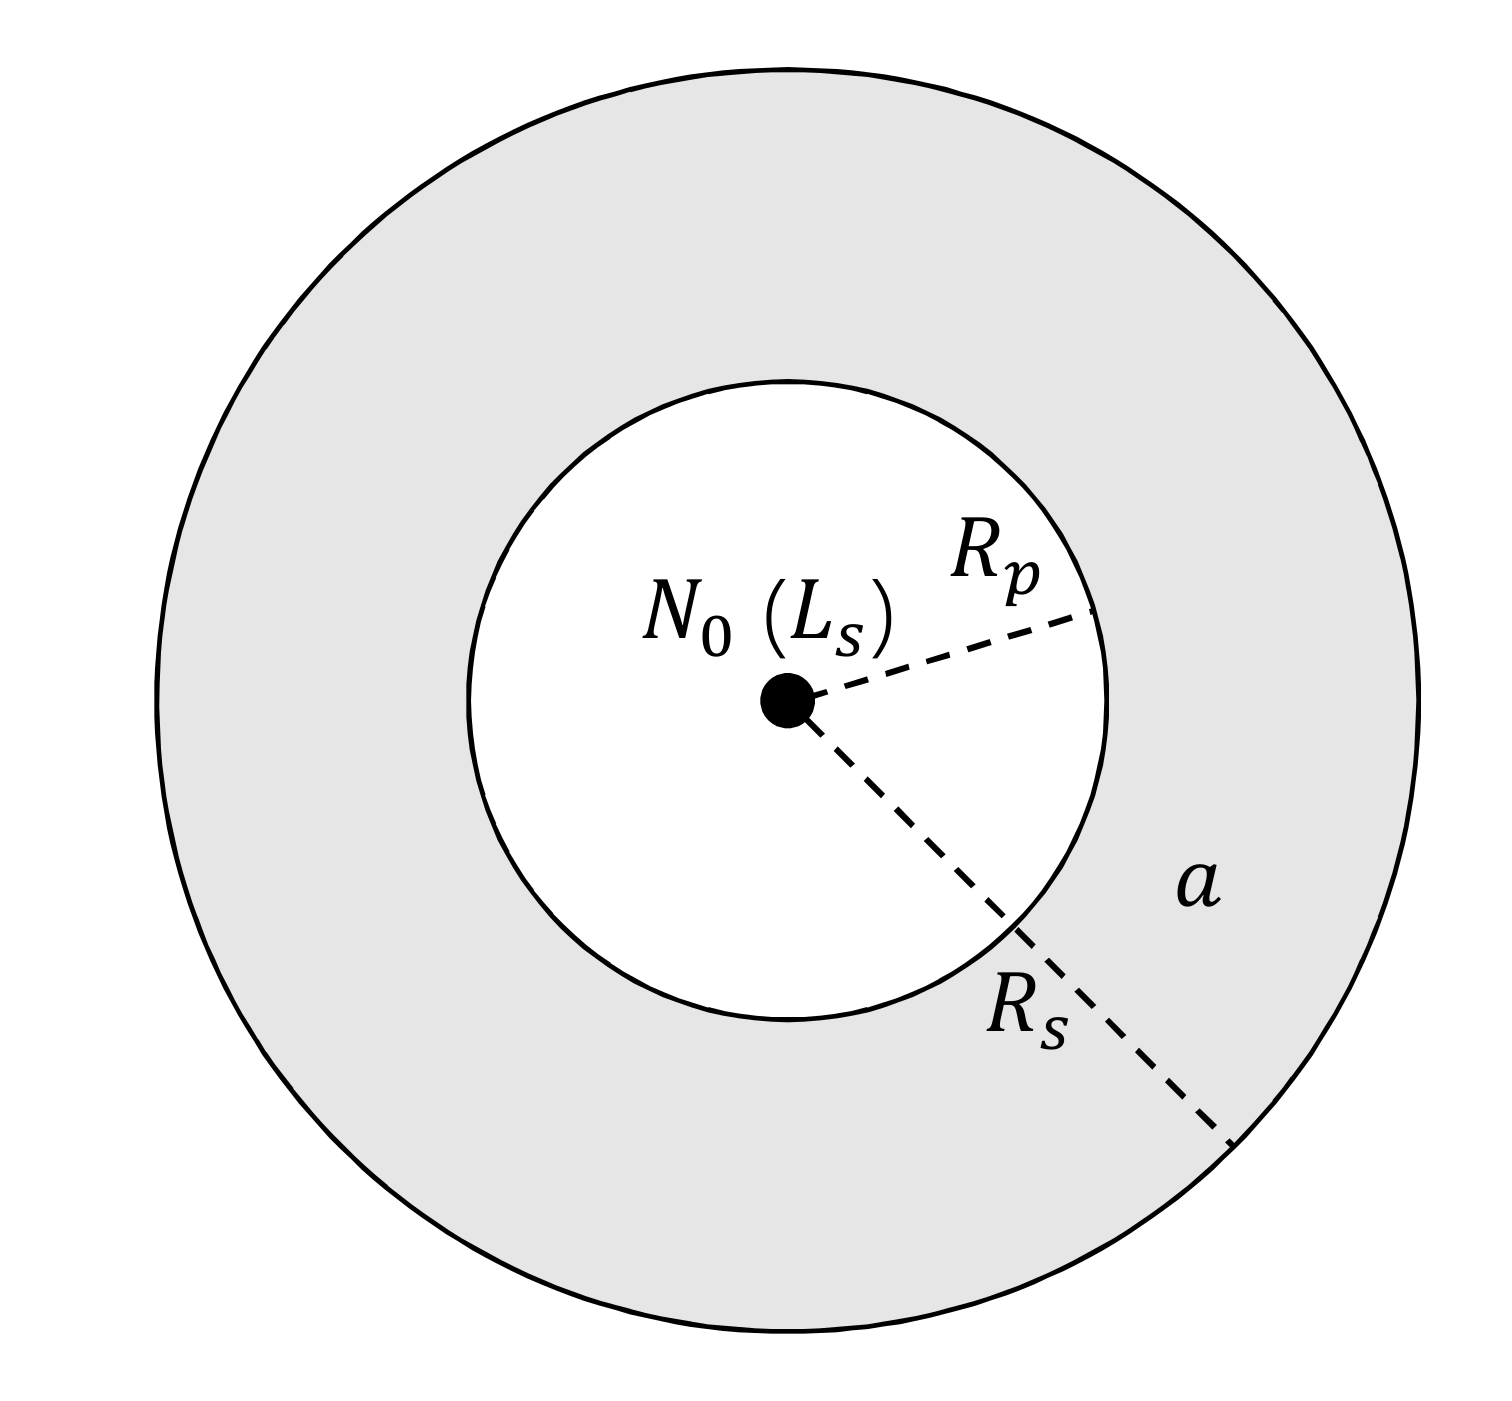
\includegraphics[width=2.5in]{figures/findnf_a.png}} 
  \subfigure[The Agent And The Destination]{ 
    \label{fig:SelectionOfNxtFriend:b} %% label for second subfigure 
    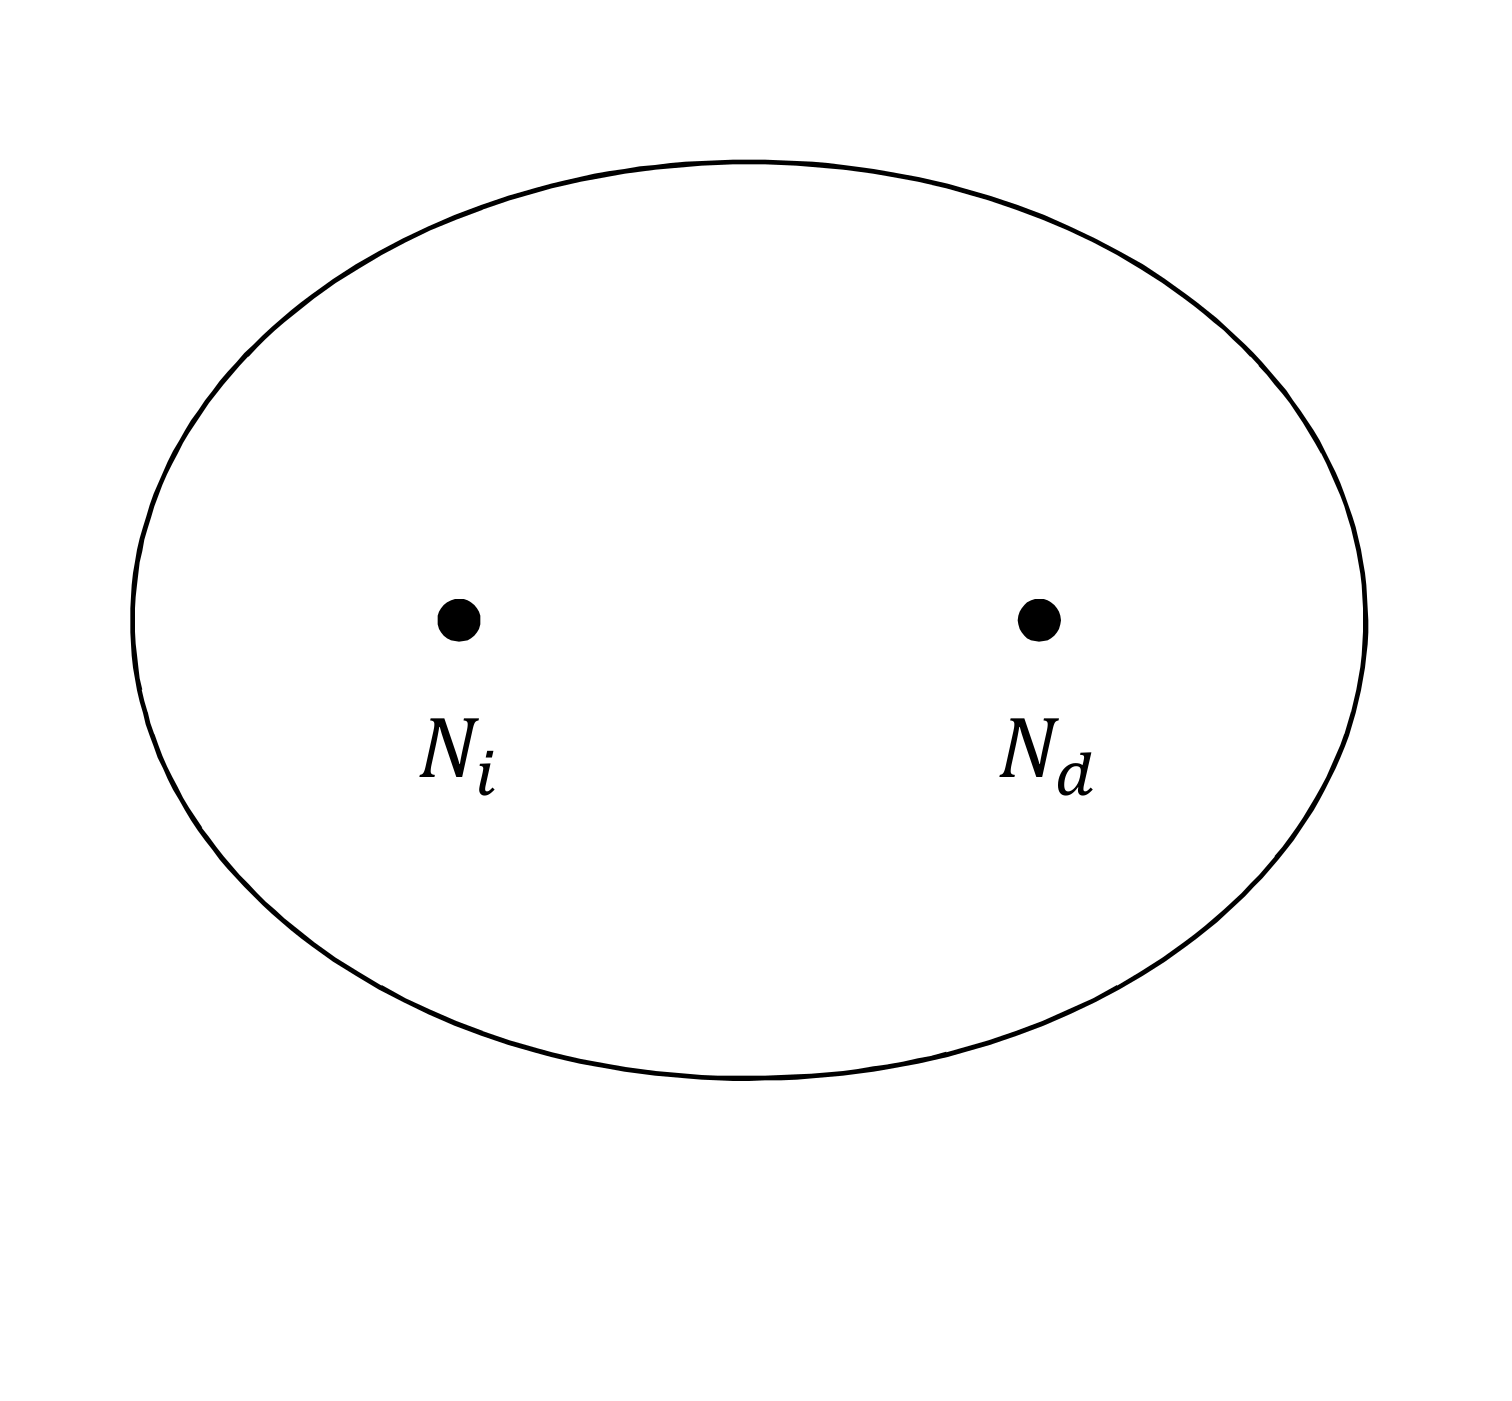
\includegraphics[width=2.5in]{figures/findnf_b.png}}
  \caption{The Selection Of The Next Friend} 
  \label{fig:SelectionOfNxtFriend} %% label for entire figure 
\end{figure}

A user ${N}_{x}$ can be chosen by ${N}_{i}$ as a friend for $q$ if and only if ${SV}_{i,x}$ is bigger than the threshold ${T}_{min}$. The original requester ${N}_{0}$ can set various values for his queries based on their importance. If ${T}_{min}$ is large, there would be fewer friends for any users in the network which reduces the query success rate to a certain extent, as a result. We assume that the original requester can balance the level of privacy and the success ratio. 

Most DTN routing protocols aim to deliver queries through the shortest path, while MHLPP pays more attention to security in its obfuscation phase. Consequently, the obfuscation process in MHLPP results in a longer path from the original requester ${N}_{0}$ to the destination ${N}_{d}$. To limit the length of the path, we introduce parameter ${C}_{max}$ which is the maximum extra path (e.g., the difference of the length and the distance between the ${N}_{i}$ and LBSP) we can tolerate. For any friend ${N}_{i}$ who gets a ${C}_{max}$ from ${r}_{q}$, if he selects ${N}_{x}$ as the next friend, the extra path should not be longer than ${C}_{max}$. Let's denote the optimal path from user $m$ to $n$ by ${Dis}\left (m,n\right )$, and the extra path from ${N}_{i}$ to ${N}_{d}$ through ${N}_{x}$ by ${C}_{i,x,d}$. Then ${C}_{i,x,d}$ can be defined as follow.

\begin{equation} \label{GrindEQ__1_} 
C_{i,x,d} =Dis(i,x)+Dis(x,d)-Dis(i,d) 
\end{equation} 

${C}_{i,x,d}$ must be a value smaller than ${C}_{max}$. If ${Dis}\left (m,n\right )$ is the straight-line distance between point $m$ and $n$, then next friend ${N}_{x}$ should be in an ellipse ${E}_{C}$ with focus points ${N}_{i}$ and ${N}_{d}$. Let's denote the coordinate of ${N}_{i}$ by $\left(-\frac{d}{2} ,0\right)$ and the coordinate of ${N}_{d}$ by $\left(\frac{d}{2} ,0\right)$. Then, the equation of the ellipse ${E}_{C}$ is

\begin{equation} \label{GrindEQ__2_} 
\frac{x^{2} }{\left(d+C_{\max } \right)^{2} } {\rm +}\frac{y^{2} }{2d\cdot C_{\max } +C_{\max }^{2} } {\rm =}\frac{1}{4}  
\end{equation}

As shown in Figure \ref{fig:SelectionOfNxtFriend:a}, ${L}_{s}$ is the center of the ring while ${R}_{p}$ and ${R}_{s}$ are the inner and external radii, respectively. The query $q$ switches to the free phase when it enters the ring area. 

As shown in Figure \ref{fig:SelectionOfNxtFriend:b}, ${N}_{i}$ who is carrying obfuscation queries should choose his next friend ${N}_{x}$ in the ellipse, which avoids the query $q$ going through an unacceptably long path.

In conclusion, a query $q$ starts at the center and moves inside the ring, until it reaches the \textit{obfuscation area}. The point ${N}_{i}$ in Figure \ref{fig:SelectionOfNxtFriend:b} should be inside the ring, and the point ${N}_{d}$ might be anywhere. As a result, a user ${N}_{i}$ who is carrying an obfuscation query detects a friend continuously who has a larger distance from ${L}_{s}$ and inside an ellipse. If there is a friend like that, ${N}_{i}$ sends the query to that friend ${N}_{x}$.

\section{ Privacy Analysis}

\noindent We assume that attackers can achieve all information in LBSPs know. Obviously, they can know the identity of the last friend $N_f$ who replaces ${N}_{0}$'s information with his own. It is possible for the attackers to locate $N_f$ with little cost. For example, if ${N}_{0}$ stops moving after sending the query $q$, it is reasonable for $N_f$ to believe that ${N}_{0}$ is in a ring centered at the location of itself with radii ${R}_{p}$ and ${R}_{s}$. In other words, the distance between ${N}_{f}$ and ${N}_{0}$ should be in a range between ${R}_{p}$ and ${R}_{s}$. If attackers find all users who satisfy this condition, the original requester might be among these users with high probability. Then, a success ratio $P_{r_pr_s}$ to locate ${N}_{0}$ can be measured by a conditional probability
\begin{equation} \label{GrindEQ__3_} 
P_{r_{p} r_{s} } =p_{r_{p} r_{s} } \cdot \frac{1}{m_{r_{p} r_{s} } }  
\end{equation} 
where $P_{r_pr_s}$ is the probability that ${N}_{0}$ is in the ring (i.e., the distance between ${N}_{0}$ and ${N}_{f}$ is larger than ${R}_{p}$ and smaller than ${R}_{s}$). Here, $m_{r_pr_s}$ is the number of users who are in the ring. Attackers locate ${N}_{0}$ successfully if and only if ${N}_{0}$ is in the ring, at the same time, attackers pick the correct one from all $m_{r_pr_s}$ users at that area.

In the worst case, attackers know exact values $R_s$ and $R_p$. Then, the Eqn. \eqref{GrindEQ__3_} becomes 
\begin{equation} \label{GrindEQ__4_} 
P_{R_{p} R_{s} } =p_{_{R_{p} R_{s} } } \cdot \frac{1}{m_{_{R_{p} R_{s} } } }  
\end{equation} 
where $P_{r_pr_s}$ is the probability that ${N}_{0}$ is on the ring (i.e., the distance between ${N}_{0}$ and ${N}_{f}$ is larger than ${R}_{p}$ and smaller than ${R}_{s}$). $m_{r_pr_s}$ is the number of users who are in the ring. Since parameters (e.g., ${R}_{p}$ and ${R}_{s}$) in ${r}_{q}$ are kept secret among trusted friends in our system model, attackers can hardly get the actual values of those parameters.

\section{ Complexity discussion}

\noindent In order to guarantee secure communications among friends, encryption is introduced in our protocol. In the obfuscation phase, the query is transmitted along friends, i.e., ${N}_{0}$, ${N}_{1}$, ${N}_{2}$, ..., ${N}_{f}$. When the query is sent from ${N}_{i}$ to ${N}_{i+1}$, a pair of encryption and decryption is needed, so the number of such pairs $T_{en}$ should be equal to $f$. 

$T_{en}$ grows with both ${T}_{min}$ (threshold used to decide friend relationship) and inner radius ${R}_{p}$. Essentially, it is the number of friends participating in transmitting a query $q$ in its obfuscation phase that influences $T_{en}$. Given a smaller ${T}_{min}$, a user carrying the obfuscation phase query has more chances to encounter more friends in a certain area. A larger ${R}_{p}$ also leads to a bigger area inside the ring, so that there are more friends in this area. We evaluate the number of encryptions and decryptions in our simulation. Figure \ref{fig:NumOfEncWithInnerR} shows the average number of encryptions ($T_{en}$) with different friend thresholds ${T}_{min}$ and inner radius ${R}_{p}$. We observe that $T_{en}$ increases steadily as we increase ${T}_{min}$ (i.e., 85\%, 90\%, and 95\%) and ${R}_{p}$ (i.e., the horizontal axis).

\begin{figure} [H]
  \centering 
  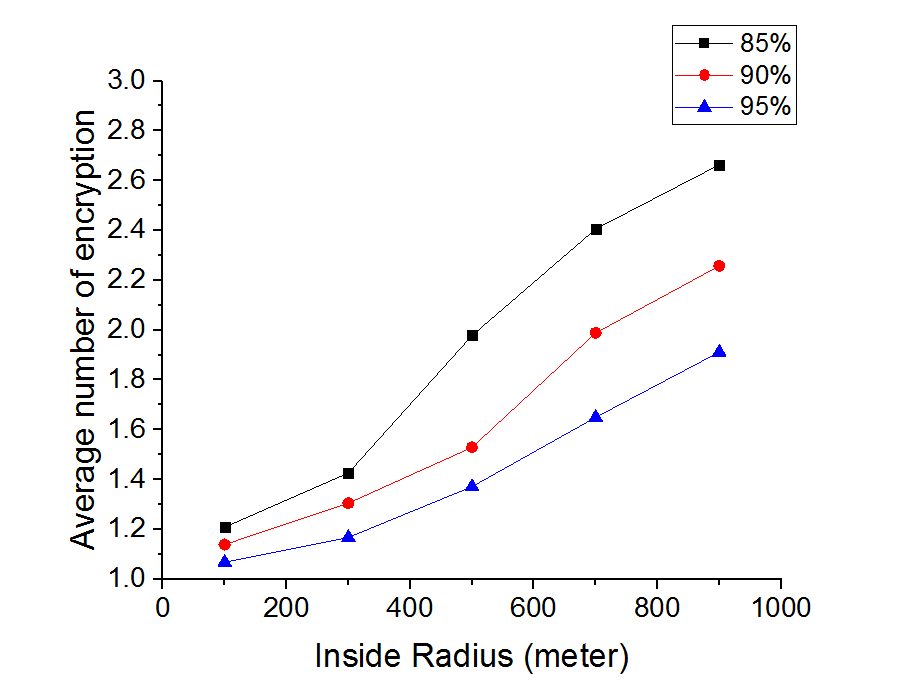
\includegraphics[width=4.0in]{figures/NumOfEncWithInnerR.png}
  \caption{The Number Of Encryption With Various Inner Radius} 
  \label{fig:NumOfEncWithInnerR} %% label for entire figure 
\end{figure}

It is evident that encryption and decryption process in MHLPP results in an extra cost in both energy and computational resources. However, the number of encryptions and decryptions is quite low (below 3) which reasonable based on the experiment.

\section{ Performance Analysis}

\noindent We use the map of Helsinki in our simulator to evaluate MHLPP. It is also compared against the known protocol, Hybrid and Social-aware Location-Privacy in Opportunistic mobile social networks (HSLPO). The simulation parameters are shown in Table \ref{table:MhlppExperimentParameters}. All pedestrians and cars are users in MHLPP. These users are moving on the map along streets continuously. There is an LBSP fixed at a random location on the map. For each user, we give him random social values between 0\% and 100\%, each corresponding to all other users. Each value has the same probability, so we can compute the expected number of friends of a user. For example, if we are given a privacy threshold (${T}_{min}$) of 85\%, then there might be 15\% (100\%-85\%) users who are friends of a certain user.

As shown in Table \ref{table:MhlppExperimentParameters}, there are 126 users in the map. For each of them, say user $i$, we give him 126 random $SV$ values, which denotes the relationship strength between him and other users, so that there are ${126}^2$ $SV$s in our simulation. The $SV$s are between 0 and 100. As a result, if the ${T}_{min}$ is equal to 85, the average number of friends of each user should be 18.9 (=$126\times (100-85)/100$).

\begin{table} [hbtp]
\caption{MHLPP Experiment Parameters}
\label{table:MhlppExperimentParameters}
\centering
\begin{tabular}{|l|l|} \hline 
Parameter & Value \\ \hline 
Simulation Time & 10 minutes \\ \hline 
Map Size (W x H) & 4500 m x 3400 m \\ \hline 
Total number of users & 126 \\ \hline 
Pedestrians/ Cars & 84/42 \\ \hline 
Communication Area Radius & 10m -- 90 m \\ \hline 
Pedestrian Speed & 1.8-5.4 Km/h \\ \hline 
Car Speed & 10-50 Km/h \\ \hline 
\end{tabular}
\end{table}

Users are placed at random locations at the beginning of each experiment. We choose another random point for each user, so that he can move back and forth along streets between that point and the point his starts at. The user speed depends on its type (pedestrians or cars) and set randomly. All queries have a 10-minute timeout. The queries which are expired before they reach the LBSP (the destination) are considered to be failed in our success ratio statistics.

Figures \ref{fig:QSR}-\ref{fig:LPE} compare performances between HSLPO and MHLPP for different values of $k$, communication radius and privacy threshold (${T}_{min}$ in MHLPP). The $k$ is the privacy-level requirement in HSLPO. Both HSLPO and MHLPP have different criteria in which a query can switch to the free phase. To make them comparable, we create a new parameter, called \textit{obfuscation distance}. If a query leaves ${N}_{0}$ at location ${L}_{a}$ and switches to the free phase at ${N}_{f}$ whose location is ${L}_{b}$, then the obfuscation distance is the straight-line distance between ${L}_{a}$ and ${L}_{b}$. We test the obfuscation distances of HSLPO with different parameters, and then we set the inner radius of MHLPP to those values. The query success ratio is the ratio of delivered queries to the total number of queries. The number of hops ($h$) is the number of intermediate users between ${N}_{0}$ and the destination (LBSP). We count the number of users surrounding the last friend in a specific range, which is $k$ times the communication radius. We calculate the entropy using the reciprocal of the number of surrounding users.

\subsection{ Query success ratio}

\noindent The query success ratio is the percentage of delivered queries among a number of attempts. Based on the timeout value in Table \ref{table:MhlppExperimentParameters}, a query is delivered successfully, if it arrives at the LBSP (the destination) before the timeout; otherwise it fails. We use the query success ratio to evaluate the delivery performance of MHLPP.

\begin{figure} [H]
  \centering 
  \subfigure[Query Success Ratio Versus Various $k$]{ 
    \label{fig:QSR:a} %% label for first subfigure 
    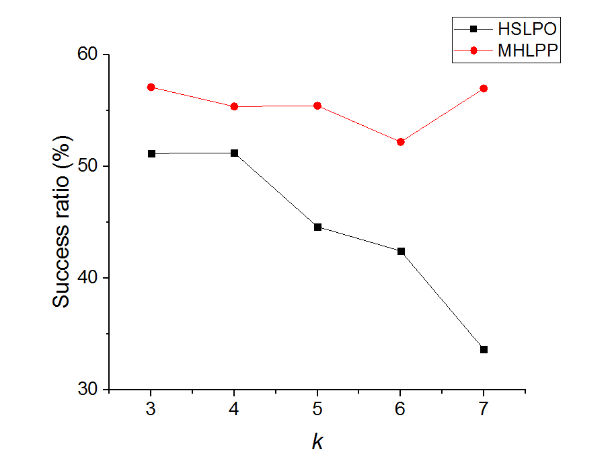
\includegraphics[width=3.0in]{figures/QSRa.png}} 
  \hspace{1in} 
  \subfigure[Query Success Ratio Versus Various Communication Radius]{ 
    \label{fig:QSR:b} %% label for second subfigure 
    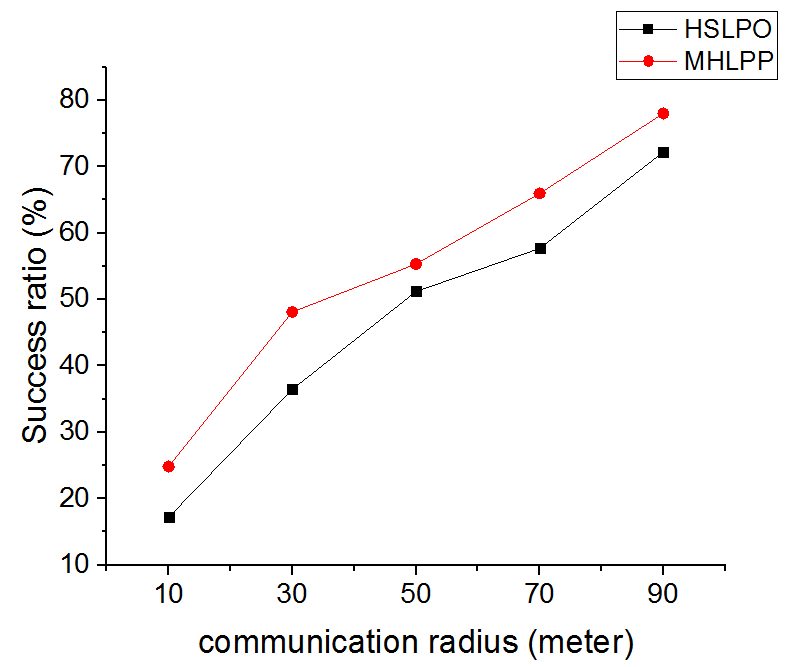
\includegraphics[width=3.0in]{figures/QSRb.png}}
  \hspace{1in} 
  \subfigure[Query Success Ratio Versus Various Privacy Thresholds]{ 
    \label{fig:QSR:c} %% label for second subfigure 
    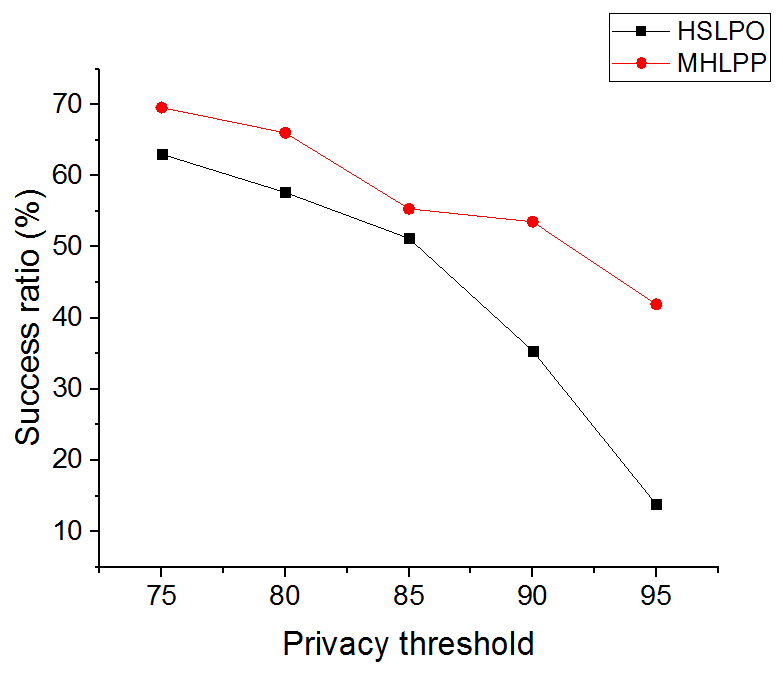
\includegraphics[width=3.0in]{figures/QSRc.png}}
  \caption{The Query Success Ratio Comparison Between HSLPO and MHLPP} 
  \label{fig:QSR} %% label for entire figure 
\end{figure}

As shown in Figure \ref{fig:QSR:a}, the success ratio in MHLPP is always higher than that in HSLPO. As the value of $k$ increases, HSLPO success ratio drops sharply while MHLPP remains stable. This is because the larger $k$ is, the harder it is for HSLPO to find enough friends in a limited time. The lack of friends has less impact on MHLPP. We observe that the success ratio of MHLPP rises when $k=7$. That is because it depends on the inner radius which is equal to the obfuscation distance of HSLPO. The obfuscation distance decreases when $k=7$, because most of the queries which complete their obfuscation phase have a short obfuscation distance. In Figure \ref{fig:QSR:b}, both HSLPO and MSLPP values increase and have the same trend when given a larger communication radius. The reason is that the communication radius effects the free phase more than the obfuscation phase for both. As shown in Figure \ref{fig:QSR:c}, higher privacy threshold leads to lower success ratio in two algorithms. Its impact on HSLPO is more intense than that on MHLPP, which is the most important characteristic of MHLPP. MHLPP has a better performance than HSLPO especially when there are fewer friends in the network. MHLPP can transmit messages with the help from strangers in its obfuscation phase while HSLPO cannot. 

\subsection{ Number of Hops}

\noindent We count the number of hops it takes for queries to be delivered successfully and calculate the average. Every user who takes part in the delivery process is considered in the hop count. We introduce this criterion to measure the routing path length of the algorithm. MHLPP is more sensitive to the probability that a user encounters a friend than HSLPO is. The reason is that MHLPP aims to reach a certain distance rather than taking certain number of hops. In other words, MHLPP continues sending queries to other friends until queries enter their \textit{obfuscation area}. In this process, MHLPP takes every chance to forward queries. If it is hard for MHLPP to find friends, it can also take the queries to obfuscation areas with fewer friends. Therefore, the probability that users encounter friends has less impact on the performance of MHLPP. The result is shown in Figure \ref{fig:NOH}.

\begin{figure} [H]
  \centering 
  \subfigure[Number Of Hops With Various $k$]{ 
    \label{fig:NOH:a} %% label for first subfigure 
    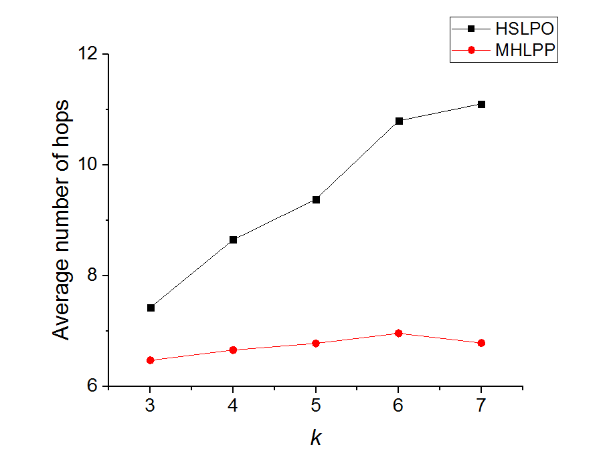
\includegraphics[width=3.0in]{figures/NOHa.png}} 
  \hspace{1in} 
  \subfigure[Number Of Hops With Various Communication Radii]{ 
    \label{fig:NOH:b} %% label for second subfigure 
    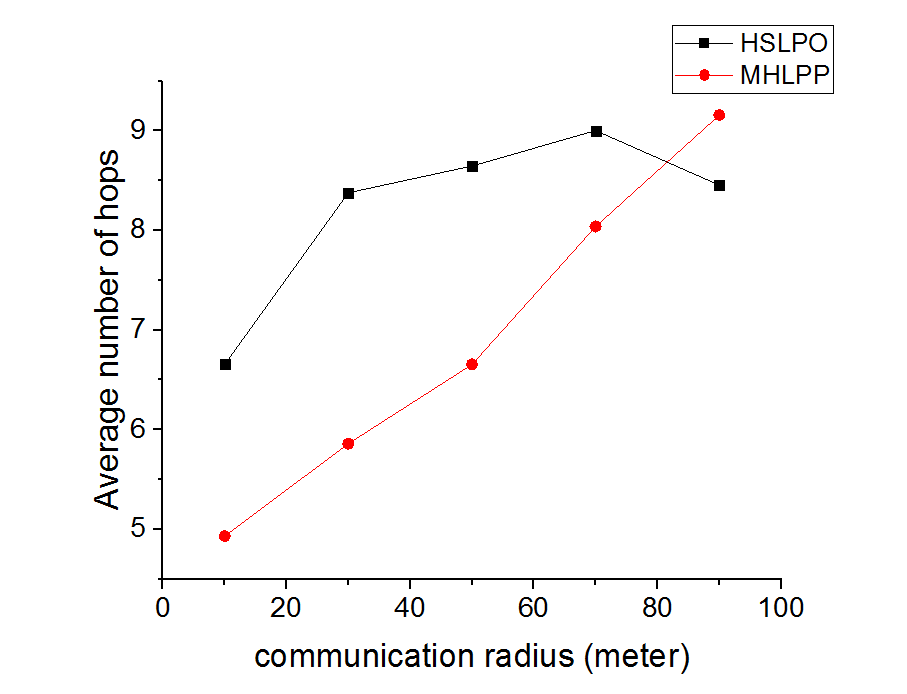
\includegraphics[width=3.0in]{figures/NOHb.png}}
  \hspace{1in} 
  \subfigure[Number Of Hops With Various Privacy Thresholds]{ 
    \label{fig:NOH:c} %% label for second subfigure 
    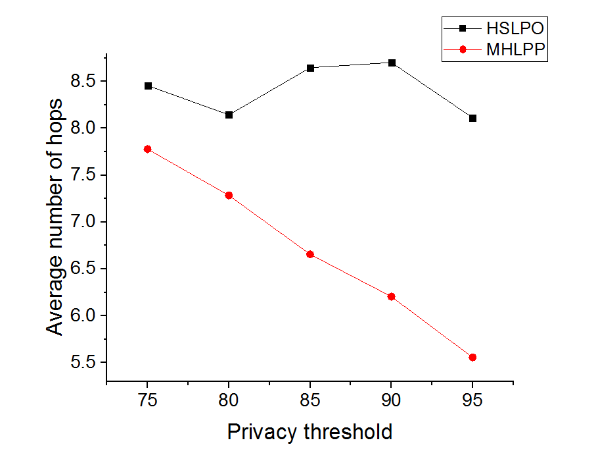
\includegraphics[width=3.0in]{figures/NOHc.png}}
  \caption{The Number Of Hops Comparison Between HSLPO And MHLPP} 
  \label{fig:NOH} %% label for entire figure 
\end{figure}

In Figure \ref{fig:NOH:a}, the number of hops in HSLPO is affected by parameter $k$ obviously. Especially, the first $k$ hops forwarders must be friends, which makes it hard for HSLPO to have queries to be forwarded successfully. Both protocols have similar number of hops in their free phases, but HSLPO has exactly $k$ hops in its obfuscation phase, while MHLPP can have fewer than $k$ hops. In figure \ref{fig:NOH:b}, the number of hops in MHLPP grows with the communication radius obviously, while it does not change a lot in HSLPO, because only successful delivery queries are counted in the statistics. Given a large communication radius, MHLPP has a much higher success ratio for delivered queries as it can connect more friends. In Figure \ref{fig:NOH:c}, the value of MHLPP drops for higher privacy thresholds. The reason is the same as Figure \ref{fig:NOH:b}. For HSLPO, no matter how hard it is to find a friend, it attempts to find exactly $k$ friends. However, if it is too hard to find a friend, MHLPP's friend can carry the query while moving and complete the obfuscation process. For higher privacy thresholds (i.e., resulting in fewer friends), MHLPP chooses to carry queries other than finding friends. That results in a drop in the number of hops.


\subsection{ Security}

\noindent Since the principles with that two protocols protect original requesters are different, we evaluate the probability that attackers locate the original requester if the distance between him and the last friend is smaller than a some value $r$, which is equal to $k$ times the communication radius. Since the last friend reveals himself to the LBSP, attackers might locate him accurately. We assume that attackers know the privacy parameter $k$. In the worst case, the distance between the original requester and the last friend is smaller than $r$ when attackers start to locate the original requester. That gives attackers a chance to locate the original requester. We count all users who are inside the radius $r$ of the last friend, and the original requester is one of them. For example, if there are $m$ users in the area, the probability should be $\frac{1}{m}$. Figure \ref{fig:LPE} compares the entropy $E$ of both HSLPO and MHLPP. We use the following formula for computing entropy:
\begin{equation} \label{GrindEQ__Entropy_} 
E=-\frac{1}{m}{log}_2\left(\frac{1}{m}\right)
\end{equation}

From Figure \ref{fig:LPE:a}, we observe that MHLPP has very small (about 0.04) increase in entropy compared to HSLPO. When the original requester is in the circle centered at the last friend, HSLPO is a little more secure than MHLPP but not by very much. That is because HSLPO always switches to the free phase when the last friend encounters the previous friend, so the previous friend must in the circle. MHLPP does not have this condition. Both graphs in Figure \ref{fig:LPE:a} and Figure \ref{fig:LPE:b} have the same trend. The curve of MHLPP is also a little higher than that of HSLPO, while two curves almost meet when the communication radius is small or large. Given a small radius, the entropy of both protocols are small. When the radius is large, we can ignore the effect of the previous friend mentioned about for Figure \ref{fig:LPE:a} as there are so many users in the circle. From Figure \ref{fig:LPE:c}, since the circle neither expands or shrinks, we observe that the two curves exhibit similar behavior. The values of HSLPO are always lower than the correlated values of MHLPP. However, as we observed in the experiment, the last friend is always hundreds of meters away from the requester. 

\begin{figure} [H]
  \centering 
  \subfigure[Locating Probability Entropy With Various $k$]{ 
    \label{fig:LPE:a} %% label for first subfigure 
    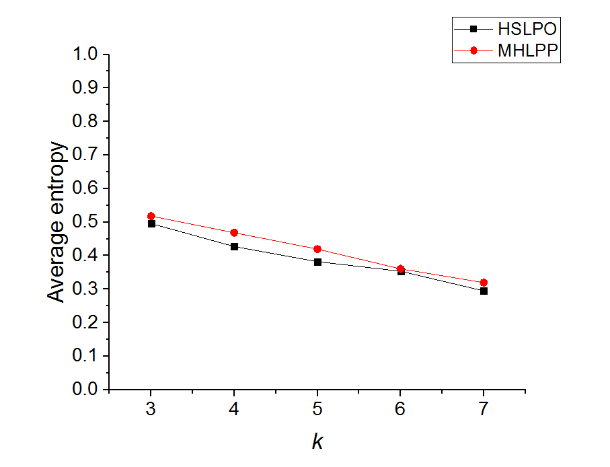
\includegraphics[width=3.0in]{figures/LPEa.png}} 
  \hspace{1in} 
  \subfigure[Locating Probability Entropy With Various Communication Radii]{ 
    \label{fig:LPE:b} %% label for second subfigure 
    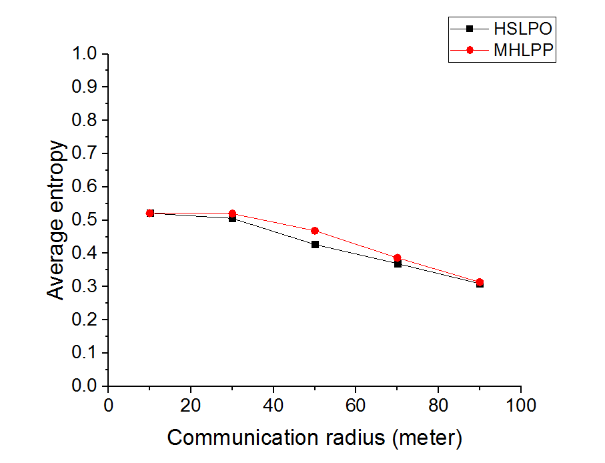
\includegraphics[width=3.0in]{figures/LPEb.png}}
  \hspace{1in} 
  \subfigure[Locating Probability Entropy With Various Privacy Thresholds]{ 
    \label{fig:LPE:c} %% label for second subfigure 
    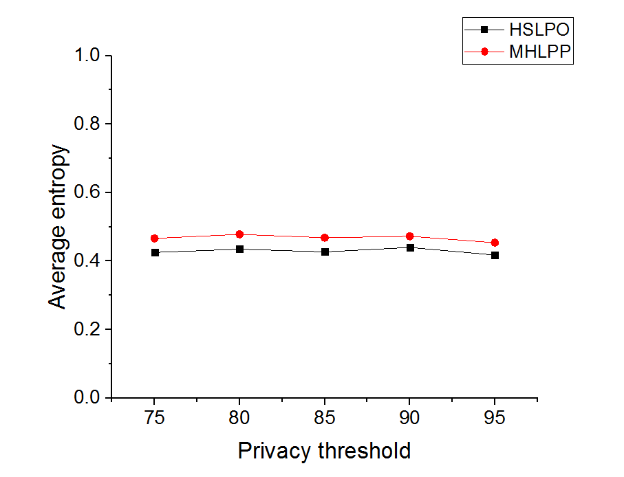
\includegraphics[width=3.0in]{figures/LPEc.png}}
  \caption{Locating Probability Entropy Comparison Between HSLPO And MHLPSP} 
  \label{fig:LPE} %% label for entire figure 
\end{figure}






%%%%%%%%%%%%%%%%%%%%%%%%%%%
\chapter{Appointment Card Protocol}
\label{CACP}
%%%%%%%%%%%%%%%%%%%%%%%%%%%
\section{System Model}

\noindent The network architecture consists of two main classes of entities: Users and Location-Based Service Providers (LBSPs). Users are mobile and communicate with other users and LBSPs within a certain range, i.e., the communication range of their portable devices. For a given user, other users in the social network are either strangers or his friends whom he can detect when they are in his communication range. Let ${RS}_{i,j}$ denote the relationship strength between user $i$ and $j$. If ${RS}_{i,j}$ is larger than a specific threshold, ${FT}_{min}$, user $j$ is considered a friend of $i$. LBSPs, which provide location-based services to the users are fixed and not part of the social network. We assume that the only information which is necessary for the LBSP is a location from the original requester, but the original requester should still give an identity (not his own) to the LBSP so that the LBSP can reply to that identity.

We consider external attacker capable of eavesdropping on limited traffic in the network. We assume that the attacker can access the database of LBSPs, so that he can learn everything recorded in LBSP's memory, including user identities and locations. The attacker launches an inference attack on each user who uses the LBS in an attempt to learn user's private information based on location and context in the queries. Therefore, the key to protecting location-privacy is degrading the relationship between the user identity and the location provided by him so that the attacker can hardly infer the identity of the original requester by the known information. 

We propose a protocol, called Appointment Card Protocol (ACP), to protect the identity and location-privacy of the original requester by providing other users' identity (agents), which can be any user in the network so that ACP can have a large anonymity set. The friends of the original requester separate the agents and the original requester so that the agents have no knowledge about the original requester.


\section{Appointment Card Protocol Overview}

\noindent Our proposed ACP protects original requesters when they are served by LBSPs. The user (${Agt}_{1}$) generates his own Appointment Cards (ACs) containing his own identity called $Cid$ and a unique number called $Capt$ (a number generated by the creator of AC). The ACs are exchanged when two users encounter each other. When the original requester sends a query, he chooses an AC and sends the query using the identity ${Agt}_{1}$ of the first agent which is in the AC. The LBSP replies to ${Agt}_{1}$ when it receives the query. ${Agt}_{1}$ is the one who has generated the AC and the first agent of the AC. ${Agt}_{1}$ then forwards the reply to the next agent (${Agt}_{2}$) who already has received AC from him, and so on until the reply reaches the last agent. The last agent is responsible for forwarding it to the original requester. Therefore, we can consider the ACP having two parts: 1) users generate and exchange ACs continuously; 2) users use ACs when they want to send a query.

\begin{figure} [H]
\centering 
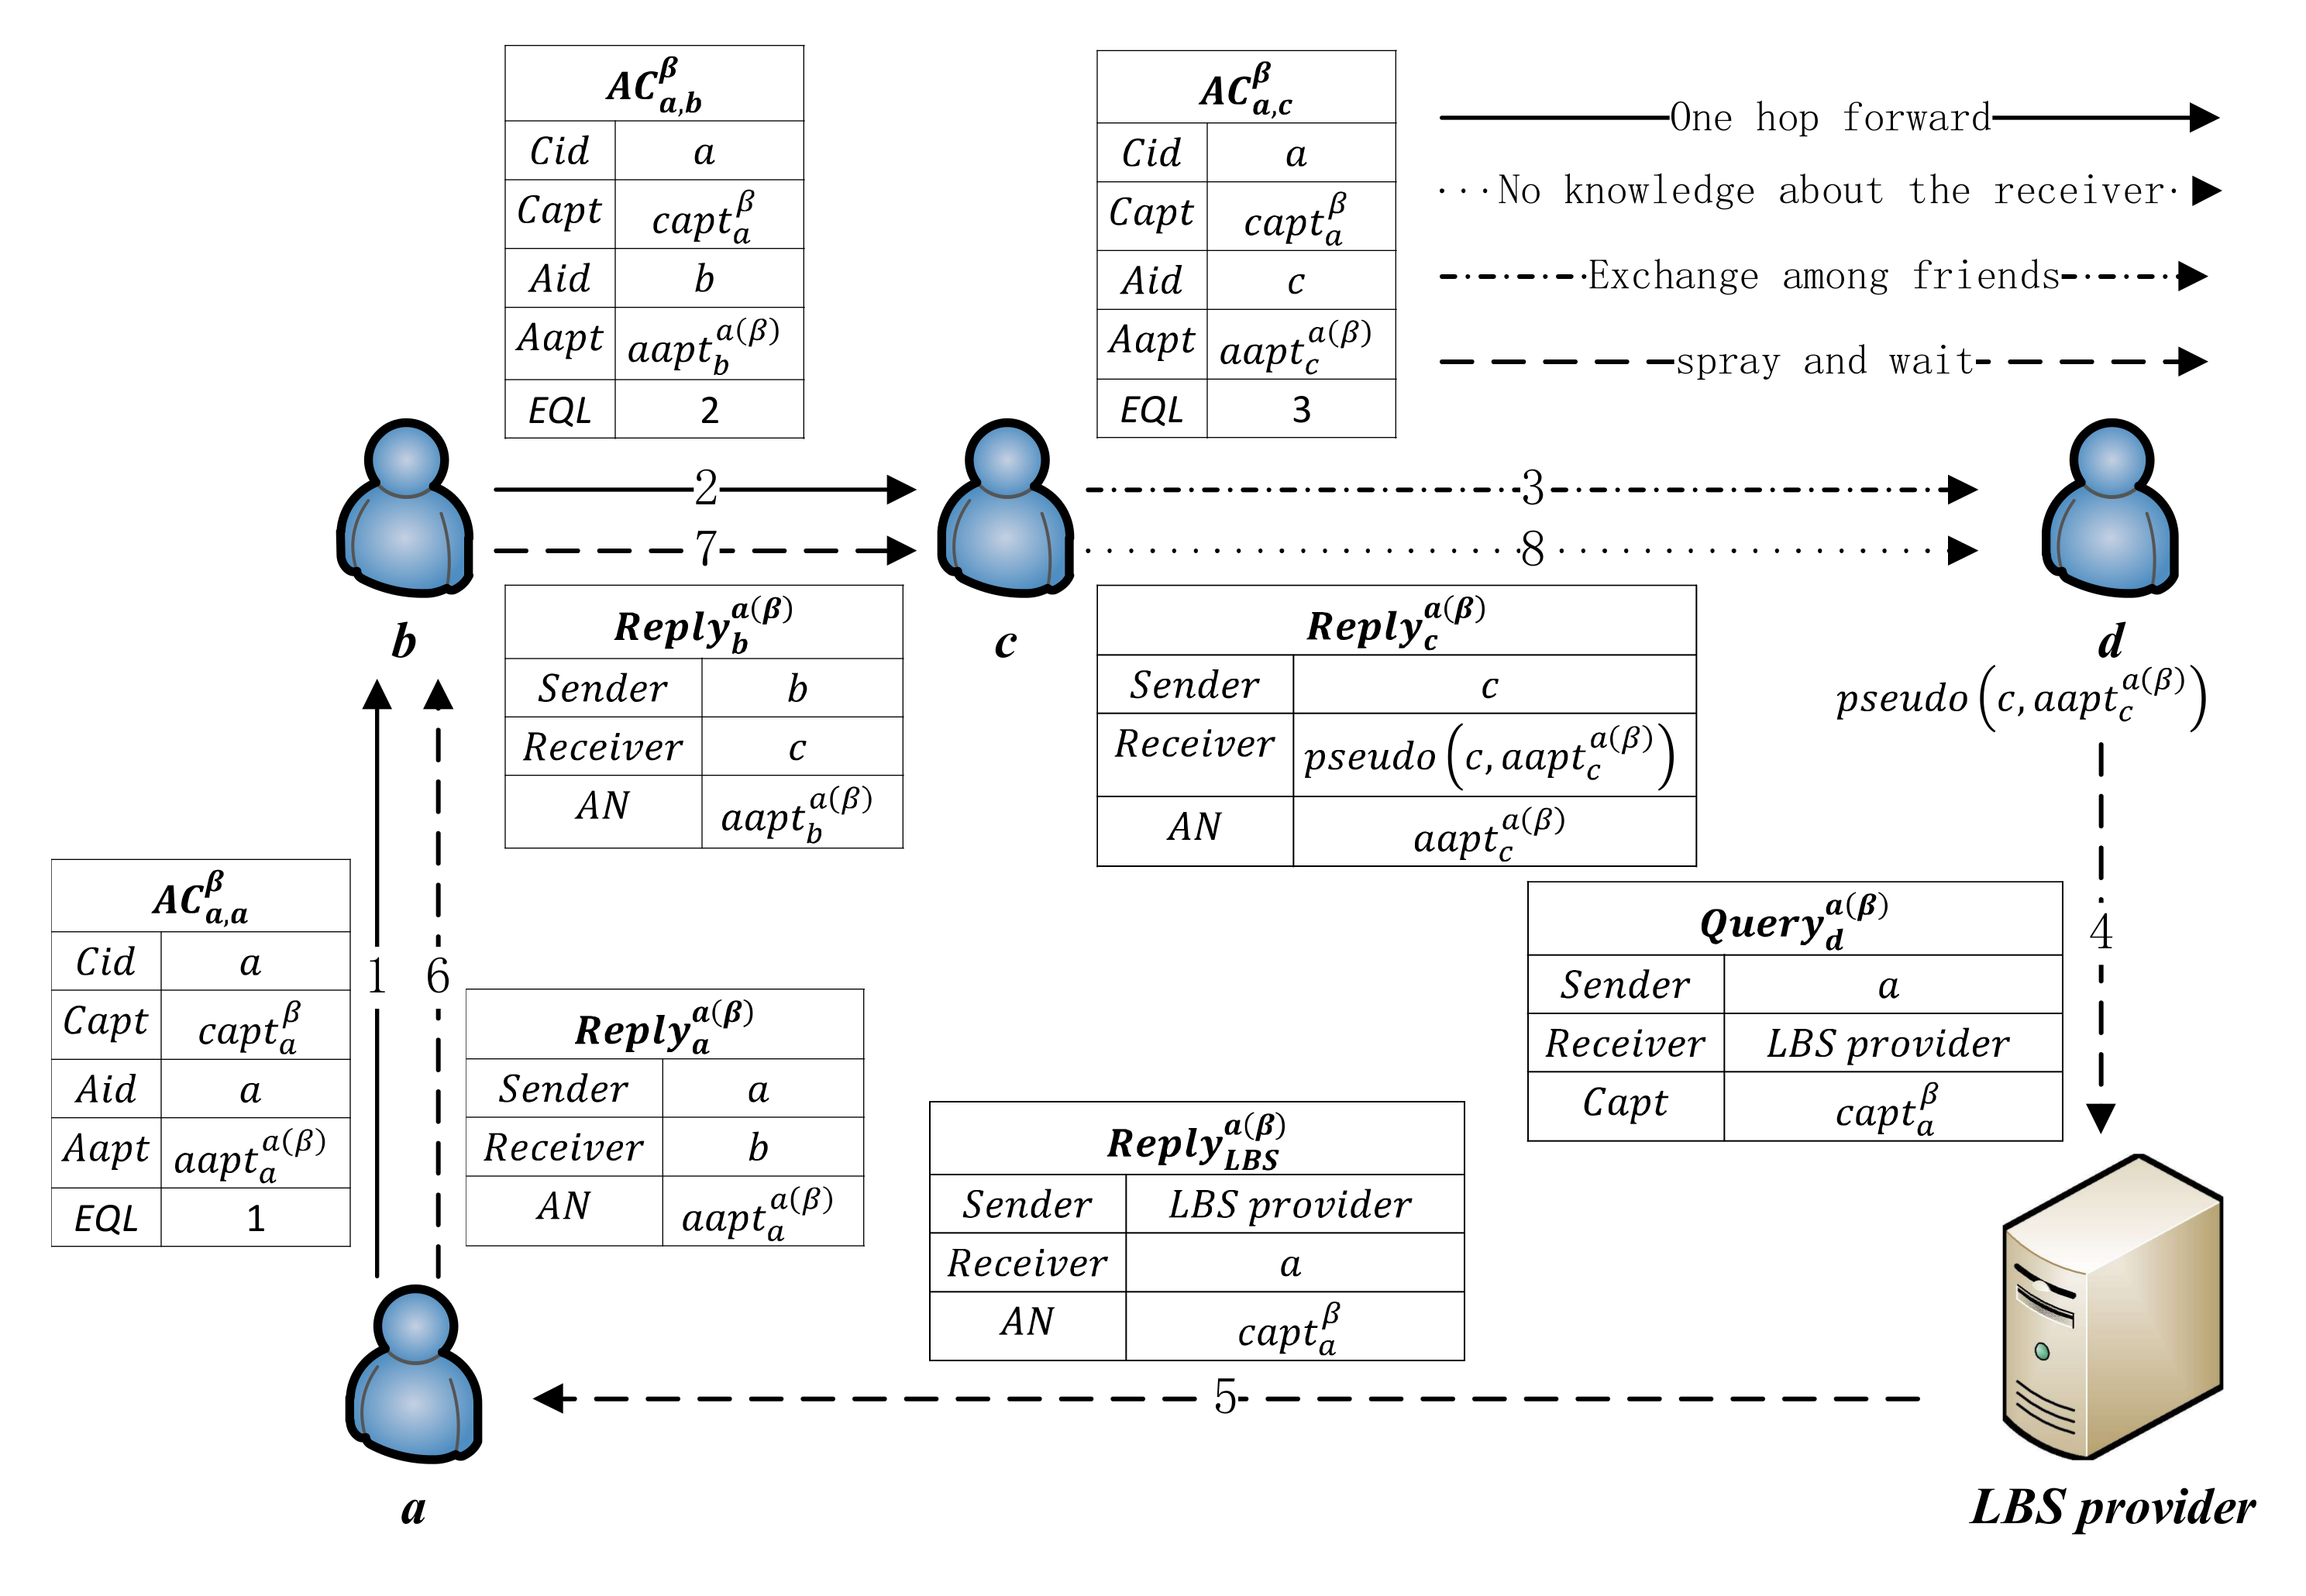
\includegraphics[width=6.0in]{figures/FIG_4_1_Example_of_ACP_Message_Exchange.png}
\caption{Example of ACP Message Exchange} 
\label{fig:EoACPME} %% label for entire figure 
\end{figure}


Figure \ref{fig:EoACPME} is an example of the execution of the ACP protocol. Explanations of the symbols in the figure are shown in Table \ref{table:ACPSymbols}. These symbols and the figure are used throughout the chapter to help us describe the protocol. For simplicity, we will omit some superscripts and subscripts from these symbols in the following sections when there is no ambiguity. The whole process can be considered as the following parts: 1) exchanging cards among all users who are called agents (i.e., 1 and 2), 2) exchanging cards among friends (i.e., 3), 3) sending query using information of appointment cards (i.e., 4), 4) forwarding the reply among agents (i.e., 5, 6 and 7), and 5) relaying to the original requester (i.e., 8). 


\begin{table} [hbtp]
\caption{ACP Symbols}
\label{table:ACPSymbols}
\centering
\tabulinesep=2mm
\begin{tabu}{|c|l|} \hline 
%\begin{tabular}{|c|l|} \hline 
Parameter & Meanings \\ \hline 
${U}_{\varepsilon}$ & An user whose identity is $\varepsilon$. \\ \hline 
${AC}_{\alpha}^{\beta}$ & The $\beta^{th}$ appointment card generated by an user $\alpha$. \\ \hline 
${AC}_{{\alpha},{\gamma}}^{\beta}$ & ${AC}_{\alpha}^{\beta}$ is being forwarded by an agent $\gamma$. \\ \hline 
${Query}_{\delta}^{{\alpha}\left({\beta}\right)}$ & A query whose original requester is $\delta$ and using ${AC}_{\alpha}^{\beta}$ \\ \hline 
${{Reply}}^{{\alpha}\left({\beta}\right)}$ & The reply of a query which uses ${AC}_{\alpha}^{\beta}$. \\ \hline 
${{Reply}}_{\gamma}^{{\alpha}\left({\beta}\right)}$ & ${Reply}^{\alpha\left(\beta\right)}$ is being forwarded by an agent $\gamma$. \\ \hline 
${{Agt}}_{i}^{{\alpha}\left({\beta}\right)}$ & The $i^{th}$ ($i\geq1$) agent of ${AC}_{\alpha}^{\beta}$. \\ \hline 
${{capt}}_{\alpha}^{\beta}$ & The parameter $Capt$ in ${AC}_\alpha^\beta$. see Table \ref{table:AptCard} \\ \hline 
${{aapt}}_{\gamma}^{{\alpha}\left({\beta}\right)}$ & The parameter $Aapt$ in ${AC}_{\alpha}^{\beta}$, which is given by an agent $\gamma$. see Table \ref{table:AptCard} \\ \hline 
$AN$ & Both the $Capt$ and the $Aapt$ in an AC are called the Appointment Number. \\ \hline 
${NR}_{\varepsilon}$ & The number of \textit{ready}-ACs carried by ${U}_{\varepsilon}$ \\ \hline 
\end{tabu}
%\end{tabular}
\end{table}

\section{Appointment Card}

\noindent To protect the original requester's location privacy, the original requester uses others' identity (${Agt}_1$) to send queries to the LBSP instead of its own identity, so that the LBSP can reply to the original requester through ${Agt}_1$. Appointment cards make it possible for the agents to forward the reply to the original requester one by one. In other words, the appointment card indicates a path through which the original requester can get its reply. 

In Figure \ref{fig:EoACPME}, the users \textit{a}, \textit{b} and \textit{c} are the agents of the appointment card ${AC}^{\beta }_a$ (i.e., ${Agt}^{a\left(\beta \right)}_1$, ${Agt}^{a\left(\beta \right)}_2$and ${Agt}^{a\left(\beta \right)}_3$). These agents are strangers, so the attackers can hardly infer $c$ from the identity of $a$. At the same time, $c$ is in the original requester $d$'s social tie (i.e.,$\ c$ is $d$'s friend or his friends' friend, so on), and he is the only one who knows how to reach $d$. Therefore, it is hard for attackers to infer the identity of $d$ from the identity of $a$.

Notice that $c$ receives $a$'s appointment card (i.e. ${AC}^{\beta }_a$) from a stranger $b$ who knows the information of ${AC}^{\beta }_a$ and the identity of the next agent $c$, so that it is unsafe for $c$ to use that appointment card. In other words, the appointment card cannot be used until $c$ exchanges it with another user (e.g., the user $d$) who trusts $c$. The appointment card is called a \textit{ready appointment card} (\textit{ready}-AC) after it leaves the last agent (i.e., the user $c$), or it is called the \textit{distributing appointment card} (simply \textit{distributing}-AC). It is obvious that \textit{distributing}-ACs are transmitted among agents who can be strangers, while an user can only get \textit{ready}-ACs from one of his friends.

To make users carry a similar number of \textit{ready}-ACs, \textit{ready}-ACs are also exchanged between friends, so that an user can get \textit{ready}-ACs from his friends who have more \textit{ready}-ACs than him. As a result, the last agent is not sure whether the user who gets the \textit{ready}-AC from him is the original requester. We introduce a pseudonym mechanism which enables the last agent to forward the reply to the unknown original requester. 

All users in the network are responsible for generating their respective ACs, and they are called the creators of their own ACs. The creator records his own identity ($Cid$) and a unique number ($Capt$) on his AC. When users exchange ACs, they modify $Aid$ (the agent ID) and ${Aapt}$ (the agent's appointment number) in the AC to enable the next agent to identify who is the predecessor. Entries of AC are shown in Table \ref{table:AptCard}.


\begin{table} [hbtp]
\caption{Appointment Card}
\label{table:AptCard}
\centering
\tabulinesep=2mm
\begin{tabu} to 140 mm {|X[1,c]|X[4,l]|} \hline 
%\begin{tabular}{|c|l|} \hline 
Parameter & Meanings \\ \hline 
$Cid$ & The identity of the creator who generates the AC. \\ \hline 
$Capt$ & A unique number that distinguishes an AC from other ones generated by the same creator. \\ \hline 
$Aid$ & The identity of an agent who gives the AC to the recent holder. (The previous hop of the AC) \\ \hline 
$Aapt$ & A unique number that distinguishes an AC from other ones transmitted by the same agent. \\ \hline 
$Timeout$ & The time when the AC expires. \\ \hline 
\textit{EQ} & A queue (Exchange Queue) which records users who exchange the AC in order. Its length is \textit{EQL}. \\ \hline 
\end{tabu}
%\end{tabular}
\end{table}


\section{AC Life Cycle}

\noindent The life cycle of an AC starts when it is generated by its creator. The first $k$ (see Table \ref{table:ImptACSysParam}) agents add their identities into its Exchange Queue (\textit{EQ}) (see Table \ref{table:AptCard}) before exchanging it, which increases the length (\textit{EQL}) of the \textit{EQ}. When the AC's \textit{EQL} reaches $k$, it is eligible to be used in a query and is called a \textit{ready }AC. When an AC is used in a query, it is marked as an \textit{used} AC by the original requester who uses the AC. An AC starts at the \textit{distributing} state. No matter what state (\textit{distributing}, \textit{ready} or \textit{used}) an AC is in, it can expire, as shown in Figure \ref{fig:ACLifeCycle}. If the length of its \textit{EQ} reaches \textit{k}, it is switched to the \textit{ready} state. It can timeout in all states. When an user uses a \textit{ready} AC in a query, the AC is switched to the \textit{used} state. The user can also use the \textit{used} AC in other queries but he does not give the AC to anyone else. 

\begin{figure} [hbtp]
\centering 
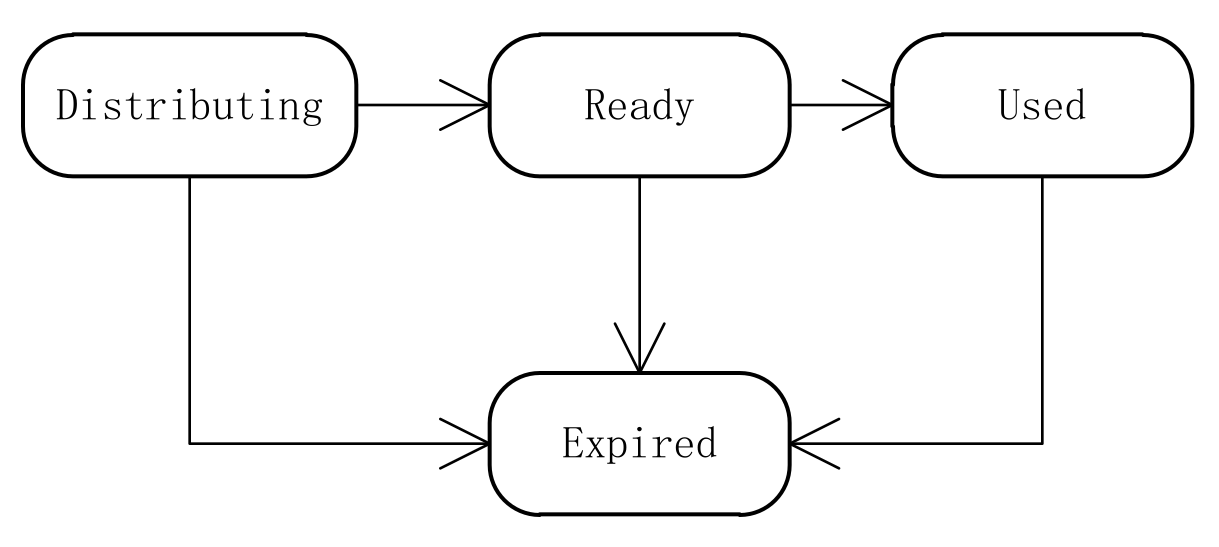
\includegraphics[width=4.0in]{figures/aclifecycle.png}
\caption{AC's Life Cycle} 
\label{fig:ACLifeCycle} %% label for entire figure 
\end{figure}

\section{System Parameters}

\noindent All the system parameters are shown in Table \ref{table:ImptACSysParam}. 

\begin{table} [hbtp]
\caption{Important System Parameters}
\label{table:ImptACSysParam}
\centering
\tabulinesep=2mm
\begin{tabu} to 110 mm {|X[1,c]|X[4,l]|} \hline 
%\begin{tabular}{|c|l|} \hline 
Parameter & Meanings \\ \hline 
$k$ & The obfuscation distance \\ \hline 
$m$ & The friend obfuscation distance \\ \hline 
$GP$ & The generating period of appointment cards \\ \hline 
$Seg$ & The distributing segment \\ \hline 
$\tau$ & Avoiding time \\ \hline 
$AT$ & The timeout for appointment cards \\ \hline 
\end{tabu}
%\end{tabular}
\end{table}

\subsection{Obfuscation Distance}

\noindent The obfuscation distance $k$ is the number of exchange before an AC is switched to the \textit{ready} state. In other words, an AC must be exchanged $k$ times before it becomes a \textit{ready}-AC which can be used by an user in queries.

As shown in Figure \ref{fig:ObfuscationDistance}, the first $k-1$ agents are strangers so that the only relationship between two adjacent ones is that they encounter each other somewhere. The relationship between ${Agt}_1$ and ${Agt}_k$ becomes weaker when we increase $k$. In other words, attackers can hardly infer the identity of ${Agt}_k$ when they only knows the identity of ${Agt}_1$, and the difficulty increases with the increase of parameter $k$. As a result, it is hard for attackers to infer the original requester, even though ${Agt}_k$ is in the social tie of the original requester. Since the reply message must go through a series of agents, a long obfuscation distance also lengthens the path of the reply message. Therefore, a large $k$ makes the original requester safer, while making it harder and longer for the reply to be delivered.

\begin{figure} [hbtp]
\centering 
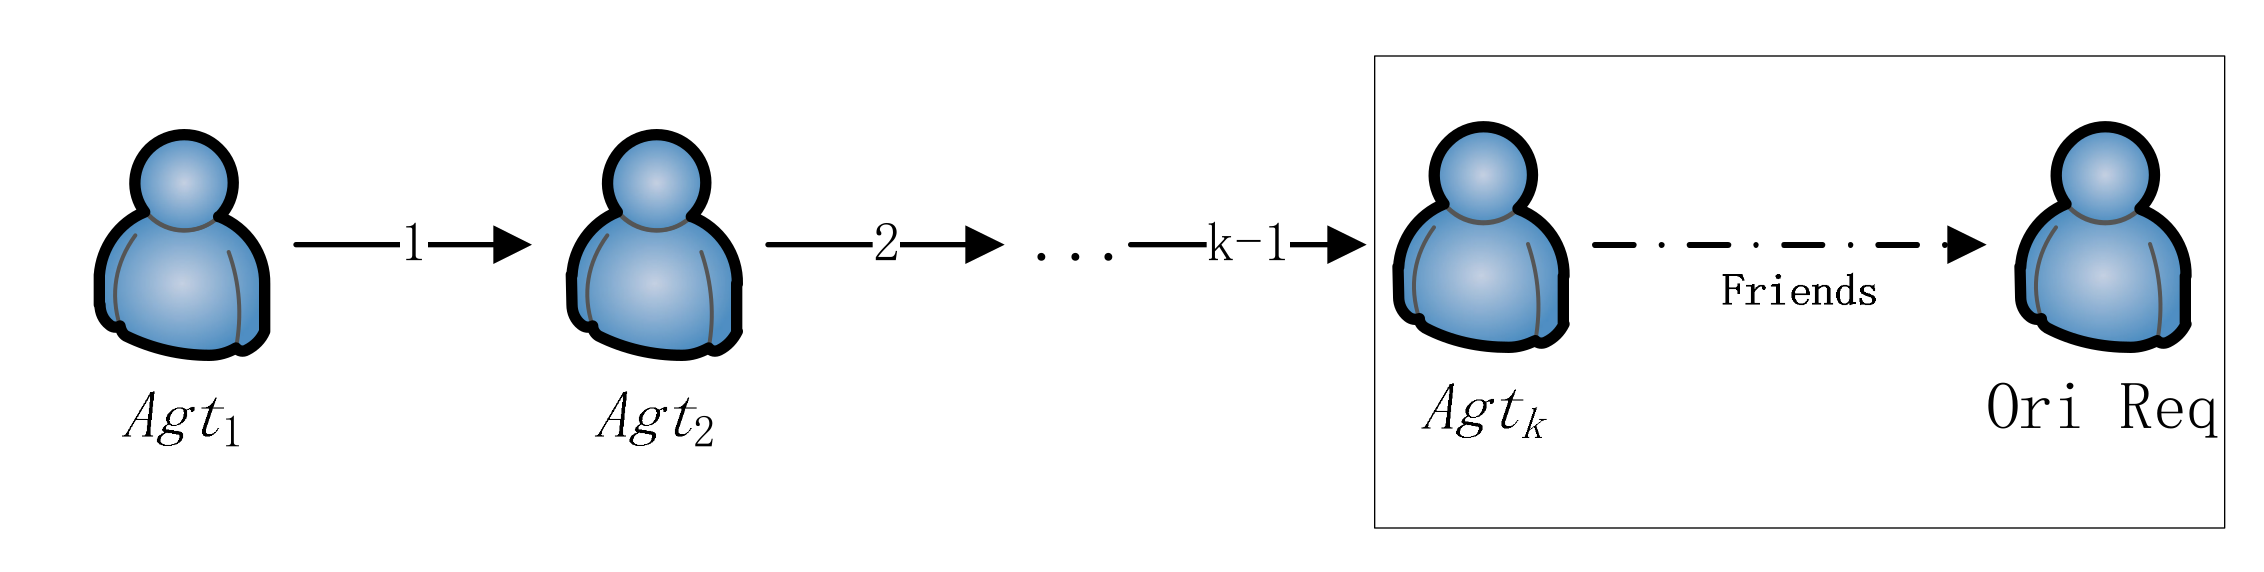
\includegraphics[width=6.0in]{figures/ACPObfDis.png}
\caption{Obfuscation Distance} 
\label{fig:ObfuscationDistance} %% label for entire figure 
\end{figure}

\subsection{Friends Obfuscation Distance}

\noindent Since ${Agt}_{k-1}$ is a stranger for ${Agt}_k$, it is possible that ${Agt}_{k-1}$ is the attacker. We assume that the attacker knows that ${Agt}_k$ is in the social tie of the original requester. The attacker can assume that ${Agt}_k$ is a close friend of the original requester, so the identity of ${Agt}_k$ gives the attacker a good tip to infer the original requester. A solution to prevent the agent ${Agt}_{k-1}$ from learning the identity of the original requester easily is that the last $m$ ($1\leq m\leq k$) agents are friends, as shown in Figure \ref{fig:FriObfuscationDistance}. Here, $m$ is called \textit{friends obfuscation distance}, and the last $m$ agents are trusted agents.

\begin{figure} [hbtp]
\centering 
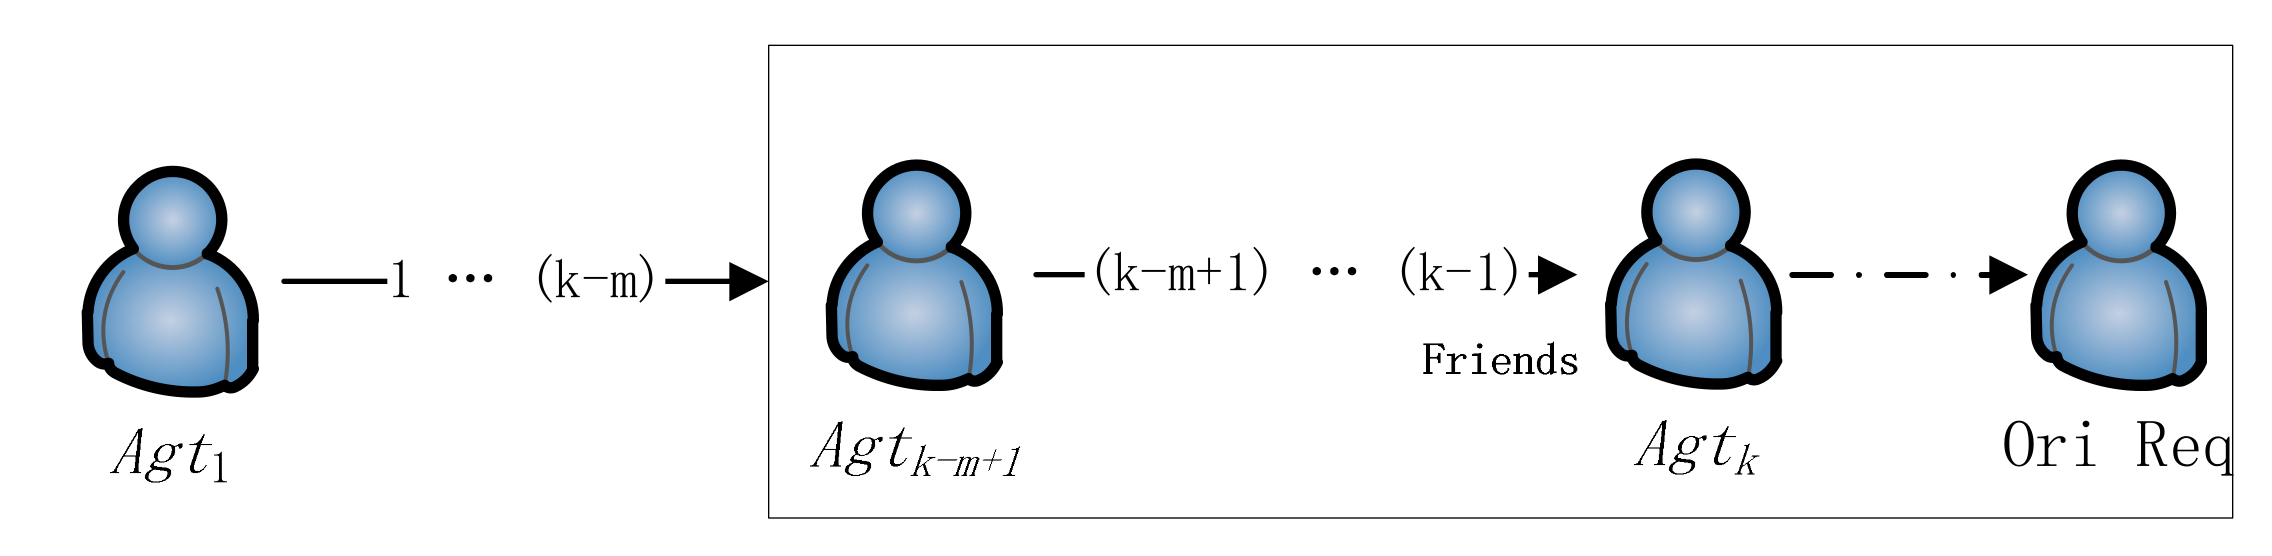
\includegraphics[width=6.0in]{figures/ACPFriObfDis.png}
\caption{Friends-Obfuscation Distance} 
\label{fig:FriObfuscationDistance} %% label for entire figure 
\end{figure}

It is true that ${Agt}_i$ is a friend of ${Agt}_{i+1}$, $i>k-m$, but two nonadjacent trusted agents (e.g., ${Agt}_i$ and ${Agt}_{i+2}$) might have a weak relationship. Since there are at least $m$ trusted agents between the stranger ${Agt}_{k-m}$ and the original requester, ${Agt}_{k-m}$ can hardly infer the identity of the original requester based on information he learns. When $m=k$, all ACs must be exchanged between friends only. When $m=1$, the last agent is the only one who is in social tie of the original requester, which is the case in our example.

However, friends encounter each other rarely, so having a large \textit{m} increases the difficulty of distributing ACs. In this work, we assign $m$ to 1.

\subsection{Generating Period}

\noindent Since ACs could expire, users must generate new ACs continuously. We use $GP$ to denote the speed of generating new ACs per user; that is, each user generates a new AC every $GP$ seconds.



\subsection{Distributing Segment}

\noindent It is the series of random agents that increases the difficulty for attackers to infer the identity of the original requester. However, it is possible that many ACs are transmitted by the same series of agents. We use the system parameter distributing segment, $Seg$, to avoid giving all \textit{distributing}-ACs to the same user. Each user maintains $Seg$ number of \textit{Distributing AC List}s (\textit{DL}s). It puts received \textit{distributing}-ACs in one of those \textit{DL}s randomly. If ${Agt}_i$ exchanges ACs with another user, ${Agt}_i$ selects one of his \textit{DL}s, and only ACs in that \textit{DL} will be exchanged with that user.

For example, we assign $Seg=2$ so that each user has two \textit{DL}s (i.e., \textit{DL}1 and \textit{DL}2). When $U_b$ receives ${AC}^1_{a,a}$, ${AC}^2_{a,a}$ and ${AC}^3_{a,a}$ from $U_a$, $U_b$ may put ${AC}^1_{a,a}$ and ${AC}^2_{a,a}$ in its \textit{DL}1, while ${AC}^3_{a,a}$ in its \textit{DL}2. If $U_b$ encounters $U_c$, $U_b$ can give either ${AC}^1_{a,b}$ and ${AC}^2_{a,b}$ or only ${AC}^3_{a,b}$ to $U_c$. In this way, we separate ACs generated by the same creator.

\subsection{Avoiding Time} \label{subsubsecAvdTime}

Duplicated agents make the obfuscation path of an AC less complicated. We use a parameter \textit{avoiding time,} $\tau$, to optimize the agent selection strategy. If an user gets an \textit{distributing}-AC at time $t_i$, he cannot get that \textit{distributing}-AC again before time $t_i+\tau $.

\subsection{AC Timeout}

\noindent Let $AT$ denote the timeout of ACs. An AC expires $AT$ seconds after it is generated. When an AC expires, all agents delete the AC information from their memory.

\section{Protocol Details}


\subsection{Generating Appointment Cards}

\noindent Maintaining a certain number of ACs in the network is a prerequisite for users for sending queries. Considering that ACs can expire, users must generate ACs continuously. The user who generates an AC is called the creator of the AC; at the same time, he is also the first agent of the AC. ACs are created based on two principles: fairness and continuity. 

ACs impose a burden on agents. In fact, agents are unlikely to benefit from relaying messages to the original requester because they need to allocate memory to save ACs' information, and they consume energy to forward replies. To prevent users who generate more ACs than others from being overloaded, some fairness mechanism must be in place to ensure that all users generate a relatively equal number of ACs.

We assume that the AC timeout (i.e., $AT$) is 30 minutes, and every user generates 100 ACs at the beginning and generates no AC until the 30${}^{th}$ minute. Since all agents remove the information of expired ACs from their memory, they can hardly deliver replies which use expired ACs. As a result, it is hard for an user to select an appropriate AC for his query at the 29${}^{th}$ minute when all ACs only have 1 ($=30-29$) more minute, because agents may not be able to forward the reply of his query even though the LBS receives the query successfully. Therefore, the generating strategy should be steady and sustainable.

In our protocol, each user generates a new AC every $GP$ second. Since an AC has an $AT$-seconds timeout, there are $\delta =\frac{AT}{GP}$ appointment cards held by each user in the network. In other words, each user maintains about $\delta$ ACs which is generated by himself, and we meet the fairness criteria. Since users create ACs continuously, ACs have various timeouts so that it is likely for an user to pick an AC which does not expire in a long time (at least longer than his queries and replies).


\subsection{Exchange Distributing Appointment Cards}\label{subsec_ExchangeDisAptCrd}

\noindent Users exchange their \textit{distributing}-ACs as frequently as possible, so that a \textit{distributing}-AC can be switched to a \textit{ready} one quickly. Still, there are some other conditions which should be satisfied when exchanging a \textit{distributing}-AC. Users should avoid giving all their \textit{ready}-ACs to a single user, which leads to identical set of AC agents. As shown in subsection \ref{subsubsecDisSeg}, we use $Seg$ and \textit{DL}s to separate \textit{distributing}-ACs. We also need to prevent ACs from having duplicated agents using $\tau$ which is described in subsection \ref{subsubsecAvdTime}.

We assume that two users, e.g., $U_A$ and $U_B$, are walking together for a period. Also assume that $U_A$ generates an AC (e.g., ${AC}_A$) at $t_0$ and exchanges it to $U_B$, then ${AC}_A$ is given back to A and so on. The distributing phase of the AC only costs a few seconds, because $U_A$ and $U_B$ exchange ${AC}_A$ time and again, but they are the only agents involved. The above scenario defeats the purpose of exchanging ACs because it is easy for an attacker to infer the last agent who may be $U_A$ or $U_B$ from the first agent $U_A$. We can prevent an AC from having repeated agents when using the parameter $\tau$. For example, $U_B$ receives a certain AC ${AC}_A$ from $U_A$ at $t_0$, then $U_B$ sends it to an user C ($U_C$) who can also send it to others. If an user carrying ${AC}_A$ encounters $U_B$ before $t_0+\tau $, he cannot send ${AC}_A$ to $U_B$. Therefore, if the parameter $\tau $ is larger than or equal to the parameter \textit{AT}, there is no repeated agent in an AC's \textit{EQ}. In other words, an AC never reaches an agent twice when $\tau $ is equal to \textit{AT}. In this thesis, we assign $\tau $ to \textit{AT}. 

Besides, we should also avoid ACs having the same series of agents, as we mention in the distributing segment subsection. Now we propose the strategy of exchanging \textit{distributing}-ACs.

Let us take a pair of users Alice and Bob as an example. If Alice encounters another user Bob, Bob tells Alice whether he trusts her (Bob views her as a friend). Alice picks one of her \textit{distributing}-AC lists (e.g., \textit{DL}1). Alice traverses all ACs in \textit{DL}1 and \textit{distributing}-ACs which satisfy the following two conditions before exchanging them with Bob:

\begin{enumerate}
\item If the length of the AC's \textit{EQ} (i.e., \textit{EQL}) is not shorter than $k-m$, then Alice must be a friend of Bob.

\item Bob was not carrying the AC in the recent $\tau $ time interval.
\end{enumerate}

When Alice sends a \textit{distributing}-AC to Bob, she adds her identity and the current time to the AC's \textit{EQ}. Besides, Alice must modify the AC's $Aid\mathrm{\ }$to her own identity and its $Aapt$ to a new one. She also records the information in Table \ref{table:RelayTableEntries} as \textit{relay-table} in her memory. We should notice that the first agent (i.e., the creator) does not have a ${Aapt}_{old}$, because he is precisely the one who has generated the AC, in which case the ${Aapt}_{old}$ indicates his own identity. When Bob gets those ACs, he puts each one of the received \textit{distributing}-ACs in his \textit{DL}s respectively and randomly. If an AC whose \textit{EQL} is already equal to $k$, the AC must be switched to a \textit{ready} state when Bob gets it. Bob puts \textit{ready}-ACs in his \textit{ready}-AC list instead of \textit{distributing}-AC lists.

\begin{table} [hbtp]
\caption{Relay Table Entries}
\label{table:RelayTableEntries}
\centering
\tabulinesep=2mm
\begin{tabu} to 110 mm {|X[1,c]|X[4,l]|} \hline 
%\begin{tabular}{|c|l|} \hline 
Parameter & Meanings \\ \hline 
${Aapt}_{old}$ & The $Aapt$ generated by the previous agent \\ \hline 
${Aid}_{old}$ & The identity of the previous agent \\ \hline 
${Aapt}_{new}$ & The new $Aapt$ (generated by himself) \\ \hline 
${ID}_{nxt}$ & The identity of the next agent \\ \hline 
\textit{EQL} & The length of the AC's \textit{EQ} (should larger than 0) \\ \hline 
$AT$ & The time when the AC times out. \\ \hline 
\end{tabu}
%\end{tabular}
\end{table}

\subsection{Exchange Ready Appointment Cards}

\noindent Users ask for \textit{ready}-ACs only from their friends, which prevents strangers from learning the information of the users who are holding the \textit{ready}-ACs. The strategy of exchanging \textit{ready}-ACs should also meet some fairness criteria. That is, the number of each user's \textit{ready}-ACs should be more or less equal. 

Let us consider two friends Alice and Bob as an example. Alice has 20 ACs, while Bob has 10 ACs. When they encounter each other, it is reasonable that they both give half of their \textit{ready}-ACs to the other. As a result, they both will have half of the total (15) ACs. However, that strategy does not work all the time as explained below.

The problem becomes more complex in the following condition. Alice is a friend of Bob, while Bob is not a friend of Alice. In other words, Bob trusts Alice, but Alice does not trust Bob. We assume that Alice is a trusted but suspicious girl so that many users trust her while she trusts few users while Bob is opposite. When users encounter Alice, they ask for \textit{ready}-ACs from her, but Alice rarely asks for \textit{ready}-ACs. Therefore, Alice carries few \textit{ready}-ACs, while Bob carries many \textit{ready}-ACs. When Alice and Bob encounter each other, and Bob asks for \textit{ready}-ACs, then the strategy seems unfair for Alice. To ensure the fairness and the efficiency of the strategy, users must compare the number of their own \textit{ready}-ACs and the number of \textit{ready}-ACs carried by the other user when two users are exchanging \textit{ready}-ACs.

When Bob encounters Alice, Bob tells Alice the number of his \textit{ready}-ACs (${NR}_{Bob}$) and whether he wants Alice's \textit{ready}-ACs (if he trusts Alice). If Alice learns that Bob needs her \textit{ready}-ACs, she compares the number of her \textit{ready}-ACs (${NR}_{Alice}$) and ${NR}_{Bob}$. If ${NR}_{Bob}\ge {NR}_{Alice}$, Alice gives no \textit{ready}-AC to Bob; otherwise, she gives $\frac{{NR}_{Alice}-{NR}_{Bob}}{2}$ to Bob. In this way, \textit{ready}-ACs do not concentrate in a group of users who trust many users. 

The process of exchanging \textit{ready}-ACs is much more straightforward than that for \textit{distributing}-ACs. Users do not modify any information in the \textit{ready}-ACs including $Aapt$ and $Aid$ so that the parameters of \textit{ready}-ACs always stay the same.

The algorithm of exchanging ACs when an user $U_i$ encounters another user $U_j$ is shown in Algorithm \ref{AlgExchACs}. The two users tell each other whether they are friends at the very beginning of their encounter. After they both know their relationship, they start to exchange their \textit{distributing}-ACs. When they both finish receiving the \textit{distributing}-ACs from the other, they continue to exchange their \textit{ready}-ACs at the same time. The process ends when they finish exchanging their \textit{ready}-ACs (or they do not need to exchange \textit{ready}-ACs).

\begin{algorithm} [hbtp]
\caption{Algorithm for exchanging ACs}\label{AlgExchACs}
\begin{algorithmic}[1]
\Procedure {Encounter} {$U_j$}
\If {$U_i$ trusts $U_j$}
\State $U_i$ tells $U_j$ that $U_j$ is viewed as a friend.
\Else
\State $U_i$ tells $U_j$ that $U_j$ is not viewed as a friend.
\EndIf
\State Wait for $U_j$ to tell $U_i$ whether $U_i$ is viewed as a friend.
\State $U_i$ chooses a distributing list (${DL}_{\omega}$) randomly.
\For {each ${AC}_u$ in ${DL}_{\omega}$}
\If {$U_j$ was carrying ${AC}_u$ in the recent $\tau$ time}
\State ${AC}_u$ cannot be sent to $U_j$
\State continue (Try the next one.)
\EndIf
\If {the \textit{EQL} of ${AC}_u$ $\geq$ $k-m$}
\If {$U_i$ is not trusted by $U_j$}
\State ${AC}_u$ cannot be sent to $U_j$
\State continue (Try the next one.)
\EndIf
\EndIf
\State Send ${AC}_u$ to $U_j$
\EndFor
\State Tell $U_j$ that all \textit{distributing}-ACs are sent.
\State Receive all \textit{distributing}-ACs from $U_j$
\If {$U_i$ trusts $U_j$}
\State $U_i$ tells $U_j$ ${NR}_i$.
\EndIf
\If {$U_i$ is trusted by $U_j$}
\State Wait for $U_j$ to tell $U_i$ ${NR}_j$.
\If {${NR}_j\geq{NR}_i$}
\State send no \textit{ready}-AC to $U_j$
\Else
\State send $\frac{{NR}_i-{NR}_j}{2}$ number of \textit{ready}-ACs to $U_j$
\EndIf
\State Tell $U_j$ all \textit{ready}-ACs are sent.
\EndIf
\If {$U_i$ trusts $U_j$}
\State Wait for \textit{ready}-ACs from $U_j$.
\EndIf 
\EndProcedure

\end{algorithmic}
\end{algorithm}

\subsection{Sending Queries}

\noindent The original requester must be able to send his queries to the LBSP and be able to get the reply while preventing the LBSP from learning his identity. In ACP, the original requester sends his query using $Agt_1$'s identity to the LBSP, and $Agt_1$ is responsible for forwarding the reply from LBSP to the original requester. Therefore, the original requester's query includes a sender identity ${Agt}_1$, which is equal to the $Cid$ in the AC. Since ${Agt}_1$ needs a ${Capt}$ to identify the AC used by the query (and the reply), the ${Capt}$ in the AC is also in the query. The network can deliver that query to the destination LBSP efficiently with any DTN protocol.

We use the example in Figure \ref{fig:EoACPME}. The original requester $U_d$ has an AC (i.e., ${AC}^{\beta }_{a,c}$) whose creator is $U_a$. When $U_d$ uses it to send his query ${Query}^{a\left(\beta\right)}_d$, the sender identity is $a$, and the $Capt$ of the query is the $Capt$ of ${AC}^{\beta }_{a,c}$, as shown in Figure \ref{fig:ConstituteQuery}.

\begin{figure} [H]
\centering 
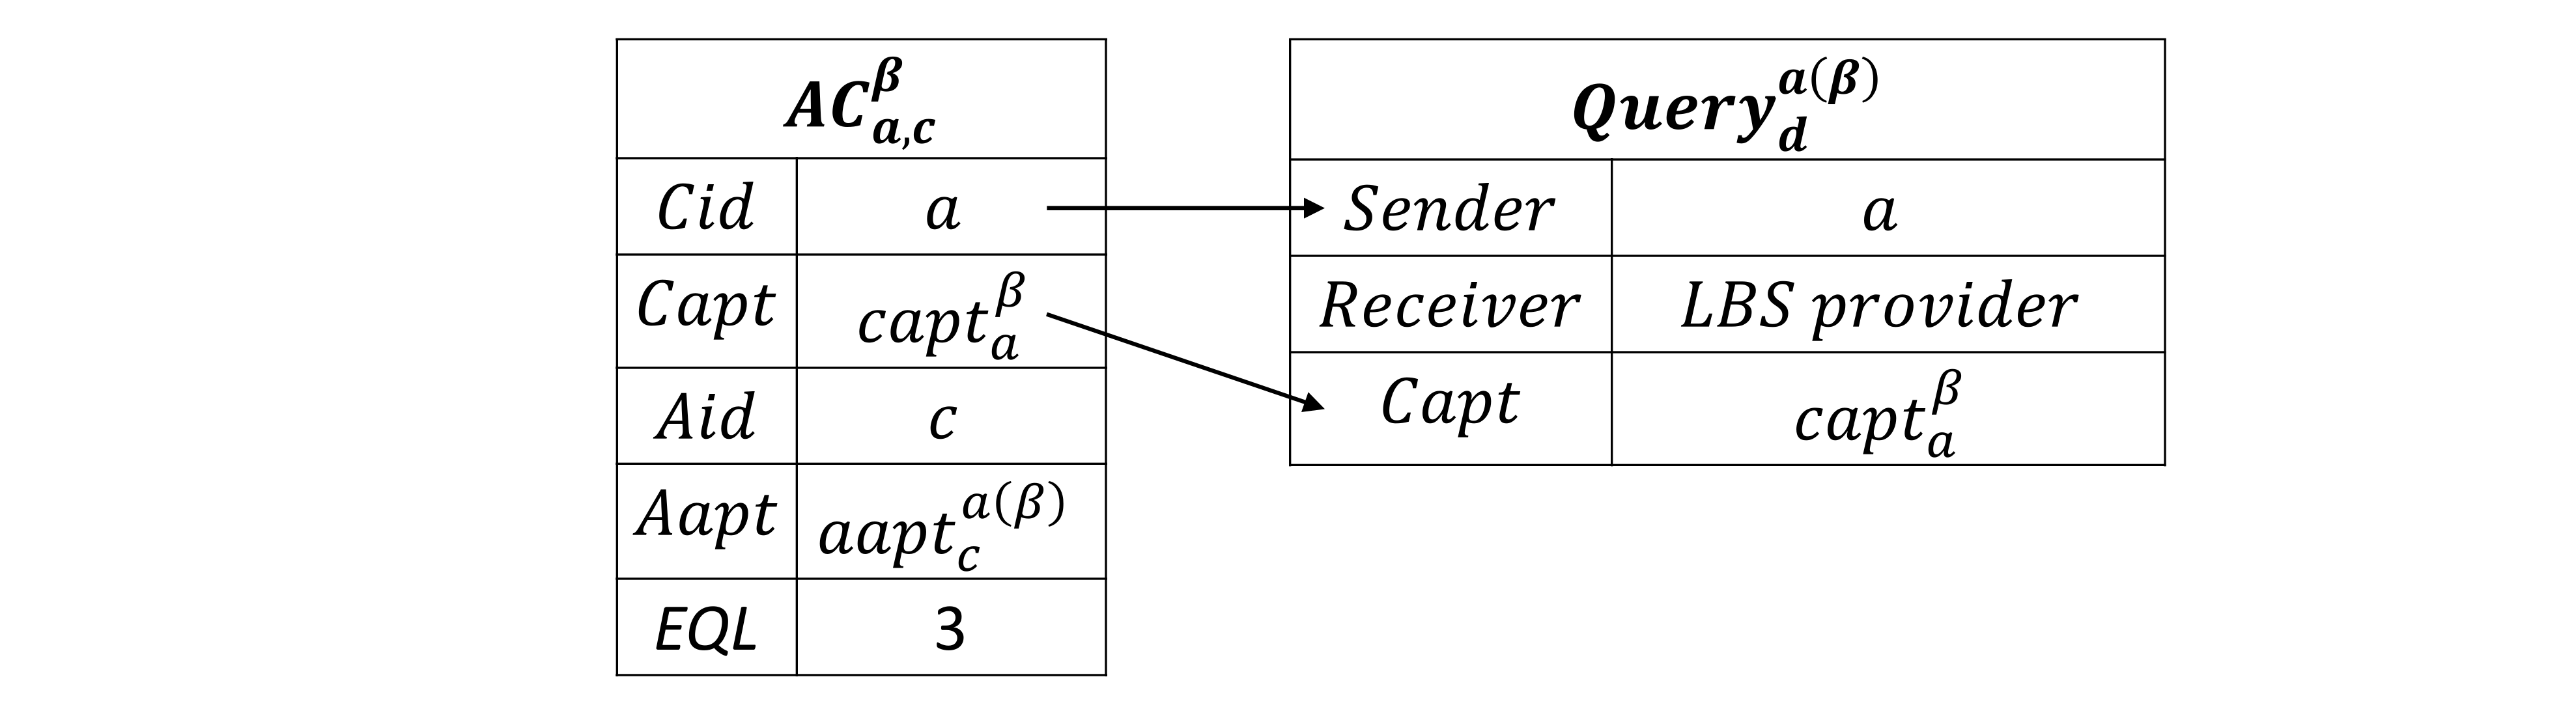
\includegraphics[width=6.0in]{figures/FIG_4_5_Constitute_Query.png}
\caption{Constitute Query} 
\label{fig:ConstituteQuery} %% label for entire figure 
\end{figure}

The AC is marked as used when the query is ready to be sent so that the AC cannot be exchanged with other users. The original requester also uses a pseudonym to receive the reply, which is described in subsection \ref{paraLastAgent}. The algorithm that an user $U_i$ uses to send a query is shown in Algorithm \ref{AlgSendACPQuery}.


\begin{algorithm} [hbtp]
\caption{Algorithm for Sending Queries}\label{AlgSendACPQuery}
\begin{algorithmic}[1]
\Procedure {SendQuery } {}
\State Choose an \textit{ready}-AC, say ${AC}_{\alpha,f}^{\beta}$.
\State Assign the sender identity of the query to $U_{\alpha}$
\State Assign the receiver identity to the LBS
\State Assign the $AN$ to the ${capt}_{\alpha}^{\beta}$
\State Get a pseudonym $pseudo\left(U_f,{aapt}_f^{\alpha \left(\beta \right)}\right)$
\State Use the pseudonym as $U_i$’s identity.
\State Send the query to the LBS.
\EndProcedure
\end{algorithmic}
\end{algorithm}

\subsection{Sending Replies}


\subsubsection{The LBSP part}

\noindent When the LBSP receives the query, it learns that the sender's identity is the first agent $U_a$ instead of the original requester $U_d$, which protects the location privacy of the original requester. In Figure \ref{fig:ConstituteReplies}, the LBS provider replies to the sender $U_a$, when it receives ${Query}^{a\left(\beta\right)}_d$. The reply also includes the $Capt$ of the query (i.e., $capt_a^\beta$), which enables $U_a$ to identify the AC used in the query and the reply.

\begin{figure} [H]
\centering 
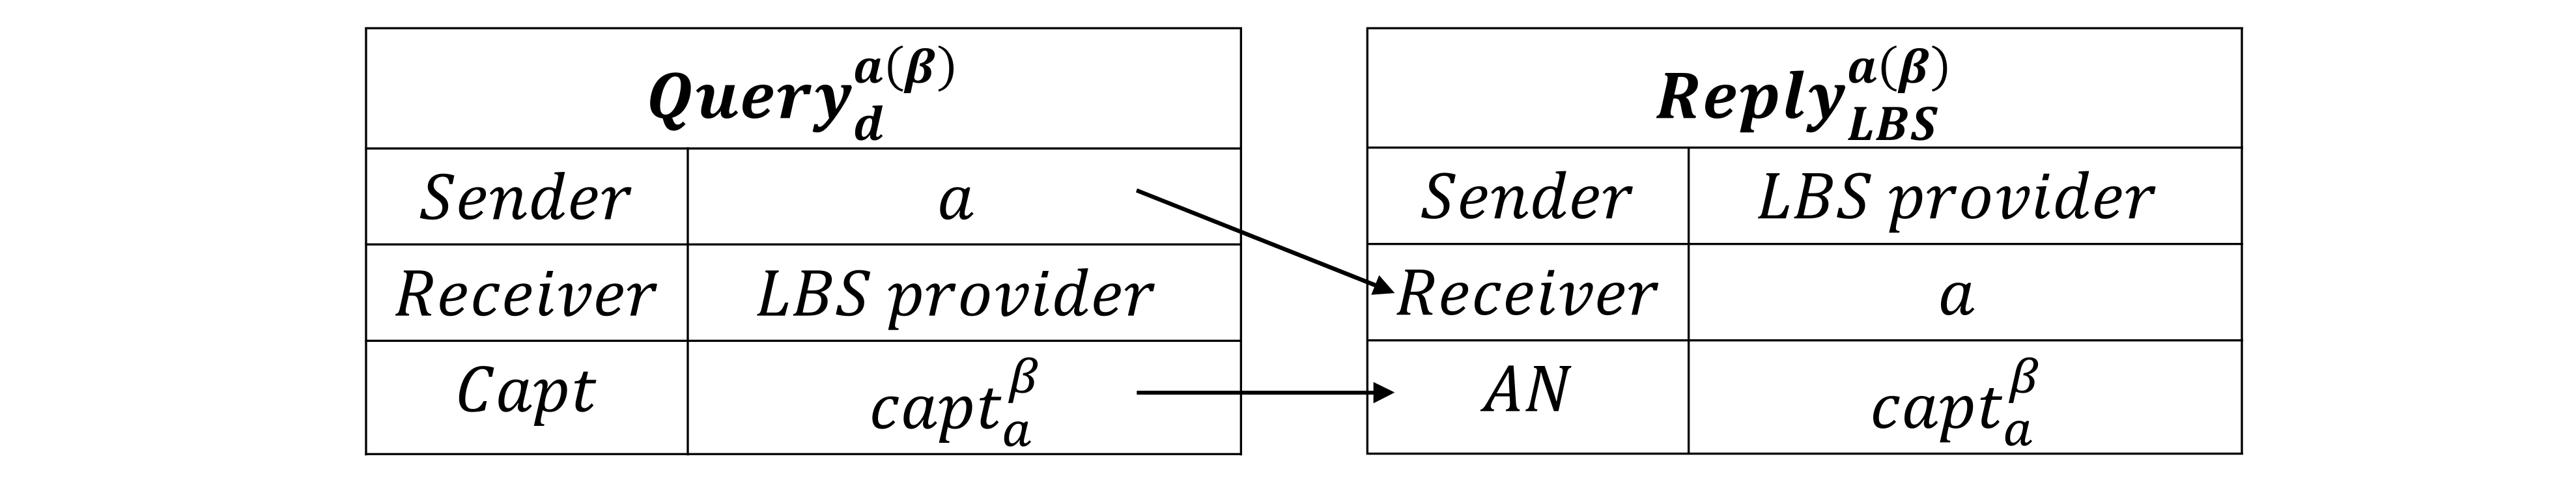
\includegraphics[width=6.0in]{figures/FIG_4_6_Constitute_Replies.png}
\caption{Constitute Replies} 
\label{fig:ConstituteReplies} %% label for entire figure 
\end{figure}

\subsubsection{The First Agent}

\noindent When the first agent (i.e., ${Agt}_1$) gets the reply from the LBSP, he learns the $AN$ in the reply. He searches his \textit{reply-table} to get the information of the AC used in the query and reply. If the AC does not expire, there must be a corresponding entry in his \textit{reply-table}. As shown in Table \ref{table:RTEFirstAgt}, it should be an entry where the $Aid_{old}$ and ${Aapt}_{old}$ are equal to ${Agt}_1$'s identity and the $AN$ of the reply, respectively. As a result, ${Agt}_1$ learns the identity of the next agent (i.e., ${Agt}_2$) from the ${ID}_{nxt}$ of the entry, so ${Agt}_1$ forwards the reply to ${Agt}_2$. The $AN$ of the reply is replaced with the ${Aapt}_{new}$ in the entry by ${Agt}_1$, which enables ${Agt}_2$ to identify the AC in ${Agt}_2$'s \textit{reply-table}.

\begin{table} [hbtp]
\caption{Reply Table Entries of The First Agent}
\label{table:RTEFirstAgt}
\centering
\tabulinesep=2mm
\begin{tabu} to 135 mm {|X[1,c]|X[3,l]|} \hline 
%\begin{tabular}{|c|l|} \hline 
Name of Entries & Value \\ \hline 
${Aid}_{old}$ & The user's own identity \\ \hline 
${Aapt}_{old}$ & The $Capt$ of the AC used in the reply (query) \\ \hline 
${ID}_{nxt}$ & The identity of the second agent \\ \hline 
${Aapt}_{new}$ & The $Aapt$ given to the second agent by the user. \\ \hline 
\textit{EQL} & $1$ \\ \hline 
$AT$ & The time when the AC times out. \\ \hline 
\end{tabu}
%\end{tabular}
\end{table}

For the example in Figure \ref{fig:EoACPME}, the first agent is $U_a$. When he receives ${Reply}^{a\left(\beta\right)}_{LBS}$, he learns that it is a reply from the LBS and the $Capt$ of the AC is ${capt}^{\beta}_a$. He searches his \textit{reply-table} for an entry whose ${Aid}_{old}$ is equal to $a$ and ${Aapt}_{old}$ is equal to ${capt}^{\beta }_a$. As shown in Figure \ref{fig:ReplyOfFirstAgent}, the ${ID}_{nxt}$ in the entry is equal to $b$ so he modifies the receiver of the reply message to $U_b$. $U_a$ also modifies the $AN$ in the reply message to ${aapt}^{a\left(\beta\right)}_a$ which is exactly equal to the ${Aapt}_{new}$ in his \textit{reply-table} entry, which enables $U_b$ identifies the AC in his \textit{reply-table}. 

\begin{figure} [H]
\centering 
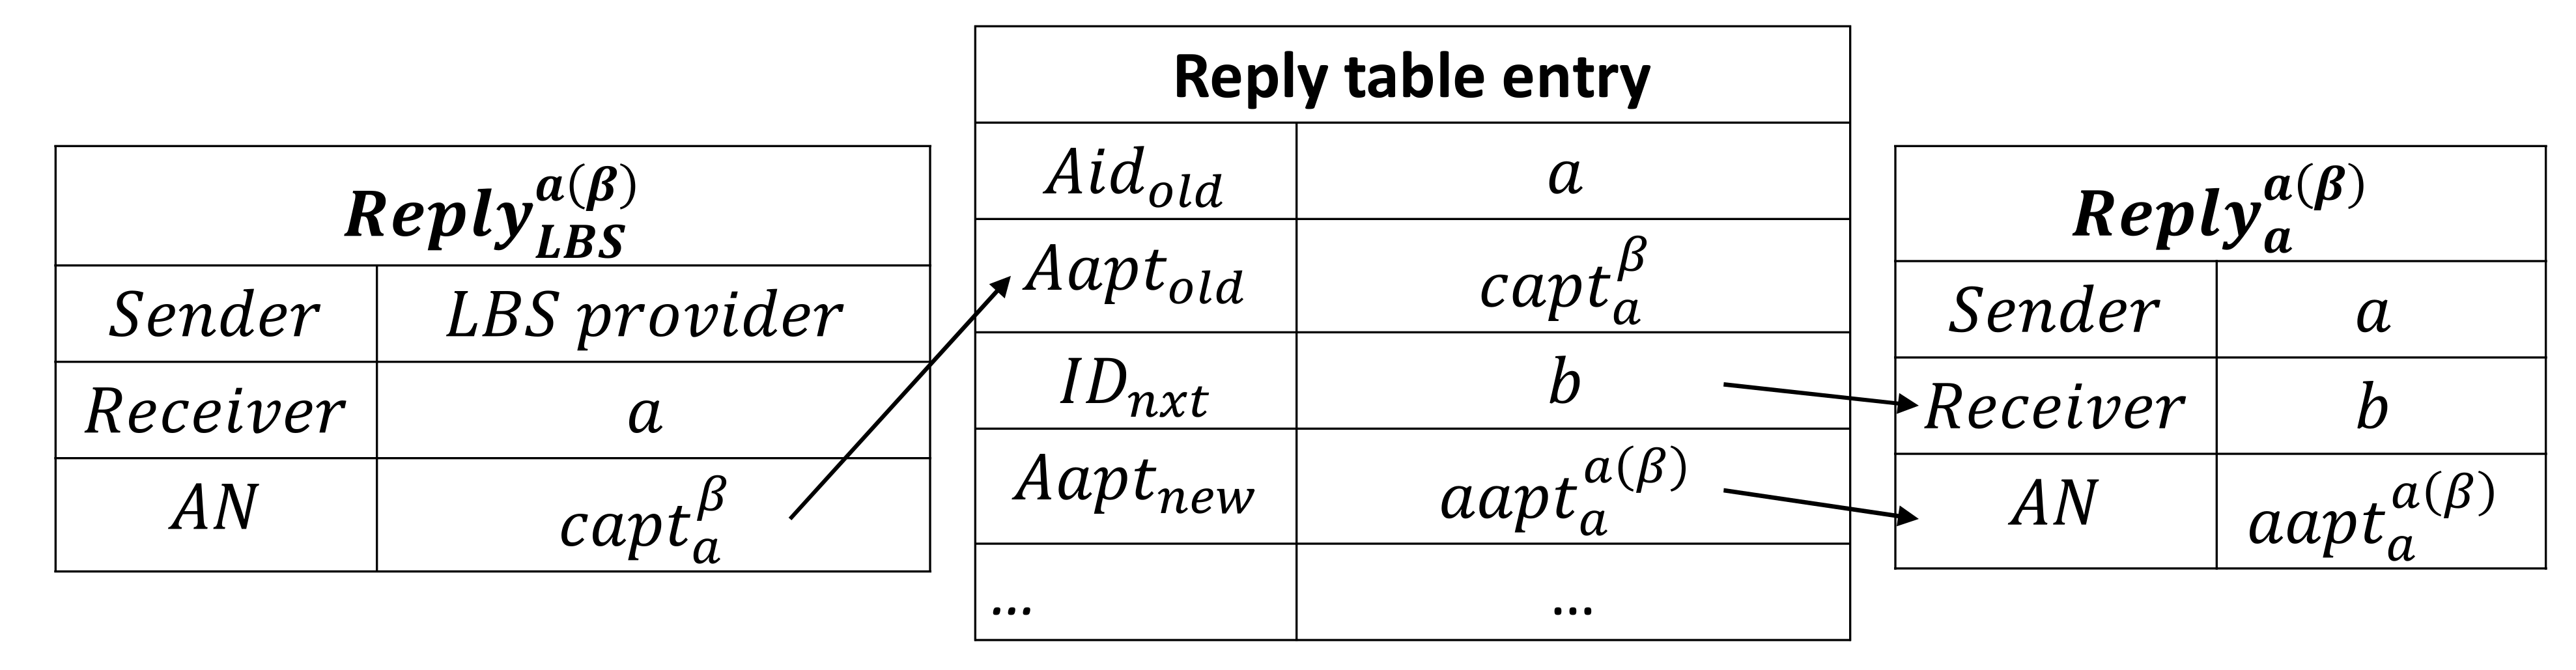
\includegraphics[width=6.0in]{figures/FIG_4_7_The_Reply_of_The_First_Agent.png}
\caption{The Reply of The First Agent} 
\label{fig:ReplyOfFirstAgent} %% label for entire figure 
\end{figure}

\subsubsection{Intermediate Agents}

\noindent The process of forwarding replies in the intermediate agents (the second to the ${\left(k-1\right)}^{th}$ one) is similar to that of the first agent. We take the second agent as an example. When the second agent receives the reply forwarded by the first one, he learns the sender's identity (i.e., the first agent) and the $AN$ from the reply. In his \textit{reply-table} shown in Table \ref{table:RTESecondAgt}, there must be an entry which is related to the AC which is used in the reply (query), because he gets the AC from the previous agent. More specifically, his \textit{reply-table} must include an entry whose ${Aid}_{old}$ is equal to the previous agent's identity and the ${Aapt}_{old}$ is the value of $AN$ in the received reply.

\begin{table} [hbtp]
\caption{Reply Table Entries of The Second Agent}
\label{table:RTESecondAgt}
\centering
\tabulinesep=2mm
\begin{tabu} to 135 mm {|X[1,c]|X[3,l]|} \hline 
%\begin{tabular}{|c|l|} \hline 
Name of Entries & Value \\ \hline 
${Aid}_{old}$ & The identity of the previous agent (i.e. the first agent) \\ \hline 
${Aapt}_{old}$ & The $Aapt$ given by the previous agent. \\ \hline 
${ID}_{nxt}$ & The identity of the next agent (e.g. the third agent) \\ \hline 
${Aapt}_{new}$ & The $Aapt$ given to the next agent by the user. \\ \hline 
\textit{EQL} & 2 \\ \hline 
$AT$ & The time when the AC times out. \\ \hline 
\end{tabu}
%\end{tabular}
\end{table}

For the example in Figure \ref{fig:EoACPME}, the second agent is $U_b$. When he receives ${Reply}^{a\left(\beta\right)}_a$, he learns that it is $U_a$ who forwards the reply message ${Reply}^{a\left(\beta\right)}_a$ and the $Aapt$ of the AC is ${aapt}^{a\left(\beta\right)}_a$. He searches his \textit{reply-table} for an entry whose ${Aid}_{old}$ is equal to $a$ and ${Aapt}_{old}$ is equal to ${aapt}^{a\left(\beta\right)}_a$. As shown in Figure \ref{fig:ReplyOfSecondAgent}, since the ${ID}_{nxt}$ in the entry is equal to $c$, he modifies the receiver of the reply message to $U_c$. $U_b$ also modifies the $AN$ in the reply message to ${aapt}^{a\left(\beta\right)}_b$ which enables $U_c$ identifies the AC in his \textit{reply-table}, because the ${Aapt}_{new}$ in the entry is equal to ${aapt}^{a\left(\beta\right)}_b$. 

\begin{figure} [H]
\centering 
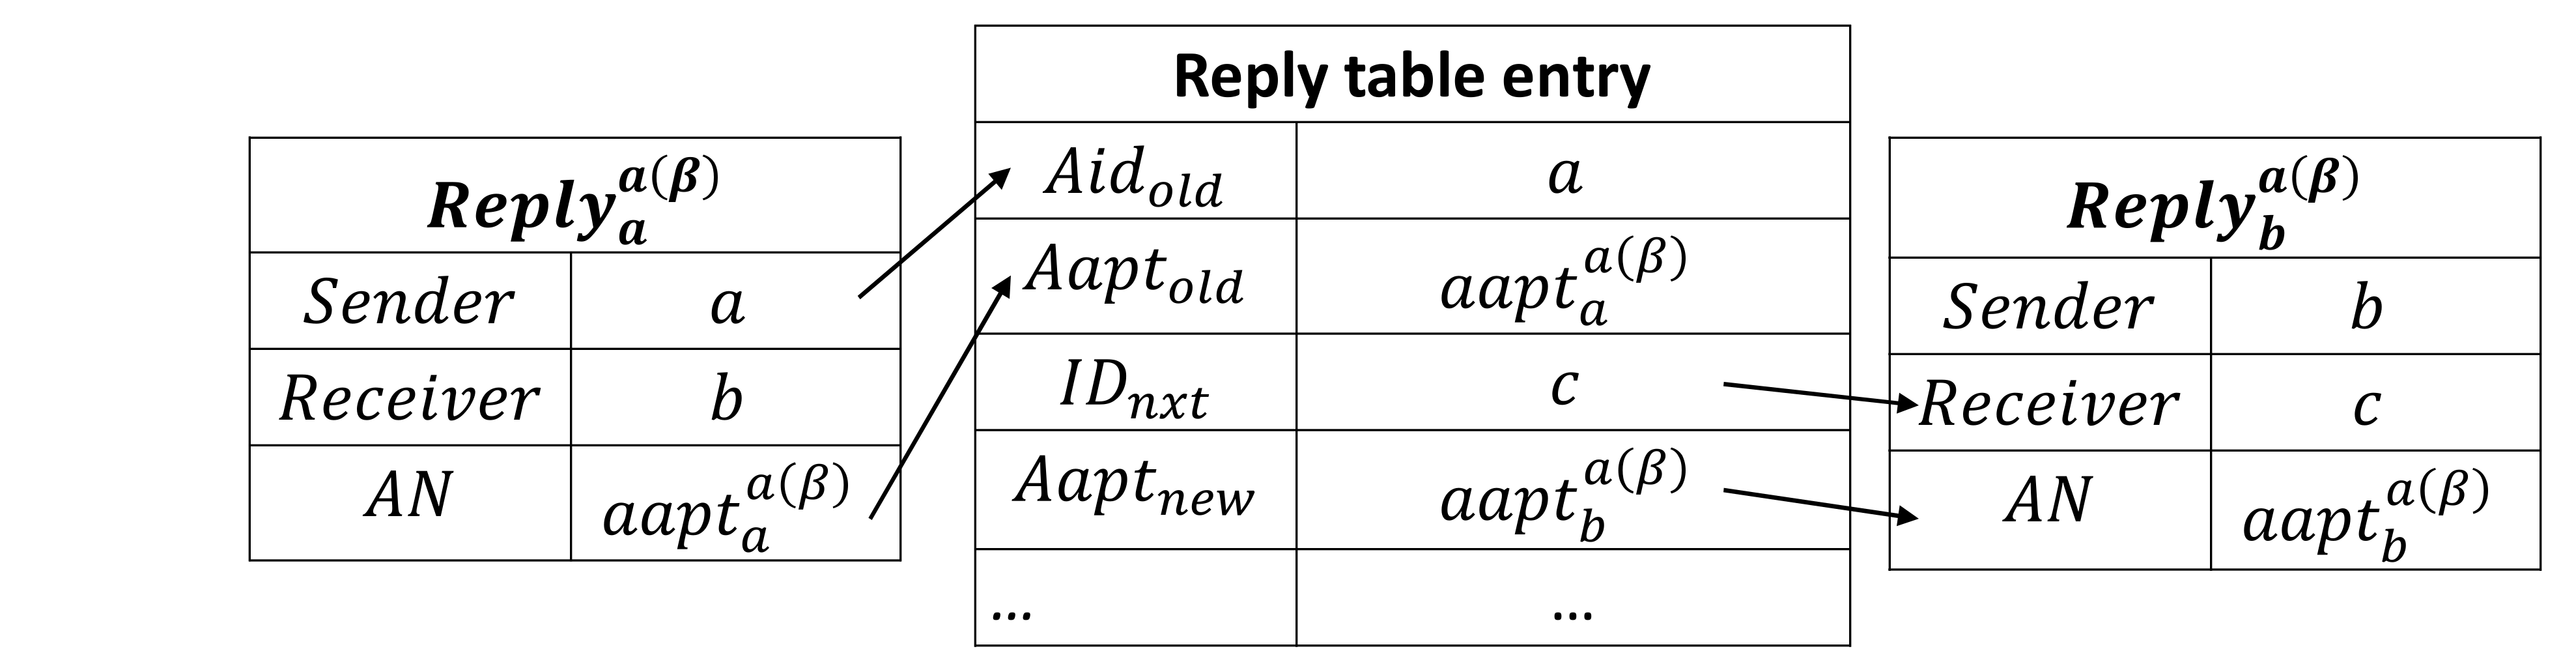
\includegraphics[width=6.0in]{figures/FIG_4_8_The_Reply_of_the_Second_Agent.png}
\caption{The Reply of The Second Agent} 
\label{fig:ReplyOfSecondAgent} %% label for entire figure 
\end{figure}

For each agent ${Agt}_i$, where $2\le i\le k-1$, he searches his \textit{reply-table} for the corresponding entry when he receives a reply. The ${Aid}_{old}$ and ${Aapt}_{old}$ in the entry should be equal to the sender's identity and the $AN$ in the reply. The identity of the next agent ${Agt}_{i+1}$ is ${ID}_{nxt}$. ${Agt}_i$ also assigns ${Aapt}_{new}$ to the $AN$ in the reply to help ${Agt}_{i+1}$ search ${Agt}_{i+1}$'s \textit{reply-table}.

\subsubsection{The Last Agent} \label{paraLastAgent}

\noindent The last agent also searches for a \textit{reply-table} entry based on the reply, while he cannot get the identity of the next agent. The \textit{reply-table} entry of the last agent is shown in Table \ref{table:RTELastAgt}.

\begin{table} [hbtp]
\caption{Reply Table Entries of The Last Agent}
\label{table:RTELastAgt}
\centering
\tabulinesep=2mm
\begin{tabu} to 135 mm {|X[1,c]|X[3,l]|} \hline 
%\begin{tabular}{|c|l|} \hline 
Name of Entries & Value \\ \hline 
${Aid}_{old}$ & The identity of the previous agent (i.e., the second agent) \\ \hline 
${Aapt}_{old}$ & The $Aapt$ given by the previous agent. \\ \hline 
${ID}_{nxt}$ & VOID \\ \hline 
${Aapt}_{new}$ & The $Aapt$ given to the original requester. \\ \hline 
\textit{EQL} & $k$ \\ \hline 
$AT$ & The time when the AC times out. \\ \hline 
\end{tabu}
%\end{tabular}
\end{table}

The last agent uses the same way to look up the entry in his \textit{reply-table} based on the reply. When he finds that the \textit{EQL} is equal to $k$, he notices that he is the last agent. Then, he is responsible for forwarding the reply to the original requester instead of forwarding to another agent. He uses his identity and ${Aapt}_{new}$ in his \textit{reply-table} entry to generates a pseudonym as follows:

\begin{equation} \label{GrindEQ__ACPPsd} 
{psd}_{{Agt}_k}^{a\left( \beta \right)}=pseudo\left({Agt}_k,{Aapt}_{new}\right)
\end{equation}

where the function $pseudo\left(id,Aapt\right)$ is a public pseudonym generating function which everyone in the network knows, including the original requester.

When the original requester sends his query, he also gets the same pseudonym ${psd}_{{Agt}_k}^{a\left( \beta \right)}$ using the pseudonym generating function. Note that he can get parameters from the AC. ${Agt}_k$ and ${Aapt}_{new}$ are equal to the $Aid$ and $Aapt$ in the AC. He uses that pseudonym as his identity before he gets the reply.

When users deliver the reply from the last agent, they are looking for an user whose identity is that pseudonym. At last, the original requester gets the reply, because he is the only user who uses the pseudonym as his identity.

For the example in Figure \ref{fig:EoACPME}, the last agent is $U_c$. When he receives ${Reply}^{a\left(\beta\right)}_b$, he learns that it is $U_b$ who forwards the reply message ${Reply}^{a\left(\beta\right)}_b$ and the $Aapt$ of the AC is ${aapt}^{a\left(\beta\right)}_b$. He searches his \textit{reply-table} for an entry whose ${Aid}_{old}$ is equal to $b$ and ${Aapt}_{old}$ is equal to ${aapt}^{a\left(\beta\right)}_b$. Since the \textit{EQL} in the entry is equal to 3 (i.e. $k$), he recognizes that he is the last agent. $U_c$ calculates the pseudonym ${psd}^{a\left(\beta \right)}_c=pseudo\left(c,{aapt}^{a\left(\beta\right)}_c\right)$ then forward the reply to ${psd}^{a\left(\beta\right)}_c$. The original requester $d$ gets the identity $c$ and the ${aapt}^{a\left(\beta \right)}_c$ from the AC he uses, so that he uses the pseudonym ${psd}^{a\left(\beta \right)}_c$ as his identity. As a result, $U_d$ get the reply from $U_c$. The $AN$ of the reply is also assigned to ${aapt}^{a\left(\beta\right)}_c$ to avoid identical pseudonyms. The process is shown in Figure \ref{fig:ReplyOfLastAgent}. 

\begin{figure} [hbtp]
\centering 
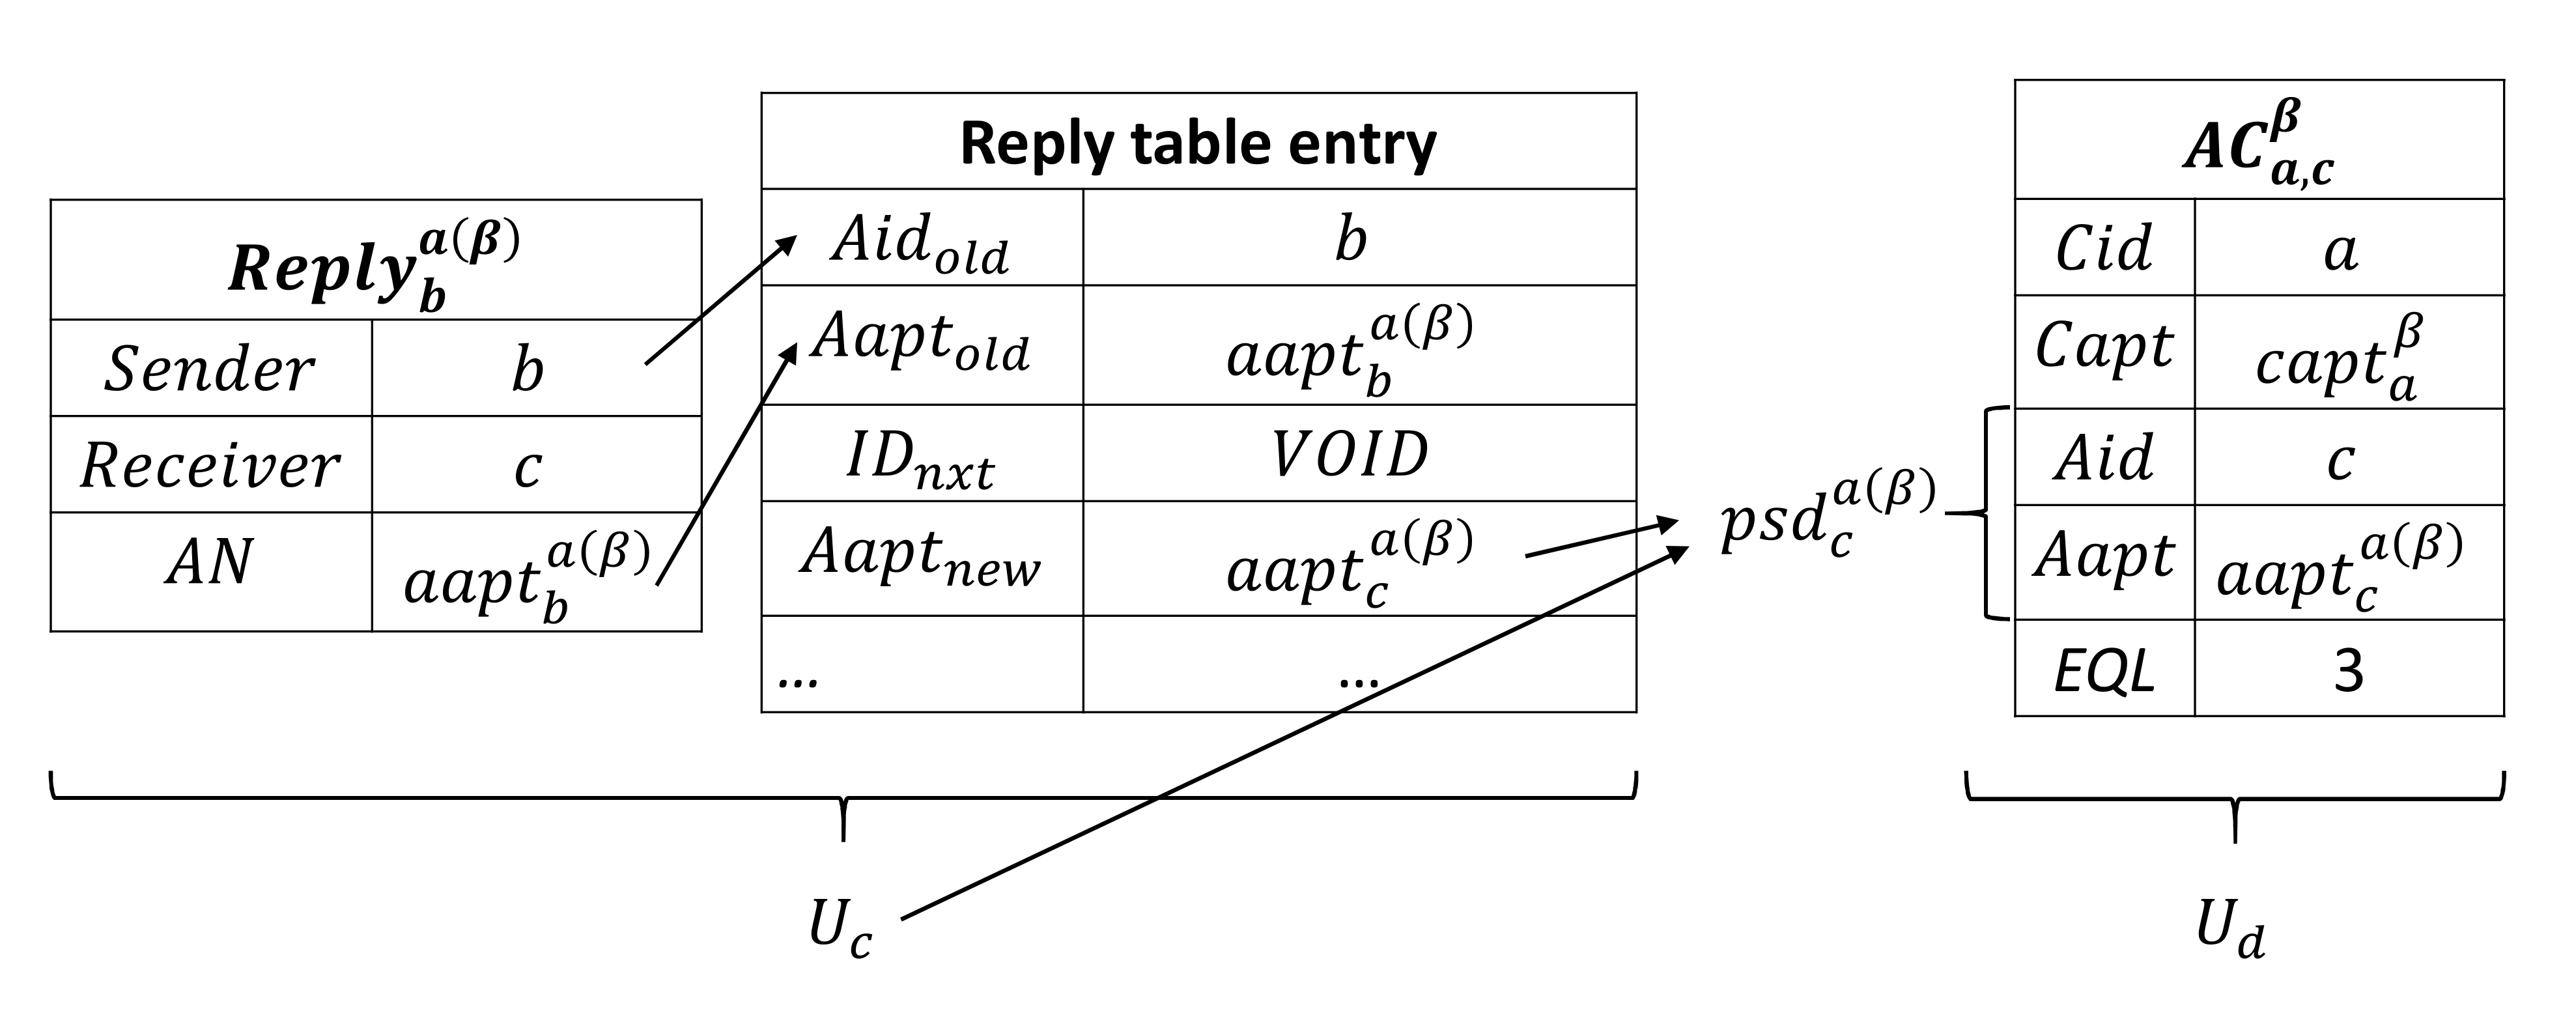
\includegraphics[width=6.0in]{figures/FIG_4_9_The_Reply_of_the_Last_Agent.png}
\caption{The Reply of the Last Agent} 
\label{fig:ReplyOfLastAgent} %% label for entire figure 
\end{figure}

The algorithm of forwarding replies when an agent $U_i$ gets a reply message from $U_{prev}$ is shown in Algorithm \ref{AlgACPForwardReply}. $U_i$ learns the $AN$ and the identity of the sender from the reply message ${Reply}_{U_{prev}}^{\alpha\left(\beta\right)}$. Based on this information, $U_i$ checks his \textit{reply-table} to find out where the reply should be forwarded to, which is ${ID}_{nxt}$. After $U_i$ updates the $AN$ of the reply message, he forwards the reply message to ${ID}_{nxt}$.

\begin{algorithm} [hbtp]
\caption{Algorithm For Forwarding Replies}\label{AlgACPForwardReply}
\begin{algorithmic}[1]
\Procedure {Received} {${Reply}_{U_{prev}}^{\alpha\left(\beta\right)}$}
\State Get the $AN$ from ${Reply}_{U_{prev}}^{\alpha\left(\beta\right)}$
\If {$U_{prev}$ is the LBS}
\State search $U_i$’s \textit{relay-table} to find an entry $E_i^{\alpha\left(\beta\right)}$
\State whose ${Aapt}_{old}=AN$ and ${Aid}_{old}=U_i$
\Else
\State search $U_i$’s \textit{relay-table} to find an entry $E_i^{\alpha\left(\beta\right)}$
\State whose ${Aapt}_{old}=AN$ and ${Aid}_{old}=U_{prev}$ 
\EndIf
\State Get the \textit{EQL}, ${Aapt}_{new}$ and ${ID}_{nxt}$ from $E_i^{\alpha\left(\beta\right)}$
\State Assign the $AN$ of ${Reply}_{U_{prev}}^{\alpha\left(\beta\right)}$ to ${Aapt}_{new}$.
\State Assign the sender identity to $U_i$.
\If {$EQL=k$}
\State ${ID}_{nxt}\gets pseudo\left(U_i,{Aapt}_{new}\right)$
\EndIf
\State Forward the reply to ${ID}_{nxt}$
\EndProcedure

\end{algorithmic}
\end{algorithm}

\section{Appointment Number}

\noindent The Appointment Number ($AN$) including $Capt$ and $Aapt$ is significant information in the AC. We explain the rules of generating them in detail and talk about the effect of ACs' timeout mechanism in this section.


\subsection{Creator Appointment Number}

\noindent The Creator Appointment Number ($Capt$) is a number which is used to identify ACs generated by the same creator. In other words, if two ACs are generated by the same creator, and they do not expire, their $Capt$ must be different. Therefore, the first agent (i.e., the creator) cannot find two entries which have the same ${Aapt}_{old}$ in his \textit{reply-table}, if their ${Aid}_{old}$ are both his own identity.


\subsection{Agent Appointment Number}

\noindent The Agent appointment number ($Aapt$) is a number used to identify appointment cards which have the same agent. Agents generate a new $Aapt$s for appointment cards before they exchange those cards to others. In other words, an agent gives any appointment card passing on by him a unique $Aapt$, which helps the next agent identify the appointment card in his \textit{reply-table}. Since the $Aapt$ is unique, an agent who is not the first one cannot find the replicated pair, ${Aid}_{old}$ and ${Aapt}_{old}$, in his \textit{reply-table}.


\subsection{Timeout}

\noindent Agents delete the entries, which contains the information of expired ACs, from his \textit{reply-table}. Consequently, agents cannot forward replies using ACs which expire. That is the reason why an original requester must choose an AC which expires after his query and reply timeout. However, the timeout mechanism is still necessary for the protocol.

Since users are moving, the distance between agents and the original requester might be too large after a long time. As a result, it is hard for agents to forward the reply messages back to the original requester so that the original requester takes a higher risk when he uses an AC which exists for a long time. Then this kind of ACs might not be used after a period, while it cost agents a few memories to save the ACs' information in their \textit{reply-table}. Therefore, all users remove the information of expired ACs to save their memories.

We should also notice that an unexpired AC and an expired one might have the same $Capt$ or $Aapt$. Because no agent keeps the record of the expired AC, the duplication cannot confuse agents.







\section{ Example}

\noindent In the following example, we use 5 users (i.e., Alice, Bob, Charlie, David and Elizabeth) to show the process of ACP. We should notice that David trusts Charlie (Charlie does not trust David), Elizabeth trusts David (David does not trust Elizabeth). Users do not trust others except the above two pairs. The parameters are shown in Table \ref{table:ACPExampleParameters}.

\begin{table} [hbtp]
\caption{Example Parameters}
\label{table:ACPExampleParameters}
\centering
\tabulinesep=2mm
\begin{tabu}{|c|c|} \hline 
%\begin{tabular}{|c|l|} \hline 
Parameters & Explanation \\ \hline 
${k}$ & 3 \\ \hline 
${m}$ & 1 \\ \hline 
${Seg}$ & 2 \\ \hline 
${GP}$ & 10 minutes \\ \hline 
${AT}$ & 80 minutes \\ \hline 
${\tau}$ & 80 minutes (equal to ${AT}$) \\ \hline 
%\end{tabular}
\end{tabu}
\end{table}

We abstract the event that users encounter each other in Table \ref{table:ACPExampleEvent}. Let $t_i$ denote the $i^{th}$ minute. The table lists the time when two users encounter each other. For example, Charlie and Elizabeth encounter each other at the third minute ($t_3$). After two users meet, they separate in one minute. 

\begin{table} [hbtp]
\caption{Example Event}
\label{table:ACPExampleEvent}
\centering
\tabulinesep=2mm
\begin{tabu}{|c|c|c|} \hline 
%\begin{tabular}{|c|l|} \hline 
User 1 & User 2 & Time \\ \hline 
Elizabeth & Bob & $t_1$ \\ \hline 
Bob & Charlie & $t_2$ \\ \hline 
Charlie & Elizabeth & $t_3$ \\ \hline 
Elizabeth & Alice & $t_4$ \\ \hline 
Bob & Charlie & $t_5$ \\ \hline 
Alice & Charlie & $t_6$ \\ \hline 
Charlie & David & $t_7$ \\ \hline 
David & Elizabeth & $t_8$ \\ \hline 
%\end{tabular}
\end{tabu}
\end{table}

We assume that these users do not encounter any user for a long time, so that they each has 8 ($=\frac{80min}{10min}$) ACs generated by themselves. We also assume that no AC expires in our 8-minutes example. Since the parameter \textit{Seg} is equal to 2, each user has 2 \textit{Distributing} AC Lists (\textit{DL}s). The initial state of our example is shown in Table \ref{table:ACPExampleInitialState}. To make the example simple and clear, we do not place ACs in \textit{DL}s randomly, ACs are always placed in the DL alternately. For example, if we put the first AC in \textit{DL}1, then the second AC must be in the \textit{DL}2. Users also obey the rule when they receive ACs from other users.

\begin{table} [hbtp]
\caption{Example Initial State}
\label{table:ACPExampleInitialState}
\centering
\tabulinesep=2mm
\begin{tabu}{|c|l|l|l|} \hline 
User Identity & \textit{DL}1 & \textit{DL}2 & \textit{RL} \\ \hline 
Alice (A) & ${\mathrm{AC}}^{\mathrm{1}\left[0\right]}_{\mathrm{A}},{\mathrm{AC}}^{\mathrm{3}\left[0\right]}_{\mathrm{A}},{\mathrm{AC}}^{\mathrm{5}\left[0\right]}_{\mathrm{A}},{\mathrm{AC}}^{\mathrm{7}\left[0\right]}_{\mathrm{A}}$ & ${\mathrm{AC}}^{\mathrm{2}\left[0\right]}_{\mathrm{A}},{\mathrm{AC}}^{\mathrm{4}\left[0\right]}_{\mathrm{A}},{\mathrm{AC}}^{\mathrm{6}\left[0\right]}_{\mathrm{A}},{\mathrm{AC}}^{\mathrm{8}\left[0\right]}_{\mathrm{A}}$ & $\mathrm{\emptyset }$ \\ \hline 
Bob (B) & ${\mathrm{AC}}^{\mathrm{1}\left[0\right]}_{\mathrm{B}},{\mathrm{AC}}^{\mathrm{3}\left[0\right]}_{\mathrm{B}},{\mathrm{AC}}^{\mathrm{5}\left[0\right]}_{\mathrm{B}},{\mathrm{AC}}^{\mathrm{7}\left[0\right]}_{\mathrm{B}}$ & ${\mathrm{AC}}^{\mathrm{2}\left[0\right]}_{\mathrm{B}},{\mathrm{AC}}^{\mathrm{4}\left[0\right]}_{\mathrm{B}},{\mathrm{AC}}^{\mathrm{6}\left[0\right]}_{\mathrm{B}},{\mathrm{AC}}^{\mathrm{8}\left[0\right]}_{\mathrm{B}}$ & $\mathrm{\emptyset }$ \\ \hline 
Charlie (C) & ${\mathrm{AC}}^{\mathrm{1}\left[0\right]}_{\mathrm{C}},{\mathrm{AC}}^{\mathrm{3}\left[0\right]}_{\mathrm{C}},{\mathrm{AC}}^{\mathrm{5}\left[0\right]}_{\mathrm{C}},{\mathrm{AC}}^{\mathrm{7}\left[0\right]}_{\mathrm{C}}$ & ${\mathrm{AC}}^{\mathrm{2}\left[0\right]}_{\mathrm{C}},{\mathrm{AC}}^{\mathrm{4}\left[0\right]}_{\mathrm{C}},{\mathrm{AC}}^{\mathrm{6}\left[0\right]}_{\mathrm{C}},{\mathrm{AC}}^{\mathrm{8}\left[0\right]}_{\mathrm{C}}$ & $\mathrm{\emptyset }$ \\ \hline 
David (D) & ${\mathrm{AC}}^{\mathrm{1}\left[0\right]}_{\mathrm{D}},{\mathrm{AC}}^{\mathrm{3}\left[0\right]}_{\mathrm{D}},{\mathrm{AC}}^{\mathrm{5}\left[0\right]}_{\mathrm{D}},{\mathrm{AC}}^{\mathrm{7}\left[0\right]}_{\mathrm{D}}$ & ${\mathrm{AC}}^{\mathrm{2}\left[0\right]}_{\mathrm{D}},{\mathrm{AC}}^{\mathrm{4}\left[0\right]}_{\mathrm{D}},{\mathrm{AC}}^{\mathrm{6}\left[0\right]}_{\mathrm{D}},{\mathrm{AC}}^{\mathrm{8}\left[0\right]}_{\mathrm{D}}$ & $\mathrm{\emptyset }$ \\ \hline 
Elizabeth (E) & ${\mathrm{AC}}^{\mathrm{1}\left[0\right]}_{\mathrm{E}},{\mathrm{AC}}^{\mathrm{3}\left[0\right]}_{\mathrm{E}},{\mathrm{AC}}^{\mathrm{5}\left[0\right]}_{\mathrm{E}},{\mathrm{AC}}^{\mathrm{7}\left[0\right]}_{\mathrm{E}}$ & ${\mathrm{AC}}^{\mathrm{2}\left[0\right]}_{\mathrm{E}},{\mathrm{AC}}^{\mathrm{4}\left[0\right]}_{\mathrm{E}},{\mathrm{AC}}^{\mathrm{6}\left[0\right]}_{\mathrm{E}},{\mathrm{AC}}^{\mathrm{8}\left[0\right]}_{\mathrm{E}}$ & $\mathrm{\emptyset }$ \\ \hline 
\end{tabu}
\end{table}

The explanation of symbols used in table are shown in the former Table \ref{table:ACPSymbols}. To make the symbol clear, we add the \textit{EQL} of the AC on the superscript. For example, if the \textit{EQL} of ${AC}^1_{A,X}$ is equal to 2, it is marked as ${AC}^{1\left[2\right]}_{A,X}$.


\subsection{ Exchanging Appointment Cards}

\noindent To make it easier, users do not pick \textit{DL}s randomly as we described in the previous sections when they exchange ACs. Instead, If we say that $U_x$ encounters $U_y$, $U_x$ always picks his \textit{DL}1 and $U_y$ always picks his \textit{DL}2. 

The tables in current section show the entire \textit{distributing}-AC Lists (i.e., \textit{DL}1 and \textit{DL}2) and entire \textit{relay-table}s (\textit{RL}s) of each user. We use the initial letter to denote each user in symbols. For example, D denotes David. The structure of the AC-list tables is shown in Table \ref{table:ACPXYACLists}.

\begin{table} [H]
\caption{User X and Y's AC Lists}
\label{table:ACPXYACLists}
\centering
\tabulinesep=2mm
\begin{tabu}{|c|c|c|l|} \hline 
\multirow{6}*{X} & \multirow{2}*{\textit{DL}1} & Before & X's \textit{distributing}-AC list 1 before their exchange. \\ \cline{3-4}
 &  & After & X's \textit{distributing}-AC list 1 after their exchange. \\ \cline{2-4} 
 & \multirow{2}*{\textit{DL}2} & Before & X's \textit{distributing}-AC list 2 before their exchange. \\ \cline{3-4} 
 &  & After & X's \textit{distributing}-AC list 2 after their exchange. \\ \cline{2-4} 
 &\multirow{2}*{ \textit{RL}} & Before & X's \textit{ready}-AC list before their exchange. \\ \cline{3-4} 
 &  & After & X's \textit{ready}-AC list after their exchange. \\ \hline 
\multirow{6}*{Y} & \multirow{2}*{\textit{DL}1} & Before & Y's \textit{distributing}-AC list 1 before their exchange. \\ \cline{3-4} 
 &  & After & Y's \textit{distributing}-AC list 1 after their exchange. \\ \cline{2-4} 
 & \multirow{2}*{\textit{DL}2} & Before & Y's \textit{distributing}-AC list 2 before their exchange. \\ \cline{3-4} 
 &  & After & Y's \textit{distributing}-AC list 2 after their exchange. \\ \cline{2-4} 
 & \multirow{2}*{\textit{RL}} & Before & Y's \textit{ready}-AC list before their exchange. \\ \cline{3-4} 
 &  & After & Y's \textit{ready}-AC list after their exchange. \\ \hline 
\end{tabu}
\end{table}

The process of exchanging AC is shown step by step as follows.

\noindent 1.  Elizabeth encounters Bob

At $t_1$ (the first minute), Elizabeth encounters Bob. Elizabeth picks her \textit{DL}1, and Bob picks his \textit{DL}2. They give \textit{distributing}-ACs in their picked \textit{DL}s to each other and update their reply tables, as shown in Table \ref{table:EBAcListT1} and Table \ref{table:EBReplyTableT1}.

\begin{table} [H]
\caption{Elizabeth and Bob's AC Lists at Time $t_1$}
\label{table:EBAcListT1}
\centering
\tabulinesep = 1mm
\begin{tabu}{|c|c|c|l|} \hline
\multirow{6}*{Elizabeth} & \multirow{2}*{\textit{DL}1} & Before & ${AC}_{E}^{1\left[0\right]}$,${AC}_{E}^{3\left[0\right]}$,${AC}_{E}^{5\left[0\right]}$,${AC}_{E}^{7\left[0\right]}$ \\ \cline{3-4}
 &  & After & ${AC}_{B,B}^{2\left[1\right]}$,${AC}_{B,B}^{6\left[1\right]}$ \\ \cline{2-4}
 & \multirow{2}*{\textit{DL}2} & Before & ${AC}_{E}^{2\left[0\right]}$,${AC}_{E}^{4\left[0\right]}$,${AC}_{E}^{6\left[0\right]}$,${AC}_{E}^{8\left[0\right]}$ \\ \cline{3-4}
 &  & After & ${AC}_{E}^{2\left[0\right]}$,${AC}_{E}^{4\left[0\right]}$,${AC}_{E}^{6\left[0\right]}$,${AC}_{E}^{8\left[0\right]}$,${AC}_{B,B}^{4\left[1\right]}$,${AC}_{B,B}^{8\left[1\right]}$ \\ \cline{2-4}
 & \multirow{2}*{\textit{RL}} & Before & $\emptyset$ \\ \cline{3-4}
 &  & After & $\emptyset$ \\ \hline
\multirow{6}*{Bob} & \multirow{2}*{\textit{DL}1} & Before & ${AC}_{B}^{1\left[0\right]}$,${AC}_{B}^{3\left[0\right]}$,${AC}_{B}^{5\left[0\right]}$,${AC}_{B}^{7\left[0\right]}$ \\ \cline{3-4}
 &  & After & ${AC}_{B}^{1\left[0\right]}$,${AC}_{B}^{3\left[0\right]}$,${AC}_{B}^{5\left[0\right]}$,${AC}_{B}^{7\left[0\right]}$,${AC}_{E,E}^{1\left[1\right]}$,${AC}_{E,E}^{5\left[1\right]}$ \\ \cline{2-4}
 & \multirow{2}*{\textit{DL}2} & Before & ${AC}_{B}^{2\left[0\right]}$,${AC}_{B}^{4\left[0\right]}$,${AC}_{B}^{6\left[0\right]}$,${AC}_{B}^{8\left[0\right]}$ \\ \cline{3-4}
 &  & After & ${AC}_{E,E}^{3\left[1\right]}$,${AC}_{E,E}^{7\left[1\right]}$ \\ \cline{2-4}
 & \multirow{2}*{\textit{RL}} & Before & $\emptyset$ \\ \cline{3-4}
 &  & After & $\emptyset$ \\ \hline
\end{tabu}
\end{table}

\begin{table} [H]
\caption{Elizabeth and Bob's Relay Table At Time $t_1$}
\label{table:EBReplyTableT1}
\centering
\tabulinesep = 1mm
\begin{tabu}{|c|c|c|c|c|c|c|c|c|c|} \hline
\multicolumn{5}{|c|}{Elizabeth} & \multicolumn{5}{|c|}{Bob} \\ \hline
${Aid}_{old}$ & ${Aapt}_{old}$ & ${ID}_{nxt}$ & ${Aapt}_{new}$ & \textit{EQL} & ${Aid}_{old}$ & ${Aapt}_{old}$ & ${ID}_{nxt}$ & ${Aapt}_{new}$ & \textit{EQL} \\ \hline
$E$ & ${capt}_{E}^{1}$ & $B$ & ${aapt}_{E}^{E\left(1\right)}$ & $1$ & $B$ & ${capt}_{B}^{2}$ & $E$ & ${aapt}_{B}^{B\left(2\right)}$ & $1$ \\ \hline
$E$ & ${capt}_{E}^{3}$ & $B$ & ${aapt}_{E}^{E\left(3\right)}$ & $1$ & $B$ & ${capt}_{B}^{4}$ & $E$ & ${aapt}_{B}^{B\left(4\right)}$ & $1$ \\ \hline
$E$ & ${capt}_{E}^{5}$ & $B$ & ${aapt}_{E}^{E\left(5\right)}$ & $1$ & $B$ & ${capt}_{B}^{6}$ & $E$ & ${aapt}_{B}^{B\left(6\right)}$ & $1$ \\ \hline
$E$ & ${capt}_{E}^{7}$ & $B$ & ${aapt}_{E}^{E\left(7\right)}$ & $1$ & $B$ & ${capt}_{B}^{8}$ & $E$ & ${aapt}_{B}^{B\left(8\right)}$ & $1$ \\ \hline
\end{tabu}
\end{table}

\noindent 2.  Bob encounters Charlie

At $t_2$ (the second minute), Bob encounters Charlie. Bob picks his \textit{DL}1, and Charlie picks his \textit{DL}2. They give \textit{distributing}-ACs in their picked \textit{DL}s to each other and update their reply tables, as shown in Table \ref{table:BCAcListT2} and Table \ref{table:BCReplyTableT2}.

\begin{table} [H]
\caption{Bob and Charlie's AC Lists at Time $t_2$}
\label{table:BCAcListT2}
\centering
\tabulinesep = 1mm
\begin{tabu}{|c|c|c|l|} \hline
\multirow{6}*{Bob} & \multirow{2}*{\textit{DL}1} & Before & ${AC}_{B}^{1\left[0\right]}$,${AC}_{B}^{3\left[0\right]}$,${AC}_{B}^{5\left[0\right]}$,${AC}_{B}^{7\left[0\right]}$,${AC}_{E,E}^{1\left[1\right]}$,${AC}_{E,E}^{5\left[1\right]}$ \\ \cline{3-4}
 &  & After & ${AC}_{C,C}^{2\left[1\right]}$,${AC}_{C,C}^{6\left[1\right]}$ \\ \cline{2-4}
 & \multirow{2}*{\textit{DL}2} & Before & ${AC}_{E,E}^{3\left[1\right]}$,${AC}_{E,E}^{7\left[1\right]}$ \\ \cline{3-4}
 &  & After & ${AC}_{E,E}^{3\left[1\right]}$,${AC}_{E,E}^{7\left[1\right]}$,${AC}_{C,C}^{4\left[1\right]}$,${AC}_{C,C}^{8\left[1\right]}$ \\ \cline{2-4}
 & \multirow{2}*{\textit{RL}} & Before & $\emptyset$ \\ \cline{3-4}
 &  & After & $\emptyset$ \\ \hline
\multirow{6}*{Charlie} & \multirow{2}*{\textit{DL}1} & Before & ${AC}_{C}^{1\left[0\right]}$,${AC}_{C}^{3\left[0\right]}$,${AC}_{C}^{5\left[0\right]}$,${AC}_{C}^{7\left[0\right]}$ \\ \cline{3-4}
 &  & After & ${AC}_{C}^{1\left[0\right]}$,${AC}_{C}^{3\left[0\right]}$,${AC}_{C}^{5\left[0\right]}$,${AC}_{C}^{7\left[0\right]}$,${AC}_{B,B}^{1\left[1\right]}$,${AC}_{B,B}^{5\left[1\right]}$,${AC}_{E,B}^{1\left[2\right]}$ \\ \cline{2-4}
 & \multirow{2}*{\textit{DL}2} & Before & ${AC}_{C}^{2\left[0\right]}$,${AC}_{C}^{4\left[0\right]}$,${AC}_{C}^{6\left[0\right]}$,${AC}_{C}^{8\left[0\right]}$ \\ \cline{3-4}
 &  & After & ${AC}_{B,B}^{3\left[1\right]}$,${AC}_{B,B}^{7\left[1\right]}$,${AC}_{E,B}^{5\left[2\right]}$ \\ \cline{2-4}
 & \multirow{2}*{\textit{RL}} & Before & $\emptyset$ \\ \cline{3-4}
 &  & After & $\emptyset$ \\ \hline
\end{tabu}
\end{table}


\begin{table} [H]
\caption{Bob and Charlie's Relay Table At Time $t_2$}
\label{table:BCReplyTableT2}
\centering
\tabulinesep = 1mm
\begin{tabu}{|c|c|c|c|c|c|c|c|c|c|} \hline
\multicolumn{5}{|c|}{Bob} & \multicolumn{5}{|c|}{Charlie} \\ \hline
${Aid}_{old}$ & ${Aapt}_{old}$ & ${ID}_{nxt}$ & ${Aapt}_{new}$ & \textit{EQL} & ${Aid}_{old}$ & ${Aapt}_{old}$ & ${ID}_{nxt}$ & ${Aapt}_{new}$ & \textit{EQL} \\ \hline
$B$ & ${capt}_{B}^{2}$ & $E$ & ${aapt}_{B}^{B\left(2\right)}$ & $1$ & $C$ & ${capt}_{C}^{2}$ & $B$ & ${aapt}_{C}^{C\left(2\right)}$ & $1$ \\ \hline
$B$ & ${capt}_{B}^{4}$ & $E$ & ${aapt}_{B}^{B\left(4\right)}$ & $1$ & $C$ & ${capt}_{C}^{4}$ & $B$ & ${aapt}_{C}^{C\left(4\right)}$ & $1$ \\ \hline
$B$ & ${capt}_{B}^{6}$ & $E$ & ${aapt}_{B}^{B\left(6\right)}$ & $1$ & $C$ & ${capt}_{C}^{6}$ & $B$ & ${aapt}_{C}^{C\left(6\right)}$ & $1$ \\ \hline
$B$ & ${capt}_{B}^{8}$ & $E$ & ${aapt}_{B}^{B\left(8\right)}$ & $1$ & $C$ & ${capt}_{C}^{8}$ & $B$ & ${aapt}_{C}^{C\left(8\right)}$ & $1$ \\ \hline
$B$ & ${capt}_{B}^{1}$ & $C$ & ${aapt}_{B}^{B\left(1\right)}$ & $1$ &  &  &  &  &  \\ \hline
$B$ & ${capt}_{B}^{3}$ & $C$ & ${aapt}_{B}^{B\left(3\right)}$ & $1$ &  &  &  &  &  \\ \hline
$B$ & ${capt}_{B}^{5}$ & $C$ & ${aapt}_{B}^{B\left(5\right)}$ & $1$ &  &  &  &  &  \\ \hline
$B$ & ${capt}_{B}^{7}$ & $C$ & ${aapt}_{B}^{B\left(7\right)}$ & $1$ &  &  &  &  &  \\ \hline
$E$ & ${aapt}_{E}^{E\left(1\right)}$ & $C$ & ${aapt}_{B}^{E\left(1\right)}$ & $2$ &  &  &  &  &  \\ \hline
$E$ & ${aapt}_{E}^{E\left(5\right)}$ & $C$ & ${aapt}_{B}^{E\left(5\right)}$ & $2$ &  &  &  &  &  \\ \hline
\end{tabu}
\end{table}

\noindent 3.  Charlie encounters Elizabeth

At time ${t}_{3}$, Charlie encounters Elizabeth. Charlie picks his \textit{DL}1, and Elizabeth picks her \textit{DL}2. They give \textit{distributing}-ACs in their picked \textit{DL}s to each other and update their reply tables, as shown in Table \ref{table:CEAcListT3} and Table \ref{table:CEReplyTableT3}.

We should notice that Charlie does not give ${AC}^{1\left[2\right]}_{E,B}$ to Elizabeth, because Elizabeth does not trust Charlie. The \textit{EQL} of the ${AC}^{1\left[2\right]}_{E,B}$ has already reached 2, which is equal to $k-m=3-1$. As mentioned in subsection \ref{subsec_ExchangeDisAptCrd}, these kinds of ACs are only sent to users who trust the current agent. Therefore, Charlie cannot give ${AC}^{1\left[2\right]}_{E,B}$ to Elizabeth when she does not trust him.

\begin{table} [H]
\caption{Charlie and Elizabeth's AC Lists at Time $t_3$}
\label{table:CEAcListT3}
\centering
\tabulinesep = 1mm
\begin{tabu}{|c|c|c|l|} \hline
\multirow{6}*{Charlie} & \multirow{2}*{\textit{DL}1} & Before & ${AC}_{C}^{1\left[0\right]}$,${AC}_{C}^{3\left[0\right]}$,${AC}_{C}^{5\left[0\right]}$,${AC}_{C}^{7\left[0\right]}$,${AC}_{B,B}^{1\left[1\right]}$,${AC}_{B,B}^{5\left[1\right]}$,${AC}_{E,B}^{1\left[2\right]}$ \\ \cline{3-4}
 &  & After & ${AC}_{E,B}^{1\left[2\right]}$,${AC}_{E,E}^{2\left[1\right]}$,${AC}_{E,E}^{6\left[1\right]}$,${AC}_{B,E}^{4\left[2\right]}$ \\ \cline{2-4}
 & \multirow{2}*{\textit{DL}2} & Before & ${AC}_{B,B}^{3\left[1\right]}$,${AC}_{B,B}^{7\left[1\right]}$,${AC}_{E,B}^{5\left[2\right]}$ \\ \cline{3-4}
 &  & After & ${AC}_{B,B}^{3\left[1\right]}$,${AC}_{B,B}^{7\left[1\right]}$,${AC}_{E,B}^{5\left[2\right]}$,${AC}_{E,E}^{4\left[1\right]}$,${AC}_{E,E}^{8\left[1\right]}$,${AC}_{B,E}^{8\left[2\right]}$ \\ \cline{2-4}
 & \multirow{2}*{\textit{RL}} & Before & $\emptyset$ \\ \cline{3-4}
 &  & After & $\emptyset$ \\ \hline
\multirow{6}*{Elizabeth} & \multirow{2}*{\textit{DL}1} & Before & ${AC}_{B,B}^{2\left[1\right]}$,${AC}_{B,B}^{6\left[1\right]}$ \\ \cline{3-4}
 &  & After & ${AC}_{B,B}^{2\left[1\right]}$,${AC}_{B,B}^{6\left[1\right]}$,${AC}_{C,C}^{1\left[1\right]}$,${AC}_{C,C}^{5\left[1\right]}$,${AC}_{B,C}^{1\left[2\right]}$ \\ \cline{2-4}
 & \multirow{2}*{\textit{DL}2} & Before & ${AC}_{E}^{2\left[0\right]}$,${AC}_{E}^{4\left[0\right]}$,${AC}_{E}^{6\left[0\right]}$,${AC}_{E}^{8\left[0\right]}$,${AC}_{B,B}^{4\left[1\right]}$,${AC}_{B,B}^{8\left[1\right]}$ \\ \cline{3-4}
 &  & After & ${AC}_{C,C}^{3\left[1\right]}$,${AC}_{C,C}^{7\left[1\right]}$,${AC}_{B,C}^{5\left[2\right]}$ \\ \cline{2-4}
 & \multirow{2}*{\textit{RL}} & Before & $\emptyset$ \\ \cline{3-4}
 &  & After & $\emptyset$ \\ \hline
\end{tabu}
\end{table}

\begin{table} [H]
\caption{Charlie and Elizabeth's Relay Table At Time $t_3$}
\label{table:CEReplyTableT3}
\centering
\tabulinesep = 1mm
\begin{tabu}{|c|c|c|c|c|c|c|c|c|c|} \hline
\multicolumn{5}{|c|}{Charlie} & \multicolumn{5}{|c|}{Elizabeth} \\ \hline
${Aid}_{old}$ & ${Aapt}_{old}$ & ${ID}_{nxt}$ & ${Aapt}_{new}$ & \textit{EQL} & ${Aid}_{old}$ & ${Aapt}_{old}$ & ${ID}_{nxt}$ & ${Aapt}_{new}$ & \textit{EQL} \\ \hline
$C$ & ${capt}_{C}^{2}$ & $B$ & ${aapt}_{C}^{C\left(2\right)}$ & $1$ & $E$ & ${capt}_{E}^{1}$ & $B$ & ${aapt}_{E}^{E\left(1\right)}$ & $1$ \\ \hline
$C$ & ${capt}_{C}^{4}$ & $B$ & ${aapt}_{C}^{C\left(4\right)}$ & $1$ & $E$ & ${capt}_{E}^{3}$ & $B$ & ${aapt}_{E}^{E\left(3\right)}$ & $1$ \\ \hline
$C$ & ${capt}_{C}^{6}$ & $B$ & ${aapt}_{C}^{C\left(6\right)}$ & $1$ & $E$ & ${capt}_{E}^{5}$ & $B$ & ${aapt}_{E}^{E\left(5\right)}$ & $1$ \\ \hline
$C$ & ${capt}_{C}^{8}$ & $B$ & ${aapt}_{C}^{C\left(8\right)}$ & $1$ & $E$ & ${capt}_{E}^{7}$ & $B$ & ${aapt}_{E}^{E\left(7\right)}$ & $1$ \\ \hline
$C$ & ${capt}_{C}^{1}$ & $E$ & ${aapt}_{C}^{C\left(1\right)}$ & $1$ & $E$ & ${capt}_{E}^{2}$ & $C$ & ${aapt}_{E}^{E\left(2\right)}$ & $1$ \\ \hline
$C$ & ${capt}_{C}^{3}$ & $E$ & ${aapt}_{C}^{C\left(3\right)}$ & $1$ & $E$ & ${capt}_{E}^{4}$ & $C$ & ${aapt}_{E}^{E\left(4\right)}$ & $1$ \\ \hline
$C$ & ${capt}_{C}^{5}$ & $E$ & ${aapt}_{C}^{C\left(5\right)}$ & $1$ & $E$ & ${capt}_{E}^{6}$ & $C$ & ${aapt}_{E}^{E\left(6\right)}$ & $1$ \\ \hline
$C$ & ${capt}_{C}^{7}$ & $E$ & ${aapt}_{C}^{C\left(7\right)}$ & $1$ & $E$ & ${capt}_{E}^{8}$ & $C$ & ${aapt}_{E}^{E\left(8\right)}$ & $1$ \\ \hline
$B$ & ${aapt}_{B}^{B\left(1\right)}$ & $E$ & ${aapt}_{C}^{B\left(1\right)}$ & $2$ & $B$ & ${aapt}_{B}^{B\left(4\right)}$ & $C$ & ${aapt}_{E}^{B\left(4\right)}$ & $2$ \\ \hline
$B$ & ${aapt}_{B}^{B\left(5\right)}$ & $E$ & ${aapt}_{C}^{B\left(5\right)}$ & $2$ & $B$ & ${aapt}_{B}^{B\left(8\right)}$ & $C$ & ${aapt}_{E}^{B\left(8\right)}$ & $2$ \\ \hline
\end{tabu}
\end{table}

\noindent 4.  Elizabeth encounters Alice

At time $t_4$, Elizabeth encounters Alice. Elizabeth picks her \textit{DL}1, and Alice picks her \textit{DL}2. They give \textit{distributing}-ACs in their picked \textit{DL}s to each other and update their reply tables, as shown in Table \ref{table:EAAcListT4} and Table \ref{table:EAReplyTableT4}.

Elizabeth does not give ${AC}^{1\left[2\right]}_{B,C}$ to Alice for the same reason as the previous Charlie, that is, Alice does not trust Elizabeth.

\begin{table} [H]
\caption{Elizabeth and Alice's AC Lists at Time $t_4$}
\label{table:EAAcListT4}
\centering
\tabulinesep = 1mm
\begin{tabu}{|c|c|c|l|} \hline
\multirow{6}*{Elizabeth} & \multirow{2}*{\textit{DL}1} & Before & ${AC}_{B,B}^{2\left[1\right]}$,${AC}_{B,B}^{6\left[1\right]}$,${AC}_{C,C}^{1\left[1\right]}$,${AC}_{C,C}^{5\left[1\right]}$,${AC}_{B,C}^{1\left[2\right]}$ \\ \cline{3-4}
 &  & After & ${AC}_{B,C}^{1\left[2\right]}$,${AC}_{A,A}^{2\left[1\right]}$,${AC}_{A,A}^{6\left[1\right]}$ \\ \cline{2-4}
 & \multirow{2}*{\textit{DL}2} & Before & ${AC}_{C,C}^{3\left[1\right]}$,${AC}_{C,C}^{7\left[1\right]}$,${AC}_{B,C}^{5\left[2\right]}$ \\ \cline{3-4}
 &  & After & ${AC}_{C,C}^{3\left[1\right]}$,${AC}_{C,C}^{7\left[1\right]}$,${AC}_{B,C}^{5\left[2\right]}$,${AC}_{A,A}^{4\left[1\right]}$,${AC}_{A,A}^{8\left[1\right]}$ \\ \cline{2-4}
 & \multirow{2}*{\textit{RL}} & Before & $\emptyset$ \\ \cline{3-4}
 &  & After & $\emptyset$ \\ \hline
\multirow{6}*{Alice} & \multirow{2}*{\textit{DL}1} & Before & ${AC}_{A}^{1\left[0\right]}$,${AC}_{A}^{3\left[0\right]}$,${AC}_{A}^{5\left[0\right]}$,${AC}_{A}^{7\left[0\right]}$ \\ \cline{3-4}
 &  & After & ${AC}_{A}^{1\left[0\right]}$,${AC}_{A}^{3\left[0\right]}$,${AC}_{A}^{5\left[0\right]}$,${AC}_{A}^{7\left[0\right]}$,${AC}_{B,E}^{2\left[2\right]}$,${AC}_{C,E}^{1\left[2\right]}$ \\ \cline{2-4}
 & \multirow{2}*{\textit{DL}2} & Before & ${AC}_{A}^{2\left[0\right]}$,${AC}_{A}^{4\left[0\right]}$,${AC}_{A}^{6\left[0\right]}$,${AC}_{A}^{8\left[0\right]}$ \\ \cline{3-4}
 &  & After & ${AC}_{B,E}^{6\left[2\right]}$,${AC}_{C,E}^{5\left[2\right]}$ \\ \cline{2-4}
 & \multirow{2}*{\textit{RL}} & Before & $\emptyset$ \\ \cline{3-4}
 &  & After & $\emptyset$ \\ \hline
\end{tabu}
\end{table}

\begin{table} [H]
\caption{Elizabeth and Alice's Relay Table At Time $t_4$}
\label{table:EAReplyTableT4}
\centering
\tabulinesep = 1mm
\begin{tabu}{|c|c|c|c|c|c|c|c|c|c|} \hline
\multicolumn{5}{|c|}{Elizabeth} & \multicolumn{5}{|c|}{Alice} \\ \hline
${Aid}_{old}$ & ${Aapt}_{old}$ & ${ID}_{nxt}$ & ${Aapt}_{new}$ & \textit{EQL} & ${Aid}_{old}$ & ${Aapt}_{old}$ & ${ID}_{nxt}$ & ${Aapt}_{new}$ & \textit{EQL} \\ \hline
$E$ & ${capt}_{E}^{1}$ & $B$ & ${aapt}_{E}^{E\left(1\right)}$ & $1$ & $A$ & ${capt}_{A}^{2}$ & $E$ & ${aapt}_{A}^{A\left(2\right)}$ & $1$ \\ \hline
$E$ & ${capt}_{E}^{3}$ & $B$ & ${aapt}_{E}^{E\left(3\right)}$ & $1$ & $A$ & ${capt}_{A}^{4}$ & $E$ & ${aapt}_{A}^{A\left(4\right)}$ & $1$ \\ \hline
$E$ & ${capt}_{E}^{5}$ & $B$ & ${aapt}_{E}^{E\left(5\right)}$ & $1$ & $A$ & ${capt}_{A}^{6}$ & $E$ & ${aapt}_{A}^{A\left(6\right)}$ & $1$ \\ \hline
$E$ & ${capt}_{E}^{7}$ & $B$ & ${aapt}_{E}^{E\left(7\right)}$ & $1$ & $A$ & ${capt}_{A}^{8}$ & $E$ & ${aapt}_{A}^{A\left(8\right)}$ & $1$ \\ \hline
$E$ & ${capt}_{E}^{2}$ & $C$ & ${aapt}_{E}^{E\left(2\right)}$ & $1$ &  &  &  &  &  \\ \hline
$E$ & ${capt}_{E}^{4}$ & $C$ & ${aapt}_{E}^{E\left(4\right)}$ & $1$ &  &  &  &  &  \\ \hline
$E$ & ${capt}_{E}^{6}$ & $C$ & ${aapt}_{E}^{E\left(6\right)}$ & $1$ &  &  &  &  &  \\ \hline
$E$ & ${capt}_{E}^{8}$ & $C$ & ${aapt}_{E}^{E\left(8\right)}$ & $1$ &  &  &  &  &  \\ \hline
$B$ & ${aapt}_{B}^{B\left(4\right)}$ & $C$ & ${aapt}_{E}^{B\left(4\right)}$ & $2$ &  &  &  &  &  \\ \hline
$B$ & ${aapt}_{B}^{B\left(8\right)}$ & $C$ & ${aapt}_{E}^{B\left(8\right)}$ & $2$ &  &  &  &  &  \\ \hline
$B$ & ${aapt}_{B}^{B\left(2\right)}$ & $A$ & ${aapt}_{E}^{B\left(2\right)}$ & $2$ &  &  &  &  &  \\ \hline
$B$ & ${aapt}_{B}^{B\left(6\right)}$ & $A$ & ${aapt}_{E}^{B\left(6\right)}$ & $2$ &  &  &  &  &  \\ \hline
$C$ & ${aapt}_{C}^{C\left(1\right)}$ & $A$ & ${aapt}_{E}^{C\left(1\right)}$ & $2$ &  &  &  &  &  \\ \hline
$C$ & ${aapt}_{C}^{C\left(5\right)}$ & $A$ & ${aapt}_{E}^{C\left(5\right)}$ & $2$ &  &  &  &  &  \\ \hline
\end{tabu}
\end{table}

\noindent 5.  Bob encounters Charlie

At time ${t}_{5}$, Bob encounters Charlie. Bob picks his \textit{DL}1, and Charlie picks his \textit{DL}2. They give \textit{distributing}-ACs in their picked \textit{DL}s to each other and update their reply tables, as shown in Table \ref{table:BCAcListT5} and Table \ref{table:BCReplyTableT5}.

Charlie does not give ${AC}^{5\left[2\right]}_{E,B}$ and $\ {AC}^{8\left[2\right]}_{B,E}$ to Bob, because Bob does not trust Charlie. Since we set the avoiding time equal to \textit{AT}, a \textit{distributing}-AC cannot be given back to previous agents. As a result, ${AC}^{2\left[1\right]}_{C,C}$, ${AC}^{6\left[1\right]}_{C,C}$, ${AC}^{3\left[1\right]}_{B,B}$ and ${AC}^{7\left[1\right]}_{B,B}$ are not exchanged by Charlie and Bob.

\begin{table} [H]
\caption{Bob and Charlie's AC Lists at Time $t_5$}
\label{table:BCAcListT5}
\centering
\tabulinesep = 1mm
\begin{tabu}{|c|c|c|l|} \hline
\multirow{6}*{Bob} & \multirow{2}*{\textit{DL}1} & Before & ${AC}_{C,C}^{2\left[1\right]}$,${AC}_{C,C}^{6\left[1\right]}$ \\ \cline{3-4}
 &  & After & ${AC}_{C,C}^{2\left[1\right]}$,${AC}_{C,C}^{6\left[1\right]}$,${AC}_{E,C}^{4\left[2\right]}$ \\ \cline{2-4}
 & \multirow{2}*{\textit{DL}2} & Before & ${AC}_{E,E}^{3\left[1\right]}$,${AC}_{E,E}^{7\left[1\right]}$,${AC}_{C,C}^{4\left[1\right]}$,${AC}_{C,C}^{8\left[1\right]}$ \\ \cline{3-4}
 &  & After & ${AC}_{E,E}^{3\left[1\right]}$,${AC}_{E,E}^{7\left[1\right]}$,${AC}_{C,C}^{4\left[1\right]}$,${AC}_{C,C}^{8\left[1\right]}$,${AC}_{E,C}^{8\left[2\right]}$ \\ \cline{2-4}
 & \multirow{2}*{\textit{RL}} & Before & $\emptyset$ \\ \cline{3-4}
 &  & After & $\emptyset$ \\ \hline
\multirow{6}*{Charlie} & \multirow{2}*{\textit{DL}1} & Before & ${AC}_{E,B}^{1\left[2\right]}$,${AC}_{E,E}^{2\left[1\right]}$,${AC}_{E,E}^{6\left[1\right]}$,${AC}_{B,E}^{4\left[2\right]}$ \\ \cline{3-4}
 &  & After & ${AC}_{E,B}^{1\left[2\right]}$,${AC}_{E,E}^{2\left[1\right]}$,${AC}_{E,E}^{6\left[1\right]}$,${AC}_{B,E}^{4\left[2\right]}$ \\ \cline{2-4}
 & \multirow{2}*{\textit{DL}2} & Before & ${AC}_{B,B}^{3\left[1\right]}$,${AC}_{B,B}^{7\left[1\right]}$,${AC}_{E,B}^{5\left[2\right]}$,${AC}_{E,E}^{4\left[1\right]}$,${AC}_{E,E}^{8\left[1\right]}$,${AC}_{B,E}^{8\left[2\right]}$ \\ \cline{3-4}
 &  & After & ${AC}_{B,B}^{3\left[1\right]}$,${AC}_{B,B}^{7\left[1\right]}$,${AC}_{E,B}^{5\left[2\right]}$,${AC}_{B,E}^{8\left[2\right]}$ \\ \cline{2-4}
 & \multirow{2}*{\textit{RL}} & Before & $\emptyset$ \\ \cline{3-4}
 &  & After & $\emptyset$ \\ \hline
\end{tabu}
\end{table}

\begin{table} [H]
\caption{Bob and Charlie's Relay Table At Time $t_5$}
\label{table:BCReplyTableT5}
\centering
\tabulinesep = 1mm
\begin{tabu}{|c|c|c|c|c|c|c|c|c|c|} \hline
\multicolumn{5}{|c|}{Bob} & \multicolumn{5}{|c|}{Charlie} \\ \hline
${Aid}_{old}$ & ${Aapt}_{old}$ & ${ID}_{nxt}$ & ${Aapt}_{new}$ & \textit{EQL} & ${Aid}_{old}$ & ${Aapt}_{old}$ & ${ID}_{nxt}$ & ${Aapt}_{new}$ & \textit{EQL} \\ \hline
$B$ & ${capt}_{B}^{2}$ & $E$ & ${aapt}_{B}^{B\left(2\right)}$ & $1$ & $C$ & ${capt}_{C}^{2}$ & $B$ & ${aapt}_{C}^{C\left(2\right)}$ & $1$ \\ \hline
$B$ & ${capt}_{B}^{4}$ & $E$ & ${aapt}_{B}^{B\left(4\right)}$ & $1$ & $C$ & ${capt}_{C}^{4}$ & $B$ & ${aapt}_{C}^{C\left(4\right)}$ & $1$ \\ \hline
$B$ & ${capt}_{B}^{6}$ & $E$ & ${aapt}_{B}^{B\left(6\right)}$ & $1$ & $C$ & ${capt}_{C}^{6}$ & $B$ & ${aapt}_{C}^{C\left(6\right)}$ & $1$ \\ \hline
$B$ & ${capt}_{B}^{8}$ & $E$ & ${aapt}_{B}^{B\left(8\right)}$ & $1$ & $C$ & ${capt}_{C}^{8}$ & $B$ & ${aapt}_{C}^{C\left(8\right)}$ & $1$ \\ \hline
$B$ & ${capt}_{B}^{1}$ & $C$ & ${aapt}_{B}^{B\left(1\right)}$ & $1$ & $C$ & ${capt}_{C}^{1}$ & $E$ & ${aapt}_{C}^{C\left(1\right)}$ & $1$ \\ \hline
$B$ & ${capt}_{B}^{3}$ & $C$ & ${aapt}_{B}^{B\left(3\right)}$ & $1$ & $C$ & ${capt}_{C}^{3}$ & $E$ & ${aapt}_{C}^{C\left(3\right)}$ & $1$ \\ \hline
$B$ & ${capt}_{B}^{5}$ & $C$ & ${aapt}_{B}^{B\left(5\right)}$ & $1$ & $C$ & ${capt}_{C}^{5}$ & $E$ & ${aapt}_{C}^{C\left(5\right)}$ & $1$ \\ \hline
$B$ & ${capt}_{B}^{7}$ & $C$ & ${aapt}_{B}^{B\left(7\right)}$ & $1$ & $C$ & ${capt}_{C}^{7}$ & $E$ & ${aapt}_{C}^{C\left(7\right)}$ & $1$ \\ \hline
$E$ & ${aapt}_{E}^{E\left(1\right)}$ & $C$ & ${aapt}_{B}^{E\left(1\right)}$ & $2$ & $B$ & ${aapt}_{B}^{B\left(1\right)}$ & $E$ & ${aapt}_{C}^{B\left(1\right)}$ & $2$ \\ \hline
$E$ & ${aapt}_{E}^{E\left(5\right)}$ & $C$ & ${aapt}_{B}^{E\left(5\right)}$ & $2$ & $B$ & ${aapt}_{B}^{B\left(5\right)}$ & $E$ & ${aapt}_{C}^{B\left(5\right)}$ & $2$ \\ \hline
 &  &  &  &  & $E$ & ${aapt}_{E}^{E\left(4\right)}$ & $B$ & ${aapt}_{C}^{E\left(4\right)}$ & $2$ \\ \hline
 &  &  &  &  & $E$ & ${aapt}_{E}^{E\left(8\right)}$ & $B$ & ${aapt}_{C}^{E\left(8\right)}$ & $2$ \\ \hline
\end{tabu}
\end{table}

\noindent 6.  Alice encounters Charlie

At time ${t}_{6}$, Alice encounters Charlie. Alice picks her \textit{DL}1, and Charlie picks his \textit{DL}2. They give \textit{distributing}-ACs in their picked \textit{DL}s to each other and update their reply tables, as shown in Table \ref{table:ACAcListT6} and Table \ref{table:ACReplyTableT6}.

\begin{table} [H]
\caption{Alice and Charlie's AC Lists at Time $t_6$}
\label{table:ACAcListT6}
\centering
\tabulinesep = 1mm
\begin{tabu}{|c|c|c|l|} \hline
\multirow{6}*{Alice} & \multirow{2}*{\textit{DL}1} & Before & ${AC}_{A}^{1\left[0\right]}$,${AC}_{A}^{3\left[0\right]}$,${AC}_{A}^{5\left[0\right]}$,${AC}_{A}^{7\left[0\right]}$,${AC}_{B,E}^{2\left[2\right]}$,${AC}_{C,E}^{1\left[2\right]}$ \\ \cline{3-4}
 &  & After & ${AC}_{B,E}^{2\left[2\right]}$,${AC}_{C,E}^{1\left[2\right]}$,${AC}_{B,C}^{3\left[2\right]}$ \\ \cline{2-4}
 & \multirow{2}*{\textit{DL}2} & Before & ${AC}_{B,E}^{6\left[2\right]}$,${AC}_{C,E}^{5\left[2\right]}$ \\ \cline{3-4}
 &  & After & ${AC}_{B,E}^{6\left[2\right]}$,${AC}_{C,E}^{5\left[2\right]}$,${AC}_{B,C}^{7\left[2\right]}$ \\ \cline{2-4}
 & \multirow{2}*{\textit{RL}} & Before & $\emptyset$ \\ \cline{3-4}
 &  & After & $\emptyset$ \\ \hline
\multirow{6}*{Charlie} & \multirow{2}*{\textit{DL}1} & Before & ${AC}_{E,B}^{1\left[2\right]}$,${AC}_{E,E}^{2\left[1\right]}$,${AC}_{E,E}^{6\left[1\right]}$,${AC}_{B,E}^{4\left[2\right]}$ \\ \cline{3-4}
 &  & After & ${AC}_{E,B}^{1\left[2\right]}$,${AC}_{E,E}^{2\left[1\right]}$,${AC}_{E,E}^{6\left[1\right]}$,${AC}_{B,E}^{4\left[2\right]}$,${AC}_{A,A}^{1\left[1\right]}$,${AC}_{A,A}^{5\left[1\right]}$ \\ \cline{2-4}
 & \multirow{2}*{\textit{DL}2} & Before & ${AC}_{B,B}^{3\left[1\right]}$,${AC}_{B,B}^{7\left[1\right]}$,${AC}_{E,B}^{5\left[2\right]}$,${AC}_{B,E}^{8\left[2\right]}$ \\ \cline{3-4}
 &  & After & ${AC}_{E,B}^{5\left[2\right]}$,${AC}_{B,E}^{8\left[2\right]}$,${AC}_{A,A}^{3\left[1\right]}$,${AC}_{A,A}^{7\left[1\right]}$ \\ \cline{2-4}
 & \multirow{2}*{\textit{RL}} & Before & $\emptyset$ \\ \cline{3-4}
 &  & After & $\emptyset$ \\ \hline
\end{tabu}
\end{table}

\begin{table} [H]
\caption{Alice and Charlie's Relay Table At Time $t_6$}
\label{table:ACReplyTableT6}
\centering
\tabulinesep = 1mm
\begin{tabu}{|c|c|c|c|c|c|c|c|c|c|} \hline
\multicolumn{5}{|c|}{Alice} & \multicolumn{5}{|c|}{Charlie} \\ \hline
${Aid}_{old}$ & ${Aapt}_{old}$ & ${ID}_{nxt}$ & ${Aapt}_{new}$ & \textit{EQL} & ${Aid}_{old}$ & ${Aapt}_{old}$ & ${ID}_{nxt}$ & ${Aapt}_{new}$ & \textit{EQL} \\ \hline
$A$ & ${capt}_{A}^{2}$ & $E$ & ${aapt}_{A}^{A\left(2\right)}$ & $1$ & $C$ & ${capt}_{C}^{2}$ & $B$ & ${aapt}_{C}^{C\left(2\right)}$ & $1$ \\ \hline
$A$ & ${capt}_{A}^{4}$ & $E$ & ${aapt}_{A}^{A\left(4\right)}$ & $1$ & $C$ & ${capt}_{C}^{4}$ & $B$ & ${aapt}_{C}^{C\left(4\right)}$ & $1$ \\ \hline
$A$ & ${capt}_{A}^{6}$ & $E$ & ${aapt}_{A}^{A\left(6\right)}$ & $1$ & $C$ & ${capt}_{C}^{6}$ & $B$ & ${aapt}_{C}^{C\left(6\right)}$ & $1$ \\ \hline
$A$ & ${capt}_{A}^{8}$ & $E$ & ${aapt}_{A}^{A\left(8\right)}$ & $1$ & $C$ & ${capt}_{C}^{8}$ & $B$ & ${aapt}_{C}^{C\left(8\right)}$ & $1$ \\ \hline
$A$ & ${capt}_{A}^{1}$ & $C$ & ${aapt}_{A}^{A\left(1\right)}$ & $1$ & $C$ & ${capt}_{C}^{1}$ & $E$ & ${aapt}_{C}^{C\left(1\right)}$ & $1$ \\ \hline
$A$ & ${capt}_{A}^{3}$ & $C$ & ${aapt}_{A}^{A\left(3\right)}$ & $1$ & $C$ & ${capt}_{C}^{3}$ & $E$ & ${aapt}_{C}^{C\left(3\right)}$ & $1$ \\ \hline
$A$ & ${capt}_{A}^{5}$ & $C$ & ${aapt}_{A}^{A\left(5\right)}$ & $1$ & $C$ & ${capt}_{C}^{5}$ & $E$ & ${aapt}_{C}^{C\left(5\right)}$ & $1$ \\ \hline
$A$ & ${capt}_{A}^{7}$ & $C$ & ${aapt}_{A}^{A\left(7\right)}$ & $1$ & $C$ & ${capt}_{C}^{7}$ & $E$ & ${aapt}_{C}^{C\left(7\right)}$ & $1$ \\ \hline
 &  &  &  &  & $B$ & ${aapt}_{B}^{B\left(1\right)}$ & $E$ & ${aapt}_{C}^{B\left(1\right)}$ & $2$ \\ \hline
 &  &  &  &  & $B$ & ${aapt}_{B}^{B\left(5\right)}$ & $E$ & ${aapt}_{C}^{B\left(5\right)}$ & $2$ \\ \hline
 &  &  &  &  & $E$ & ${aapt}_{E}^{E\left(4\right)}$ & $B$ & ${aapt}_{C}^{E\left(4\right)}$ & $2$ \\ \hline
 &  &  &  &  & $E$ & ${aapt}_{E}^{E\left(8\right)}$ & $B$ & ${aapt}_{C}^{E\left(8\right)}$ & $2$ \\ \hline
 &  &  &  &  & $B$ & ${aapt}_{B}^{B\left(3\right)}$ & $A$ & ${aapt}_{C}^{B\left(3\right)}$ & $2$ \\ \hline
 &  &  &  &  & $B$ & ${aapt}_{B}^{B\left(7\right)}$ & $A$ & ${aapt}_{C}^{B\left(7\right)}$ & $2$ \\ \hline
\end{tabu}
\end{table}

Since Alice and Charlie do not trust each other, ${AC}^{2\left[2\right]}_{B,E}$, ${AC}^{1\left[2\right]}_{C,E}$, ${AC}^{5\left[2\right]}_{E,B}$ and ${AC}^{8\left[2\right]}_{B,E}$ are not exchanged by the two users.

\noindent 7.  Charlie encounters David

At time ${t}_{7}$, Charlie encounters David. Charlie pick his \textit{DL}1, and David picks his \textit{DL}2. They give \textit{distributing}-ACs in their picked \textit{DL}s to each other and update their reply tables, as shown in Table \ref{table:CDAcListT7} and Table \ref{table:CDReplyTableT7}.

Because David trust Charlie, Charlie can give ${AC}^{1\left[2\right]}_{E,B}$ and ${AC}^{4\left[2\right]}_{B,E}$ to David. When David receives ${AC}^{1\left[3\right]}_{E,C}$ and ${AC}^{4\left[3\right]}_{B,C}$, he notices that the EQLs of the two ACs reach ${k}$ so that he puts these two ACs in his ready list instead of distributing lists.

\begin{table} [H]
\caption{Charlie and David's AC Lists at Time $t_7$}
\label{table:CDAcListT7}
\centering
\tabulinesep = 1mm
\begin{tabu}{|c|c|c|l|} \hline
\multirow{6}*{Charlie} & \multirow{2}*{\textit{DL}1} & Before & ${AC}_{E,B}^{1\left[2\right]}$,${AC}_{E,E}^{2\left[1\right]}$,${AC}_{E,E}^{6\left[1\right]}$,${AC}_{B,E}^{4\left[2\right]}$,${AC}_{A,A}^{1\left[1\right]}$,${AC}_{A,A}^{5\left[1\right]}$ \\ \cline{3-4}
 &  & After & ${AC}_{D,D}^{2\left[1\right]}$,${AC}_{D,D}^{6\left[1\right]}$ \\ \cline{2-4}
 & \multirow{2}*{\textit{DL}2} & Before & ${AC}_{E,B}^{5\left[2\right]}$,${AC}_{B,E}^{8\left[2\right]}$,${AC}_{A,A}^{3\left[1\right]}$,${AC}_{A,A}^{7\left[1\right]}$ \\ \cline{3-4}
 &  & After & ${AC}_{E,B}^{5\left[2\right]}$,${AC}_{B,E}^{8\left[2\right]}$,${AC}_{A,A}^{3\left[1\right]}$,${AC}_{A,A}^{7\left[1\right]}$,${AC}_{D,D}^{4\left[1\right]}$,${AC}_{D,D}^{8\left[1\right]}$ \\ \cline{2-4}
 & \multirow{2}*{\textit{RL}} & Before & $\emptyset$ \\ \cline{3-4}
 &  & After & $\emptyset$ \\ \hline
\multirow{6}*{David} & \multirow{2}*{\textit{DL}1} & Before & ${AC}_{D}^{1\left[0\right]}$,${AC}_{D}^{3\left[0\right]}$,${AC}_{D}^{5\left[0\right]}$,${AC}_{D}^{7\left[0\right]}$ \\ \cline{3-4}
 &  & After & ${AC}_{D}^{1\left[0\right]}$,${AC}_{D}^{3\left[0\right]}$,${AC}_{D}^{5\left[0\right]}$,${AC}_{D}^{7\left[0\right]}$,${AC}_{E,C}^{2\left[2\right]}$,${AC}_{A,C}^{1\left[2\right]}$ \\ \cline{2-4}
 & \multirow{2}*{\textit{DL}2} & Before & ${AC}_{D}^{2\left[0\right]}$,${AC}_{D}^{4\left[0\right]}$,${AC}_{D}^{6\left[0\right]}$,${AC}_{D}^{8\left[0\right]}$ \\ \cline{3-4}
 &  & After & ${AC}_{E,C}^{6\left[2\right]}$,${AC}_{A,C}^{5\left[2\right]}$ \\ \cline{2-4}
 & \multirow{2}*{\textit{RL}} & Before & $\emptyset$ \\ \cline{3-4}
 &  & After & ${AC}_{E,C}^{1\left[3\right]}$,${AC}_{B,C}^{4\left[3\right]}$ \\ \hline
\end{tabu}
\end{table}

\begin{table} [H]
\caption{Charlie and David's Relay Table At Time $t_7$}
\label{table:CDReplyTableT7}
\centering
\tabulinesep = 1mm
\begin{tabu}{|c|c|c|c|c|c|c|c|c|c|} \hline
\multicolumn{5}{|c|}{Charlie} & \multicolumn{5}{|c|}{David} \\ \hline
${Aid}_{old}$ & ${Aapt}_{old}$ & ${ID}_{nxt}$ & ${Aapt}_{new}$ & \textit{EQL} & ${Aid}_{old}$ & ${Aapt}_{old}$ & ${ID}_{nxt}$ & ${Aapt}_{new}$ & \textit{EQL} \\ \hline
$C$ & ${capt}_{C}^{2}$ & $B$ & ${aapt}_{C}^{C\left(2\right)}$ & $1$ & $D$ & ${capt}_{D}^{2}$ & $C$ & ${aapt}_{D}^{D\left(2\right)}$ & $1$ \\ \hline
$C$ & ${capt}_{C}^{4}$ & $B$ & ${aapt}_{C}^{C\left(4\right)}$ & $1$ & $D$ & ${capt}_{D}^{4}$ & $C$ & ${aapt}_{D}^{D\left(4\right)}$ & $1$ \\ \hline
$C$ & ${capt}_{C}^{6}$ & $B$ & ${aapt}_{C}^{C\left(6\right)}$ & $1$ & $D$ & ${capt}_{D}^{6}$ & $C$ & ${aapt}_{D}^{D\left(6\right)}$ & $1$ \\ \hline
$C$ & ${capt}_{C}^{8}$ & $B$ & ${aapt}_{C}^{C\left(8\right)}$ & $1$ & $D$ & ${capt}_{D}^{8}$ & $C$ & ${aapt}_{D}^{D\left(8\right)}$ & $1$ \\ \hline
$C$ & ${capt}_{C}^{1}$ & $E$ & ${aapt}_{C}^{C\left(1\right)}$ & $1$ &  &  &  &  &  \\ \hline
$C$ & ${capt}_{C}^{3}$ & $E$ & ${aapt}_{C}^{C\left(3\right)}$ & $1$ &  &  &  &  &  \\ \hline
$C$ & ${capt}_{C}^{5}$ & $E$ & ${aapt}_{C}^{C\left(5\right)}$ & $1$ &  &  &  &  &  \\ \hline
$C$ & ${capt}_{C}^{7}$ & $E$ & ${aapt}_{C}^{C\left(7\right)}$ & $1$ &  &  &  &  &  \\ \hline
$B$ & ${aapt}_{B}^{B\left(1\right)}$ & $E$ & ${aapt}_{C}^{B\left(1\right)}$ & $2$ &  &  &  &  &  \\ \hline
$B$ & ${aapt}_{B}^{B\left(5\right)}$ & $E$ & ${aapt}_{C}^{B\left(5\right)}$ & $2$ &  &  &  &  &  \\ \hline
$E$ & ${aapt}_{E}^{E\left(4\right)}$ & $B$ & ${aapt}_{C}^{E\left(4\right)}$ & $2$ &  &  &  &  &  \\ \hline
$E$ & ${aapt}_{E}^{E\left(8\right)}$ & $B$ & ${aapt}_{C}^{E\left(8\right)}$ & $2$ &  &  &  &  &  \\ \hline
$B$ & ${aapt}_{B}^{B\left(3\right)}$ & $A$ & ${aapt}_{C}^{B\left(3\right)}$ & $2$ &  &  &  &  &  \\ \hline
$B$ & ${aapt}_{B}^{B\left(7\right)}$ & $A$ & ${aapt}_{C}^{B\left(7\right)}$ & $2$ &  &  &  &  &  \\ \hline
$B$ & ${aapt}_{B}^{E\left(1\right)}$ & $D$ & ${aapt}_{C}^{E\left(1\right)}$ & $3$ &  &  &  &  &  \\ \hline
$E$ & ${aapt}_{E}^{E\left(2\right)}$ & $D$ & ${aapt}_{C}^{E\left(2\right)}$ & $2$ &  &  &  &  &  \\ \hline
$E$ & ${aapt}_{E}^{E\left(6\right)}$ & $D$ & ${aapt}_{C}^{E\left(6\right)}$ & $2$ &  &  &  &  &  \\ \hline
$E$ & ${aapt}_{E}^{B\left(4\right)}$ & $D$ & ${aapt}_{C}^{B\left(4\right)}$ & $3$ &  &  &  &  &  \\ \hline
$A$ & ${aapt}_{A}^{A\left(1\right)}$ & $D$ & ${aapt}_{C}^{A\left(1\right)}$ & $2$ &  &  &  &  &  \\ \hline
$A$ & ${aapt}_{A}^{A\left(5\right)}$ & $D$ & ${aapt}_{C}^{A\left(5\right)}$ & $2$ &  &  &  &  &  \\ \hline
\end{tabu}
\end{table}


\noindent 8.  David encounters Elizabeth

At time ${t}_{8}$, David encounters Elizabeth. David picks his \textit{DL}1, and Elizabeth picks her \textit{DL}2. They give \textit{distributing}-ACs in their picked \textit{DL}s to each other and update their reply tables, as shown in Table \ref{table:DEAcListT8} and Table \ref{table:DEReplyTableT8}.

After David gives Elizabeth the \textit{distributing}-ACs, Elizabeth gets a \textit{ready}-AC ${AC}^{1\left[3\right]}_{A,D}$. Then Elizabeth has 1 \textit{ready}-AC, while David has 2 \textit{ready}-ACs, so that David has only one more \textit{ready}-ACs than Elizabeth. That is the reason why David does not give his own \textit{ready}-ACs to Elizabeth, even though Elizabeth trusts David. 

We assume that Elizabeth does not get ${AC}^{1\left[3\right]}_{A,D}$, so that she has no \textit{ready}-AC. Then David should give her a \textit{ready}-AC from his own two randomly.

\begin{table} [H]
\caption{David and Elizabeth's AC Lists at Time $t_8$}
\label{table:DEAcListT8}
\centering
\tabulinesep = 1mm
\begin{tabu}{|c|c|c|l|} \hline
\multirow{6}*{David} & \multirow{2}*{\textit{DL}1} & Before & ${AC}_{D}^{1\left[0\right]}$,${AC}_{D}^{3\left[0\right]}$,${AC}_{D}^{5\left[0\right]}$,${AC}_{D}^{7\left[0\right]}$,${AC}_{E,C}^{2\left[2\right]}$,${AC}_{A,C}^{1\left[2\right]}$ \\ \cline{3-4}
 &  & After & ${AC}_{E,C}^{2\left[2\right]}$,${AC}_{C,E}^{3\left[2\right]}$,${AC}_{A,E}^{4\left[2\right]}$ \\ \cline{2-4}
 & \multirow{2}*{\textit{DL}2} & Before & ${AC}_{E,C}^{6\left[2\right]}$,${AC}_{A,C}^{5\left[2\right]}$ \\ \cline{3-4}
 &  & After & ${AC}_{E,C}^{6\left[2\right]}$,${AC}_{A,C}^{5\left[2\right]}$,${AC}_{C,E}^{7\left[2\right]}$,${AC}_{A,E}^{8\left[2\right]}$ \\ \cline{2-4}
 & \multirow{2}*{\textit{RL}} & Before & ${AC}_{E,C}^{1\left[3\right]}$,${AC}_{B,C}^{4\left[3\right]}$ \\ \cline{3-4}
 &  & After & ${AC}_{E,C}^{1\left[3\right]}$,${AC}_{B,C}^{4\left[3\right]}$ \\ \hline
\multirow{6}*{Elizabeth} & \multirow{2}*{\textit{DL}1} & Before & ${AC}_{B,C}^{1\left[2\right]}$,${AC}_{A,A}^{2\left[1\right]}$,${AC}_{A,A}^{6\left[1\right]}$ \\ \cline{3-4}
 &  & After & ${AC}_{B,C}^{1\left[2\right]}$,${AC}_{A,A}^{2\left[1\right]}$,${AC}_{A,A}^{6\left[1\right]}$,${AC}_{D,D}^{1\left[1\right]}$,${AC}_{D,D}^{5\left[1\right]}$ \\ \cline{2-4}
 & \multirow{2}*{\textit{DL}2} & Before & ${AC}_{C,C}^{3\left[1\right]}$,${AC}_{C,C}^{7\left[1\right]}$,${AC}_{B,C}^{5\left[2\right]}$,${AC}_{A,A}^{4\left[1\right]}$,${AC}_{A,A}^{8\left[1\right]}$ \\ \cline{3-4}
 &  & After & ${AC}_{B,C}^{5\left[2\right]}$,${AC}_{D,D}^{3\left[1\right]}$,${AC}_{D,D}^{7\left[1\right]}$ \\ \cline{2-4}
 & \multirow{2}*{\textit{RL}} & Before & $\emptyset$ \\ \cline{3-4}
 &  & After & ${AC}_{A,D}^{1\left[3\right]}$ \\ \hline
\end{tabu}
\end{table}

\begin{table} [H]
\caption{David and Elizabeth's Relay Table At Time $t_8$}
\label{table:DEReplyTableT8}
\centering
\tabulinesep = 1mm
\begin{tabu}{|c|c|c|c|c|c|c|c|c|c|} \hline
\multicolumn{5}{|c|}{David} & \multicolumn{5}{|c|}{Elizabeth} \\ \hline
${Aid}_{old}$ & ${Aapt}_{old}$ & ${ID}_{nxt}$ & ${Aapt}_{new}$ & \textit{EQL} & ${Aid}_{old}$ & ${Aapt}_{old}$ & ${ID}_{nxt}$ & ${Aapt}_{new}$ & \textit{EQL} \\ \hline
$D$ & ${capt}_{D}^{2}$ & $C$ & ${aapt}_{D}^{D\left(2\right)}$ & $1$ & $E$ & ${capt}_{E}^{1}$ & $B$ & ${aapt}_{E}^{E\left(1\right)}$ & $1$ \\ \hline
$D$ & ${capt}_{D}^{4}$ & $C$ & ${aapt}_{D}^{D\left(4\right)}$ & $1$ & $E$ & ${capt}_{E}^{3}$ & $B$ & ${aapt}_{E}^{E\left(3\right)}$ & $1$ \\ \hline
$D$ & ${capt}_{D}^{6}$ & $C$ & ${aapt}_{D}^{D\left(6\right)}$ & $1$ & $E$ & ${capt}_{E}^{5}$ & $B$ & ${aapt}_{E}^{E\left(5\right)}$ & $1$ \\ \hline
$D$ & ${capt}_{D}^{8}$ & $C$ & ${aapt}_{D}^{D\left(8\right)}$ & $1$ & $E$ & ${capt}_{E}^{7}$ & $B$ & ${aapt}_{E}^{E\left(7\right)}$ & $1$ \\ \hline
$D$ & ${capt}_{D}^{1}$ & $E$ & ${aapt}_{D}^{D\left(1\right)}$ & $1$ & $E$ & ${capt}_{E}^{2}$ & $C$ & ${aapt}_{E}^{E\left(2\right)}$ & $1$ \\ \hline
$D$ & ${capt}_{D}^{3}$ & $E$ & ${aapt}_{D}^{D\left(3\right)}$ & $1$ & $E$ & ${capt}_{E}^{4}$ & $C$ & ${aapt}_{E}^{E\left(4\right)}$ & $1$ \\ \hline
$D$ & ${capt}_{D}^{5}$ & $E$ & ${aapt}_{D}^{D\left(5\right)}$ & $1$ & $E$ & ${capt}_{E}^{6}$ & $C$ & ${aapt}_{E}^{E\left(6\right)}$ & $1$ \\ \hline
$D$ & ${capt}_{D}^{7}$ & $E$ & ${aapt}_{D}^{D\left(7\right)}$ & $1$ & $E$ & ${capt}_{E}^{8}$ & $C$ & ${aapt}_{E}^{E\left(8\right)}$ & $1$ \\ \hline
$C$ & ${aapt}_{C}^{A\left(1\right)}$ & $E$ & ${aapt}_{D}^{A\left(1\right)}$ & $3$ & $B$ & ${aapt}_{B}^{B\left(4\right)}$ & $C$ & ${aapt}_{E}^{B\left(4\right)}$ & $2$ \\ \hline
 &  &  &  &  & $B$ & ${aapt}_{B}^{B\left(8\right)}$ & $C$ & ${aapt}_{E}^{B\left(8\right)}$ & $2$ \\ \hline
 &  &  &  &  & $B$ & ${aapt}_{B}^{B\left(2\right)}$ & $A$ & ${aapt}_{E}^{B\left(2\right)}$ & $2$ \\ \hline
 &  &  &  &  & $B$ & ${aapt}_{B}^{B\left(6\right)}$ & $A$ & ${aapt}_{E}^{B\left(6\right)}$ & $2$ \\ \hline
 &  &  &  &  & $C$ & ${aapt}_{C}^{C\left(1\right)}$ & $A$ & ${aapt}_{E}^{C\left(1\right)}$ & $2$ \\ \hline
 &  &  &  &  & $C$ & ${aapt}_{C}^{C\left(5\right)}$ & $A$ & ${aapt}_{E}^{C\left(5\right)}$ & $2$ \\ \hline
 &  &  &  &  & $C$ & ${aapt}_{C}^{C\left(3\right)}$ & $D$ & ${aapt}_{E}^{C\left(3\right)}$ & $2$ \\ \hline
 &  &  &  &  & $C$ & ${aapt}_{C}^{C\left(7\right)}$ & $D$ & ${aapt}_{E}^{C\left(7\right)}$ & $2$ \\ \hline
 &  &  &  &  & $A$ & ${aapt}_{A}^{A\left(4\right)}$ & $D$ & ${aapt}_{E}^{A\left(4\right)}$ & $2$ \\ \hline
 &  &  &  &  & $A$ & ${aapt}_{A}^{A\left(8\right)}$ & $D$ & ${aapt}_{E}^{A\left(8\right)}$ & $2$ \\ \hline
\end{tabu}
\end{table}


\subsection{ Queries and Replies}

\noindent We still use the previous example and assume that the delivery of queries and replies cost little time so that no AC expires in the period.

We assume that David wants to send a query to the LBS. He chooses a AC (e.g. ${AC}^{1\left[3\right]}_{E,C}$) from his two ACs (i.e., ${AC}^{1\left[3\right]}_{E,C}$ and ${AC}^{4\left[3\right]}_{B,C}$) randomly. If we review the previous tables, we learn that ${AC}^{1\left[3\right]}_{E,C}$ is generated by Elizabeth and has 3 agents (i.e., Elizabeth, Bob and Charlie). When David uses the AC to send his query, the sender identity of the query is Elizabeth. The $Capt$ (i.e., ${capt}^1_E$) is also included in the query. Then David uses the identity of the last agent (i.e., Charlie) and the $Aapt$ (i.e., ${aapt}^{E\left(1\right)}_C$) to generate a pseudonym ${psd}^{E\left(1\right)}_c=\mathrm{pseudo}\left(Charlie,{aapt}^{\mathrm{E}\left(1\right)}_c\right)$, which is used as a temporary identity of David before he receives the reply. Besides, ${AC}^{1\left[3\right]}_{E,C}$ cannot be given to any user until it expires. The process is shown in Figure \ref{fig:DavidsQuery}.

\begin{figure} [H]
  \centering 
  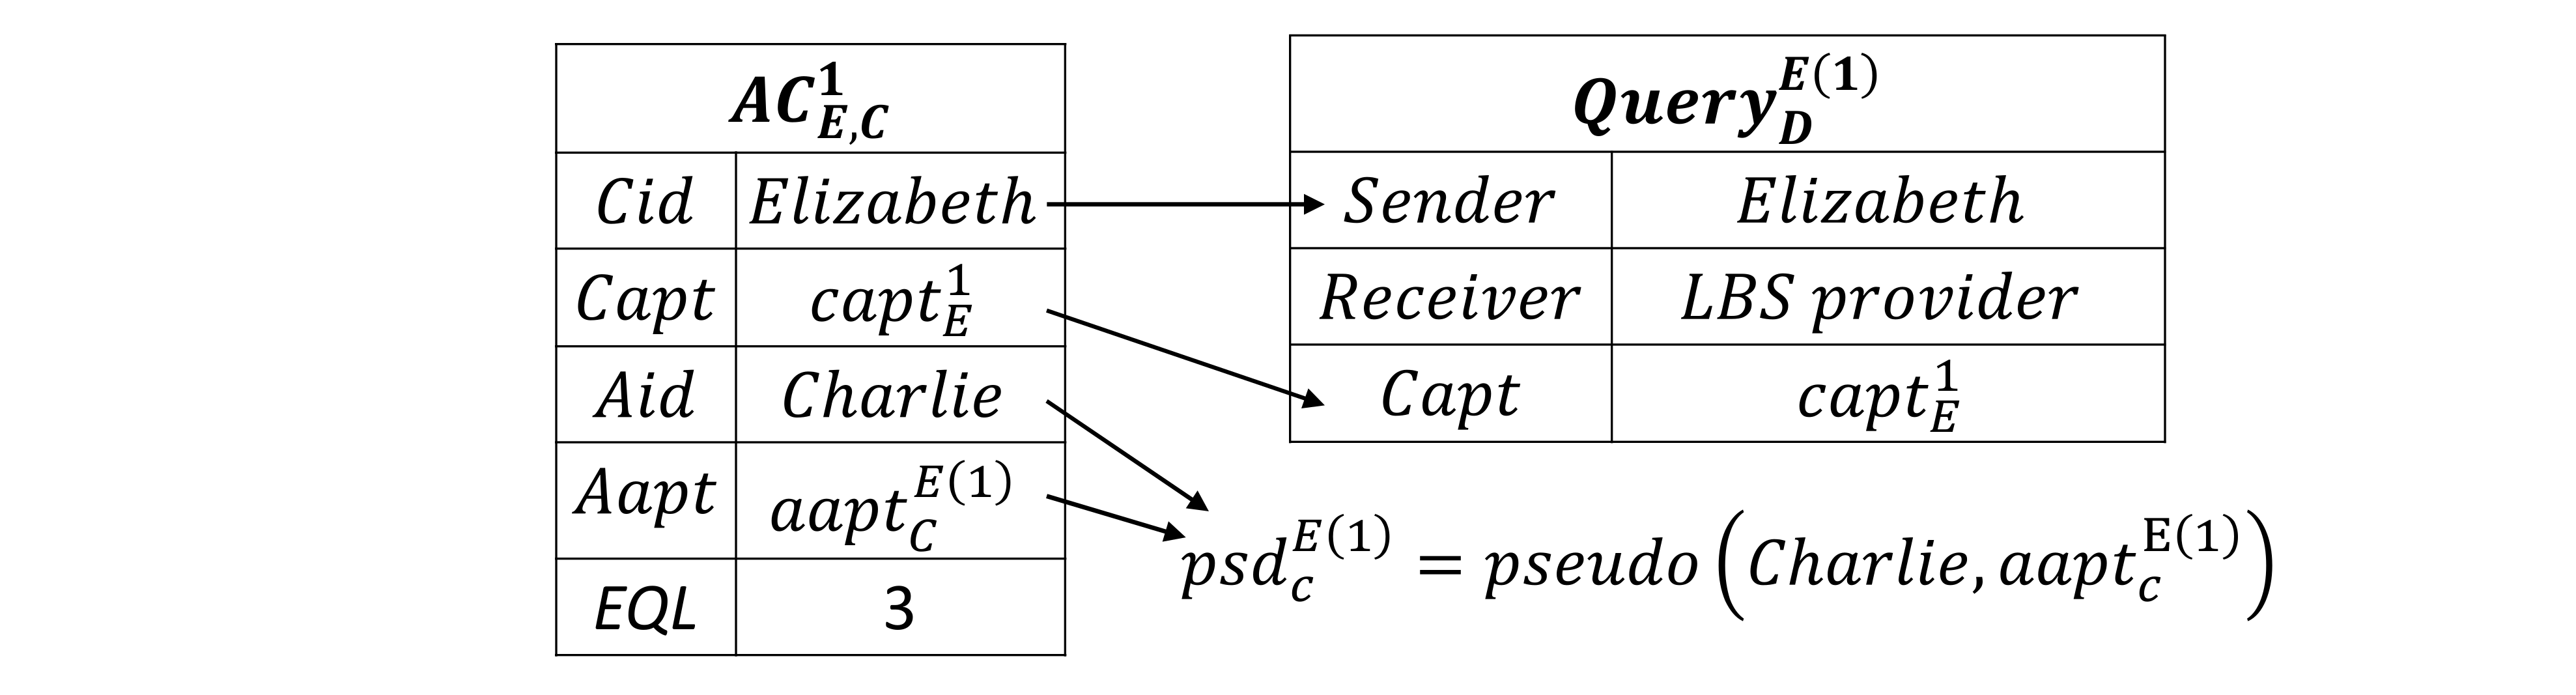
\includegraphics[width=6.0in]{figures/FIG_4_10_Davids_Query.png}
  \caption{David's Query} 
  \label{fig:DavidsQuery} %% label for entire figure 
\end{figure}

The LBS sends a reply message to Elizabeth based on the sender identity of the query. The $Capt$ (i.e., ${capt}^1_E$) is also included in the reply. If an attacker learns these messages, he believes that it is Elizabeth who sends the query.

When Elizabeth receives the reply message, she searches her reply table for the AC used in the reply message, as shown in Table \ref{table:DEReplyTableT8}. Since the message is sent by the LBS, the ${Aid}_{old}$ should equal to her own identity, and the ${Aapt}_{old}$ should equal to the $Capt$. Then she must find an entry like Table \ref{table:ElizabethReplyTableEntry}, which enables Elizabeth to modify the reply message and forward it to Bob, as shown in Figure \ref{fig:ElizabethForwardsAReply}.


\begin{table} [H]
\caption{Elizabeth's Reply Table Entry}
\label{table:ElizabethReplyTableEntry}
\centering
\tabulinesep = 1mm
\begin{tabu}{|c|c|c|c|c|} \hline
${Aid}_{old}$ & ${Aapt}_{old}$ & ${ID}_{nxt}$ & ${Aapt}_{new}$ & \textit{EQL} \\ \hline
$E$ & ${capt}^1_E$ & $B$ & ${aapt}^{E\left(1\right)}_E$ & 1 \\ \hline 
\end{tabu}
\end{table}

\begin{figure} [H]
  \centering 
  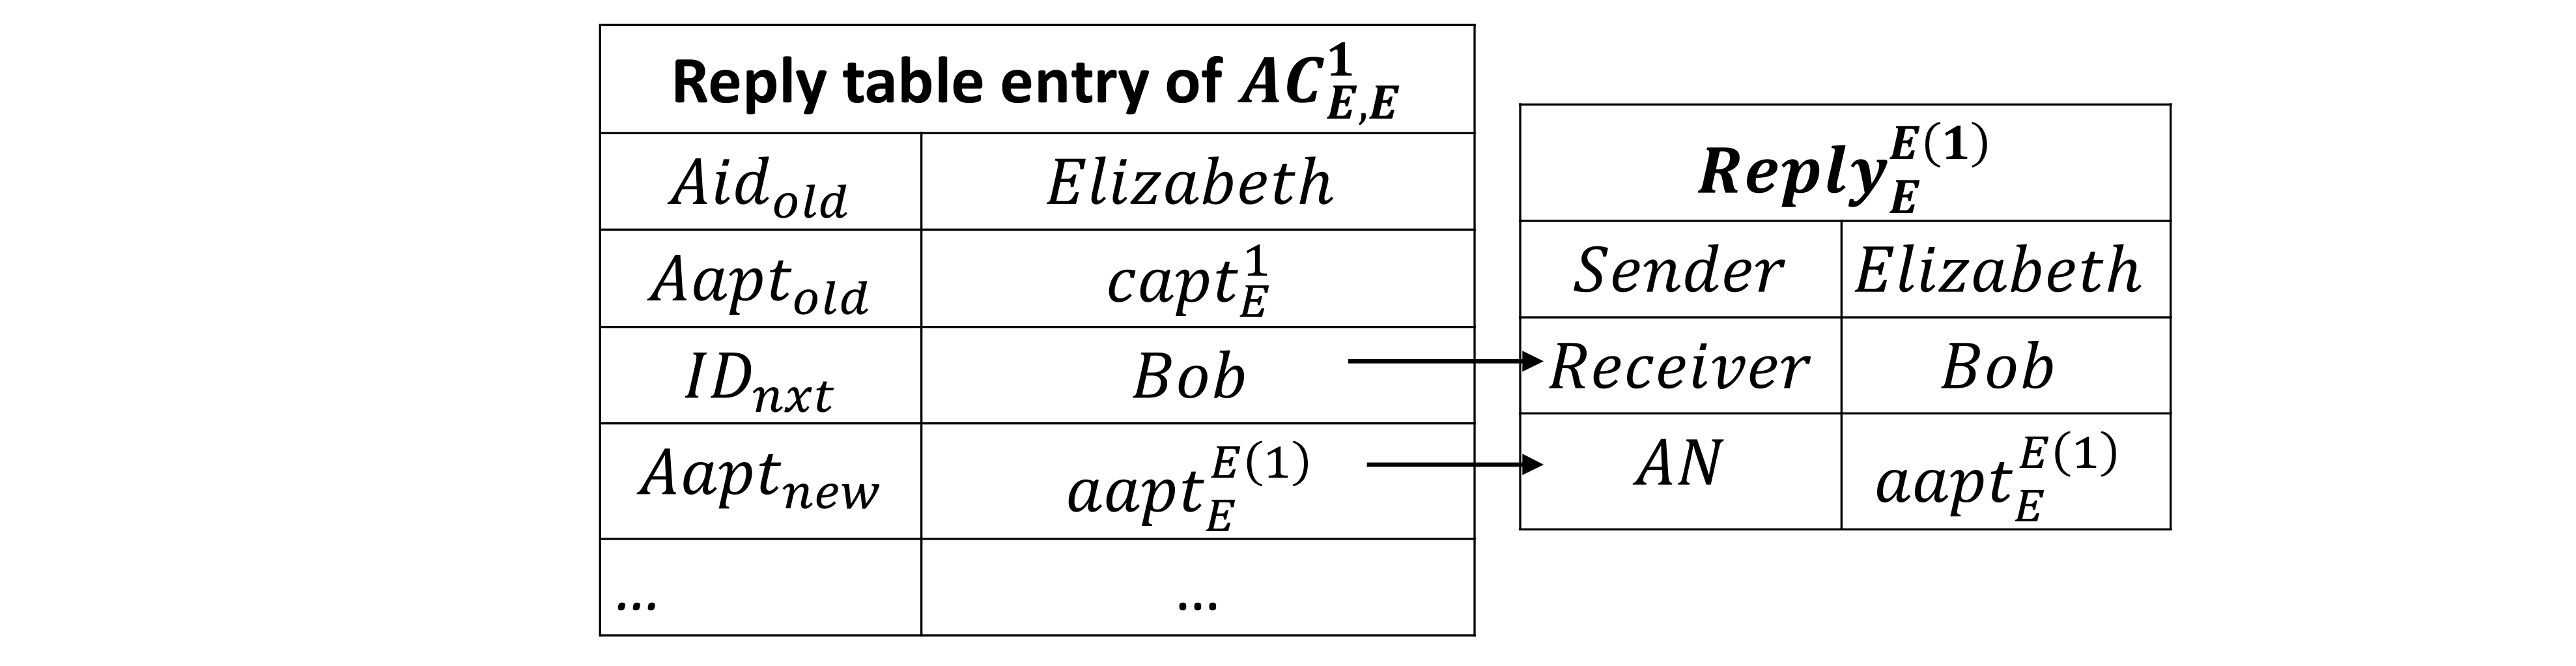
\includegraphics[width=6.0in]{figures/FIG_4_11_Elizabeth_Forwards_A_Reply.png}
  \caption{Elizabeth Forwards A Reply} 
  \label{fig:ElizabethForwardsAReply} %% label for entire figure 
\end{figure}

If Bob receives the reply message successfully, he checks his reply table as shown in Table \ref{table:BCReplyTableT5}. He finds an entry whose ${Aid}_{old}$ is equal to Elizabeth and ${Aapt}_{old}$ is equal to ${aapt}^{E\left(1\right)}_E$, as shown in Table \ref{table:BobsReplyTableEntry}. In the same way as Elizabeth, Bob forwards the reply message to Charlie, as shown in Figure \ref{fig:BobForwardsAReply}.

\begin{table} [H]
\caption{Bob's Reply Table Entry}
\label{table:BobsReplyTableEntry}
\centering
\tabulinesep = 1mm
\begin{tabu}{|c|c|c|c|c|} \hline
${Aid}_{old}$ & ${Aapt}_{old}$ & ${ID}_{nxt}$ & ${Aapt}_{new}$ & \textit{EQL} \\ \hline
$E$ & ${aapt}^{E\left(1\right)}_E$ & $C$ & ${aapt}^{E\left(1\right)}_B$ & 2 \\ \hline 
\end{tabu}
\end{table}

\begin{figure} [H]
  \centering 
  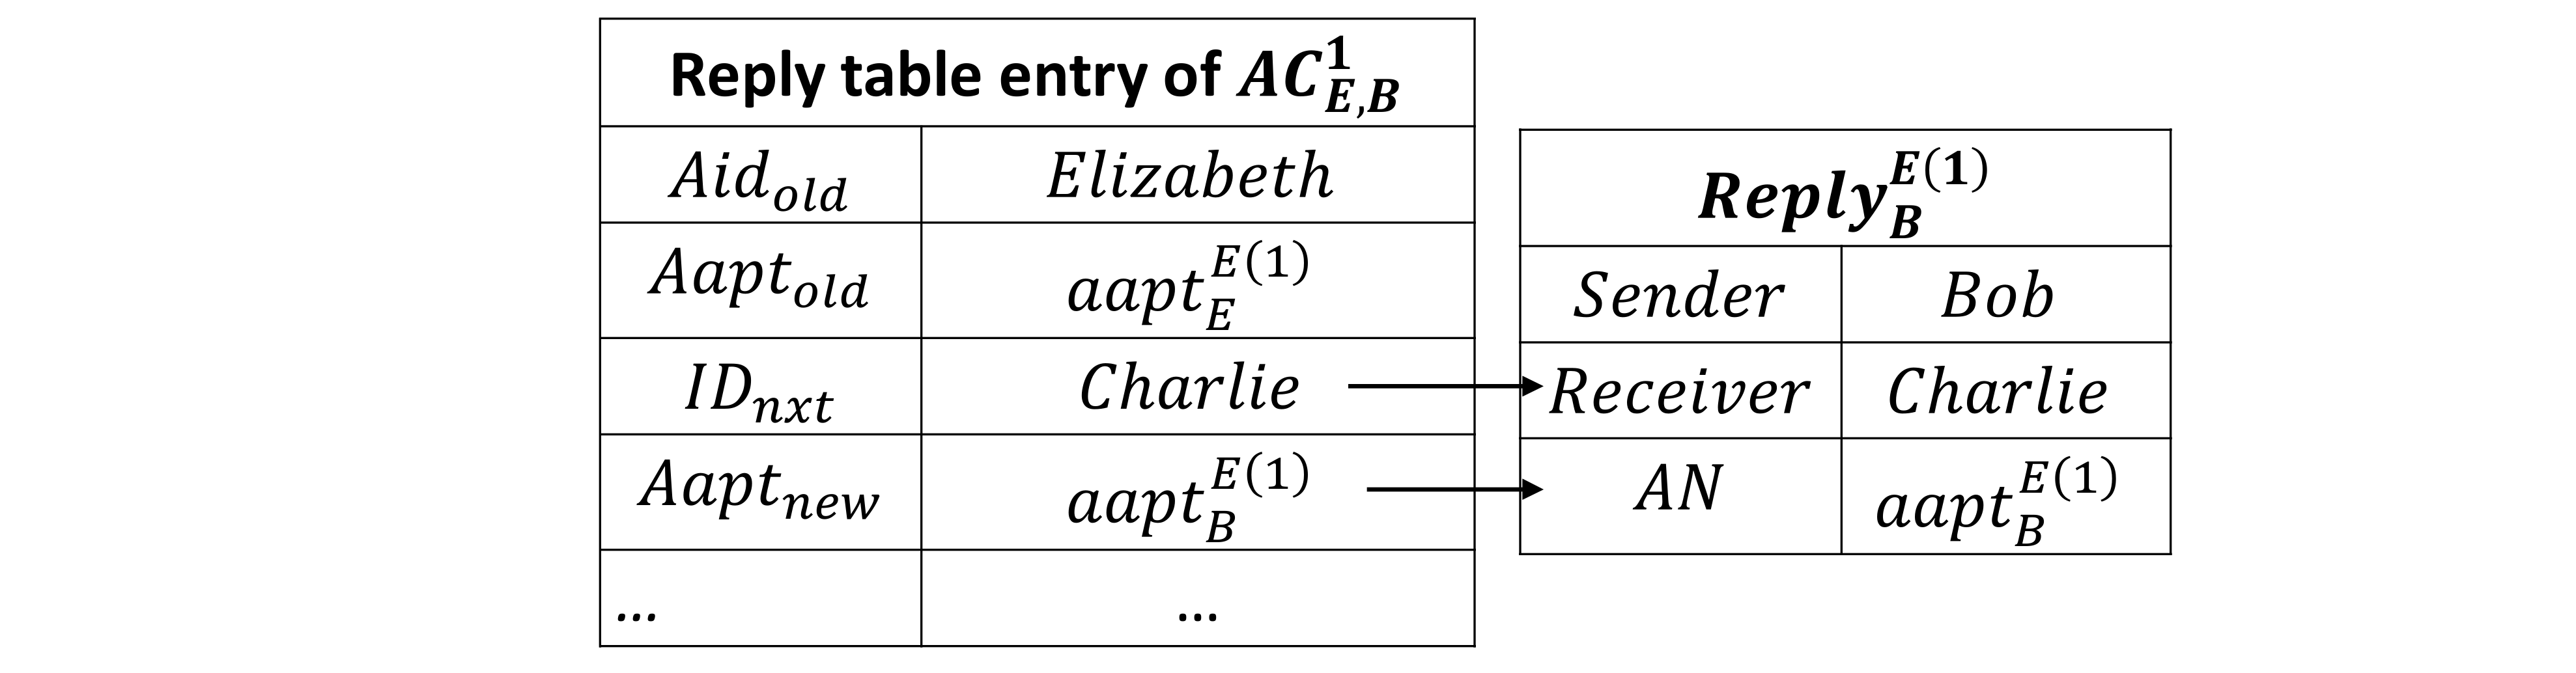
\includegraphics[width=6.0in]{figures/FIG_4_12_Bob_Forwards_A_Reply.png}
  \caption{Bob Forwards A Reply} 
  \label{fig:BobForwardsAReply} %% label for entire figure 
\end{figure}

When the Charlie receives the reply message from Bob, Charlie learns that he is the last agent based on his reply table as shown in Table \ref{table:CDReplyTableT7} and Table \ref{table:CharliesReplyTableEntry}, because the \textit{EQL} is equal to 3. He ignores the record of ${ID}_{nxt}$ $D$ and views it as a $VOID$ because he is the last agent.


\begin{table} [H]
\caption{Charlie's Reply Table Entry}
\label{table:CharliesReplyTableEntry}
\centering
\tabulinesep = 1mm
\begin{tabu}{|c|c|c|c|c|} \hline
${Aid}_{old}$ & ${Aapt}_{old}$ & ${ID}_{nxt}$ & ${Aapt}_{new}$ & \textit{EQL} \\ \hline
$B$ & ${aapt}^{E\left(1\right)}_B$ & $D$($VOID$) & ${aapt}^{E\left(1\right)}_C$ & 3 \\ \hline 
\end{tabu}
\end{table}



To forward the reply message to the unknown original requester (i.e., David), Charlie generates a pseudonym ${psd}^{E\left(1\right)}_c=\mathrm{pseudo}\left(Charlie,{aapt}^{\mathrm{E}\left(1\right)}_c\right)$ using his own identity and ${Aapt}_{new}$. We should notice that the pseudonym is exactly the temporary identity of David. David then modifies the reply message and forwards it, as shown in Figure \ref{fig:CharlieForwardsAReply}.

\begin{figure} [H]
  \centering 
  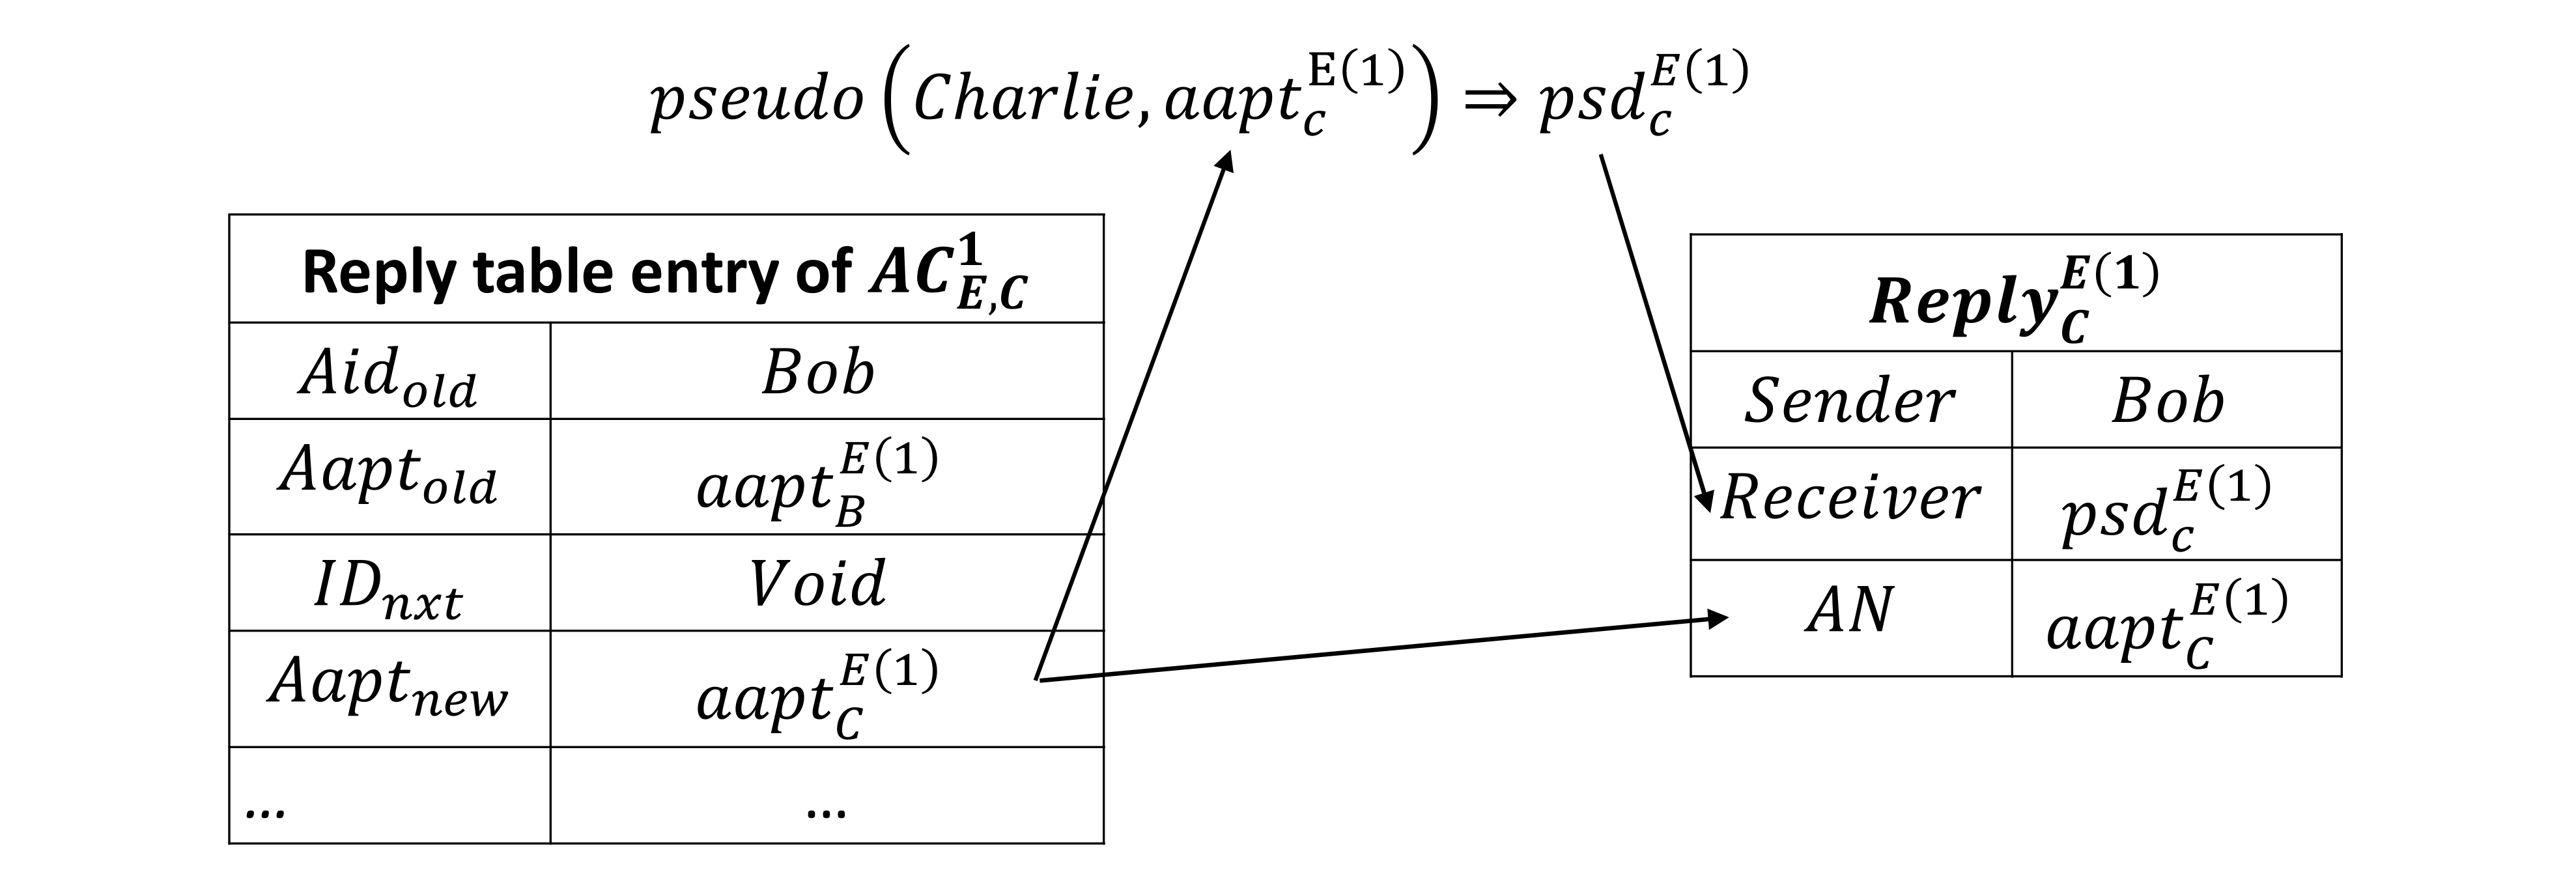
\includegraphics[width=6.0in]{figures/FIG_4_13_Charlie_Forwards_A_Reply.png}
  \caption{Charlie Forwards A Reply} 
  \label{fig:CharlieForwardsAReply} %% label for entire figure 
\end{figure}

When a user who carries ${Reply}^{E\left(1\right)}_C$ encounters David, the user forwards the reply to him, so that David gets his reply.



\section{ Experiment}

\noindent We used the map of Helsinki in our simulator to evaluate the performance of the proposed ACP. We also compare it to Binary Spray and Wait (BSW) protocol \cite{C31}, distributed social based location privacy protocol (SLPD) \cite{C16} and our Multi-Hop Location-Privacy Protection (MHLPP). We simulated the continuous movement of users along streets on the map with one LBSP, fixed at a random location on the map.

For each user, we associate a random social value between 0 - 100\%, each corresponding to other users. Since each social value is assigned with equal probability, we can compute the expected number of friends of a user. If a user whose social value is larger than 85\% is called a friend and there are \textit{n} users in the network, there are $n\times \left(1-85\%\right)$ friends.

The Shortest Path Map-Based Movement (SPMBM) \cite{C35} is used in our experiment. For each experiment, we give the simulator a random seed so that it can generate a pseudo-random number based on the seed. Therefore, all the factors including users' speed and locations are the same if two experiments have the same random seed. All four protocols are tested using the same set of random seeds.

Before each experiment, the simulator runs for 800 seconds (simulator time). Then we pick 100 users out of 126 users randomly, and each of them sends a query to the LBSP. Tests last for about 20 minutes (simulator time). 


\subsection{  Average Query Success Ratio}

\noindent The query success ratio is the percentage of delivered queries among some attempts. Since users sending 100 queries in each experiment, if $s$ queries are delivered to the LBSP at time $t$, the query success ratio of time $t$ is $s\%$.

As shown in Figure \ref{fig:AverageQuerySuccessRatio10}, we compare the average query success ratio of the four protocols with 5 kinds of communication radius (10, 30, 50, 70 and 90 meters). We observe that the ACP and the BSW get a high query success ratio, while the MHLPP and the SLPD are lower than the previous two protocols. The BSW is the highest one because it is a no-privacy protocol. The ACP is just a little lower than BSW, because the query delivery process of the ACP is almost the same as that of BSW. Since users of ACP must wait for available appointment cards, they cost more time to initial their queries. However, the ACP and the BSW are at the same level, comparing to the other two protocols. The MHLPP and the SLPD need to find friends to obfuscate their queries, which baffles their delivery process.

\begin{figure} [H]
  \centering 
  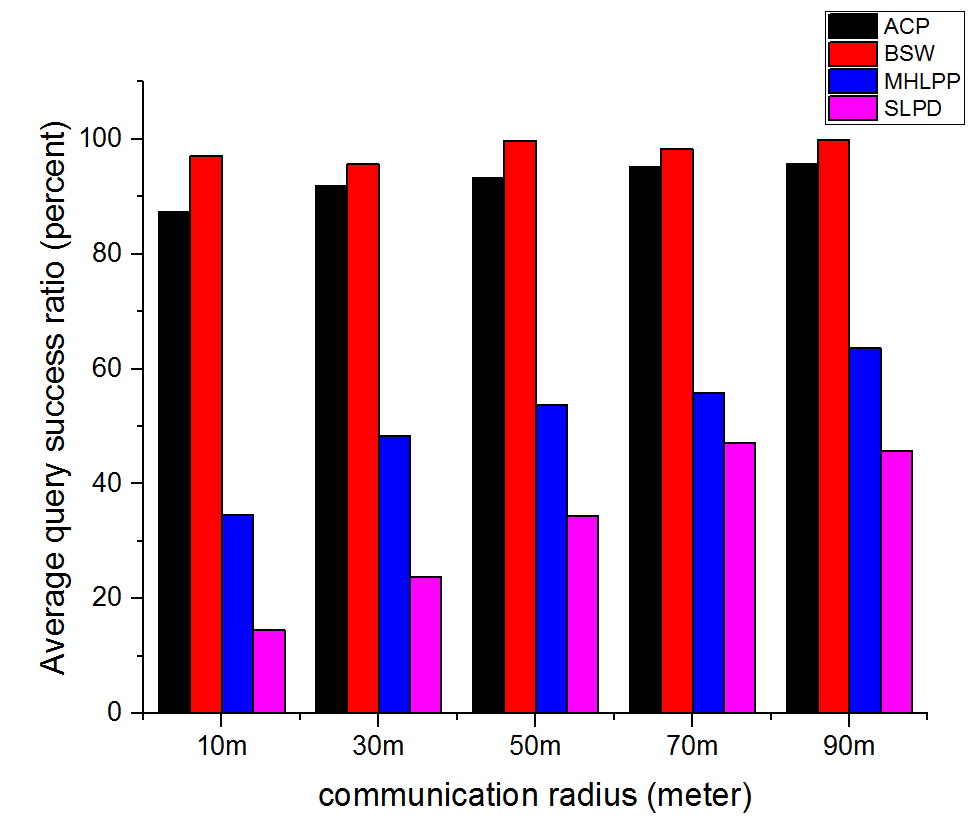
\includegraphics[width=4.0in]{figures/F414AverageQuerySuccessRatio10minutes.png}
  \caption{Average Query Success Ratio (10 minutes)} 
  \label{fig:AverageQuerySuccessRatio10} %% label for entire figure 
\end{figure}

The experiment results when we test 20 minutes is shown in Figure \ref{fig:AverageQuerySuccessRatio20}. Comparing to the average query success ratio at 10 minutes, the MHLPP and the SLPD achieve much higher success ratio after 20 minutes than at 10 minutes. That is because it cost them so much time in their obfuscation phases when they need to find friends. In fact, some of the queries of the MHLPP and the SLPD still do not finish their obfuscation phase at 20 minutes.

\begin{figure} [H]
  \centering 
  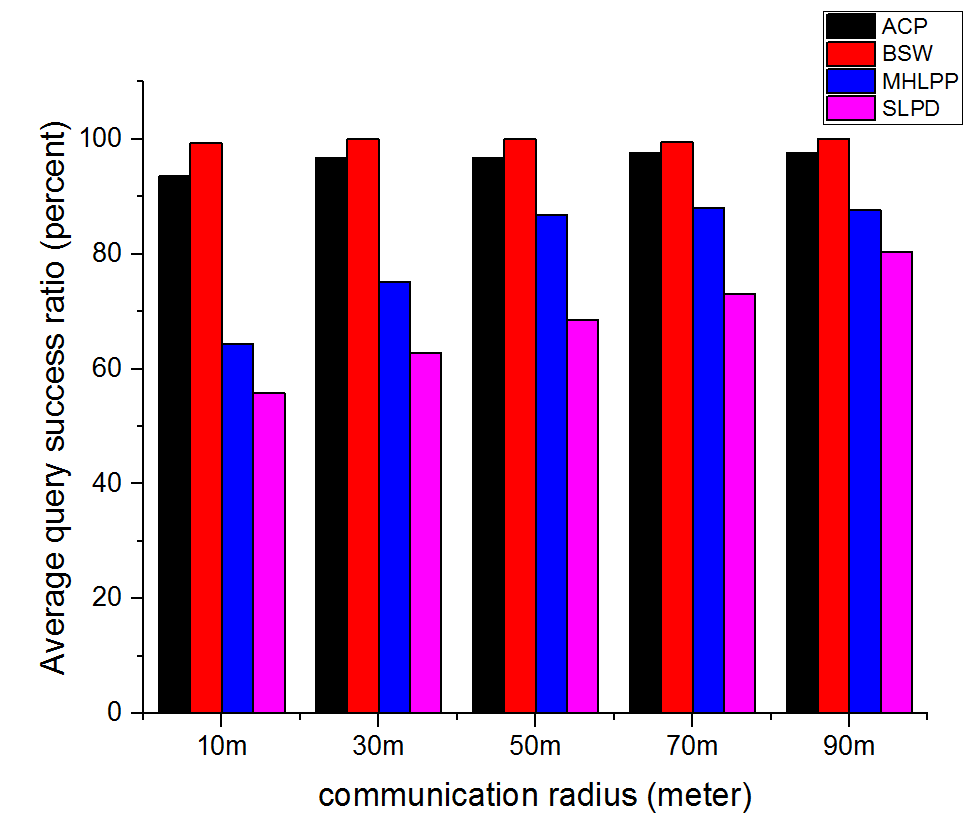
\includegraphics[width=4.0in]{figures/F415AverageQuerySuccessRatio20minutes.png}
  \caption{Average Query Success Ratio (20 minutes)} 
  \label{fig:AverageQuerySuccessRatio20} %% label for entire figure 
\end{figure}

The communication radius can influence the success ratio. In most of the cases, the success ratio rises when we increase the communication radius, and its influence is especially evident under 50 meters. A large communication radius makes it easy for users to encounter others, which is good for them to forward queries. However, a user who is so far away from the destination does not want the intermediates of his query encounters many users nearby. Because all users who carry copies of that query are near the sender instead of the destination, which decreases their query success ratio. Therefore, when the communication radius reaches 70 meters, the success ratios almost stay at the same level.

In Figure \ref{fig:F416AverageQuerySuccessRatioWith50MetersCommunicationRatio}, we observe that the ACP and the BSW have better convergence speed than the MHLPP and the SLPD. In other words, the former two protocols have a faster speed to approach the 100\% query success ratio than the latter two. At the very beginning, the ACP even has a little higher success ratio than the BSW. Because the ACP users need ready appointment card, and most of the users get their first ready appointment cards at places where there are many users. Therefore, users rarely generate query near the edges of the map at the beginning, which facilitates their queries delivery process. For example, if a user generates his query at the edge of the map, the copies of this query might be sent to users who are also at the edge, and it takes more time for them to deliver the query. If the user does not generate his query until he arrives a place nearer the center, the copies of this query will be carried by the users in the center with higher probability.

\begin{figure} [hbtp]
  \centering 
  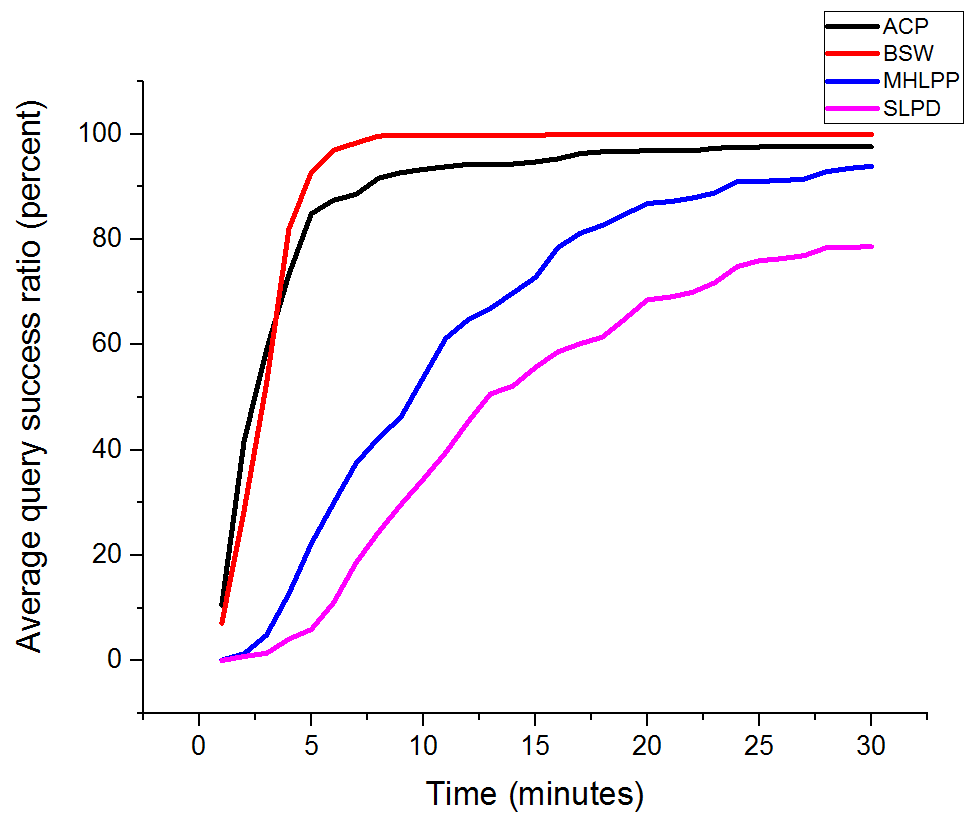
\includegraphics[width=4.0in]{figures/F416AverageQuerySuccessRatioWith50MetersCommunicationRatio.png}
  \caption{Average Query Success Ratio With 50-Meters Communication Ratio} 
  \label{fig:F416AverageQuerySuccessRatioWith50MetersCommunicationRatio} %% label for entire figure 
\end{figure}

\subsection{ Average Reply Success Ratio}

\noindent When the LBSP receives a query, it sends a reply to the requester. If the reply arrives the original requester before the test ends, we view it as a success; otherwise, the reply is failed. There are two reasons for the failure of replies: 1) the query is not delivered to the LBSP successfully; 2) the query costs too much time so that the reply has no time to be delivered; 3) The route of the reply is too long. Since there are 100 queries in each experiment, the number of replies should be equal to 100. 

In Figure \ref{fig:F417AverageReplySuccessRatioWith50MetersCommunicationRatio}, the BSW has a significant and reasonable higher success ratio than all other protocols, because it is a no-privacy protocol. The ACP is higher than the MHLPP and the SLPD, but its advantage is not as large as that in the query process. In fact, the reply process of the MHLPP and the SLPD are simpler than that of the ACP, but the ACP saves so much time in its query process that it earns a better reply success ratio than the other two.

\begin{figure} [hbtp]
  \centering 
  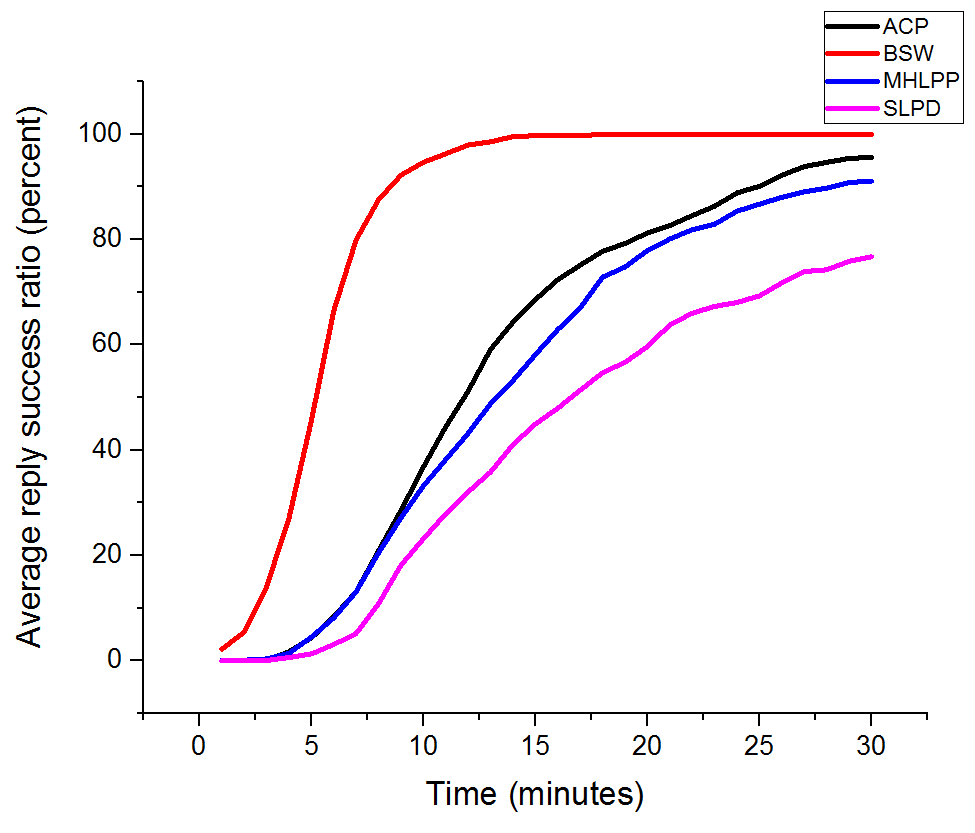
\includegraphics[width=4.0in]{figures/F417AverageReplySuccessRatioWith50MetersCommunicationRatio.png}
  \caption{Average Reply Success Ratio With 50-Meters Communication Ratio} 
  \label{fig:F417AverageReplySuccessRatioWith50MetersCommunicationRatio} %% label for entire figure 
\end{figure}

\subsection{ Total Number of Query Relays}

\noindent The query delivery processes of all the four protocols use the BSW protocol, and the BSW makes copies for queries and gives half of the copies to any users it encounters. That is a significant cost for the network, so we use the number of query relaying (QR) to evaluate that cost. The QR is initialized as zero at the beginning of the test. When a user relay a (or several) copies of a query, we increase QR by 1. For example, in the SLPD, there are two phases: the obfuscation phase and the free phase. In the obfuscation phase, a query is forwarded among one-hop friends for $k$ times. After that, it is forwarded by the BSW protocol. The BSW protocol makes $c$ copies of the query and gives half of the copies to any encountering users. Then QR should be about $k+c$. Since a user gives all its copies to the destination if he encounters the destination at once, the QR may be smaller. The smaller that number is, the smaller cost of the network is. Since there are 100 queries, we divide QR by 100 to get an average value. 

In Figure \ref{fig:F418AverageTotalNumberofForwardingQueriesAt20Minutes}, we compare QR with four protocols. We observe that all the four protocols are at a similar level, the BSW and the ACP is a little lower than the other two. For the ACP and the BSW, they deliver queries so fast that users who carry more than one copies give all their copies to the destination before they send these copies to different users separately. As a result, many copies have no chance to be forwarded, which decreases the cost. While the MHLPP and the SLPD have obfuscation phases, the queries start to be delivered freely (in a BSW way) at a random place where might be so far away from the destination, so that almost all copies can be forwarded respectively.

\begin{figure} [hbtp]
  \centering 
  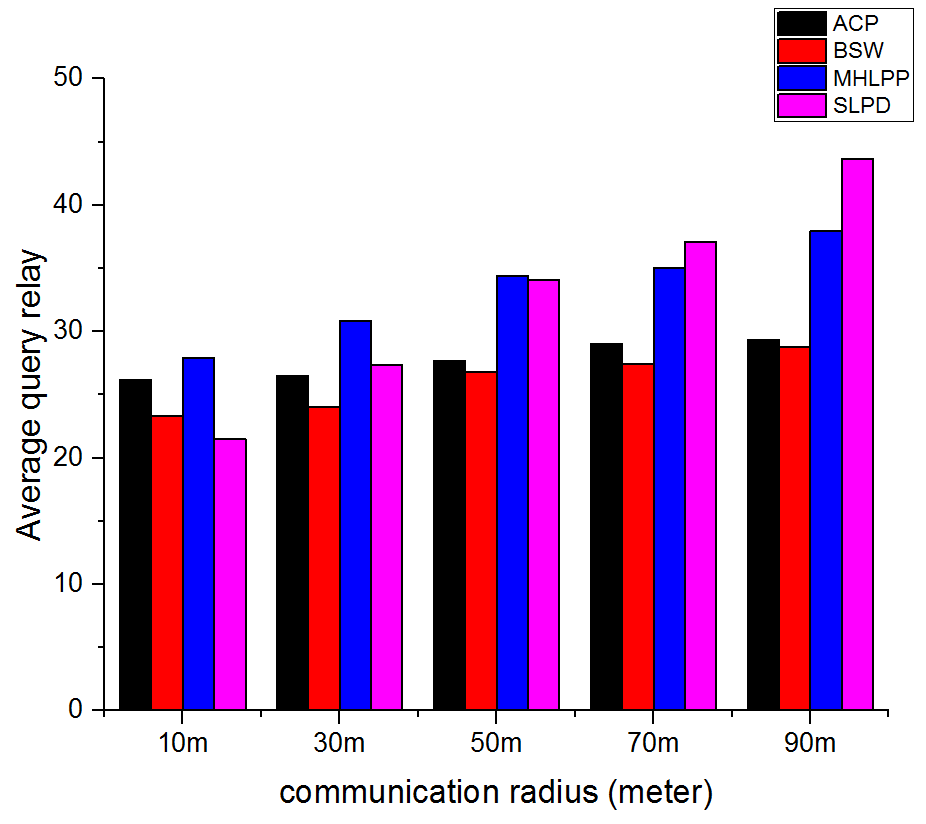
\includegraphics[width=4.0in]{figures/F418AverageTotalNumberofForwardingQueriesAt20Minutes.png}
  \caption{Average Total Number of Forwarding Queries At 20 Minutes} 
  \label{fig:F418AverageTotalNumberofForwardingQueriesAt20Minutes} %% label for entire figure 
\end{figure}

The communication radius affects the total number of the forwarding queries, especially for the MHLPP and the SLPD. Those two protocols can finish their obfuscation phase more quickly which a larger communication radius, so that more queries can be forwarded freely (in the BSW way), which makes their QR larger.

\subsection{ Memory Cost}

\noindent We count the number of queries carried by each user to evaluate the memory cost of the four protocols. Several copies of a query are counted for only once.

In the Figure \ref{fig:F419AverageQueryBufferNeededAt20Minutes}, we compare the number of queries per user with the four protocols at 20 minutes. We observe that the BSW is the highest in most of the cases and the ACP always stays at a similar level as the BSW. The data of other two protocols (the MHLPP and the SLPD) increase as the communication radius. The MHLPP even excesses the BSW when the communication radius is 90 meters. The reason is that quite a number of the BSW and the ACP users forward their copies to the destination so that there is no copy with them at 20 minutes, while the rest of them cannot forward their copies to the destination even given a large communication radius. At the same time, the number of the other two protocol's free phase queries is significantly influenced by the communication radius. The more queries are in the free phase; the more copies are in the network.

\begin{figure} [hbtp]
  \centering 
  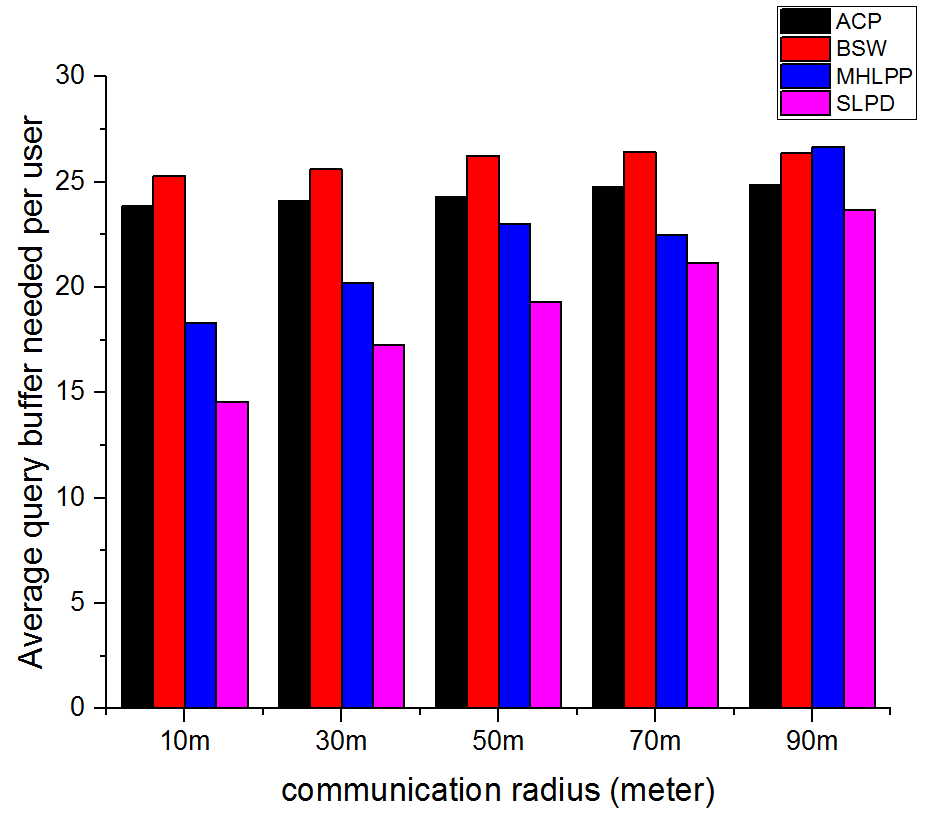
\includegraphics[width=4.0in]{figures/F419AverageQueryBufferNeededAt20Minutes.png}
  \caption{Average Query Buffer Needed At 20 Minutes} 
  \label{fig:F419AverageQueryBufferNeededAt20Minutes} %% label for entire figure 
\end{figure}

The Figure \ref{fig:F420AverageNumberofCarriedQueriesPerUser} shows the average number of queries which are carrying by users when the communication radius is 10, 50 and 90 meters. The curves of the ACP and the BSW rise sharply at the beginning and then become flat, while those of the MHLPP and the SLPD rise smoothly and continuously. 

\begin{figure} [hbtp]
  \centering 
  \subfigure[communication radius is equal to 10 meters]{ 
    \label{fig:F420AverageNumberofCarriedQueriesPerUser:a} %% label for first subfigure 
    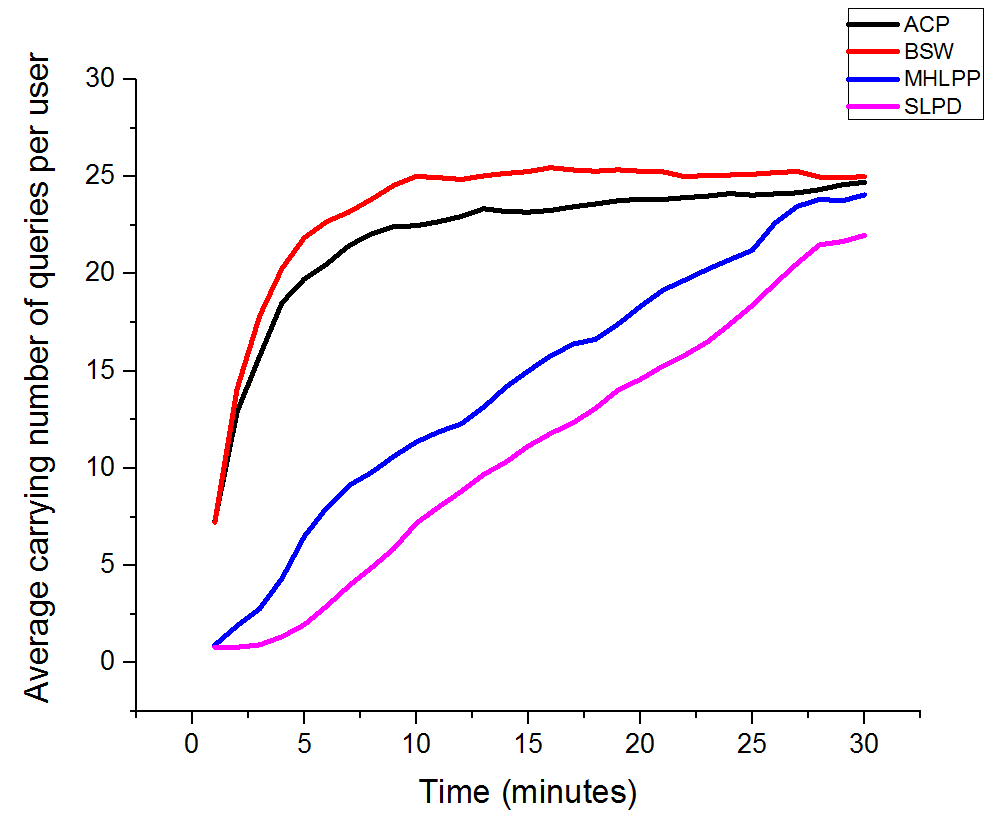
\includegraphics[width=3.0in]{figures/F420AverageNumberofCarriedQueriesPerUser10.png}} 
  \hspace{1in} 
  \subfigure[communication radius is equal to 50 meters]{ 
    \label{fig:AverageNumberofCarriedQueriesPerUser:b} %% label for second subfigure 
    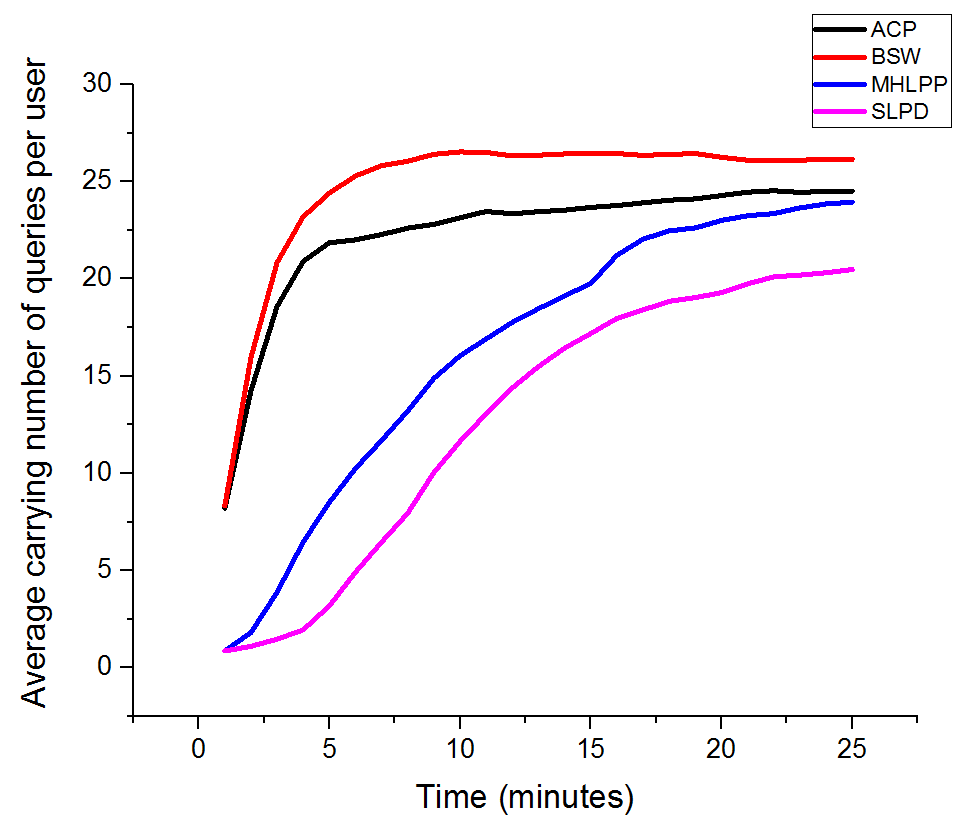
\includegraphics[width=3.0in]{figures/F420AverageNumberofCarriedQueriesPerUser50.png}}
  \hspace{1in} 
  \subfigure[communication radius is equal to 90 meters]{ 
    \label{fig:AverageNumberofCarriedQueriesPerUser:c} %% label for second subfigure 
    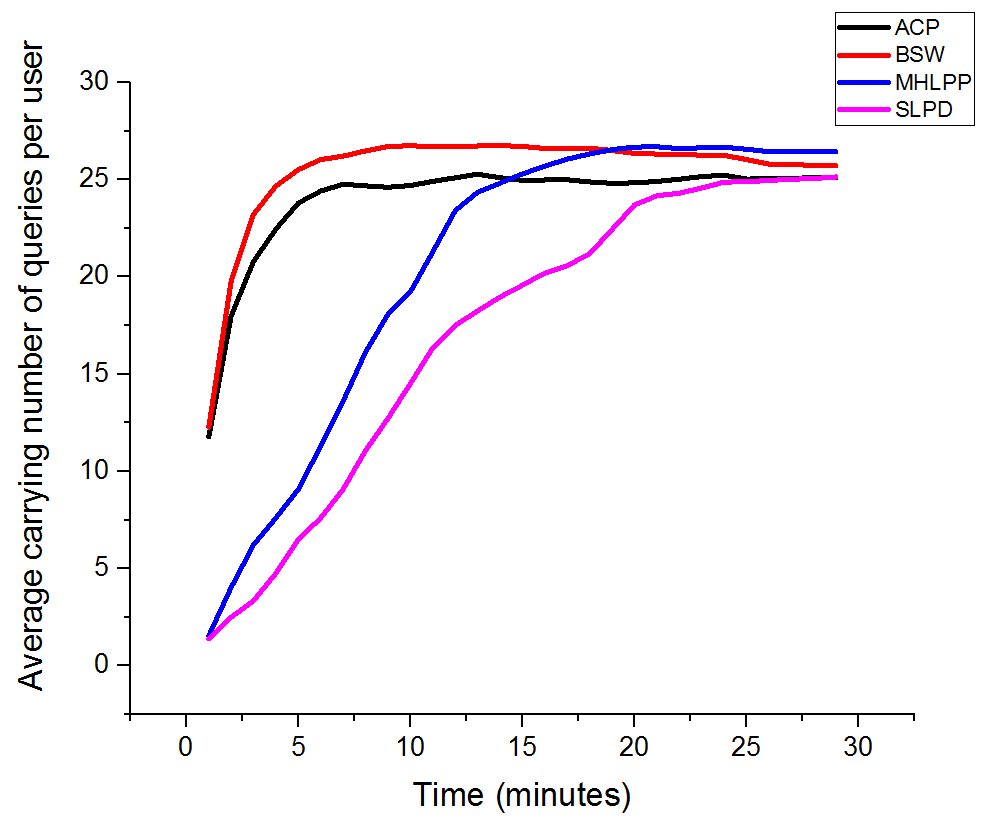
\includegraphics[width=3.0in]{figures/F420AverageNumberofCarriedQueriesPerUser90.png}}
  \caption{Average Number of Carried Queries Per User} 
  \label{fig:F420AverageNumberofCarriedQueriesPerUser} %% label for entire figure 
\end{figure}

\subsection{ Distributing Appointment Cards}

\noindent Exchanging appointment cards is a feature of the ACP, which imports burden into the network. We count the number of exchanging appointment cards per minute to evaluate the extra cost of the ACP.

In Figure \ref{fig:F422AverageNumberofExchangingACsPerMinute}, we count the total number of exchanging ACs in the whole network. For example, if a user Alice encounters another user Bob, the total of exchanging ACs processes increases by one when Alice exchanges any ACs to Bob. We count the number of those exchanging processes occur per minute. As shown in the figure, the exchanging processes do not occur frequently, but about 2 times per minutes. Since the size of an appointment card is small, it does not cost the network many resources. At the same time, users can get many appointment cards to help them send queries, as shown in Figure \ref{fig:F421AverageNumberofReadyACsPerUser}. The number of ready ACs per user is raising smoothly and steadily. 

\begin{figure} [hbtp]
  \centering 
  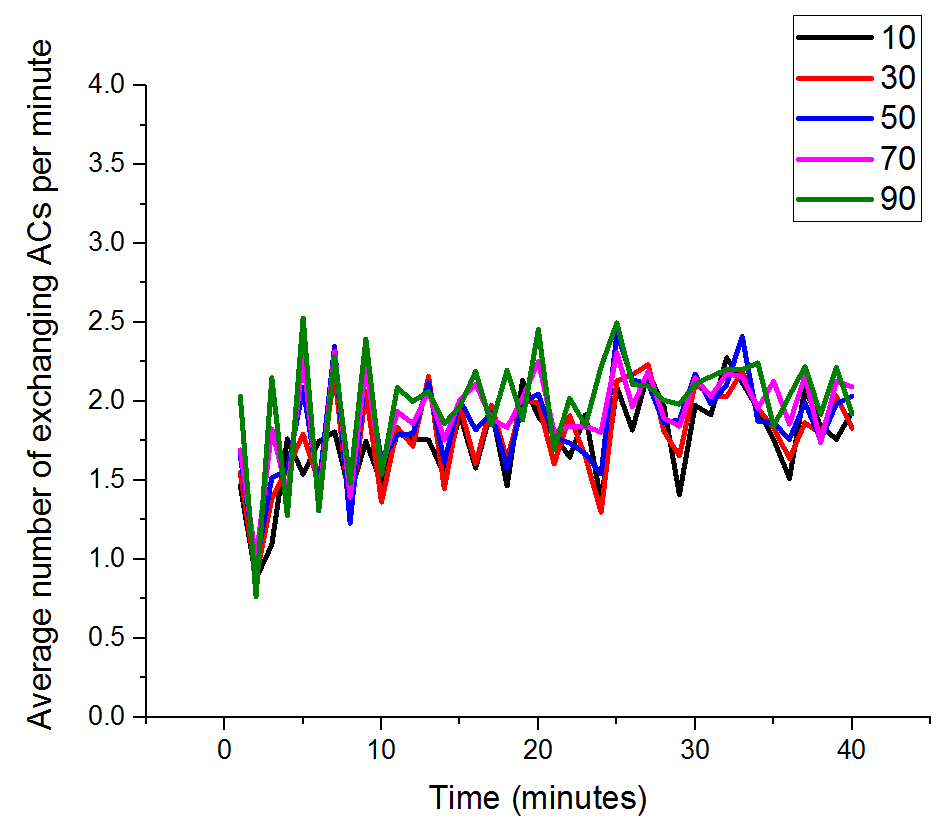
\includegraphics[width=4.0in]{figures/F422AverageNumberofExchangingACsPerMinute.png}
  \caption{Average Number of Exchanging ACs Per Minute} 
  \label{fig:F422AverageNumberofExchangingACsPerMinute} %% label for entire figure 
\end{figure}

\begin{figure} [hbtp]
  \centering 
  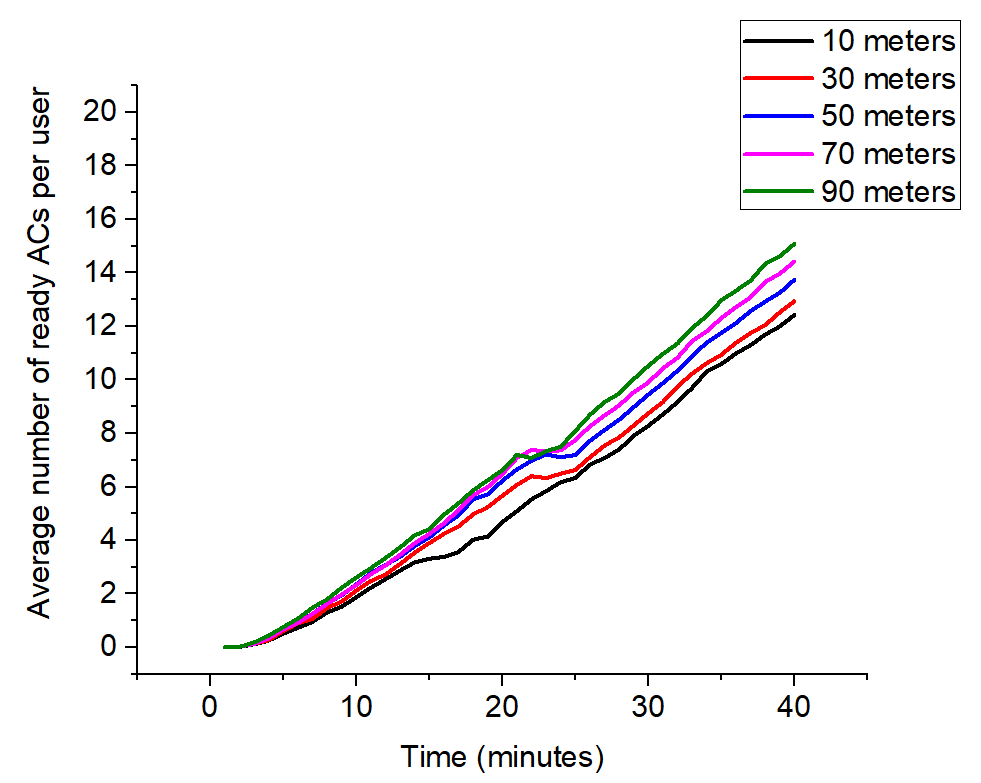
\includegraphics[width=4.0in]{figures/F421AverageNumberofReadyACsPerUser.png}
  \caption{Average Number of Ready ACs Per User} 
  \label{fig:F421AverageNumberofReadyACsPerUser} %% label for entire figure 
\end{figure}






%%%%%%%%%%%%%%%%%%%%%%%%%%%
\chapter{OMSN Routing Simulator (ORS)}
\label{OPS}
%%%%%%%%%%%%%%%%%%%%%%%%%%%

\noindent The Opportunistic Networking Environment (ONE) \cite{C35} is a simulator designed for evaluating DTN routing and application protocols. Researchers can import real-world map into the simulator so that hosts walk along streets and roads in the simulator. The movement model of hosts can be defined by researchers, which enables researchers to evaluate the performance of their protocols in different scenarios. The User Interface of the ONE is also friendly, where researchers can observe the movement of all hosts. When a round of experiment ends, ONE outputs the results to a defined file. The simulator can also execute in console mode, which allows a higher experiment speed.

The ONE is an excellent simulator for DTN research, while it has its own weakness. The way that ONE estimates the distance between two hosts is not thorough, which may lead to inaccurate results. When a host broadcasts a message, only the hosts which are in its communication radius should receive the message. If the simulator cannot give the accurate set of hosts which can receive the message, the experiment result is not reliable. Although we can avoid this problem by setting parameters carefully, this problem cannot be completely ignored. Besides, some movement models need to calculate shortest path several times, which may require several seconds. Even though that is not a long time, it can slow down the experiment speed significantly as the total time of a round of experiment is about 10-20 seconds. 

In this chapter, we introduce two major algorithms used in our new ORS simulator. The vertex reduce algorithm is used for simplifying the input of the all-pair shortest path algorithm, so that the simulator can initialize quickly. The finding nodes algorithm is used to find users which are in the communication radius of a given user.

\section{Overview}
At its core, ORS is a discrete event simulation engine. To simulate an OMSN, hosts can move in the simulator, and information of social network is also included in the simulator. The simulator reads real-world maps, which enables hosts to walk along streets on the maps. The default movement model of hosts is Working day movement model \cite{C32} where hosts walk through the shortest path between several random points. Researchers can replace the movement model with other models by implementing models in the source codes.

The main function of ORS can be considered as the movement of hosts and message routing. The movement routes of hosts is generated based on the movement model and are defined by a series of segment lines before the simulation starts. In other words, the routes are fixed before hosts start to walk so that the locations of hosts is a function of time. Since ORS can get the locations of hosts directly when given a specific time value, it only calculate locations of hosts when some hosts send messages or UI needs the locations of hosts. Each host has a communication range which is a circle. ORS calculates the locations of hosts when one or more hosts send messages, and the hosts inside the communication range must receive the sent messages. The messages are always broadcast, and ORS copies them to all hosts inside the communication range of the host who sends the message. Therefore, the host itself decides whether a received message should be received or not, which enables the hosts to control as many details as possible. The message structures are defined by the implementation of DTN routing protocols and do not have mandatory entries except a unique ID assigned by the simulator which is used for identifying messages. 

The UI of ORS is shown in Figure \ref{fig:SimulatorUI}. The parameters of the simulator which include the file path of the map file, the number of hosts, the communication range and so on are defined in a ``txt'' file. When we use ORS open the ``txt'' file (e.g., ``aenv1.txt''), ORS reads all parameters in the file and initialize the simulator. First, the simulator draws the map and uses yellow lines to denotes the streets; second, ORS generates hosts, their relationship strength, and their movement routes; third, ORS initializes instances of a specific routing protocol for each host. ORS starts the experiment automatically when the initializations finish. Users can define the values of the textboxes on the UI in source codes so that they can debug their protocols.

\begin{figure} [hbtp]
  \centering 
  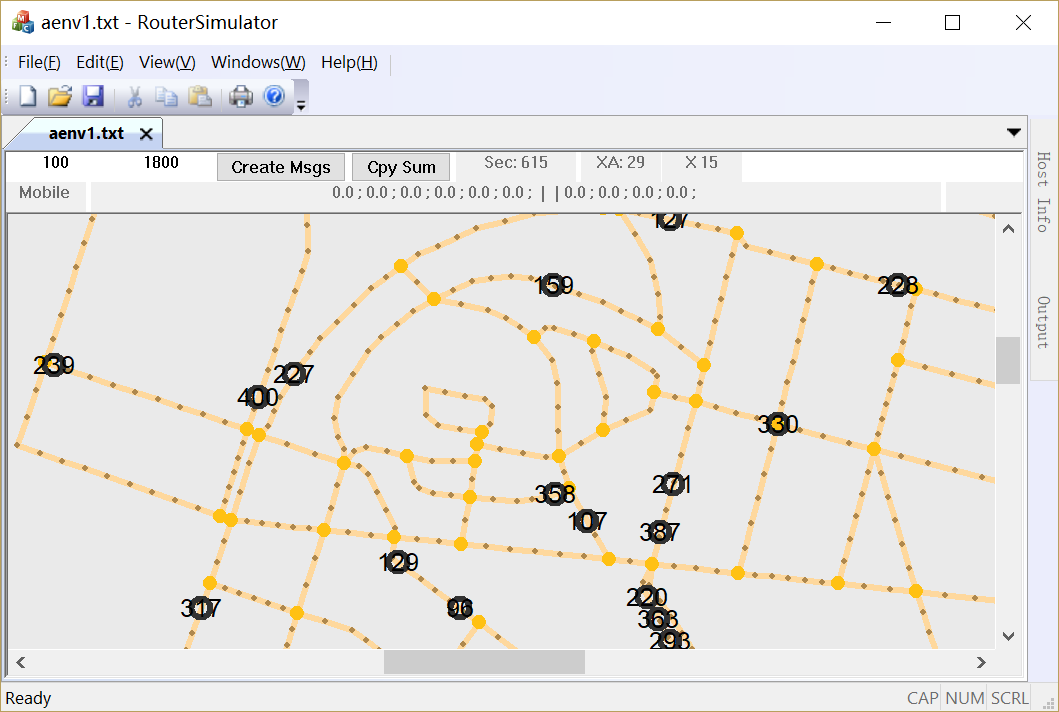
\includegraphics[height=4in]{figures/simulator.png}
  \caption{Simulator UI} 
  \label{fig:SimulatorUI} %% label for entire figure 
\end{figure}

The hosts in the simulator can be viewed as mobile devices (e.g., smartphones) which are a leak of software. These devices are carried by people who are moving in the simulator. ORS offers the devices interfaces so that users can implement routing protocols which is the software of the mobile devices. The interfaces which devices can get from ORS includes setting timers, current time, the identities of their owners, sending messages to surroundings and so on. Comparing to ONE, the interfaces of ORS are more flexible so that developers can almost define everything when they implement their routing protocols, like the size of buffers or the frequency of sending hello messages. ORS leaves the implementation of persistent storage, energy consumption and message routing to routing protocols instead of giving interfaces of these features, which enables researchers to make their experiments more accurate. For example, the sizes of the messages are different. the hello messages are small while general messages are large. Also, different operations cost different energy. Therefore, it is good for developers to define these features by them self. ORS can track all messages if developers implement the method by which ORS can identify messages. In this way, researchers can learn the location of each message, the number of the message which is delivered to the destination, and the state of each message (e.g., shipping or delivered).

The relationship strengths of each pair of hosts are defined when ORS initials hosts. The relationship strengths are fixed during the experiment. All relationship strengths are recorded in a table so that routing protocols can get the relationship between any pair of hosts when the protocols learn their identities. In general case, the routing protocols can learn the identity of their owners and the identity of the senders of messages, so that routing protocols can get the relationship strengths between the senders and their owners.


\section{Vertex Reduction Algorithm}

\noindent Movement of network nodes is a significant factor in the performance of DTNs. To evaluate the performance of different DTN protocols, researchers have presented different kinds of movement models, like in \cite{C32}. Since shortest path algorithm is an essential and time-cost part of creating many movement models, it is an important aspect to optimize the time-cost for simulators, calculating the all-pairs shortest paths in the entire map.

The best known non-negative edge weight undirected map all-pairs shortest path algorithm \cite{C33} has a complexity $O\left(n^2{\mathrm{log} n\ }\right)$, which is still expensive when \textit{n} is huge. For most real-world city maps, there are thousands of points in a single square kilometer. Since a ten-square kilometers map is reasonable for a DTN protocol evaluation, a simulator must cut down the time spent in calculating all-pairs shortest paths to speed up the experiment.

Real-world map developers often use short straight lines to present curves, like in \cite{C34}, so that a several-meters curves may contain tens of points. It is obvious that we do not need to calculate shortest path for every one of these points. In this chapter, we present an Vertex Reduction Algorithm (VRA) to reduce the number of points before the use of the shortest path algorithm. The basic idea is that VRA removes all points whose degrees are less than 3 from the map, while keeping the result of all-pairs shortest path algorithm correct.

The rest of this chapter is organized as follows. Section \ref{subsecIVRV} presents some basic definitions and lemmas. The process of VRA is described in Section \ref{subsecVR} and Section \ref{subsecAssVer}.



\subsection{ Ignorable Vertex and Reserved Vertex}\label{subsecIVRV}

\noindent Vertices in the graph are considered ignorable and/or reserved (definition follows). In each iteration of VRA, we remove the ignorable vertex from the graph, while the reserved vertices compose a new graph.

\textit{Definition} \textit{1}: The vertex whose degree is larger than 2 is the \textit{reserved} vertex (denoted by $R$).

\textit{Definition} \textit{2}: The vertex whose degree is smaller than or equal to 2 is called the \textit{ignorable} vertex (denoted by $G$).

\textit{Definition} \textit{3}: If two reserved vertices (e.g. $R_1,R_2$) are connected by a sequence of ignorable vertices (e.g. $G_1,G_2,\mathrm{\cdots },G_n$), then the sequence from $R_1$ to $R_2$ (i.e., $R_1,G_1,G_2,\mathrm{\cdots },G_n,R_2$) is a \textit{line-segment} (denoted by $LS$). 

A reserved vertex can belong to different line-segments, while an ignorable vertex belongs to a unique line-segment. Both the reserved vertex and the ignorable vertex are called vertices ($V$)\textit{}

\textit{Definition} \textit{4}: The shortest route between two vertices inside a \textit{segment-line} is called the \textit{inner shortest path} ($SPI$). 

Let ${SPI}\left(V_i,V_j\right)$ denote the inner shortest path between two vertices (i.e., $V_i,V_j$) inside a \textit{segment-line}.

\textit{Lemma} \textit{1}: If two vertices (i.e., $V_i$, $V_j$; $i<j$) are in the same line-segment, the shortest path between them is

\begin{equation} \label{GrindEQ__VRShortestInner} 
{SP}\left(V_i,V_j\right)={min}\left\{SPI\left(V_i,V_j\right),SPI\left(R_1,V_i\right)+SPI\left(V_j,R_2\right)+SP\left(R_1,R_2\right)\right\}
\end{equation}

\textit{Proof}: \textit{Lemma} \textit{1} is shown in Figure \ref{fig:ShortestPathOnASingleSegment}. We assume that there is a path (e.g., $V_i-V_x-V_j$) whose length is smaller than or equal to Equation \ref{GrindEQ__VRShortestInner} between $V_i$, $V_j$, where $V_x$ is a vertice in the \textit{segment-line} including $V_i$, $V_j$.

\begin{figure} [hbtp]
  \centering 
  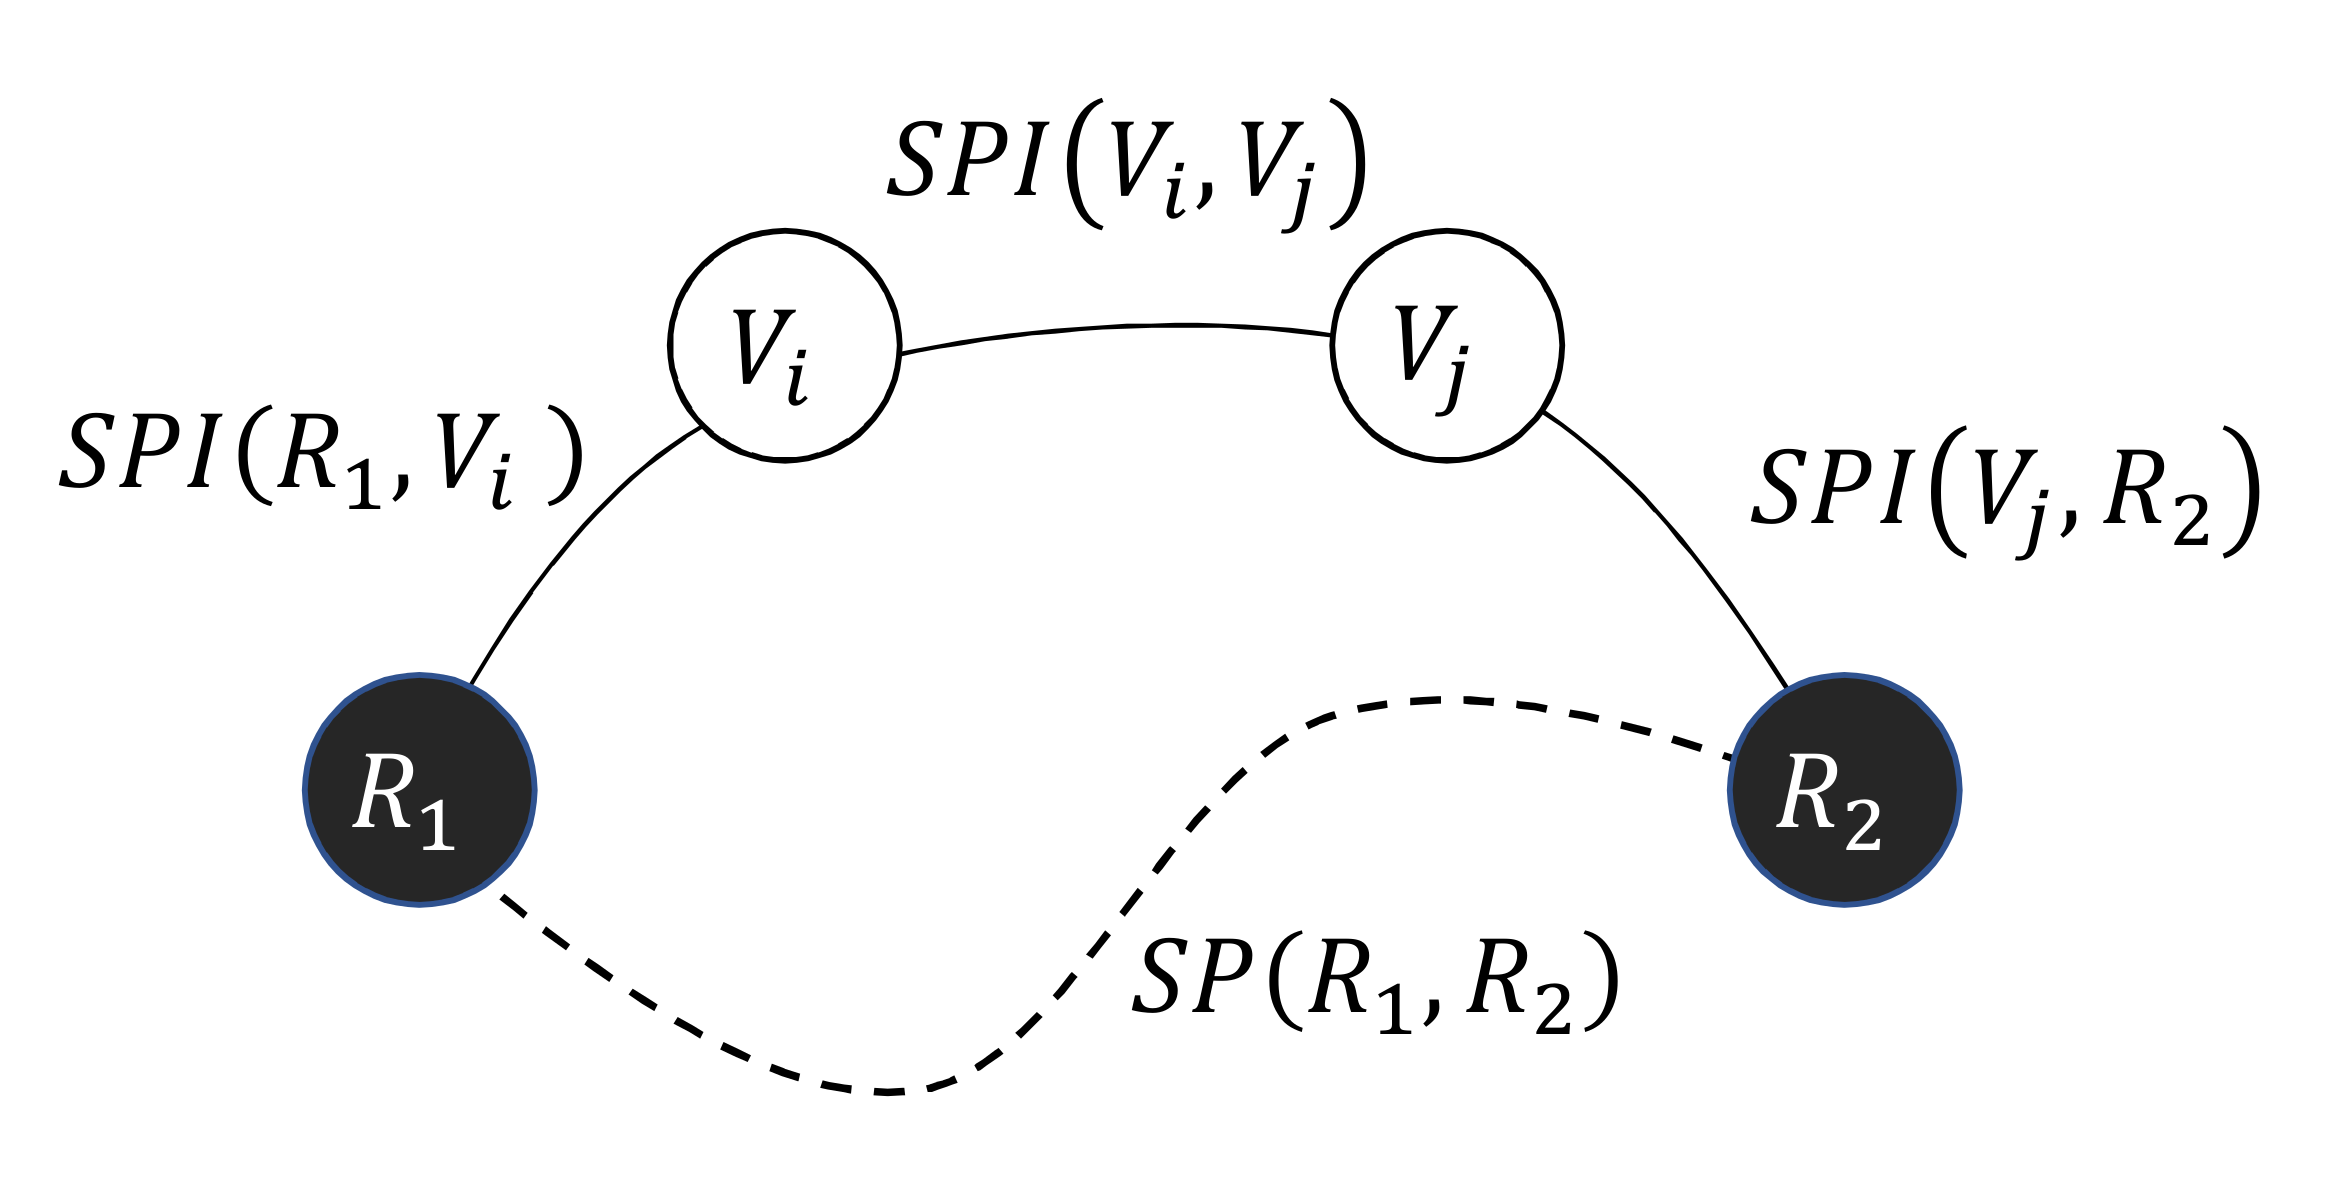
\includegraphics[height=1.5in]{figures/ShortestPathOnASingleSegment.png}
  \caption{Shortest Path On A Single Segment-Line} 
  \label{fig:ShortestPathOnASingleSegment} %% label for entire figure 
\end{figure}

Case 1: $V_x$ is between $V_i$ and $V_j$. The length of the path $V_i-V_x-V_j$ must be equal to $SPI\left(V_i,V_j\right)$ or there must be duplicated vertices on the path.

Case 2: $V_x$ is between $R_1$ and $V_i$ or between $V_j$ and $R_2$. $V_i-V_j$ should not be a part of the path or $V_i-V_j$ could be the shortest path. Then the path $V_i-R_1-R_2-V_j$ must be a part of $V_i-V_x-V_j$ because $R_1$ and $R_2$ are entrances of the \textit{segment-line}.

Since an all-pairs \textit{SPI} has a complexity of $O\left(n\right)$ and the \textit{n} here is much smaller than the number of points on the entire map, the time-cost for SPI is ignorable comparing to the time-cost of the entire map all-pairs shortest path calculation.

\textit{Lemma 2}: We assume that there are two different line-segments 

\noindent ${LS}_i=\left\{R_{i1},G_{i1},G_{i2},\cdots,G_{in},R_{i2}\right\}$ and ${LS}_j=\left\{R_{j1},G_{j1},G_{j2},\cdots,G_{jm},R_{j2}\right\}$. We pick a vertex $V_i$ from $LS_i$ and a vertex $V_j$ from $LS_j$, then the shortest path between $V_i$ and $V_j$ is 

\begin{equation} \label{GrindEQ__VRShortestOutside} 
\begin{split}
SP\left(V_i,V_j\right)=min\{SP\left(V_i,R_{i1},R_{j1},V_j\right),SP\left(V_i,R_{i2},R_{j1},V_j\right), \\
SP\left(V_i,R_{i1},R_{j2},V_j\right),SP\left(V_i,R_{i2},R_{j2},V_j\right)\}
\end{split}
\end{equation}

where ${SP}\left(V_i,R_{ia},R_{jb},V_j\right)={SP}\left(V_i,R_{ia}\right)+{SP}\left(R_{ia},R_{jb}\right)+{SP}\left(R_{jb},V_j\right)$. Here $V_i$ and $R_{ia}$ are in the same line-segment, so we can use Lemma 1 to calculate ${SP}\left(V_i,R_{ia}\right)$, so does ${SP}\left(R_{jb},V_j\right)$. The $SP\left(R_{ia},R_{jb}\right)$ is the only part we need to calculate using all-pair shortest path algorithms. We should notice that $R_{ia}$ and $R_{jb}$ could be the same vertex, but it does not make any difference to the lemma.

\textit{Proof}: Since $V_i$ and $V_j$ are not in the same \textit{segment-line}, there must be one or more reserved vertices on their shortest path. On $V_i$'s side, one of $R_{i1}$ and $R_{i2}$ must be on the shortest path. One of $R_{j1}$ and $R_{j2}$ should be on that shortest path, either. We assume that $R_{iu}$ and $R_{jv}$ are on the shortest path between $V_i$ and $V_j$, then a shortest path between $R_{iu}$ and $R_{jv}$ should be a part of that path.


\subsection{ Vertex Reduction}\label{subsecVR}

\noindent VRA iteratively removes ignorable vertices from the graph until only reserved vertices remain. In each iteration, we remove all ignorable vertices from the graph but keep the edges. If there are different routes between a pair of reserved vertices, we keep the shortest one and remove others. 


\subsubsection{ Remove Ignorable Vertices}\label{subsubsec_RIV}

\noindent Since the degree of ignorable vertices is no more than 2, an ignorable vertex has only 0, 1 or 2 neighbours. In the case of 0 or 1 neighbour, we simply delete the ignorable vertex; if it has two neighbours, we connect its two neighbours before it is removed, as shown in Figure \ref{fig:RemoveIgnorableVertices}. When we remove an ignorable vertex, the weight of the line which connects its two neighbours is equal to the sum of its recent two lines' weights (i.e., $W_l+W_r$). After we remove all ignorable vertices in a line-segment, the two reserved vertices at the end of the line-segment are connected with a line directly, whose weight is the sum of all the intermediate ones' (i.e., $W_1+W_2+W_3+W_4$).

\begin{figure} [hbtp]
  \centering 
  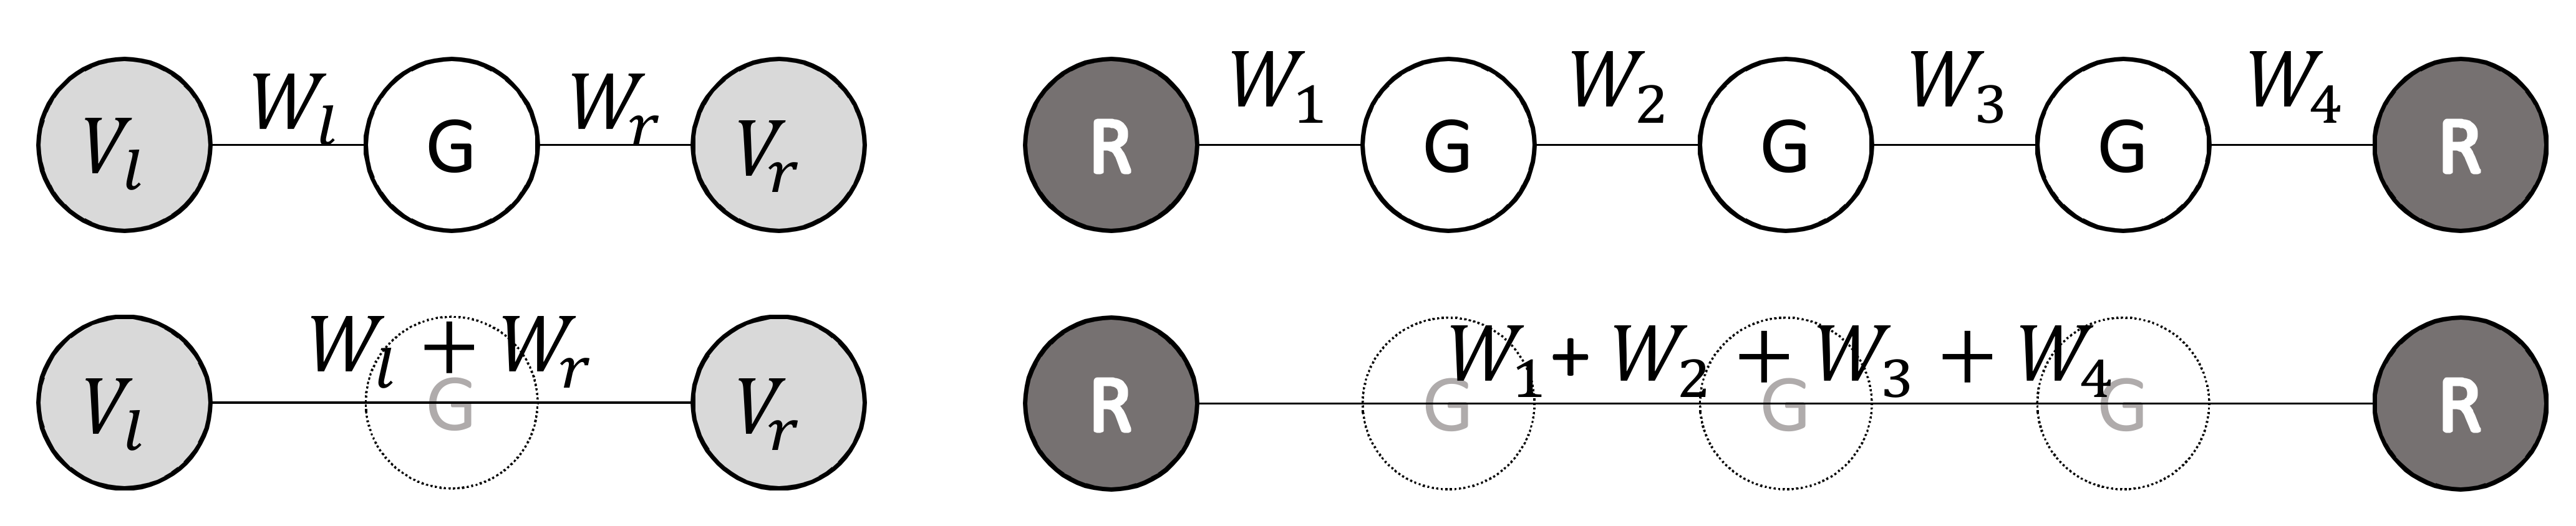
\includegraphics[height=1.2in]{figures/F51RemoveIgnorableVertices.png}
  \caption{Remove Ignorable Vertices} 
  \label{fig:RemoveIgnorableVertices} %% label for entire figure 
\end{figure}

\subsubsection{ Remove Redundant Connections}\label{subsubsec_RRC}

\noindent After we remove all ignorable vertices, all the reserved vertices are connected directly. However, it is possible that there are several connections between a pair of reserved vertices. Since the shortest route between a pair of neighbouring vertices makes other longer ones redundant, we remove all routes except the shortest one, as shown in Figure \ref{fig:F52TidyReservedConnections}. We assume that $W_2$ is the shortest line among three connections, when $W_1$ and $W_3$ are removed.

\begin{figure} [hbtp]
  \centering 
  
\includegraphics[height=1.2in]{figures/F52TidyReservedConnections.png}
  \caption{Tidy Reserved Connections} 
  \label{fig:F52TidyReservedConnections} %% label for entire figure 
\end{figure}

\subsubsection{ Iterations}

The process is shown in Algorithm \ref{AlgVerRed}. The input of the algorithm is the original entire map, which is called ${Graph}_0$. In the \textit{i}${}^{th}$ iteration, VRA makes a copy of ${Graph}_i$ as ${Graph}_{i+1}$. If $i>0$, the ${Graph}_i$ is the output of the previous (i.e., ${\left(i-1\right)}^{th}$) iteration. VRA removes all ignorable vertices in the ${Graph}_{i+1}$ as described in Section \ref{subsubsec_RIV} and remove all unnecessary routes between reserved vertices as described in Section \ref{subsubsec_RRC}. In other words, ${Graph}_i$ gets smaller and smaller as \textit{i} increases, because we always remove ignorable vertices from them. If ${Graph}_i$ is equal to ${Graph}_{i+1}$, which means that the \textit{i}${}^{th}$ iteration makes no modification on the graph, the algorithm ends.

\begin{algorithm} [hbtp]
\caption{Algorithm For Vertex Reduction}\label{AlgVerRed}
\begin{algorithmic}[1]
\Procedure {reduce} {${Graph}_i$}
\State Copy ${Graph}_i$ to ${Graph}_{i+1}$
\For {every ignorable vertex $G_u$ in ${Graph}_{i+1}$}
	\State $remove(G_u)$
\EndFor
\For {every pair of reserved vertices}
	\State remove redundant connections
\EndFor
\EndProcedure
\Procedure {VRA} {${Graph}_0$}
\State $i=0$
\While {$i=0$ or there is any difference between ${Graph}_{i-1}$ and ${Graph}_i$}
	\State $reduce({Graph}_i)$
	\State $i=i+1$
\EndWhile
\EndProcedure
\end{algorithmic}
\end{algorithm}

\subsection{ Assembling Vertices}\label{subsecAssVer}

\noindent We assume that the vertex reduction process stops at the \textit{i}${}^{th}$ iteration. Then, the ${Graph}_i$ is the input of an all-pairs shortest path algorithm. Let $SP_i\left(R_u,R_v\right)$ denote the shortest path from $R_u$ to $R_v$ in $Graph_i$. We can infer the all-pairs shortest path of ${\mathrm{Grap}h}_{i-1}$ based on ${\mathrm{Grap}h}_i$ with Lemma 1 and Lemma 2. The algorithm ends when we get the result of ${Graph}_0$. The algorithm is shown in Algorithm \ref{AlgAssIgnVer}.

\begin{algorithm} [hbtp]
\caption{Algorithm for Assembling Ignorable Vertices}\label{AlgAssIgnVer}
\begin{algorithmic}[1]
\Procedure {assemble} {${Graph}_i$}
\For {all ignorable vertices ($G_u$) in ${Graph}_i$}
	\For {all other vertices ($G_v$) in ${Graph}_i$}
		\If {$G_u$ and $G_v$ are in the same line-segment}
			\State Use Lemma 1 to calculate their shortest path.
		\Else
			\State Use Lemma 2 to calculate their shortest path.
		\EndIf
	\EndFor
\EndFor
\EndProcedure
\Procedure {AssembleAll} {$i$}
\While {$i>0$}
	\State $assemble\left({Graph}_{i-1}\right)$
	\State $i=i-1$
\EndWhile
\EndProcedure
\end{algorithmic}
\end{algorithm}

\noindent We start from the ${Graph}_{i-1}$ and assemble all intermediate graphs, until we get the result of ${Graph}_0$. For any intermediate ${Graph}_j$, we already have the all-pairs shortest path result of its reserved vertices in the previous iteration (i.e., ${Graph}_{j+1}$). Then, we calculate the shortest path from any ignorable vertex to all others. When the two vertices are in the same line-segment, we use Lemma 1 to calculate their shortest path. The Lemma 1 includes four parts: $SPI\left(V_i,V_j\right)$, $SPI\left(R_1,V_i\right)$, $SPI\left(V_j,R_2\right)$ and $SP\left(R_1,R_2\right)$. Since we already have the result of $SP\left(R_1,R_2\right)$ in the previous iteration, we just need to calculate the remaining three $SPI$ parts, which is easy and has fewer nodes. If the two vertices are in different line-segments, we use Lemma 2 to calculate the shortest path. We already have all the $SP$ parts from the previous iteration, so we just need to deal with their respective $SPI$ parts.


\section{ Finding Nodes in a Range}

\noindent We assume that there are $n$ nodes in a planar map (size: $h\times w$). Those nodes keep moving on the map slower than a speed threshold ($S$). If the distance between two nodes $a$ and $b$ is smaller than $r$, they are considered connected. We want to calculate all-pairs connections for all nodes on the map periodically. 

If we calculate these connections directly, the complexity is $\mathrm{O}\left(\frac{n^2}{2}\right)$. We assume that $r\ll min\left\{h,w\right\}$, and nodes are distributed on the entire map symmetrically. Then, the expected number of nodes which has a connection with a node ($v$) is $\frac{n}{h\times w}\times\pi r^2\ll n$. If we traverse all other ($n-1$) nodes of $v$, it will be a waste of time.

We propose an algorithm to optimize the calculation of all-pairs connections. We draw grids whose size is $l\times l$ on the map. When we calculate connections of the node $v$, only nodes in surrounding grids will be traversed.


\subsection{ Static Nodes}

\noindent If nodes on the map are stationary, the $r$ is the only factor of the selection of the grid size ($l\times l$). The length $l$ of the side of a grid should be equal to $r$, as shown in Figure \ref{fig:F53GridSizeForStillNodes}. For any node $v$ in the dark grid, all nodes whose distance between them is equal to or shorter than $r$ should be in the grey or dark grid. Therefore, if we want to get all connected nodes to node $v$, we simply need to traverse all nodes in the grey and dark grids instead of all nodes in the entire map. In this case, the expected number of nodes which we need to traverse is $\frac{9n\times r^2}{h\times w}$ for checking connections for a node $v$. If we calculate connections for all nodes, we simply need to get the distances of about $\frac{9n^2\times r^2}{2\times h\times w}$ pairs of nodes, instead of $\frac{n^2}{2}$ pairs.

\begin{figure} [hbtp]
  \centering 
  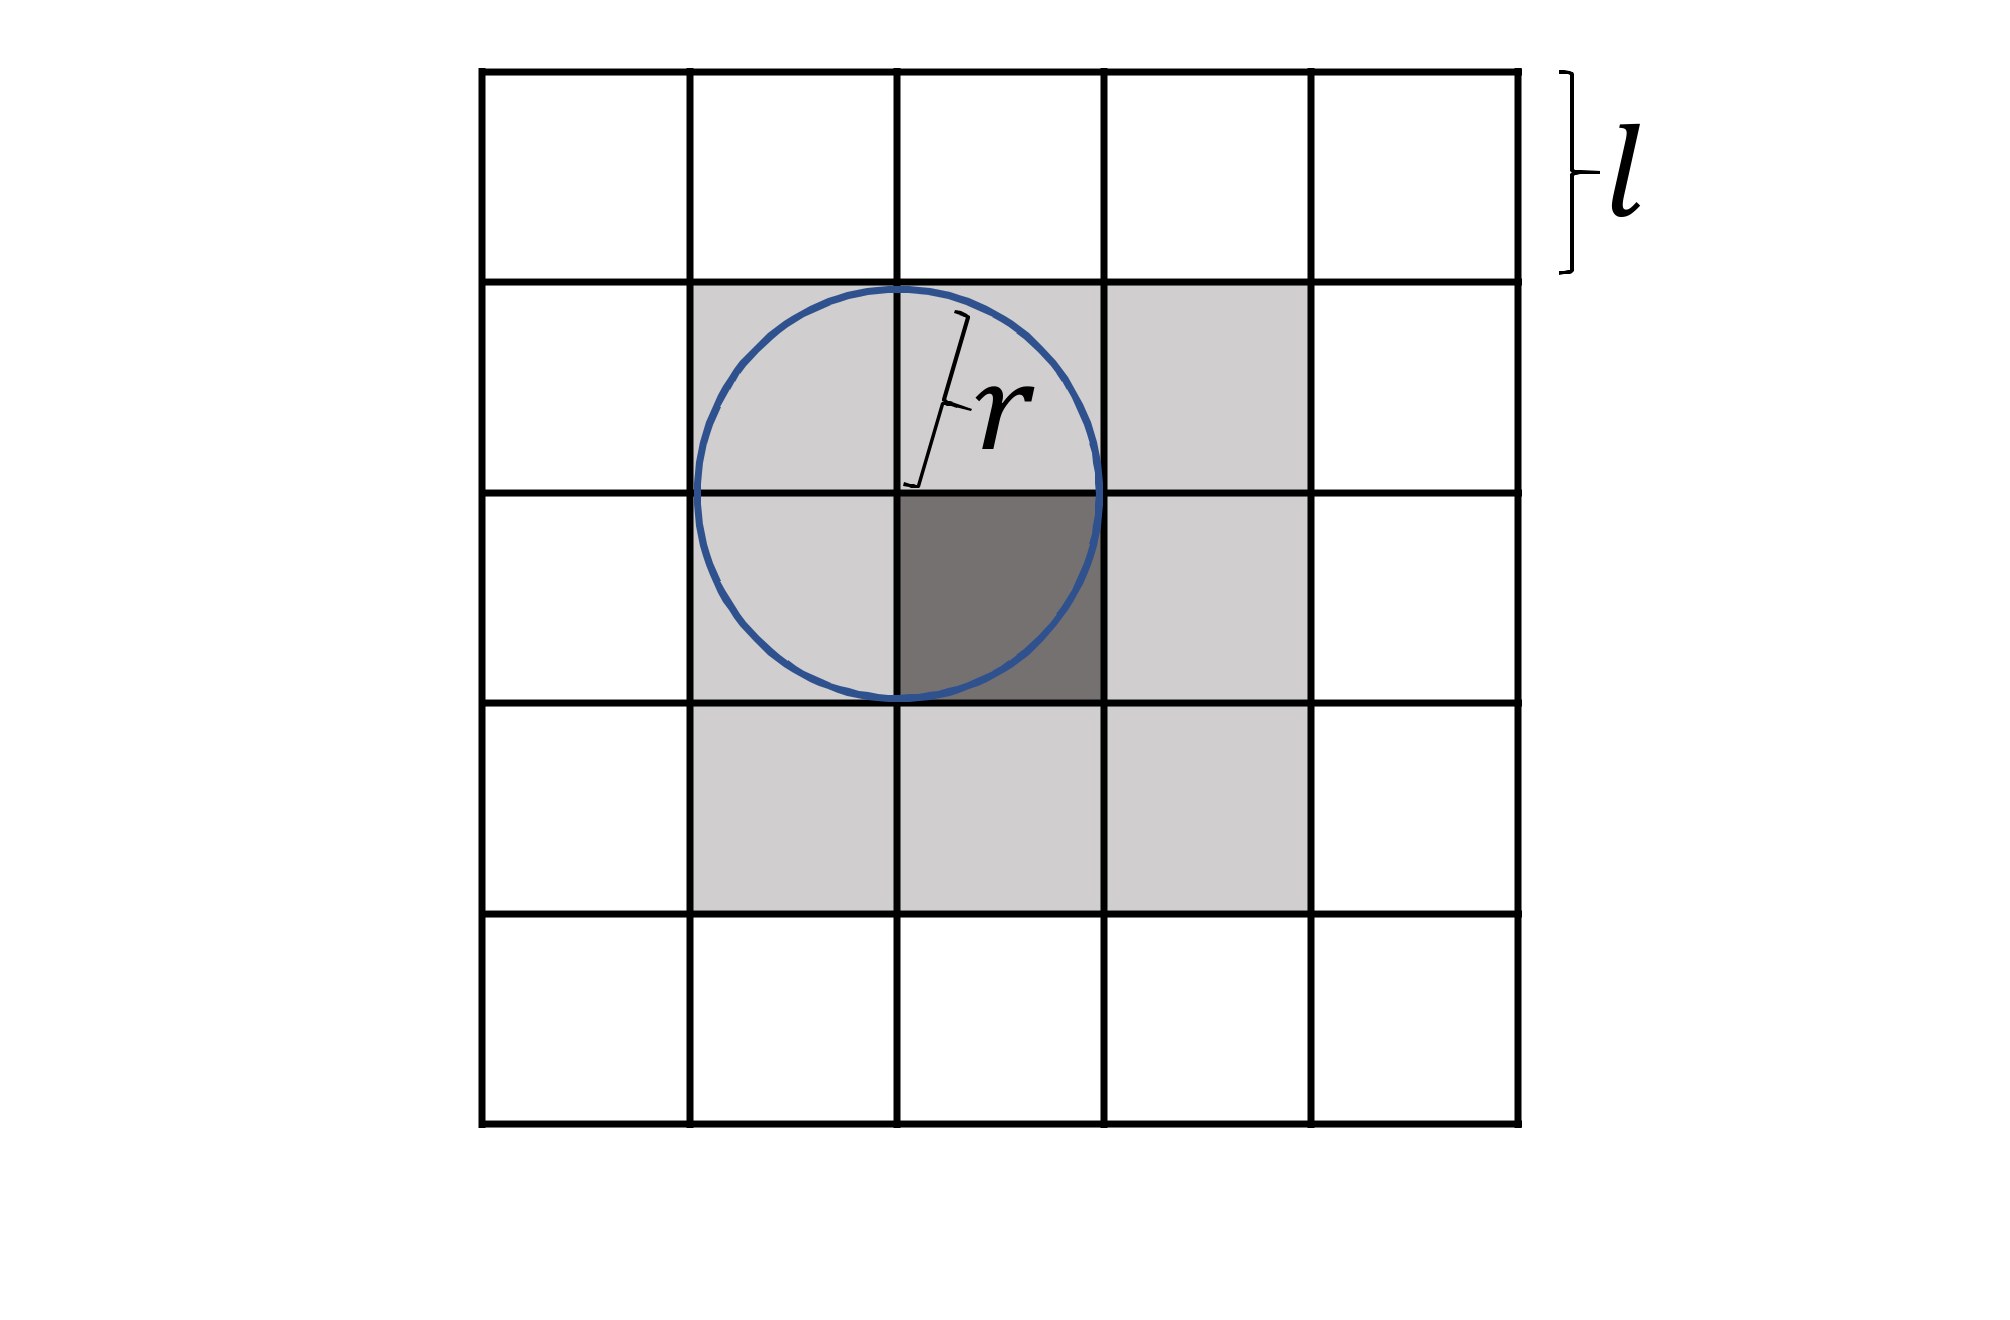
\includegraphics[height=2in]{figures/F53GridSizeForStillNodes.png}
  \caption{Grid Size For Still Nodes} 
  \label{fig:F53GridSizeForStillNodes} %% label for entire figure 
\end{figure}


\subsection{ Mobile Nodes}

\noindent The problem is a bit more complicated if nodes are moving. Assuming that we want to calculate all-pairs connections at $t_1$, first, we draw grids at time $t_0$, so that we know which grid is a node in at $t_0$. Instead of $t_0$, we want to get connections at $t_1$. In this case, the length $l$ should be larger than $r$.

Suppose that we have two nodes $u$ and $v$, and their distance is $d_1$ at $t_1$. Since the maximum speed of nodes is $S$, their distance $d_0$ at $t_0$ satisfies
\[max\left\{0,d_1-2\delta \right\}\le d_0\le d_1+2\delta \] 
where $\delta =S\left|t_1-t_0\right|$. When $d_1\le r$, these two nodes are connected at $t_1$, then $d_0$ must satisfy $0\le d_0\le r+2\delta $. As shown in Figure \ref{fig:F54LengthofGrid}, If we draw grids on the map in an attempt to place the two nodes in the same or adjacent grids at $t_0$, the length of each grid $l=r+2\delta $.

\begin{figure} [hbtp]
  \centering 
  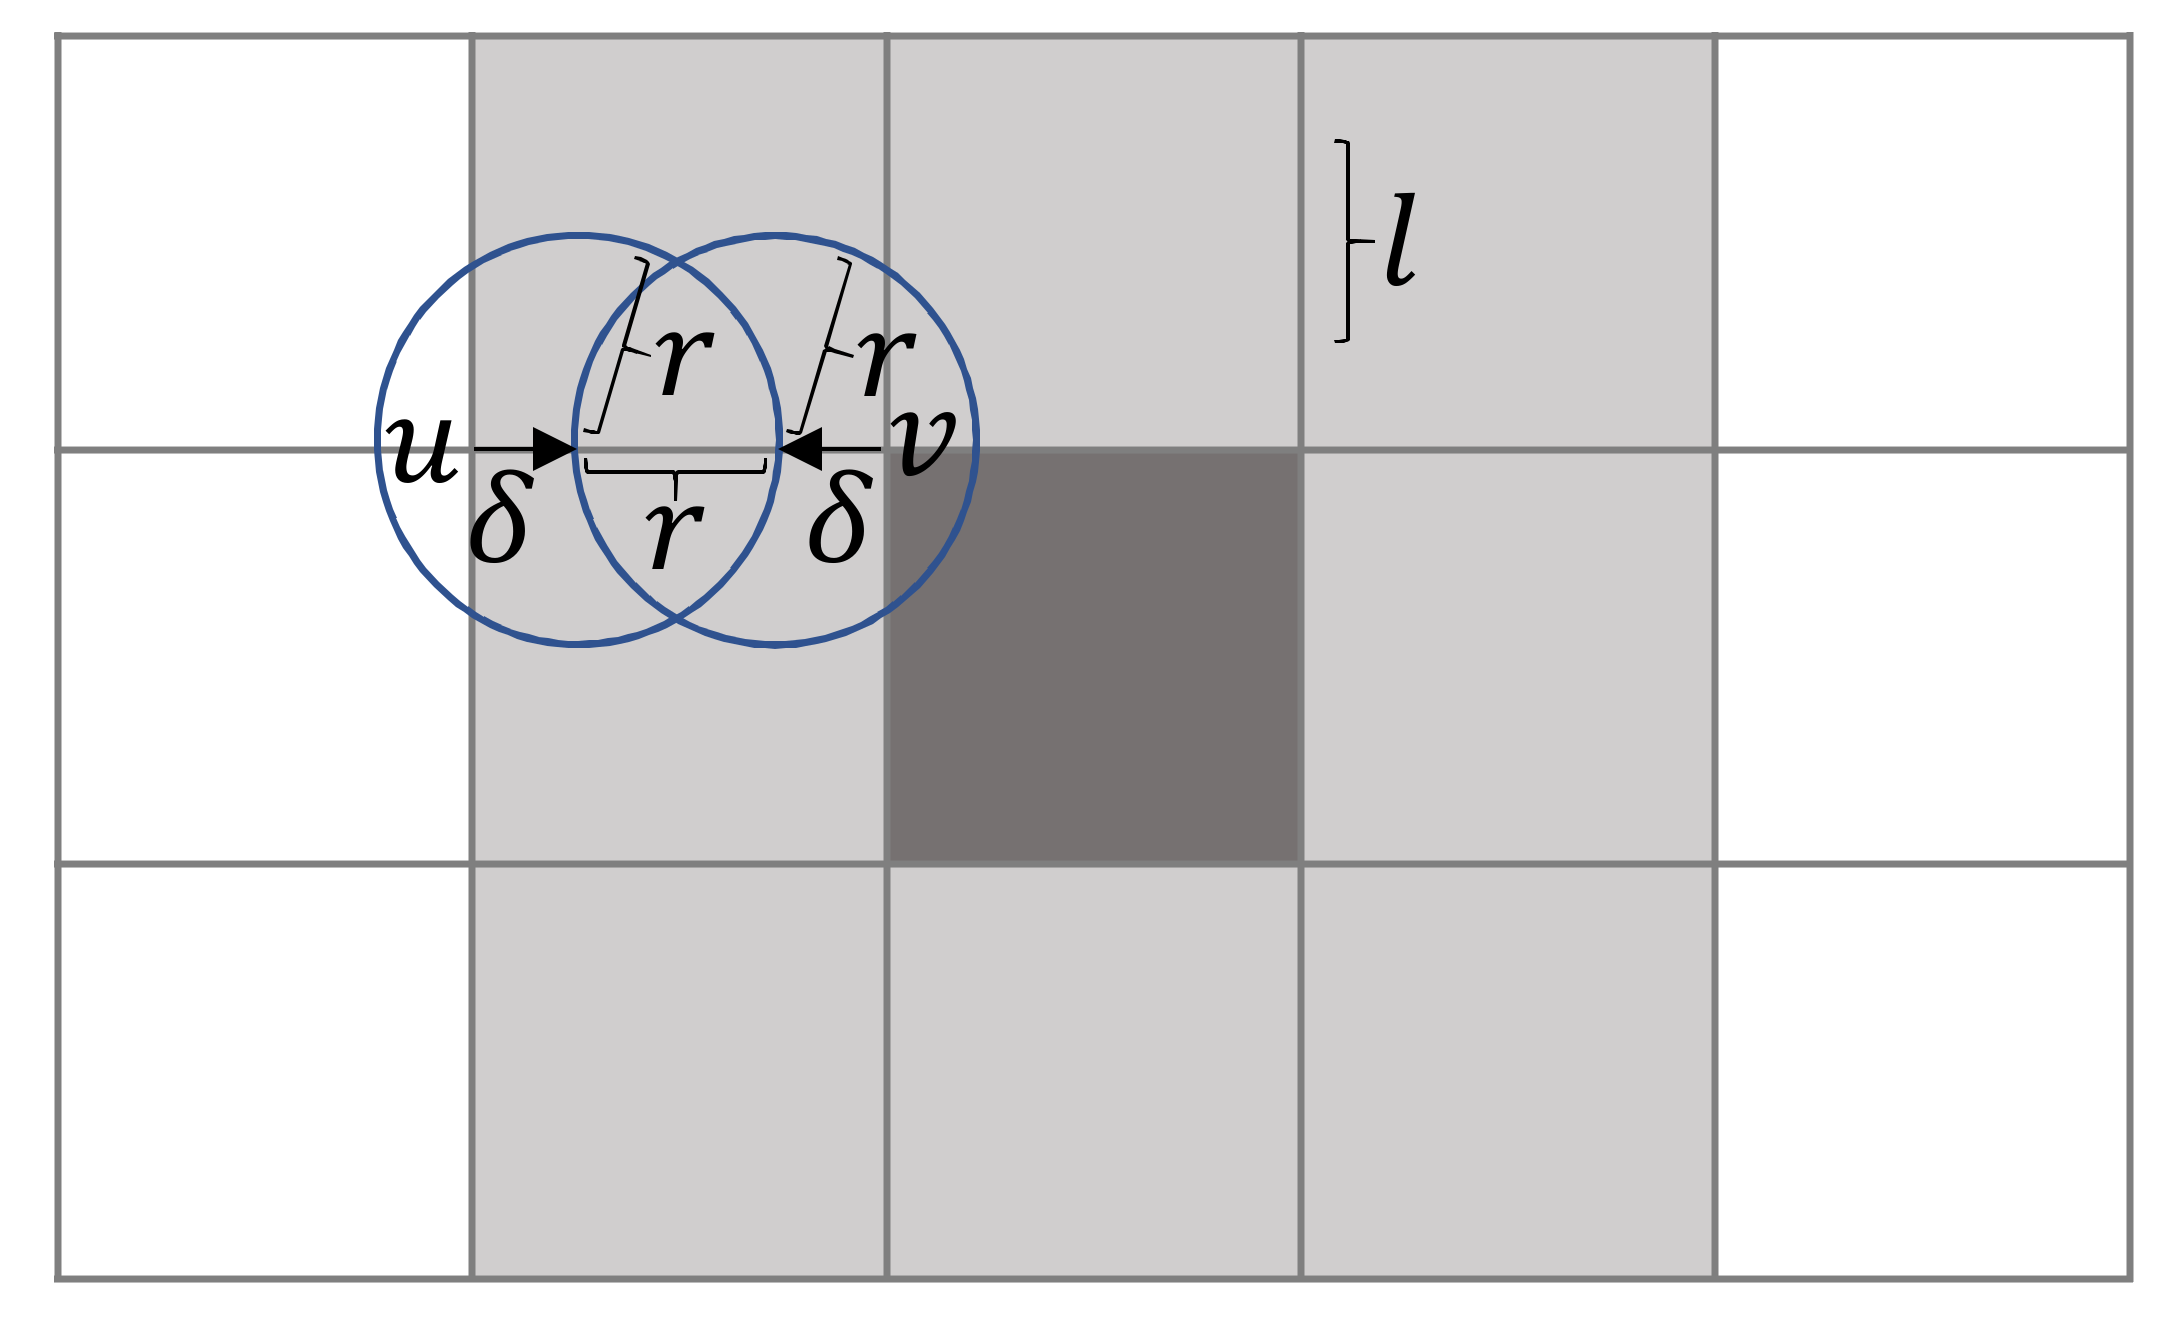
\includegraphics[height=2in]{figures/F54LengthofGrid.png}
  \caption{Length of Grid} 
  \label{fig:F54LengthofGrid} %% label for entire figure 
\end{figure}

\subsection{Complexity}

\noindent The complexity of drawing grids is $\mathrm{O}\left(n\right)$, while that of checking connections is $\mathrm{O}\left(\frac{9n^2\times l^2}{2\times h\times w}\right)$, so the checking part is much more expensive than the drawing part. Since $l=r+2\delta =r+2S\left|t_1-t_0\right|$, the checking part achieves its best performance when $t_1-t_0=0$, then its complexity is $O\left(\frac{9n^2\times r^2}{2\times h\times w}\right)$. That is equal to the complexity when nodes are stationary.




















%%%%%%%%%%%%%%%%%%%%%%%%%%%
\chapter{ Conclusion and Future Work}
\label{CFW}
%%%%%%%%%%%%%%%%%%%%%%%%%%%
 

\noindent In this chapter, we will summarize our findings and discuss the future directions of the proposed work in the previous chapters yet to be explored. 


\section{ Summary of Work Done}

\noindent In this thesis, we proposed and analyzed two new location-privacy preserving protocols, namely MSLPP and ACP, besides developing a new OMSN simulator, called ORS, as a platform for evaluating the proposed protocols and comparing them with their counterparts.

Our first protocol, MSLPP, is a distributed location-privacy preserving protocol using social-relationship and encryption. Simulation results show that it has a better performance on delivery success ratio and provides an acceptable obfuscation compared to its counterpart HSLPO which is an improvement of their earlier scheme SLPD. Compared to HSLPO, our scheme MHLPP achieves an in increase in success ratio between 6\% and 11\% for the same range of parameters considered by the authors of SLPD. The success ratios of both HSLPO and MHLPP decline when the privacy threshold is increased, while the success ratio of HSLPO is always lower than that of MHLPP and decreases more sharply than that of MHLPP. Although HSLPO is slightly more secure than MHLPP based on our experiments which means the original requester has a lower rate to be located, but the entropy difference is quite small and negligible. Encryption and decryption to enhance security are added cost for MHLPP which is acceptable. Our experiment (using the map of Helsinki) presents that in a social network with 126 users, the average number of times of a query is encrypted and decrypted is less than 3 when the privacy threshold is considered as 85.

Our second proposed Appointment Card Protocol ACP also uses social relationship for preserving location privacy. It facilitates the obfuscation process by continuously exchanging appointment cards among users so that the original requester does not communicate with any of his friends when initiating a query. Simulation results show that it has a better performance with respect to the query-delivery success ratio and provides an acceptable obfuscation compared to its counterparts. Although ACP requires slightly more time to forward the reply, the total time required for query delivery and reply delivery is still less than that for its counterparts SLPD and MHLPP. The major disadvantage is that the ACP must exchange ACs continuously, which can consume network resources. However, that cost is low if users do not send too many queries.

\noindent To facilitate our experimentation, we have developed a simulator, called ORS, which is more suitable for OMSN simulation than the existing simulator, ONE. The ORS is more reliable and efficient than ONE for simulating opportunistic social networks. 


\section{ Future Work}

\noindent In MHLPP, we just considered the relationship strength between two connected people in the social network; in other words, an agent only gives the message to his direct friend. In most of the cases, the friends of your friends can also be trusted and be considered. If these friends can participate in forwarding queries, agents can have more choice in the obfuscation phase.

In ACP, the sizes of agents' relay tables are significantly affected by the number of appointment cards passing by them. If we can decrease the number of appointment cards in the network, the burden of agents can also decline. For example, a single appointment card can be shared among friends instead of being used by only one user.
%%%%%%%%%%%%%%%%%%%%%%%%%%%%
\chapter {General Chordal Rings}
\label{GL}
%%%%%%%%%%%%%%%%%%%%%%%%%%%
Now that we have investigated the problem of disinfecting a network from a  \bv   in   special  classes of chordal rings, we will discuss the problem in general chordal rings, regardless of chords structure.  


The solution  we propose is based on the  idea described for the general chordal ring in Chapter \ref{PM}, and has already been explained throughout this thesis. It involves an exploring phase, followed by a surrounding phase. Our protocol is based on a general surrounding method that can be applied to any chordal ring structure, regardless of the number or distance of chords. It must be noted that the move-cost for this method is not optimal.

 


 \section{Exploring and Shadowing}
%The main goal of this phase is to determine the location of the original \bv since the location of the \bv is unknown a priori. This process is done by the  exploring team: $LEA$,$EA$, and shadow agent(s) $SA$. 
%Finding the node in which the \bv resides implies creating more \bvs in some cases, destroying $EA$, and clearing that node. As we mentioned before, the technique used in this phase is the {\em safe exploration}.
%\begin{comment}
%Starting from a random node, \hb, $v_0$, the leader and the exploration agent explore the chordal ring
%node by node along the outer ring  (i.e., using only $d_1=1$) in the clockwise direction.  $EA$ moves to the next node $v_{1}$ while $LEA$ waits at $v_{0}$; if $EA$ returns back to its leader, then $v_{1}$ is not a \bv and they both move to $v_{1}$ and so on. However, if $LEA$ receives a \bv instead of $EA$, then the location of the original \bv is detected. 
%\end{comment}
%In order maintain monotonicity, $SH$s are deployed. The deployment of $SH$s starts when $LEA$ and $EA$ have explored at least $d_2$ nodes. 
%\begin{comment}
%In other words, if  $C_n( d_1=1, d_{2}, ..., d_{m})$, and the exploring team currently exploring node $v_j$
%and $\left\vert{S_{area}}\right\vert \ge d_2$, at least one $SA$ is deployed and the number of $SA$s increases as many as the neighbours of the current explored node in the safe area, the number of $SH$s $=|N_{ex}(v_j)|-1$.
%Once $EA$ arrives to the \bv location, it is destroyed, $LEA$ receives a $BV$ instead of EA, that node is cleared, new \bvs are located at all the unprotected(unexplored) neighbours of the original $BV$.
%
%  Since we have a monotone protocol, the explored nodes  in ($S_{area}$) should be protected from potential recontamination. As we mentioned before, the exploring team ($LEA$,$EA$) are moving in clockwise direction along the outer ring, but when they reach a certain node ($v_{n-d_m}$), the possibility of infecting explored node(s) increases; thus, in addition to $SH$s at counter clockwise neighbours, $SH$s are needed at the clockwise neighbours . As we have mentioned before, the area in which the recontamination possibility increases is called danger area  $D_{area}$ where $v_{n-d_m} \leq D_{area}\leq v_{n-1} $.
%\end{comment}
% 
%
%  \begin{center}
%\fbox{
%\begin{minipage}{6 cm}
%{\sc  Exploring and Shadowing}
%  \begin{tabbing}
%  Age\= nts $EA $ and $$LEA$$ at safe node  $v_i$.\\
%\\
% - Compute  $N_{ex}(v_{i+1})$ \\
% - For each $q \in N_{ex}(v_{i+1})$ \\
% \tab  $SH$\ is deployed \\
% - $EA$ moves to $v_{i+1}$\\ \\
% If $EA$ returns back to $v_{i}$\\
% \tab $LEA$ and $EA$ move to $v_{i+1}$\\
% Else (i.e., $BV$ moves to $v_{i}$)\\
%\tab $EA$ is destroyed\\
% \tab $|BV|=N_{un}(v_i)$
%  \end{tabbing}
%\end{minipage}
%}
%\end{center}
%

 The   phase is  described in detail in Chapter \ref{PM}. The following are our observations in general chordal ring structures:

\begin{theorem}

In any  chordal ring $C_n=\{1,d_2,d_3,...,d_m\}$, in the worst case scenario, the \bv is detected in $((2+m)n-2m-3)$ moves.

\end{theorem}
\begin{proof}
The worst case scenario regarding the number of moves required occurs when the \bv  is located at node ($v_{n-1}$) after exploring   $n-1$ nodes.  
 The complexity of this case would be $3n-5$ for the movement of $LEA$ and $EA$, $(\sum\limits_{i=2}^m n-1-d_i)$ for the movement of $SH$s to counter-clockwise neighbours and $(\sum\limits_{i=2}^m d_i-1)$ for $SH$s to clockwise neighbours. 

 In this case, the \bv triggers no new \bvs since all of the neighbouring nodes are occupied by $SH$s, ($2m-1$) $SH$s. This case is considered the worst case scenario in terms of calculating the number of moves, but the best case in terms of cleaning and surrounding agents.
\end{proof}

 
\begin{theorem}

In any  chordal ring $C_n=\{1,d_2,d_3,...,d_m\}$, the worst case scenario regarding the number of agents required for disinfection would occur when $2m-1$ new \bvs are created after triggering the original virus.
\end{theorem}
\begin{proof}
If the \bv is found at node $(v_i)$ where $1\leq v_i< d_2$, the spread of \bvs would be maximized since no $SH$s have been deployed and the explored neighbours $|N_{ex}(v_i)|=1$, which is $v_{i-1}$ and  is occupied by the  $LEA$. Therefore , the number of unexplored neighbours, o \bvs, is $2m-1$. This number of \bvs requires a high number of surrounding agents. 
\end{proof}



As usual, this phase comes to an end when the \bv is detected and triggered. At this point, new \bvs have been created and moved to the unexplored neighbouring nodes. It is at this point that the second phase begins. 



\section{Surrounding and Eliminating}
 
As described in Chapter \ref{PM}, once the \bv node is detected, the $LEA$ moves to its location and the {\em Surrounding and Eliminating} phase begins.
%
%  \begin{center}
%\fbox{
%\begin{minipage}{7.5cm}
%{\sc Surrounding and Eliminating} 
%  \begin{tabbing}
% $$LEA$$ \= and  $SH$s  covering all $N_{ex}(v)$ \\
% $BV$ comes back from $v$. \\
%  \\
%\>-$SH$s make one move in the clockwise direction.\\
%  \> - Compute  $N_{un}(v)$\\
% \> - For \= each $u \in   N_{un}(v)$:\\
% \>\> Deploy  an  agent  to each  $z\in \{N(u)\setminus  N_{un}(v)\}$\\
% \>\> Wh\=en $N(u)$ is covered:\\
% \>\>\> Deploy one agent to   $u$
%  \end{tabbing}
%\end{minipage}
%}
%\end{center}
%
%

Throughout our study of different classes of chordal rings, we have proposed two routing variations: local and non-local strategies. We have seen in previous chapters that these strategies work for some topologies and not others. For example, the local greedy approach causes correct routing in double loop chordal rings and infinite loops in triple loop and consecutive-chords rings. We can thus deduce that the simple greedy would not work in general chordal rings with arbitrary chord structures (see \ref{no-greedy}). The non-local move-optimal strategy would always work for any chordal rings since this approach requires precise information about the chord structure which is available to the $LEA$ and complex  to calculate. We have observed the following from both strategies:

\begin{itemize}
\item  If node $x_{0}$ represents the location of the original \bv, node $x_{-1}$ is always safe because it is occupied by an agent. This means that it can be used as a starting point to reach any target.
\item After triggering the original {\it black virus}, the new \bvs divide the outer ring into enclosed and open segments. Enclosed segments are areas that include the following set of nodes: $\{ x_{\pm d_i-1}, x_{\pm d_i-2}, x_{\pm d_i-3},..., x_{\pm d_{i\pm1}+1}\}$. Open segments are areas that include the following set of nodes: $\{ x_{\pm d_m\pm1},  x_{\pm d_m\pm2}..., x_{\pm d_m}\}$.
\item Once the agents reach node $x_{\pm d_i-1}$, they are able to reach close targets greedily. In order to avoid getting stuck in infinite loops, agents can reach their close targets by using the one-direction greedy approach. 
\end{itemize} 

%clockwise neighboursEA={ x_{ d_i-1}, x_{d_i-2}, x_{ d_i-3},..., x_{ d_{i-1}+1}}
%counter clockwise neighboursEA={ x_{ -d_i-1}, x_{-d_i-2}, x_{ d_i-3},..., x_{ -d_{i+1}+1}}
Making use of the observations above, we propose an efficient general strategy that is capable of disinfecting any chordal ring and gives upper bounds for the optimal paths.
In this approach, all targets are reached through node $x_{-1}$. The set of targets is calculated based on the location of the original $BV$ and the agents are scattered between $BV$s. The topology is thus divided into {\it enclosed areas} and {\it open areas}.



Note that with respect to node $x_{-1}$, some targets are in the clockwise direction while others are in the counter-clockwise direction.

In order to reach the targets, the $LEA$ deploys agents through $x_{-1}$. The agents then move to the closest neighbour that is greater than or equal to its destination. Once the agent reaches $x_{\pm d_i-1}$, it arrives to the area in which its target resides. The agent then moves greedily in one direction until it reaches its destination. Since this is a one-direction greedy approach, the agent only moves to neighbouring nodes that are greater or equal  to its target. Only in one case an agent moves to a neighbour that is smaller than its target, when $t=x_{2d_m}$. Figure \ref{fig:general_algo} shows an example of this strategy.
\begin{figure}[H]
  \centering  
  \includegraphics[width=0.5\textwidth]{figures/general_algo.jpg}
  \caption{ The paths to reach some targets using the general strategy.}\label{fig:general_algo}
\end{figure}


\begin{comment}

  \begin{figure}[h]
\centering
\includegraphics[scale=0.60]{example.pdf}
\caption{Chordal ring C(1,4,11,13,17)}
\label{fig:example}
\end{figure}

\end{comment}
 







\begin{center}
\fbox{
\begin{minipage}{7.5 cm}
{\sc General Deployment Strategy}
\begin{tabbing}
Depl\=oying agent $A$ arriving at $x_j$ from $y$ with destination $t$\\ 

If $t =x_{z}$ where $z \in \mathbb{Z}^+ $\\
\tab if  $j=0$\\
 \tab \tab move to $ x_{-1} $ \\ 
\tab if  $j=-1$ \\ 
\tab\tab move to $ x_{d_{i}-1} $ such that  $x_{d_{i}-1} \ge t$ , and $x_{d_{i}-1} $ minimizes $dist(x_{-1},t)$ \\ 
\tab Else\\
\tab\tab if  $t > x_{d_m}$\\
\tab\tab\tab move to $x_{d_m-1}$ then to $x_{2d_{m}-1}$ (i.e., move to the open area)  \\
\tab\tab\tab If $t=x_{2d_{m}}$\\
\tab\tab\tab\tab move to $x_{2d_{m}}$\\
\tab\tab\tab Else\\
\tab\tab\tab compute $next$\\
\tab\tab\tab\tab let $OA=\{ x_{2d_{m}-1},x_{2d_{m}-2},...,x_{d_{m}+1}\}$the open area set \\
\tab\tab\tab\tab  Let $FD =\{ N(x_j)- y- BV \}$ be the set of feasible destinations.\\
\tab\tab\tab\tab let $C=FD  \cap OA$ \\
\tab\tab \tab\tab Agent $A$ moves to $next \in C$ that minimizes $dist(x_j,t)$ and $next \ge t$\\
\tab\tab Else\\
\tab\tab\tab compute $next$\\
\tab\tab\tab\tab let $EA=\{x_{d_i-2},x_{d_i-2}, x_{d_i-3},x_{d_i-4},...,x_{d_{i-1}+1}\}$the enclosed area set \\
\tab\tab\tab\tab  Let $FD =\{ N(x_j)- y - BV \}$ \\%be the set of feasible destinations.\\
\tab\tab\tab\tab let $C=FD  \cap EA$ \\
\tab\tab \tab\tab Agent $A$ moves to $next \in C$ that minimizes $dist(x_j,t)$ and $next \ge t$\\
\end{tabbing}
\end{minipage}
}
\end{center}


\begin{center}
\fbox{
\begin{minipage}{7.5 cm}
{\sc General Deployment Strategy}
\begin{tabbing}
Else (i.e.,  $t =x_{z}$ where $z \in \mathbb{Z}^- )$\\
\tab if  $j=0$\\
 \tab \tab move to $ x_{-1} $ \\ 
\tab if  $j=-1$ \\ 
\tab\tab move to $ x_{-d_{i}-1} $ such that  $x_{-d_{i}-1} \ge t$ , and $x_{-d_{i}-1} $ minimizes $dist(x_{-1},t)$  \\ % the closest large neighbour of x_{-1} to t
\tab Else\\
\tab\tab if  $t < x_{-d_m}$\\
\tab\tab\tab move to $x_{-d_m-1}$  (i.e., move to the open area)  \\
\tab\tab\tab compute $next$\\
\tab\tab\tab\tab let $OA=\{x_{-d_{m}-1}, x_{-d_{m}-2},x_{-d_{m}-3},...,x_{-2d_{m}}\}$the open area set \\
\tab\tab\tab\tab  Let $FD =\{ N(x_j)- y- BV \}$ \\%be the set of feasible destinations.\\
\tab\tab\tab\tab let $C=FD  \cap OA$ \\
\tab\tab \tab\tab Agent $A$ moves to $next \in C$ that minimizes $dist(x_j,t)$ and $next \ge t$\\
\tab\tab Else\\
\tab\tab\tab compute $next$\\
\tab\tab\tab\tab let $EA=\{x_{-d_i-1},x_{-d_i-2}, x_{-d_i-3},x_{-d_i-4},...,x_{-d_{i+1}+1}\}$the enclosed area set\\
\tab\tab\tab\tab  Let $FD =\{ N(x_j)- y - BV \}$ \\%be the set of feasible destinations.\\
\tab\tab\tab\tab let $C=FD  \cap EA$ \\
\tab\tab \tab\tab Agent $A$ moves to $next \in C$ that minimizes $dist(x_j,t)$ and $next \ge t$\\
\end{tabbing}
\end{minipage}
}
\end{center}






\noindent  The following observations were made after using the general strategy:

\begin{theorem}
In any chordal ring $C_(1,d_2,d_3,....d_m)$ with $d_m<<n$, the worst case scenario in terms of number of agents required occurs when triggering the original \bv creates $2m-1$ more {\it black viruses}. In this case,  $size(C)\leq  \lfloor \frac {4m^2-8m+3}{2} \rfloor +6m-1$ and $Spread(C)=2m$.
\end{theorem}

\begin{proof}


In any chordal ring $C$, the worst case scenario occurs when the original \bv is found before deploying any $SH$. In orther words, 
when $|S_{area}|<d_2$. In this case, the maximum number of \bvs would be created: $ 2m-1$ and $\cal BV$ $=\{x_{1}$, $x_{\pm d_2}$, $x_{\pm d_3}$, ..., $x_{\pm d_m}\}$. If we assume that the chords are well separated ( i.e., $d_i-d_{i-1}\ge1$), we have $2(m-1)$ enclosed areas and $2$ open areas.
Each $bv\in BV$ has at most $2m-1$ neighbours which represent our targets. Some of these are common neighbours or other \bvs, depending on the structure of  the chords. Because we are interested in calculating the $size(C)$, we must first find the number of targets. Each $bv \in BV$ has common neighbours and non-common neighbours. $N_{nc}(bv)$ and $N_{c}(bv)$ denote the set of non-common neighbours and the set of common neighbours of any $bv \in BV$. Note that for any $i$ and $j$, $x_{d_i}+x_{-d_j}$ (a neighbour of node $x_{d_i}$) is the same as $x_{-d_j}+x_{d_i}$ (a neighbour of node $x_{-d_j}$). We have thus found that $|N_{nc}(bv)|\leq2$ and $|N_{c}(bv)|\leq 2m-3$ for any $bv \in BV$. In other words, each \bv has a maximum of two non-common neighbours.  Therefore, we can calculate the maximum possible number of targets as: $|\cal T|$$\leq \lfloor \frac {4m^2-8m+3}{2} \rfloor +4m-2$. $|\cal T|$ represents the number of $SA$s we need to surround the \bvs in the system.
%|N_{nc}(bv)|=2(2m-1), and |N_{nc}(bv)|=((2m-1)(2m-3))/2 floor

The team of agents  consists of $\leq \lfloor \frac {4m^2-8m+3}{2} \rfloor +4m-2$ $SA$s, one $LEA$ and $(2m)$ $CA$s. Therefore $size(C)\leq  \lfloor \frac {4m^2-8m+3}{2} \rfloor +6m-1$ and $Spread(C)=2m$.

\end{proof}


\begin{theorem}

In any chordal ring  $C_(1,d_2,d_3,....d_m)$ where $\left\vert{S_{area}}\right\vert < x_{d_2}$,  the number of moves required to surround and eliminate $BV$s  is $O( {m^2} )$.
\end{theorem}

\begin{proof}
Calculating the number of moves is not trivial in the general case. This approach is not optimal but it is efficient and gets the routing done correctly. We have an upper bound for the total number of moves required and it is constant. In the analysis of our strategy we find:
\begin{itemize}

\item $2m-1$ targets are reached in $2$ moves, which are $N(x_{-1})$:
$$ x_{0}\xrightarrow {-1}x_{-1} \xrightarrow {\pm d_i} x_{\pm d_i-1}$$

\item Two targets are reached in $4$ moves each which are  $x_{2d_m}$ and $x_{-2d_m}$.
$$ x_{0}\xrightarrow {-1}x_{-1} \xrightarrow {\pm d_m} x_{\pm d_m-1} \xrightarrow {\pm d_m} x_{\pm 2d_m-1}\xrightarrow {\pm 1} x_{\pm 2d_m}$$

\item The rest of targets are nested in the enclosed and open areas and their locations are solely dependent on the chords structure. 
In order to reach them, the agents first move to  node $x_{-1}$ and then to one of the neighbours that satisfies the strategy's conditions. Once an agent is located at the beginning of an interval in which its destination resides, the one-direction greedy strategy begins. 

 The destination between $x_{\pm d_i}$ and $t$ can be minimized if there is a chord $d_i>1$. In our thesis we will consider the worst case scenario in which an agent moves to its target through $\pm 1$ chords. Therefore, each of the other targets, $\leq \lfloor \frac {4m^2-8m+3}{2} \rfloor +2m-3$, are reached in  $O( m^2)$ moves.
%$\leq \lfloor \frac {4m^2-8m+3}{2} \rfloor +4m-2  - (2m-1+2)$ (2m-1+2)is the number of the targets we %know exactly how to reach.
%$\cal T$$={t_1,t_2,...,t_j}$
%he  rest targets, $\leq \lfloor \frac {4m^2-8m+3}{2} \rfloor +2m-3$, is reached at most $dist(x_{\pm d_i-1},t_j)$ where $t_j\in$  $\cal T$. Summarizing, the number of moves would be
\end{itemize}
\end{proof}





%
%
%
%
%\subsection{Correctness and Complexity}
%
%For disinfecting any  chordal ring $C_n(d_1=1,d_2,d_3,\ldots d_m)$ with $d_m<<n$, from {\it black viruses}, we have an efficient general algorithm that consists of two phases: {\em Exploring and Shadowing} and {\em Surrounding and Eliminating}. 
%
%\begin{theorem}
%
%The  general algorithm  successfully disinfect any chordal ring from \bvs in a monotone synchronous way. 
%
%\end{theorem}
%
%\begin{proof}
%The correctness of the first phase follows from the fact that the exploring team explores nodes in the outer ring until the original \bv is found, while the monotonicity is achieved because of shadow agents as we discussed before. For the second phase, any $C(d_1=1,d_2,d_3,\ldots d_m)$, the general deployment protocol correctly deliver $SA$s to their targets. 
%The presence of \bvs in the system divides the topology into {\em enclosed} and {\em open} areas as we mentioned before. 
%According to our protocol, the first move done by any $SA$ is moving to $x_{-1}$.  $x_{-1}$ is always safe and its neighbours considered the first nodes in the areas formed by $BV$s. So, when a $SA$ is at $x_{-1}$, it  moves to first node of the area in which its target resides. Then the One-direction greedy strategy starts until the target is reached. Notice that no infinite loops would be formed since the $SA$s approach their targets using the One-direction greedy strategy, see \ref {one-d-noloop}.
%\end{proof}
%
% 


\section{Conclusion}
In this chapter we addressed the {\it black virus disinfection} problem in any general chordal rings, regardless of the chords structure. In this chapter we have shown that the first phase remains the same in all chordal rings and that the second phase can be done non-locally. In this case, the $LEA$ finds the shortest paths to the targets and sends $SA$s through them. In order to calculate the complexity of the optimal paths, we require information about the chords structure that is not available. As a result, we propose an efficient protocol that gives us upper bounds to the optimal length. In this protocol we considered some observations from all of the strategies discussed in previous chapters. This protocol is based on the fact that the presence of  \bvs in the system divides the topology into {\em enclosed} and {\em open} areas and that all of those areas are reached through node $x_{-1}$. Once a $SA$ reaches the area in which its target resides, it moves greedily in one direction until it reaches its destination. 
We have found that the total complexity of our general algorithm  in  term of moves is $O(mn)$ for the first phase, where $m$ is the total number of chords in one direction, and $O( {m^2} )$ for the second phase.

%\end{document}





%%%%%%%%%%%%%%%%%%%%%%%%%%%%
\chapter {Conclusion}
\label{CON}
%%%%%%%%%%%%%%%%%%%%%%%%%%%

In  this thesis, we investigated the black virus disinfection problem in undirected chordal rings, presenting  a solution that is based on the use of the mobile agents model.
We addressed  the problem with the existence of  a single black virus at unknown location of the chordal ring that, when triggered, generates and sends new viruses to unprotected neighbours.  Although we assumed synchronous execution by the agents,  this strategy can be easily extended to work in asynchronous settings. 

The proposed solution is a distributed algorithm that consists of two phases: {\em Exploring and Shadowing} and {\em Surrounding and Eliminating}. Regarding cost, the efficiency measures considered include: the total number of black viruses originated in the system, the total number of mobile agents employed for disinfection and the total number of moves required by the agents. We found that the number of black viruses originated and agents required for disinfection is influenced by the location of the original black virus and that these numbers remain constant, regardless of the deployment method used in the surrounding phase. The number of moves varies according to the deployment strategy.


In our study we demonstrated that the first phase remains the same for all chordal rings and consists of the exploration of the graph using the safe exploration technique until the black virus is found. In order to achieve monotonicity, shadow agents are deployed during the search in order to guard the nodes that have been explored. The only difference between the types of chordal rings in the first phase is the number of shadow agents created at the beginning of the protocol. On the other hand, the second phase varies depending on the chords structure. Since black viruses are only destroyed when they arrive at a node that is being guarded, the agents must occupy all of the neighbouring nodes of the black viruses in the system. Routing is thus a critical part of this phase.
Assuming that the leading agent has full topological knowledge, the routing can be done globally by the leading agent. The leading agent always finds the shortest path to all targets and sends the surrounding agents through them. This routing method is optimal, yet it requires that the surrounding agents have larger memories. We also proposed other local methodologies that do not require that the entire path be calculated by the leading agent. We analyze the complexity of all the deployment strategies, providing upper bounds on the path lengths and optimality when possible.

In chapter  4, we addressed the black virus disinfection problem in double loop chordal rings. In order to disinfect the entire topology we require a maximum of 12 agents. The maximum number of black viruses is four. For the surrounding phase we presented three strategies:  move-optimal, simple greedy and smart greedy.  The move-optimal strategy is a global optimal deployment method that is mainly done by the leading agent. In this method, we demonstrated the optimal path to each target in all possible double loop cases.
For the simple greedy and smart greedy strategies, we described two local approaches that allow the surrounding agents to decide their next step according to local information. These two strategies are not optimal.
%but require less agents capabilities: less storage.

In chapter 5, we described our solution in triple loop chordal rings. In order to disinfect the entire topology we require a maximum of 24 agents. The maximum number of black viruses originated is six. For the deployment phase we only described the move-optimal strategy since the greedy approach does not work for triple loops. We were unable to calculate the optimal paths for triple loops, however, we provided the upper bounds for the optimal loops. In order to get a better understanding of the problem, we studied two extreme triple loop cases and were able to find the optimal complexity for both cases. For simplicity, we only considered the shortly-chorded triple loop for the analysis of the surrounding phase. 

In chapter 6, we addressed the black virus disinfection problem in  consecutive-chords loops. In order to disinfect the entire topology we require a maximum of $4k+2$ agents. The maximum number of black viruses originated is $2k$, where $k$ represents the longest chord. In the second phase we described a local strategy, the one-direction greedy strategy, which gives us the shortest paths to the targets.

In chapter 7, we discussed the black virus disinfection problem in general  chordal rings. In order to disinfect a chordal ring $C(d_1=1,\ldots, d_m)$ we require  $O(m^2)$ agents. The maximum number of black viruses originated is  $2m$, where $m$ represents the number of chords in one direction. For the deployment phase we described a general protocol that is not optimal but that works correctly for any chord structure.

The following table summarizes the worst case complexities for the various chord structures considered in this thesis. The indicated complexity of the second phase corresponds with the best technique in terms of the number of moves required. 

\begin{center}
\begin{tabular}{|c|c|c|c|c|}\hline
        &{\bf $C(1,  k)$} &{\bf $C(1, p, k)$} & {\bf $C(1,2,\ldots,k)$}& {\bf $C(d_1,d_2,\ldots,d_m)$}
\\ \hline 
Agents & 12  & 24 & $4k+2$ &   $O(m^2)$  \\\hline
Spread & 4   & 6 &  $2k$ & $2m$  \\\hline
Moves Phase1 &$O(n)$ & $O(n)$ &  $O(nk) $ &  $O(nm) $  \\\hline
Moves Phase 2 & $\leq 36$   &     $\leq 78$  &  $O(k)$& $O(m^2)$ 
 \\\hline
\end{tabular}
\captionof{table}{A summary of the worst case complexities for various chordal ring types.}
\end{center}




As  previously mentioned, the problem of disinfecting a topology from black viruses is fairly new, and therefore, there remain many problems to be solved:
\begin{itemize}
\item In the case of   directed chordal rings, how can  the agents safely explore   in an asynchronous environment? In addition,  can  the routing always be performed correctly avoiding the black viruses?
%\itemIn the case of asynchronous execution, we explain how it affects the overall complexity, what would be the effect of adding a third phase for termination?
\item In the case of  sequential activation, where the triggering of black viruses is done sequentially, what would be the effect on the number of agents and the number of moves?

\item In our study we only considered situations in which there is initially a single black virus. What would the topological impact be if we started with an unknown number of black viruses? In consecutive-chord loops, having two black viruses disconnects the graph. What about other types of chordal rings? What would the minimum number of black viruses that would cause network disconnection?

\end{itemize}















%

% the \\ insures the section title is centered below the phrase: AppendixA

\chapter{Detailed Paths Analysis in Triple Loops}  \label{AppendixA}

Now let us consider the different routes to each target in $6$ cases depending on the location of the {\it black virus}.  Let $\pi[x_0,x_{i}] $ denote a path to reach target $x_i$, and let $dif=k-p$, we have the following situations:
\begin{itemize}
\item {\bf Case1}: Let us study the case of finding the \bv in the third segment of the chordal ring: $k\leq |S_{area}| <n-k$. In this case, triggering the original \bv creates three more \bvs: $x_{1}$, $x_{p}$ and $x_{k}$, and thus $\cal T$=$\{x_{2}$, $x_{p-1}$, $x_{p-k}$, $x_{k-1}$, $x_{p+1}$, $x_{k+1}$, $x_{k-p}$, $x_{k+p}$,  $x_{2p}$, $x_{2k}\}$. 
\begin{itemize}

\item  $x_{k-1}$:  Node  $x_{k-1}$ is reached through  $\sigma_{k-1}$
 
$$ \sigma_{k-1} =  x_{0}\xrightarrow {-1}x_{-1}\xrightarrow {+k}x_{k-1}$$

%################################################################

\item  $x_{p-1}$:  Node  $x_{k-1}$ is reached through $\sigma_{p-1}$
 
$$ \sigma_{p-1} =  x_{0}\xrightarrow {-1}x_{-1}\xrightarrow {+p}x_{p-1}$$

%################################################################

\item $x_{2}$:  could be reached in different ways:\\
$$ \pi[x_0,x_{2}] = \min \{ \pi_1, \pi_2,  \pi_3,\}$$


 \begin{itemize} 
 
\item  taking advantage of the fact that $x_{-k}$ is known to be safe: 
%the target is reached in 4 moves as follows:
$$ \pi_{1}  =   x_{0}\xrightarrow {-k}x_{-k} \xrightarrow {+1}x_{1-k}\xrightarrow {+1}x_{2-k}\xrightarrow {+k}x_{2}$$
\item  taking advantage of the fact that $x_{-p}$ is known to be safe: 
%the target is reached in 4 moves as follows:
$$ \pi_{2}  =   x_{0}\xrightarrow {-p} x_{-p} \xrightarrow {+1}x_{1-p}\xrightarrow {+1}x_{2-p}\xrightarrow {+p} x_{2}$$
\item If  $p = 4$ %the target is reached in 3 moves by :
$$ \pi_3  =   x_{0}\xrightarrow {-1}x_{-1} \xrightarrow {+p}x_{p-1}\xrightarrow {-1}x_{2}$$
\item If $p = 3$ %the target reached in two moves:
$$   \pi_3 =  x_{0}\xrightarrow {-1}x_{-1} \xrightarrow {+p}x_{2}$$
\end{itemize}
%################################################################
\item x $_ {p+1}$:


 \begin{itemize} 
\item Taking advantage of the fact that $x_{-k}$ is known to be safe:
$$ \pi_{4} = x_{0} \xrightarrow {-k} x_{-k} \xrightarrow {+p} x_{-k+p}\xrightarrow {+1} x_{-k+p+1}\xrightarrow {+k} x_{p+1} $$


%$$ \sigma_{p+1} = x_{0} \xrightarrow {-1} x_{-1} \xrightarrow {+p} x_{p-1}\xrightarrow {+p} x_{2p-1}\xrightarrow {+1} x_{2p} \xrightarrow {+1} x_{2p+1}\xrightarrow {-p} x_{p+1}$$

 \item If $k=2p$
$$ \pi_5 = x_{0} \xrightarrow {-p} x_{-p} \xrightarrow {+1} x_{-k+p+1}\xrightarrow {+k} x_{p+1} $$

\item  If $k=2p+1$
$$ \pi_5 = x_{0} \xrightarrow {-p} x_{-k+p+1} \xrightarrow {+k} x_{p+1} $$
\end{itemize}
%################################################################


 \item x$_ {k-p}$: %the neighbour that is connected to x $_ {k}$ through the $-p^{th}$ %chord; of course this node \textgreater x$_ {0}$.
%\begin {center}
%\includegraphics [scale=0.10] {xk-p.jpg}
%\end {center}
%Notice that when $p > dif$,  $p-1 \ge k-p$, so:
%\\the number of moves between x$_ {p-1}$ and x$_ {k-p} = 2p-k-1 $  (p-1-(k-p))
$$ \pi[x_0,x_{k-p}] = \min \{ \pi_6, \sigma_{k-p}\}$$
where
$$\sigma_{k-p} =x_{0} \xrightarrow {-1} x_{-1} \xrightarrow {+k} x_{k-1} \xrightarrow {-p} x_{k-p-1}\xrightarrow {+1} x_ {k-p}$$

$\pi_6=$


 
\begin{itemize}
\item If $k<2p$
 $$  x_{0} \xrightarrow {-1} x_{-1} \xrightarrow {+p} x_{p-1} \xrightarrow {-1} x_{p-2}...\xrightarrow {-1} x_ {k-p}$$
%\\the total $= 2p-k-1+2 =2p-k+1 $ 
\item If $p = dif$, there is no x$_ {k-p}$.
\item Else, x$_ {k-p}$ is between x$_ {p}$ and x$_ {k}$. %% between second and %%third

%\\Notice that when $p < dif$,  $k > k-p$, so:
%\\the number of moves between x$_ {k-1}$ and x$_ {k-p} = p-1 $  (k-1-(k-p))
$$ x_{0} \xrightarrow {-1} x_{-1} \xrightarrow {+k} x_{k-1} \xrightarrow {-1} x_{k-2}...\xrightarrow {-1} x_ {k-p}$$
%\\the total $= p-1+2 =p+1 $ 
\end{itemize}
If applicable(i.e., $k\neq 2p+1$)


%################################################################

\item $x_{2p}$ is reached through $\sigma_{2p}$:

$$\sigma_{2p} = x_{0} \xrightarrow {-1} x_{-1} \xrightarrow {+p} x_{p-1} \xrightarrow {+p} x_{2p-1}\xrightarrow {+1} x_{2p} $$

%################################################################




\item $x_{2k}$ is reached through $\sigma_{2k}$:
 
$$\sigma_{2k} = x_{0} \xrightarrow {-1} x_{-1} \xrightarrow {+k} x_{k-1} \xrightarrow {+k} x_{2k-1} \xrightarrow {+1}  x_{2k}$$

%################################################################

\item$x_{k+1}$:
$$ \pi[x_0,x_{k+1}] = \min \{ \pi_7, \sigma_{k+1},\pi_8,\pi_9\}$$
where

$$  \sigma_{k+1} =   x_{0} \xrightarrow {-1} x_{-1} \xrightarrow {+k} x_{k-1} \xrightarrow {+k} x_{2k-1}
 \xrightarrow {+1}  x_{2k}\xrightarrow {+1} x_{2k+1} \xrightarrow {-k} x_{k+1}$$

$\pi_7=$

 \begin{itemize}
\item If $k<2p$
$$    x_{0} \xrightarrow {-1} x_{-1} \xrightarrow {+p} x_{p-1} \xrightarrow {+p} x_{2p-1}
 \xrightarrow {-1}  x_{2p-2} \xrightarrow {-1},..., \xrightarrow {-1} x_{k+1}$$
\item If $k>2p$
$$    x_{0} \xrightarrow {-1} x_{-1} \xrightarrow {+p} x_{p-1} \xrightarrow {+k} x_{k+p-1}
 \xrightarrow {-i}  x_{k+p-i} ,..., x_{k+1}$$
where $i=1$ or $i=p$ depending on whether the differnece between $x_{k+1}$ and $x_{k+p-1}$ is greater than $p$ or not.
\end{itemize}
If $ |\pi[x_0,x_{k-p}]| <4$, then  x$_{k+1}$ is reached through $\pi_6$  plus two more moves.

$$\pi_8= \pi_6 + x_{k-p}\xrightarrow {+1} x_{k-p+1} \xrightarrow {+p}x_{k+1}$$

If $ |\pi[x_0,x_2]| <4$, then  x$_{k+1}$ is reached through $\pi_3$  plus two more moves.
$$\pi_9= \pi_3 + x_{2}\xrightarrow {+k} x_{k+2} \xrightarrow {-1} x_{k+1}$$



% or -1,1-,1-k+p,-1(p-k),-1(p-k-1),...,1+k # of moves p+1
%################################################################


\item $x_{k+p}$ is reached through $\sigma_{k+p}$:
$$\sigma_{k+p}= x_{0}\xrightarrow {-1} x_{-1}\xrightarrow {+p} x_{p-1} \xrightarrow {+k} x_{k+p-1}\xrightarrow {+1} x_{k+p}$$%, 4 moves


%################################################################



\item $x_{p-k}$ 
$$ \pi[x_0,x_{p-k}] = \min \{ \pi_{10}, \sigma_{p-k}\}$$
where
$$\sigma_{k+p}= x_{0}\xrightarrow {-1} x_{-1}\xrightarrow {+p} x_{p-1} \xrightarrow {-k} x_{p-k-1}\xrightarrow {+1} x_{p-k}$$%, 4 moves
$\pi_{10}=$
\begin{itemize}
\item If $dif \leq 3$
$$ x_{0}\xrightarrow {-1} x_{-1}\xrightarrow {-1} x_{-2} ,...,\xrightarrow {-1} x_{p-k}$$
\item If $p \leq 3$
$$ x_{0}\xrightarrow {-k} x_{-k}\xrightarrow {+1} x_{-k+1} \xrightarrow {+1} ,...,\xrightarrow {+1} x_{p-k}$$
\item If $p-dif<3$
$$ x_{0}\xrightarrow {-p} x_{-p}\xrightarrow {+1} x_{-p+1} \xrightarrow {+1} ,...,\xrightarrow {+1} x_{p-k}$$

\end{itemize}
%$$ x_{0}\xrightarrow {-p} x_{-p}\xrightarrow {-1} x_{-p-1} \xrightarrow {-1} ,...,\xrightarrow {-1} x_{p-k}$$
%$$ x_{0}\xrightarrow {-k} x_{-k}\xrightarrow {+1} x_{-k+1} \xrightarrow {+1} ,...,\xrightarrow {+1} x_{p-k}$$
%$$ x_{0}\xrightarrow {-k} x_{-k}\xrightarrow {+i} x_{-k+i},..., x_{p-k}$$
%################################################################
\item Nodes $x_{-p+1}$, and $x_{-k+1}$ are occupied by $SH$s that were at nodes  $x_{-p}$ and $x_{-k}$ respectively when the original \bv got triggered.. 
\end{itemize}
We have to take into consideration the fact that some of the above paths might be not applicable if they pass thorough a $BV$. However, the special paths are always applicable.
%******************************************************************************************
%******************************************************************************************

 \item {\bf Case2}: In the case of finding the \bv in the fourth segment $n-k\leq |S_{area}| <n-p$, two \bvs are generated, which are at $x_1$ and $x_p$, since the rest neighbours are explored and guarded. Thus,
$\cal T$=$\{x_2,x_{p-1},x_{p+1}x_{p-k}x_{p+k}x_{2p}\}$
\begin{itemize}
\item $x_2$ is reached using $\pi_1$ or $\pi_2$ or$\pi_3$ as we discussed in {\bf Case1}.
\item $x_{p-1}$ is reached using $\sigma_{p-1}$
\item $x_{p+1}$ is reached using $\pi_4$ or $\pi_5$  as we discussed in {\bf Case1}.
\item $x_{p-k}$ is reached using $\sigma_{p-k}$ or $\pi_{10}$ as we discussed in {\bf Case1}.
\item $x_{p+k}$ is reached using $\sigma_{p+k}$.
\item $x_{2p}$ is reached using $\sigma_{2p}$.
\item $x_{k+1}$, $x_{-p+1}$, and $x_{-k+1}$ are occupied by $SH$s that were at nodes $x_{k}$, $x_{-p}$ and $x_{-k}$ respectively when the original \bv got triggered. 
\end{itemize}

%******************************************************************************************
%******************************************************************************************
\item {\bf Case3}: In the case of finding the \bv in the fifth segment $n-p\leq |S_{area}| <n-1$, one \bv is generated, which is at $x_1$ since the rest neighbours are explored and guarded. Thus,
$\cal T$=$\{x_2\}$ 
\begin{itemize}
\item $x_2$ is reached using $\pi_1$ or $\pi_2$ or$\pi_3$ as we discussed in {\bf Case1}.

\item Nodes $x_{p+1}$, $x_{k+1}$, $x_{-p+1}$, and $x_{-k+1}$ are occupied by $SH$s that were at nodes $x_{p}$, $x_{k}$, $x_{-p}$ and $x_{-k}$ respectively when the original \bv got triggered. 
\end{itemize}


%******************************************************************************************
%******************************************************************************************
\item {\bf Case4}: We have a special case when the \bv is located at node $n-1$. In this case, all neighbours are guarded and no more \bvs are created. No more moves are made in the second phase since all moves are done in the first phase as we explained in the previous section.
%******************************************************************************************
%******************************************************************************************

\item {\bf Case5}: In the case of finding the \bv in the second segment $p\leq |S_{area}| <k$, four \bvs are generated, which are at $\cal BV$=$\{x_1,x_p,x_k,x_{-k}\}$ since only one $SH$ has been deployed so far at node $x_{-p}$. Thus,
$\cal T$=$\{x_{2}$, $x_{p-1}$,  $x_{k-1}$, $x_{p+1}$, $x_{k+1}$, $x_{k-p}$, $x_{k+p}$, $x_{2p}$, $x_{2k}$, $x_{-k+p}$, $x_{-k+1}$, $x_{-k-1}$, $x_{-k-p}$, $x_{-2k}\}$. To reach any of these targets, we should avoid any path that has $x_{-k}$.
\begin{itemize}
\item Node $x_{2}$ is reached as the following:  
$$ \pi[x_0,x_{2}] = \min \{ \pi_2,\pi_3\}$$

\item Node $x_{p-1}$ is reached using $\sigma_{p-1}$ 

\item Node $x_{k-1}$ is reached using $\sigma_{k-1}$ 

\item Node $x_{p+1}$ is reached as the following:  
$$ \pi[x_0,x_{p+1}] = \min \{ \pi_5,\sigma_{p+1}\}$$

\item Node $x_{k+1}$ is reached as the following:  
$$ \pi[x_0,x_{k+1}] = \min \{ \pi_7,\pi_8,\pi_9,\sigma_{k+1}\}$$

\item Node $x_{k-p}$ is reached as the following:  
$$ \pi[x_0,x_{k-p}] = \min \{ \pi_6,\sigma_{k-p}\}$$


\item Node $x_{k+p}$ is reached using $\sigma_{k+p}$ 

\item Node $x_{2p}$ is reached using $\sigma_{2p}$ 

\item Node $x_{2k}$ is reached using $\sigma_{2k}$ 

\item Node $x_{-k+p}$ is reached as the following:  
$$ \pi[x_0,x_{-k+p}] = \min \{ \pi_{10},\sigma_{-k+p}\}$$

\item Node $x_{-k+1}$ is reached as the following:
$$ \pi[x_0,x_{-k+1}] = \min \{ \pi_{11},\sigma_{-k+1}\}$$
where 
$$ \pi_{11} = x_{0} \xrightarrow {-1} x_{-1} \xrightarrow {-p} x_{-p-1} \xrightarrow {-i},...\xrightarrow {-i},x_{-k+1}  $$
where $i=1$ or $i=p$ depending on the distance $dist$ between $x_{-p-1}$ and $x_{-k+1}$. If $dist \ge p$, then $i=p$, otherwise, $i=1$.\\


\item Node $x_{-k-1}$ is reached using $\sigma_{-k-1}$ 

\item Node $x_{-k-p}$ is reached using $\sigma_{-k-p}$ 

\item Node $x_{-2k}$ is reached using $\sigma_{-2k}$ 

\item Node $x_{-p+1}$ is already guarded by a $SH$ that was at node $x_{-p}$ when the original \bv got triggered.


\end{itemize}

%******************************************************************************************
%******************************************************************************************

\item {\bf Case6}. Finding the \bv in the first segment $1\leq |S_{area}| <p$, five \bvs are generated, which are at $\cal BV$=$\{x_1,x_p,x_k,x_{-p},x_{-k}\}$ since no $SH$s have been deployed yet-p. Thus,
$\cal T$=$\{x_{2}$, $x_{p-1}$,  $x_{k-1}$, $x_{p+1}$, $x_{k+1}$, $x_{k-p}$, $x_{k+p}$, $x_{2p}$, $x_{2k}$, $x_{-p+1}$, $x_{-p-1}$, $x_{-2p}$,$x_{-k+p}$, $x_{-k+1}$, $x_{-k-1}$, $x_{-k-p}$, $x_{-2k}\}$. To reach any of these targets, we should avoid any path that has $x_{-p}$ or $x_{-k}$ as the following:
\begin{itemize}
\item Node $x_{2}$. Since $x_{-p}$ and $x_{-k}$ are $BV$s, we have
$$ \pi[x_0,x_{2}] = \min \{ \pi_{12},\sigma_{2}\}$$
where

$$\pi_{12}= x_{0} \xrightarrow {-1} x_{-1} \xrightarrow {+p} x_{p-1} \xrightarrow {-1}  x_{p-2} ... \xrightarrow {-1}  x_{2}$$ 

$$\sigma_{2}=x_{0} \xrightarrow {-1} x_{-1} \xrightarrow {+k} x_{k-1} \xrightarrow {+k} x_{2k-1} \xrightarrow {+1} x_{2k}  \xrightarrow {+1} x_{2k+1} \xrightarrow {+1} x_{2k+2} \xrightarrow {-k} x_{k+2} \xrightarrow {-k} x_{2}$$

\item Node $x_{p-1}$ is reached using $\sigma_{p-1}$ 

\item Node $x_{k-1}$ is reached using $\sigma_{k-1}$ 

\item Node $x_{p+1}$ is reached using $\sigma_{p+1}$ 


\item Node $x_{k+1}$ is reached as the following:  
$$ \pi[x_0,x_{k+1}] = \min \{ \pi_7,\pi_8,\pi_9,\sigma_{k+1}\}$$

\item Node $x_{k-p}$ is reached as the following:  
$$ \pi[x_0,x_{k-p}] = \min \{ \pi_6,\sigma_{k-p}\}$$

\item Node $x_{k+p}$ is reached using $\sigma_{k+p}$ 

\item Node $x_{2p}$ is reached using $\sigma_{2p}$ 

\item Node $x_{2k}$ is reached using $\sigma_{2k}$ 

\item Node $x_{-p+1}$ is reached using $\sigma_{-p+1}$ 

\item Node $x_{-p-1}$ is reached using $\sigma_{-p-1}$ 

\item Node $x_{-2p}$ is reached using $\sigma_{-2p}$ 

\item Node $x_{p-k}$ is reached as the following:  
$$ \pi[x_0,x_{p-k}] = \min \{ \pi_{10},\sigma_{p-k}\}$$
where
$$\pi_{10}= x_{0}\xrightarrow {-1} x_{-1}\xrightarrow {-1} x_{-2} ,...,\xrightarrow {-1} x_{p-k}$$

\item Node $x_{-k+1}$ is reached as the following:
$$ \pi[x_0,x_{-k+1}] = \min \{ \pi_{11},\sigma_{-k+1}\}$$

\item Node $x_{-k-1}$ is reached using $\sigma_{-k-1}$ 


\item Node $x_{-k-p}$ is reached using $\sigma_{-k-p}$ 

\item Node $x_{-2k}$ is reached using $\sigma_{-2k}$ 


\end{itemize}

%******************************************************************************************
%******************************************************************************************
\end{itemize}








%----------------------------------------------------------------------
% END MATERIAL
%----------------------------------------------------------------------

% B I B L I O G R A P H Y
% -----------------------
%
% The following statement selects the style to use for references.  It controls the sort order of the entries in the bibliography and also the formatting for the in-text labels.
\bibliographystyle{plain}
% This specifies the location of the file containing the bibliographic information.  
% It assumes you're using BibTeX (if not, why not?).
\ifthenelse{\boolean{PrintVersion}}{
\cleardoublepage % This is needed if the book class is used, to place the anchor in the correct page,
                 % because the bibliography will start on its own page.
}{
\clearpage       % Use \clearpage instead if the document class uses the "oneside" argument
}
%\phantomsection  % With hyperref package, enables hyperlinking from the table of contents to bibliography             
% The following statement causes the title "References" to be used for the bibliography section:
\renewcommand*{\bibname}{References}

% Add the References to the Table of Contents


\bibliography{bibliography/refs2}{}















% Tip 5: You can create multiple .bib files to organize your references. 
% Just list them all in the \bibliogaphy command, separated by commas (no spaces).


%----------------------------------------------------------------------





%----------------------------------------------------------------------
% APPENDICES
%---------------------------------------------------------------------- 
%\appendix
% Designate with \appendix declaration which just changes numbering style 
% from here on
% Add a title page before the appendices and a line in the Table of Contents
%\chapter*{APPENDICES}
%\addcontentsline{toc}{chapter}{APPENDICES} 
%
%

% the \\ insures the section title is centered below the phrase: AppendixA

\chapter{Detailed Paths Analysis in Triple Loops}  \label{AppendixA}

Now let us consider the different routes to each target in $6$ cases depending on the location of the {\it black virus}.  Let $\pi[x_0,x_{i}] $ denote a path to reach target $x_i$, and let $dif=k-p$, we have the following situations:
\begin{itemize}
\item {\bf Case1}: Let us study the case of finding the \bv in the third segment of the chordal ring: $k\leq |S_{area}| <n-k$. In this case, triggering the original \bv creates three more \bvs: $x_{1}$, $x_{p}$ and $x_{k}$, and thus $\cal T$=$\{x_{2}$, $x_{p-1}$, $x_{p-k}$, $x_{k-1}$, $x_{p+1}$, $x_{k+1}$, $x_{k-p}$, $x_{k+p}$,  $x_{2p}$, $x_{2k}\}$. 
\begin{itemize}

\item  $x_{k-1}$:  Node  $x_{k-1}$ is reached through  $\sigma_{k-1}$
 
$$ \sigma_{k-1} =  x_{0}\xrightarrow {-1}x_{-1}\xrightarrow {+k}x_{k-1}$$

%################################################################

\item  $x_{p-1}$:  Node  $x_{k-1}$ is reached through $\sigma_{p-1}$
 
$$ \sigma_{p-1} =  x_{0}\xrightarrow {-1}x_{-1}\xrightarrow {+p}x_{p-1}$$

%################################################################

\item $x_{2}$:  could be reached in different ways:\\
$$ \pi[x_0,x_{2}] = \min \{ \pi_1, \pi_2,  \pi_3,\}$$


 \begin{itemize} 
 
\item  taking advantage of the fact that $x_{-k}$ is known to be safe: 
%the target is reached in 4 moves as follows:
$$ \pi_{1}  =   x_{0}\xrightarrow {-k}x_{-k} \xrightarrow {+1}x_{1-k}\xrightarrow {+1}x_{2-k}\xrightarrow {+k}x_{2}$$
\item  taking advantage of the fact that $x_{-p}$ is known to be safe: 
%the target is reached in 4 moves as follows:
$$ \pi_{2}  =   x_{0}\xrightarrow {-p} x_{-p} \xrightarrow {+1}x_{1-p}\xrightarrow {+1}x_{2-p}\xrightarrow {+p} x_{2}$$
\item If  $p = 4$ %the target is reached in 3 moves by :
$$ \pi_3  =   x_{0}\xrightarrow {-1}x_{-1} \xrightarrow {+p}x_{p-1}\xrightarrow {-1}x_{2}$$
\item If $p = 3$ %the target reached in two moves:
$$   \pi_3 =  x_{0}\xrightarrow {-1}x_{-1} \xrightarrow {+p}x_{2}$$
\end{itemize}
%################################################################
\item x $_ {p+1}$:


 \begin{itemize} 
\item Taking advantage of the fact that $x_{-k}$ is known to be safe:
$$ \pi_{4} = x_{0} \xrightarrow {-k} x_{-k} \xrightarrow {+p} x_{-k+p}\xrightarrow {+1} x_{-k+p+1}\xrightarrow {+k} x_{p+1} $$


%$$ \sigma_{p+1} = x_{0} \xrightarrow {-1} x_{-1} \xrightarrow {+p} x_{p-1}\xrightarrow {+p} x_{2p-1}\xrightarrow {+1} x_{2p} \xrightarrow {+1} x_{2p+1}\xrightarrow {-p} x_{p+1}$$

 \item If $k=2p$
$$ \pi_5 = x_{0} \xrightarrow {-p} x_{-p} \xrightarrow {+1} x_{-k+p+1}\xrightarrow {+k} x_{p+1} $$

\item  If $k=2p+1$
$$ \pi_5 = x_{0} \xrightarrow {-p} x_{-k+p+1} \xrightarrow {+k} x_{p+1} $$
\end{itemize}
%################################################################


 \item x$_ {k-p}$: %the neighbour that is connected to x $_ {k}$ through the $-p^{th}$ %chord; of course this node \textgreater x$_ {0}$.
%\begin {center}
%\includegraphics [scale=0.10] {xk-p.jpg}
%\end {center}
%Notice that when $p > dif$,  $p-1 \ge k-p$, so:
%\\the number of moves between x$_ {p-1}$ and x$_ {k-p} = 2p-k-1 $  (p-1-(k-p))
$$ \pi[x_0,x_{k-p}] = \min \{ \pi_6, \sigma_{k-p}\}$$
where
$$\sigma_{k-p} =x_{0} \xrightarrow {-1} x_{-1} \xrightarrow {+k} x_{k-1} \xrightarrow {-p} x_{k-p-1}\xrightarrow {+1} x_ {k-p}$$

$\pi_6=$


 
\begin{itemize}
\item If $k<2p$
 $$  x_{0} \xrightarrow {-1} x_{-1} \xrightarrow {+p} x_{p-1} \xrightarrow {-1} x_{p-2}...\xrightarrow {-1} x_ {k-p}$$
%\\the total $= 2p-k-1+2 =2p-k+1 $ 
\item If $p = dif$, there is no x$_ {k-p}$.
\item Else, x$_ {k-p}$ is between x$_ {p}$ and x$_ {k}$. %% between second and %%third

%\\Notice that when $p < dif$,  $k > k-p$, so:
%\\the number of moves between x$_ {k-1}$ and x$_ {k-p} = p-1 $  (k-1-(k-p))
$$ x_{0} \xrightarrow {-1} x_{-1} \xrightarrow {+k} x_{k-1} \xrightarrow {-1} x_{k-2}...\xrightarrow {-1} x_ {k-p}$$
%\\the total $= p-1+2 =p+1 $ 
\end{itemize}
If applicable(i.e., $k\neq 2p+1$)


%################################################################

\item $x_{2p}$ is reached through $\sigma_{2p}$:

$$\sigma_{2p} = x_{0} \xrightarrow {-1} x_{-1} \xrightarrow {+p} x_{p-1} \xrightarrow {+p} x_{2p-1}\xrightarrow {+1} x_{2p} $$

%################################################################




\item $x_{2k}$ is reached through $\sigma_{2k}$:
 
$$\sigma_{2k} = x_{0} \xrightarrow {-1} x_{-1} \xrightarrow {+k} x_{k-1} \xrightarrow {+k} x_{2k-1} \xrightarrow {+1}  x_{2k}$$

%################################################################

\item$x_{k+1}$:
$$ \pi[x_0,x_{k+1}] = \min \{ \pi_7, \sigma_{k+1},\pi_8,\pi_9\}$$
where

$$  \sigma_{k+1} =   x_{0} \xrightarrow {-1} x_{-1} \xrightarrow {+k} x_{k-1} \xrightarrow {+k} x_{2k-1}
 \xrightarrow {+1}  x_{2k}\xrightarrow {+1} x_{2k+1} \xrightarrow {-k} x_{k+1}$$

$\pi_7=$

 \begin{itemize}
\item If $k<2p$
$$    x_{0} \xrightarrow {-1} x_{-1} \xrightarrow {+p} x_{p-1} \xrightarrow {+p} x_{2p-1}
 \xrightarrow {-1}  x_{2p-2} \xrightarrow {-1},..., \xrightarrow {-1} x_{k+1}$$
\item If $k>2p$
$$    x_{0} \xrightarrow {-1} x_{-1} \xrightarrow {+p} x_{p-1} \xrightarrow {+k} x_{k+p-1}
 \xrightarrow {-i}  x_{k+p-i} ,..., x_{k+1}$$
where $i=1$ or $i=p$ depending on whether the differnece between $x_{k+1}$ and $x_{k+p-1}$ is greater than $p$ or not.
\end{itemize}
If $ |\pi[x_0,x_{k-p}]| <4$, then  x$_{k+1}$ is reached through $\pi_6$  plus two more moves.

$$\pi_8= \pi_6 + x_{k-p}\xrightarrow {+1} x_{k-p+1} \xrightarrow {+p}x_{k+1}$$

If $ |\pi[x_0,x_2]| <4$, then  x$_{k+1}$ is reached through $\pi_3$  plus two more moves.
$$\pi_9= \pi_3 + x_{2}\xrightarrow {+k} x_{k+2} \xrightarrow {-1} x_{k+1}$$



% or -1,1-,1-k+p,-1(p-k),-1(p-k-1),...,1+k # of moves p+1
%################################################################


\item $x_{k+p}$ is reached through $\sigma_{k+p}$:
$$\sigma_{k+p}= x_{0}\xrightarrow {-1} x_{-1}\xrightarrow {+p} x_{p-1} \xrightarrow {+k} x_{k+p-1}\xrightarrow {+1} x_{k+p}$$%, 4 moves


%################################################################



\item $x_{p-k}$ 
$$ \pi[x_0,x_{p-k}] = \min \{ \pi_{10}, \sigma_{p-k}\}$$
where
$$\sigma_{k+p}= x_{0}\xrightarrow {-1} x_{-1}\xrightarrow {+p} x_{p-1} \xrightarrow {-k} x_{p-k-1}\xrightarrow {+1} x_{p-k}$$%, 4 moves
$\pi_{10}=$
\begin{itemize}
\item If $dif \leq 3$
$$ x_{0}\xrightarrow {-1} x_{-1}\xrightarrow {-1} x_{-2} ,...,\xrightarrow {-1} x_{p-k}$$
\item If $p \leq 3$
$$ x_{0}\xrightarrow {-k} x_{-k}\xrightarrow {+1} x_{-k+1} \xrightarrow {+1} ,...,\xrightarrow {+1} x_{p-k}$$
\item If $p-dif<3$
$$ x_{0}\xrightarrow {-p} x_{-p}\xrightarrow {+1} x_{-p+1} \xrightarrow {+1} ,...,\xrightarrow {+1} x_{p-k}$$

\end{itemize}
%$$ x_{0}\xrightarrow {-p} x_{-p}\xrightarrow {-1} x_{-p-1} \xrightarrow {-1} ,...,\xrightarrow {-1} x_{p-k}$$
%$$ x_{0}\xrightarrow {-k} x_{-k}\xrightarrow {+1} x_{-k+1} \xrightarrow {+1} ,...,\xrightarrow {+1} x_{p-k}$$
%$$ x_{0}\xrightarrow {-k} x_{-k}\xrightarrow {+i} x_{-k+i},..., x_{p-k}$$
%################################################################
\item Nodes $x_{-p+1}$, and $x_{-k+1}$ are occupied by $SH$s that were at nodes  $x_{-p}$ and $x_{-k}$ respectively when the original \bv got triggered.. 
\end{itemize}
We have to take into consideration the fact that some of the above paths might be not applicable if they pass thorough a $BV$. However, the special paths are always applicable.
%******************************************************************************************
%******************************************************************************************

 \item {\bf Case2}: In the case of finding the \bv in the fourth segment $n-k\leq |S_{area}| <n-p$, two \bvs are generated, which are at $x_1$ and $x_p$, since the rest neighbours are explored and guarded. Thus,
$\cal T$=$\{x_2,x_{p-1},x_{p+1}x_{p-k}x_{p+k}x_{2p}\}$
\begin{itemize}
\item $x_2$ is reached using $\pi_1$ or $\pi_2$ or$\pi_3$ as we discussed in {\bf Case1}.
\item $x_{p-1}$ is reached using $\sigma_{p-1}$
\item $x_{p+1}$ is reached using $\pi_4$ or $\pi_5$  as we discussed in {\bf Case1}.
\item $x_{p-k}$ is reached using $\sigma_{p-k}$ or $\pi_{10}$ as we discussed in {\bf Case1}.
\item $x_{p+k}$ is reached using $\sigma_{p+k}$.
\item $x_{2p}$ is reached using $\sigma_{2p}$.
\item $x_{k+1}$, $x_{-p+1}$, and $x_{-k+1}$ are occupied by $SH$s that were at nodes $x_{k}$, $x_{-p}$ and $x_{-k}$ respectively when the original \bv got triggered. 
\end{itemize}

%******************************************************************************************
%******************************************************************************************
\item {\bf Case3}: In the case of finding the \bv in the fifth segment $n-p\leq |S_{area}| <n-1$, one \bv is generated, which is at $x_1$ since the rest neighbours are explored and guarded. Thus,
$\cal T$=$\{x_2\}$ 
\begin{itemize}
\item $x_2$ is reached using $\pi_1$ or $\pi_2$ or$\pi_3$ as we discussed in {\bf Case1}.

\item Nodes $x_{p+1}$, $x_{k+1}$, $x_{-p+1}$, and $x_{-k+1}$ are occupied by $SH$s that were at nodes $x_{p}$, $x_{k}$, $x_{-p}$ and $x_{-k}$ respectively when the original \bv got triggered. 
\end{itemize}


%******************************************************************************************
%******************************************************************************************
\item {\bf Case4}: We have a special case when the \bv is located at node $n-1$. In this case, all neighbours are guarded and no more \bvs are created. No more moves are made in the second phase since all moves are done in the first phase as we explained in the previous section.
%******************************************************************************************
%******************************************************************************************

\item {\bf Case5}: In the case of finding the \bv in the second segment $p\leq |S_{area}| <k$, four \bvs are generated, which are at $\cal BV$=$\{x_1,x_p,x_k,x_{-k}\}$ since only one $SH$ has been deployed so far at node $x_{-p}$. Thus,
$\cal T$=$\{x_{2}$, $x_{p-1}$,  $x_{k-1}$, $x_{p+1}$, $x_{k+1}$, $x_{k-p}$, $x_{k+p}$, $x_{2p}$, $x_{2k}$, $x_{-k+p}$, $x_{-k+1}$, $x_{-k-1}$, $x_{-k-p}$, $x_{-2k}\}$. To reach any of these targets, we should avoid any path that has $x_{-k}$.
\begin{itemize}
\item Node $x_{2}$ is reached as the following:  
$$ \pi[x_0,x_{2}] = \min \{ \pi_2,\pi_3\}$$

\item Node $x_{p-1}$ is reached using $\sigma_{p-1}$ 

\item Node $x_{k-1}$ is reached using $\sigma_{k-1}$ 

\item Node $x_{p+1}$ is reached as the following:  
$$ \pi[x_0,x_{p+1}] = \min \{ \pi_5,\sigma_{p+1}\}$$

\item Node $x_{k+1}$ is reached as the following:  
$$ \pi[x_0,x_{k+1}] = \min \{ \pi_7,\pi_8,\pi_9,\sigma_{k+1}\}$$

\item Node $x_{k-p}$ is reached as the following:  
$$ \pi[x_0,x_{k-p}] = \min \{ \pi_6,\sigma_{k-p}\}$$


\item Node $x_{k+p}$ is reached using $\sigma_{k+p}$ 

\item Node $x_{2p}$ is reached using $\sigma_{2p}$ 

\item Node $x_{2k}$ is reached using $\sigma_{2k}$ 

\item Node $x_{-k+p}$ is reached as the following:  
$$ \pi[x_0,x_{-k+p}] = \min \{ \pi_{10},\sigma_{-k+p}\}$$

\item Node $x_{-k+1}$ is reached as the following:
$$ \pi[x_0,x_{-k+1}] = \min \{ \pi_{11},\sigma_{-k+1}\}$$
where 
$$ \pi_{11} = x_{0} \xrightarrow {-1} x_{-1} \xrightarrow {-p} x_{-p-1} \xrightarrow {-i},...\xrightarrow {-i},x_{-k+1}  $$
where $i=1$ or $i=p$ depending on the distance $dist$ between $x_{-p-1}$ and $x_{-k+1}$. If $dist \ge p$, then $i=p$, otherwise, $i=1$.\\


\item Node $x_{-k-1}$ is reached using $\sigma_{-k-1}$ 

\item Node $x_{-k-p}$ is reached using $\sigma_{-k-p}$ 

\item Node $x_{-2k}$ is reached using $\sigma_{-2k}$ 

\item Node $x_{-p+1}$ is already guarded by a $SH$ that was at node $x_{-p}$ when the original \bv got triggered.


\end{itemize}

%******************************************************************************************
%******************************************************************************************

\item {\bf Case6}. Finding the \bv in the first segment $1\leq |S_{area}| <p$, five \bvs are generated, which are at $\cal BV$=$\{x_1,x_p,x_k,x_{-p},x_{-k}\}$ since no $SH$s have been deployed yet-p. Thus,
$\cal T$=$\{x_{2}$, $x_{p-1}$,  $x_{k-1}$, $x_{p+1}$, $x_{k+1}$, $x_{k-p}$, $x_{k+p}$, $x_{2p}$, $x_{2k}$, $x_{-p+1}$, $x_{-p-1}$, $x_{-2p}$,$x_{-k+p}$, $x_{-k+1}$, $x_{-k-1}$, $x_{-k-p}$, $x_{-2k}\}$. To reach any of these targets, we should avoid any path that has $x_{-p}$ or $x_{-k}$ as the following:
\begin{itemize}
\item Node $x_{2}$. Since $x_{-p}$ and $x_{-k}$ are $BV$s, we have
$$ \pi[x_0,x_{2}] = \min \{ \pi_{12},\sigma_{2}\}$$
where

$$\pi_{12}= x_{0} \xrightarrow {-1} x_{-1} \xrightarrow {+p} x_{p-1} \xrightarrow {-1}  x_{p-2} ... \xrightarrow {-1}  x_{2}$$ 

$$\sigma_{2}=x_{0} \xrightarrow {-1} x_{-1} \xrightarrow {+k} x_{k-1} \xrightarrow {+k} x_{2k-1} \xrightarrow {+1} x_{2k}  \xrightarrow {+1} x_{2k+1} \xrightarrow {+1} x_{2k+2} \xrightarrow {-k} x_{k+2} \xrightarrow {-k} x_{2}$$

\item Node $x_{p-1}$ is reached using $\sigma_{p-1}$ 

\item Node $x_{k-1}$ is reached using $\sigma_{k-1}$ 

\item Node $x_{p+1}$ is reached using $\sigma_{p+1}$ 


\item Node $x_{k+1}$ is reached as the following:  
$$ \pi[x_0,x_{k+1}] = \min \{ \pi_7,\pi_8,\pi_9,\sigma_{k+1}\}$$

\item Node $x_{k-p}$ is reached as the following:  
$$ \pi[x_0,x_{k-p}] = \min \{ \pi_6,\sigma_{k-p}\}$$

\item Node $x_{k+p}$ is reached using $\sigma_{k+p}$ 

\item Node $x_{2p}$ is reached using $\sigma_{2p}$ 

\item Node $x_{2k}$ is reached using $\sigma_{2k}$ 

\item Node $x_{-p+1}$ is reached using $\sigma_{-p+1}$ 

\item Node $x_{-p-1}$ is reached using $\sigma_{-p-1}$ 

\item Node $x_{-2p}$ is reached using $\sigma_{-2p}$ 

\item Node $x_{p-k}$ is reached as the following:  
$$ \pi[x_0,x_{p-k}] = \min \{ \pi_{10},\sigma_{p-k}\}$$
where
$$\pi_{10}= x_{0}\xrightarrow {-1} x_{-1}\xrightarrow {-1} x_{-2} ,...,\xrightarrow {-1} x_{p-k}$$

\item Node $x_{-k+1}$ is reached as the following:
$$ \pi[x_0,x_{-k+1}] = \min \{ \pi_{11},\sigma_{-k+1}\}$$

\item Node $x_{-k-1}$ is reached using $\sigma_{-k-1}$ 


\item Node $x_{-k-p}$ is reached using $\sigma_{-k-p}$ 

\item Node $x_{-2k}$ is reached using $\sigma_{-2k}$ 


\end{itemize}

%******************************************************************************************
%******************************************************************************************
\end{itemize}
 %"Sources of Information and Help"




\end{document}
%======================================================================



%%% Local Variables: 
%%% mode: latex
%%% TeX-master: t
%%% End: 





